% LaTeX source for ``Elements of Data Science''
% Copyright 2021  Allen B. Downey.

% License: Creative Commons Attribution-NonCommercial 4.0 Unported License.
% https://creativecommons.org/licenses/by-nc/4.0/
%

\documentclass{book}

\usepackage[T1]{fontenc}
\usepackage[utf8]{inputenc}
\usepackage{textcomp} % provide euro and other symbols
\usepackage{amssymb,amsmath}
\usepackage[table]{xcolor}

\usepackage{roboto}

% too old fashioned, and too much difference in weight
% between text and tt
%\usepackage{palatino}

% mismatch between font size and white space
%\usepackage{crimson}

% too dark
%\usepackage{fouriernc}

% possible
%\usepackage{charter}

% too Tufte
%\usepackage{ebgaramond}

% possible
%\usepackage[utopia]{mathdesign}

\usepackage{setspace}
\usepackage{graphicx}

\IfFileExists{microtype.sty}{% use microtype if available
  \usepackage[]{microtype}
  \UseMicrotypeSet[protrusion]{basicmath} % disable protrusion for tt fonts
}{}

\makeatletter
\@ifundefined{KOMAClassName}{% if non-KOMA class
  \IfFileExists{parskip.sty}{%
    \usepackage{parskip}
  }{% else
    \setlength{\parindent}{0pt}
    \setlength{\parskip}{6pt plus 2pt minus 1pt}}
}{% if KOMA class
  \KOMAoptions{parskip=half}}
\makeatother

\IfFileExists{xurl.sty}{\usepackage{xurl}}{} % add URL line breaks if available

\usepackage{bookmark}
\hypersetup{
  hidelinks,
  pdfcreator={LaTeX via pandoc}}

\usepackage{listings}
\newcommand{\passthrough}[1]{#1}


% Set default figure placement to h! (here)
\makeatletter
\def\fps@figure{h!}
\makeatother


\newcommand{\thetitle}{Elements of Data Science}
\newcommand{\thesubtitle}{}
\newcommand{\theauthors}{Allen B. Downey}
\newcommand{\theversion}{1.0.0}

\title{\thetitle}
\author{\theauthors}

\usepackage[T1]{fontenc}
\usepackage[utf8]{inputenc}
\usepackage{textcomp} % provide euro and other symbols
\usepackage{amssymb,amsmath}
\usepackage[table]{xcolor}

\usepackage{roboto}

% too old fashioned, and too much difference in weight
% between text and tt
%\usepackage{palatino}

% mismatch between font size and white space
%\usepackage{crimson}

% too dark
%\usepackage{fouriernc}

% possible
%\usepackage{charter}

% too Tufte
%\usepackage{ebgaramond}

% possible
%\usepackage[utopia]{mathdesign}

\usepackage{setspace}
\usepackage{graphicx}

\IfFileExists{microtype.sty}{% use microtype if available
  \usepackage[]{microtype}
  \UseMicrotypeSet[protrusion]{basicmath} % disable protrusion for tt fonts
}{}

\makeatletter
\@ifundefined{KOMAClassName}{% if non-KOMA class
  \IfFileExists{parskip.sty}{%
    \usepackage{parskip}
  }{% else
    \setlength{\parindent}{0pt}
    \setlength{\parskip}{6pt plus 2pt minus 1pt}}
}{% if KOMA class
  \KOMAoptions{parskip=half}}
\makeatother

\IfFileExists{xurl.sty}{\usepackage{xurl}}{} % add URL line breaks if available

\usepackage{bookmark}
\hypersetup{
  hidelinks,
  pdfcreator={LaTeX via pandoc}}


% Set default figure placement to h! (here)
\makeatletter
\def\fps@figure{h!}
\makeatother


\usepackage{makeidx}
\usepackage{upquote}
\usepackage[listings]{tcolorbox}
\newcommand{\passthrough}[1]{#1}


% we need these because pandoc uses them
\usepackage{longtable}
\usepackage{booktabs}
\usepackage{calc}             % https://github.com/jgm/pandoc/issues/8248


% don't put space around the midrule
% https://tex.stackexchange.com/questions/381718/how-to-remove-the-space-after-midrule-in-a-table/381720
\newcommand{\midsepremove}{\aboverulesep = 0mm
                           \belowrulesep = 0mm}
\midsepremove

\newcommand{\midsepdefault}{\aboverulesep = 0.605mm
                            \belowrulesep = 0.984mm}
%\midsepdefault

% make tables smaller and sans serif
\usepackage{etoolbox}
\AtBeginEnvironment{tabular}{\footnotesize\sffamily}

% use toprule to shade the first line of each table
\renewcommand{\toprule}{\hline\rowcolor{gray!10}}
\renewcommand{\midrule}{\hline}
\renewcommand{\bottomrule}{\hline}

% set the page size
\usepackage[twoside,centering]{geometry}

% this is what Lulu calls crown quarto
\geometry{
    %showframe=true,
    %showcrop=true,
    % total document size
    papersize={195mm,252mm},
    % book trim size
    layoutsize={189mm,246mm},
    layoutoffset={3mm,3mm},
    % live area = 164mm x 220mm
    % subtract 10 from width for the binding offset
    % subtract 10 from both to improve the look
    total={144mm,210mm},
    bindingoffset=10mm,
    includeheadfoot=true,
    centering=true,
    nofoot=true,
}

% paragraph spacing
\setlength{\parindent}{0pt}
\setlength{\parskip}{12pt plus 4pt minus 4pt}
\linespread{1.05}
\def\arraystretch{1.5}
\raggedbottom

% list spacing
%\setlength{\topsep}{5pt plus 2pt minus 3pt}      % 10.0pt plus 4.0pt minus 6.0pt
%\setlength{\partopsep}{-6pt plus 2pt minus 2pt}  %  3.0pt plus 2.0pt minus 2.0pt
%\setlength{\itemsep}{0pt}                        %  5.0pt plus 2.5pt minus 1.0pt

\providecommand{\tightlist}{%
  \setlength{\itemsep}{0pt}\setlength{\parskip}{0pt}}

% these are copied from tex/latex/base/book.cls
% all I changed is afterskip
\makeatletter
\renewcommand{\section}{\@startsection{section}{1}{\z@}%
    {-3.5ex \@plus -1ex \@minus -.2ex}%
    {0.7ex \@plus.2ex}%
    {\normalfont\Large\bfseries}}
\renewcommand\subsection{\@startsection{subsection}{2}{\z@}%
    {-3.25ex\@plus -1ex \@minus -.2ex}%
    {0.3ex \@plus .2ex}%
    {\normalfont\large\bfseries}}
\renewcommand\subsubsection{\@startsection{subsubsection}{3}{\z@}%
    {-3.25ex\@plus -1ex \@minus -.2ex}%
    {0.3ex \@plus .2ex}%
    {\normalfont\normalsize\bfseries}}
\makeatother

% table of contents vertical spacing
\usepackage{tocloft}
\setlength\cftparskip{8pt plus 4pt minus 4pt}

% balanced index with TOC entry
\usepackage[totoc]{idxlayout}

% The following line adds a little extra space to the column
% where the Section numbers appear in the table of contents
\makeatletter
\renewcommand{\l@section}{\@dottedtocline{1}{1.5em}{3.0em}}
\makeatother

% customize page headers
\usepackage{fancyhdr}
\pagestyle{fancyplain}
\renewcommand{\chaptermark}[1]{\markboth{Chapter \thechapter ~~ #1}{}}
\renewcommand{\sectionmark}[1]{\markright{\thesection ~~ #1}}
\lhead[\fancyplain{}{\color{codepurple}\bfseries\thepage}]%
      {\fancyplain{}{\color{codepurple}\bfseries\rightmark}}
\rhead[\fancyplain{}{\color{codepurple}\bfseries\leftmark}]%
      {\fancyplain{}{\color{codepurple}\bfseries\thepage}}
\cfoot{}
\renewcommand{\headrulewidth}{0pt}
%\rfoot{\textcolor{gray}{\tiny Draft \today}}

% tweak captions
% https://brushingupscience.com/2016/02/13/four-effortless-latex-packages-you-should-use/
\usepackage[margin=15pt,font=small]{caption}

%\usepackage{floatrow}

% set headings in sans serif fonf
%\usepackage{sectsty}
%\allsectionsfont{\sffamily}


% colors for lstlistings
\definecolor{codeblue}{RGB}{8, 68, 136}    % Bl30
\definecolor{codegreen}{RGB}{0, 109, 44}   % Gr40
\definecolor{codered}{RGB}{126, 6, 16}     % Rd30
\definecolor{codeorange}{RGB}{127, 39, 4}  % Or30
\definecolor{codepurple}{RGB}{83, 38, 143} % Pu30


\definecolor{outputgray}{gray}{0.3}
\definecolor{rulecolor}{gray}{0.7}
\definecolor{lightgray}{gray}{0.9}
\definecolor{gray95}{gray}{0.95}

% settings for all listings
\lstdefinestyle{codestyle}{
    belowskip=\parskip,
    basicstyle=\ttfamily,
    columns=fullflexible,
    keepspaces=true,
    showstringspaces=false,
    xleftmargin=0pt,
    commentstyle=\color{codepurple},
    identifierstyle=\color{codeblue},
    stringstyle=\color{codered},
    keywordstyle=\color{codegreen},
    upquote=true,
}

\lstset{style=codestyle}

% style for source
\lstdefinestyle{source}{
    aboveskip=\parskip,
    belowskip=0pt,
    backgroundcolor=\color{gray95},
    rulecolor=\color{rulecolor},
    basicstyle=\ttfamily\color{outputgray},
    frame=tblr,
    frameround=ffff,
    framerule=0.5pt,
    framexleftmargin=1pt,
    morekeywords={as},
}

% settings for output
\lstdefinestyle{output}{
    aboveskip=3pt,
    backgroundcolor=\color{gray95},
    rulecolor=\color{gray95},
    basicstyle=\ttfamily\color{outputgray},
    %frame=none,
    frame=tblr,
    frameround=ffff,
    framexleftmargin=1pt,
    keywordstyle=\color{outputgray},
    commentstyle=\color{outputgray},
    identifierstyle=\color{outputgray},
    stringstyle=\color{outputgray},
    showlines=true,
    tabsize=8,
}

% pdf hyperlinks, table of contents, and document properties
\usepackage{hyperref}
\hypersetup{%
  pdftitle={\thetitle: \thesubtitle},
  pdfauthor={\theauthors},
  pdfsubject={Version \theversion},
  pdfkeywords={},
  bookmarksopen=false,
  colorlinks=true,
  citecolor=black,
  filecolor=black,
  linkcolor=black,
  urlcolor=codeblue
}


% in listings, replace characters that are not UTF-8 with legal
% latex sequences

\lstset{literate=
  {á}{{\'a}}1 {é}{{\'e}}1 {í}{{\'i}}1 {ó}{{\'o}}1 {ú}{{\'u}}1
  {Á}{{\'A}}1 {É}{{\'E}}1 {Í}{{\'I}}1 {Ó}{{\'O}}1 {Ú}{{\'U}}1
  {à}{{\`a}}1 {è}{{\`e}}1 {ì}{{\`i}}1 {ò}{{\`o}}1 {ù}{{\`u}}1
  {À}{{\`A}}1 {È}{{\'E}}1 {Ì}{{\`I}}1 {Ò}{{\`O}}1 {Ù}{{\`U}}1
  {ä}{{\"a}}1 {ë}{{\"e}}1 {ï}{{\"i}}1 {ö}{{\"o}}1 {ü}{{\"u}}1
  {Ä}{{\"A}}1 {Ë}{{\"E}}1 {Ï}{{\"I}}1 {Ö}{{\"O}}1 {Ü}{{\"U}}1
  {â}{{\^a}}1 {ê}{{\^e}}1 {î}{{\^i}}1 {ô}{{\^o}}1 {û}{{\^u}}1
  {Â}{{\^A}}1 {Ê}{{\^E}}1 {Î}{{\^I}}1 {Ô}{{\^O}}1 {Û}{{\^U}}1
  {Ã}{{\~A}}1 {ã}{{\~a}}1 {Õ}{{\~O}}1 {õ}{{\~o}}1
  {œ}{{\oe}}1 {Œ}{{\OE}}1 {æ}{{\ae}}1 {Æ}{{\AE}}1 {ß}{{\ss}}1
  {ű}{{\H{u}}}1 {Ű}{{\H{U}}}1 {ő}{{\H{o}}}1 {Ő}{{\H{O}}}1
  {ç}{{\c c}}1 {Ç}{{\c C}}1 {ø}{{\o}}1 {å}{{\r a}}1 {Å}{{\r A}}1
  {€}{{\euro}}1 {£}{{\pounds}}1 {«}{{\guillemotleft}}1
  {»}{{\guillemotright}}1 {ñ}{{\~n}}1 {Ñ}{{\~N}}1 {¿}{{?`}}1
  {°}{{\textdegree}}1 {θ}{{$\theta$}}1
  {’}{{\rq}}1 {‘}{{\lq}}1 {”}{{\rq\rq}}1 {“}{{\lq\lq}}1
  {—}{{\textemdash}}1
}



\begin{document}

% add row colors to tables
% https://tex.stackexchange.com/questions/5363/how-to-create-alternating-rows-in-a-table
\rowcolors{2}{white}{gray!10}

\frontmatter


%-half title--------------------------------------------------
%\thispagestyle{empty}
%
%\begin{flushright}
%\vspace*{2.0in}
%
%\begin{spacing}{3}
%{\huge \thetitle}
%\end{spacing}
%
%\vspace{0.25in}
%
%Version \theversion
%
%\vfill
%
%\end{flushright}

%--verso------------------------------------------------------

%\afterpage{\blankpage}

%\newpage
%\newpage
%\clearemptydoublepage
%\pagebreak
%\thispagestyle{empty}
%\vspace*{6in}

%--title page--------------------------------------------------

\pagebreak
\thispagestyle{empty}

\begin{flushright}
\vspace*{2.0in}

\begin{spacing}{3}
{\huge \thetitle}
\end{spacing}

\vspace{0.25in}

Version \theversion

\vspace{1in}


{\Large
\theauthors \\
}


\vspace{0.5in}

{\Large Green Tea Press}

{\small Needham, Massachusetts}

%\includegraphics[width=1in]{figs/logo1.eps}
\vfill

\end{flushright}



%--copyright--------------------------------------------------
\pagebreak
\thispagestyle{empty}

Copyright \copyright ~2021 \theauthors.



\vspace{0.2in}

\begin{flushleft}
Green Tea Press       \\
9 Washburn Ave \\
Needham MA 02492
\end{flushleft}

Permission is granted to copy, distribute, transmit and adapt this work
under the Creative Commons Attribution-NonCommercial-ShareAlike 4.0
International License: \url{http://modsimpy.com/license}.

If you are interested in distributing a commercial version of this
work, please contact the author.


%--table of contents------------------------------------------

\cleardoublepage
\setcounter{tocdepth}{1}
\tableofcontents



\mainmatter

% \hypertarget{preface}{%
\chapter{Preface}\label{preface}}

\emph{Elements of Data Science} is an introduction to data science for
people with no programming experience. My goal is to present a small,
powerful subset of Python that allows you to do real work in data
science as quickly as possible.

I don't assume that the reader knows anything about programming,
statistics, or data science. And I don't use much math other than
arithmetic and logarithms.

The chapters of this book are available in Jupyter notebooks where you
can run the code and work on the exercises. You can download the
notebooks and run them on your own computer, or if you don't want to
install anything, you can run them on Google Colab.

\hypertarget{topics}{%
\section{Topics}\label{topics}}

This book is organized in three parts followed by two case studies.

\textbf{From Python to Pandas:} The first part includes six chapters
that introduce lists, dictionaries, NumPy arrays and Pandas DataFrames;
data types including integers, floating-point numbers, times and dates,
latitude and longitude, strings, and text files; and line and bar plots.

\textbf{Exploratory Data Analysis:} Four chapters that introduce data
cleaning and validation; visualization of distributions with histograms,
discrete PMFs and CDFs, and kernel density estimation (KDE);
visualization of relationships using scatter plots, box plots, and
violin plots; and quantification of relationships using correlation and
regression (simple, multiple, and logistic). Examples use data from a
variety of sources, including the National Survey of Family Growth
(NSFG) and the Behavior Risk Factor Surveillance Survey (BRFSS).

\textbf{Computational Inference:} Three chapters that use resampling,
bootstrapping, and permutation to introduce statistical inference.
Examples use data from the NSFG and BRFSS again, and from the General
Social Survey (GSS).

\textbf{Political Alignment Case Study:} Using data from the GSS again,
we introduce cross tabulation, pivot tables, and the Pandas group-by
operation. Readers use these tools to explore changing opinions on a
variety of topics among survey respondents in the United States.

\textbf{Recidivism Case Study:} This case study is based on a well-known
article, ``Machine Bias'', which was published by Politico in 2016. It
relates to COMPAS, a statistical tool used in the criminal justice
system to assess the risk that a defendant will commit another crime if
released. The ProPublica article concludes that COMPAS is unfair to
Black defendants because they are more likely to be misclassified as
high risk. A response article in the Washington Post suggests that
``It's actually not that clear.'' Using the data from the original
article, this case study defines the metrics used to evaluate binary
classifiers, explains the challenges of defining algorithmic fairness,
and provides an engaging starting place for discussions of the context,
ethics, and social impact of data science.

\hypertarget{working-with-the-code}{%
\section{Working with the Code}\label{working-with-the-code}}

The easiest way to work with the code in this book is to run the
notebooks on Colab, which is a free Jupyter environment that runs on
Google servers. You can get to the notebooks from the landing page for
this book at \url{https://allendowney.github.io/ElementsOfDataScience}.

If you would rather run the notebooks on your own computer, there are
two steps:

\begin{enumerate}
\def\labelenumi{\arabic{enumi}.}
\item
  Download the notebooks in a Zip file from \textless\textgreater.
\item
  Install Jupyter, Python, and the Python libraries the notebooks depend
  on.
\end{enumerate}



\part{From Python to Pandas}

\hypertarget{variables-and-values}{%
\chapter{Variables and Values}\label{variables-and-values}}

Data science is the use of data to answers questions and guide decision
making. For example, a topic of current debate is whether we should
raise the minimum wage in the United States. Some economists think that
raising the minimum wage would raise families out of poverty; others
think it would cause more unemployment. But economic theory can only
take us so far. At some point, we need data.

A successful data science project requires three elements:

\begin{itemize}
\item
  A question: For example, what is the relationship between the minimum
  wage and unemployment?
\item
  Data: To answer this question, the best data would be results from a
  well designed experiment. But if we can't get ideal data, we have to
  work with what we can get.
\item
  Methods: With the right data, simple methods are often enough to find
  answers and present them clearly. But sometimes we need more
  specialized tools.
\end{itemize}

In an ideal world, we would pose a question, find data, and choose the
appropriate methods, in that order. More often, the process is
iterative. We might start with one question, get stuck, and pivot to a
different question. Or we might explore a new dataset and discover the
questions it can answer. Or we might start with a tool and look for
problems it can solve. Most data science projects require flexibility
and persistence.

The goal of this book is to give you the tools you need to execute a
data science project from beginning to end, including these steps:

\begin{itemize}
\item
  Choosing questions, data, and methods that go together.
\item
  Finding data or collecting it yourself.
\item
  Cleaning and validating data.
\item
  Exploring datasets, visualizing distributions and relationships
  between variables.
\item
  Modeling data and generating predictions.
\item
  Designing data visualizations that tell a compelling story.
\item
  Communicating results effectively.
\end{itemize}

We'll start with basic programming concepts and work our way toward data
science tools.

I won't assume that you already know about programming, statistics, or
data science. When I use a term, I try to define it immediately, and
when I use a programming feature, I try to explain it clearly.

This book is in the form of Jupyter notebooks. Jupyter is a software
development tool you can run in a web browser, so you don't have to
install any software. A Jupyter notebook is a document that contains
text, Python code, and results. So you can read it like a book, but you
can also modify the code, run it, develop new programs, and test them.

The notebooks contain exercises where you can practice what you learn. I
encourage you to do the exercises as you go along.

The topics in this chapter are:

\begin{itemize}
\item
  Using Jupyter to write and run Python code.
\item
  Basic programming features in Python: variables and values.
\item
  Translating formulas from math notation to Python.
\end{itemize}

Along the way, we'll review a couple of math topics I assume you have
seen before, logarithms and algebra.

\hypertarget{numbers}{%
\section{Numbers}\label{numbers}}

Python provides tools for working with many kinds of data, including
numbers, words, dates, times, and locations (latitude and longitude).

Let's start with numbers. Python can work with several types of numbers,
but the two most common are:

\begin{itemize}
\item
  \passthrough{\lstinline!int!}, which represents integer values like
  \passthrough{\lstinline!3!}, and
\item
  \passthrough{\lstinline!float!}, which represents numbers that have a
  fraction part, like \passthrough{\lstinline!3.14159!}.
\end{itemize}

Most often, we use \passthrough{\lstinline!int!} to represent counts and
\passthrough{\lstinline!float!} to represent measurements. Here's an
example of an \passthrough{\lstinline!int!} and a
\passthrough{\lstinline!float!}:

\begin{lstlisting}[]
3
\end{lstlisting}

\begin{lstlisting}[style=output]
3
\end{lstlisting}

\begin{lstlisting}[]
3.14159
\end{lstlisting}

\begin{lstlisting}[style=output]
3.14159
\end{lstlisting}

\passthrough{\lstinline!float!} is short for ``floating-point'', which
is the name for the way these numbers are stored.

\hypertarget{arithmetic}{%
\section{Arithmetic}\label{arithmetic}}

Python provides operators that perform arithmetic. The operators that
perform addition and subtraction are \passthrough{\lstinline!+!} and
\passthrough{\lstinline!-!}:

\begin{lstlisting}[]
3 + 2 - 1
\end{lstlisting}

\begin{lstlisting}[style=output]
4
\end{lstlisting}

The operators that perform multiplication and division are
\passthrough{\lstinline!*!} and \passthrough{\lstinline!/!}:

\begin{lstlisting}[]
2 * 3
\end{lstlisting}

\begin{lstlisting}[style=output]
6
\end{lstlisting}

\begin{lstlisting}[]
2 / 3
\end{lstlisting}

\begin{lstlisting}[style=output]
0.6666666666666666
\end{lstlisting}

And the operator for exponentiation is \passthrough{\lstinline!**!}:

\begin{lstlisting}[]
2**3
\end{lstlisting}

\begin{lstlisting}[style=output]
8
\end{lstlisting}

Unlike math notation, Python does not allow ``implicit multiplication''.
For example, in math notation, if you write \(3 (2 + 1)\), that's
understood to be the same as \(3 \times (2+ 1)\). Python does not allow
that notation. If you want to multiply, you have to use the
\passthrough{\lstinline!*!} operator.

The arithmetic operators follow the rules of precedence you might have
learned as ``PEMDAS'':

\begin{itemize}

\item
  Parentheses before
\item
  Exponentiation before
\item
  Multiplication and division before
\item
  Addition and subtraction.
\end{itemize}

So in this expression:

\begin{lstlisting}[]
1 + 2 * 3
\end{lstlisting}

\begin{lstlisting}[style=output]
7
\end{lstlisting}

The multiplication happens first. If that's not what you want, you can
use parentheses to make the order of operations explicit:

\begin{lstlisting}[]
(1 + 2) * 3
\end{lstlisting}

\begin{lstlisting}[style=output]
9
\end{lstlisting}

\textbf{Exercise:} Write a Python expression that raises
\passthrough{\lstinline!1+2!} to the power
\passthrough{\lstinline!3*4!}. The answer should be
\passthrough{\lstinline!531441!}.

\hypertarget{math-functions}{%
\section{Math Functions}\label{math-functions}}

Python provides functions that compute all the usual mathematical
functions, like \passthrough{\lstinline!sin!} and
\passthrough{\lstinline!cos!}, \passthrough{\lstinline!exp!} and
\passthrough{\lstinline!log!}. However, they are not part of Python
itself; they are in a \textbf{library}, which is a collection of
functions that supplement the Python language.

Actually, there are several libraries that provide math functions; the
one we'll use is called NumPy, which stands for ``Numerical Python'',
and is pronounced ``num pie''. Before you can use a library, you have to
\textbf{import} it. Here's how we import NumPy:

\begin{lstlisting}[]
import numpy as np
\end{lstlisting}

It is conventional to import \passthrough{\lstinline!numpy!} as
\passthrough{\lstinline!np!}, which means we can refer to it by the
short name \passthrough{\lstinline!np!} rather than the longer name
\passthrough{\lstinline!numpy!}. Names like this are case-sensitive,
which means that \passthrough{\lstinline!numpy!} is not the same as
\passthrough{\lstinline!NumPy!}. So even though the name of the library
is NumPy, when we import it we have to call it
\passthrough{\lstinline!numpy!}.

But assuming we import \passthrough{\lstinline!np!} correctly, we can
use it to read the value \passthrough{\lstinline!pi!}, which is an
approximation of the mathematical constant \(\pi\).

\begin{lstlisting}[]
np.pi
\end{lstlisting}

\begin{lstlisting}[style=output]
3.141592653589793
\end{lstlisting}

The result is a \passthrough{\lstinline!float!} with 16 digits. As you
might know, we can't represent \(\pi\) with a finite number of digits,
so this result is only approximate.

NumPy provides \passthrough{\lstinline!log!}, which computes the natural
logarithm

\begin{lstlisting}[]
np.log(100)
\end{lstlisting}

\begin{lstlisting}[style=output]
4.605170185988092
\end{lstlisting}

NumPy also provides \passthrough{\lstinline!exp!}, which raises the
constant \passthrough{\lstinline!e!} to a power.

\begin{lstlisting}[]
np.exp(1)
\end{lstlisting}

\begin{lstlisting}[style=output]
2.718281828459045
\end{lstlisting}

\textbf{Exercise:} Use these functions to confirm the mathematical
identity \(\log(e^x) = x\), which should be true for any value of \(x\).

With floating-point values, this identity should work for values of
\(x\) between -700 and 700. What happens when you try it with larger and
smaller values?

As this example shows, floating-point numbers are finite approximations,
which means they don't always behave like math.

As another example, let's see what happens when you add up
\passthrough{\lstinline!0.1!} three times:

\begin{lstlisting}[]
0.1 + 0.1 + 0.1
\end{lstlisting}

\begin{lstlisting}[style=output]
0.30000000000000004
\end{lstlisting}

The result is close to \passthrough{\lstinline!0.3!}, but not exact.
We'll see other examples of floating-point approximation later, and
learn some ways to deal with it.

\hypertarget{variables}{%
\section{Variables}\label{variables}}

A \textbf{variable} is a name that refers to a value. The following
statement assigns the value \passthrough{\lstinline!5!} to a variable
named \passthrough{\lstinline!x!}:

\begin{lstlisting}[]
x = 5
\end{lstlisting}

The variable we just created has the name \passthrough{\lstinline!x!}
and the value \passthrough{\lstinline!5!}.

If we use \passthrough{\lstinline!x!} as part of an arithmetic
operation, it represents the value \passthrough{\lstinline!5!}:

\begin{lstlisting}[]
x + 1
\end{lstlisting}

\begin{lstlisting}[style=output]
6
\end{lstlisting}

\begin{lstlisting}[]
x**2
\end{lstlisting}

\begin{lstlisting}[style=output]
25
\end{lstlisting}

We can also use \passthrough{\lstinline!x!} with
\passthrough{\lstinline!numpy!} functions:

\begin{lstlisting}[]
np.exp(x)
\end{lstlisting}

\begin{lstlisting}[style=output]
148.4131591025766
\end{lstlisting}

Notice that the result from \passthrough{\lstinline!exp!} is a
\passthrough{\lstinline!float!}, even though the value of
\passthrough{\lstinline!x!} is an \passthrough{\lstinline!int!}.

\textbf{Exercise:} If you have not programmed before, one of the things
you have to get used to is that programming languages are picky about
details. Natural languages, like English, and semi-formal languages,
like math notation, are more forgiving.

As an example, in math notation, parentheses and square brackets mean
the same thing, you can write

\(\sin (\omega t)\)

or

\(\sin [\omega t]\)

Either one is fine. And you can leave out the parentheses altogether, as
long as the meaning is clear:

\(\sin \omega t\)

In Python, every character counts. For example, the following are all
different, and only the first one works:

\begin{lstlisting}[style=output]
np.exp(x)
np.Exp(x)
np.exp[x]
np.exp x
\end{lstlisting}

While you are learning, I encourage you to make mistakes on purpose to
see what goes wrong. Read the error messages carefully. Sometimes they
are helpful and tell you exactly what's wrong. Other times they can be
misleading. But if you have seen the message before, you might remember
some likely causes.

\textbf{Exercise:} Search the NumPy documentation to find the function
that computes square roots, and use it to compute a floating-point
approximation of the golden ratio:

\(\phi = \frac{1 + \sqrt{5}}{2}\)

Hint: The result should be close to \passthrough{\lstinline!1.618!}.

\hypertarget{calculating-with-variables}{%
\section{Calculating with Variables}\label{calculating-with-variables}}

Now we'll use variables to solve a problem involving compound interest.
It might not be the most exciting example, but it uses everything we
have done so far, and it reviews exponentiation and logarithms, which we
are going to need.

If we start with a principal sum, \(P\), and earn compounded interest,
the total accumulated value, \(V\), at the end of time \(t\) is:

\(V=P\left(1+{\frac {r}{n}}\right)^{nt}\)

where \(r\) is the annual interest rate and \(n\) is the compounding
frequency.

For example, if you deposit \$2,100 in a bank paying an annual interest
rate of 3.4\% compounded quarterly, we can compute the balance after 7
years by defining these variables:

\begin{lstlisting}[]
P = 2100
r = 0.034
n = 4
t = 7
\end{lstlisting}

And computing the total accumulated value like this.

\begin{lstlisting}[]
P * (1 + r/n)**(n*t)
\end{lstlisting}

\begin{lstlisting}[style=output]
2661.6108980682593
\end{lstlisting}

\textbf{Exercise:} Continuing the previous example, suppose you start
with the same principle and the same interest rate, but interest is
compounded twice per year, so \passthrough{\lstinline!n = 2!}. What
would the total value be after 7 years? Hint: we expect the answer to be
a bit less than the previous answer.

\textbf{Exercise:} If interest is compounded continuously, the value
after time \(t\) is given by the formula:

\(V=P~e^{rt}\)

Translate this equation into Python and use it compute the value of the
investment in the previous example with continuous compounding. Hint: we
expect the answer to be a bit more than the previous answers.

\hypertarget{summary}{%
\section{Summary}\label{summary}}

This chapter introduces variables, which are names that refer to values,
and two kinds of values, integers and floating-point numbers.

It presents mathematical operators, like \passthrough{\lstinline!+!} for
addition and \passthrough{\lstinline!*!} for multiplication, and
mathematical functions like \passthrough{\lstinline!log!} for logarithms
and \passthrough{\lstinline!exp!} for raising
\passthrough{\lstinline!e!} to a power.

In the next chapter, we'll see additional data types for representing
letters and words, dates and times, and latitude and longitude.



\hypertarget{times-and-places}{%
\chapter{Times and Places}\label{times-and-places}}

In the previous chapter, you learned about variables and two kinds of
values: integers and floating-point numbers.

In this chapter, you'll see some additional types:

\begin{itemize}
\item
  Strings, which represent text.
\item
  Time stamps, which represent dates and times.
\item
  And several ways to represent and display geographical locations.
\end{itemize}

Not every data science project uses all of these types, but many
projects use at least one.

\hypertarget{strings}{%
\section{Strings}\label{strings}}

A \textbf{string} is a sequence of letters, numbers, and punctuation
marks. In Python you can create a string by enclosing text between
single or double quotation marks.

\begin{lstlisting}[language=Python,style=source]
'Elements'
\end{lstlisting}

\begin{lstlisting}[style=output]
'Elements'
\end{lstlisting}

\begin{lstlisting}[language=Python,style=source]
"of"
\end{lstlisting}

\begin{lstlisting}[style=output]
'of'
\end{lstlisting}

And you can assign string values to variables.

\begin{lstlisting}[language=Python,style=source]
first = 'Data'
\end{lstlisting}

\begin{lstlisting}[language=Python,style=source]
last = "Science"
\end{lstlisting}

Some arithmetic operators work with strings, but they might not do what
you expect. For example, the \passthrough{\lstinline!+!} operator
\textbf{concatenates} two strings -- that is, it creates a new string
that contains the first string followed by the second string:

\begin{lstlisting}[language=Python,style=source]
first + last
\end{lstlisting}

\begin{lstlisting}[style=output]
'DataScience'
\end{lstlisting}

If you want to put a space between the words, you can use a string that
contains a space:

\begin{lstlisting}[language=Python,style=source]
first + ' ' + last
\end{lstlisting}

\begin{lstlisting}[style=output]
'Data Science'
\end{lstlisting}

Strings are used to store text data like names, addresses, titles, etc.

When you read data from a file, you might see values that look like
numbers, but they are actually strings, like this:

\begin{lstlisting}[language=Python,style=source]
not_actually_a_number = '123'
\end{lstlisting}

If you try to do math with these strings, you \emph{might} get an error.

\begin{lstlisting}[language=Python,style=source]
%%expect TypeError

not_actually_a_number + 1
\end{lstlisting}

\begin{lstlisting}[style=output]
TypeError: can only concatenate str (not "int") to str
\end{lstlisting}

But you don't always get an error message; instead, you might get a
surprising result. For example:

\begin{lstlisting}[language=Python,style=source]
not_actually_a_number * 3
\end{lstlisting}

\begin{lstlisting}[style=output]
'123123123'
\end{lstlisting}

If you multiply a string by an integer, Python repeats the string the
given number of times.

If you have a string that contains only digits, you can convert it to an
integer using the \passthrough{\lstinline!int!} function:

\begin{lstlisting}[language=Python,style=source]
int('123')
\end{lstlisting}

\begin{lstlisting}[style=output]
123
\end{lstlisting}

Or you can convert it to a floating-point number using
\passthrough{\lstinline!float!}:

\begin{lstlisting}[language=Python,style=source]
float('123')
\end{lstlisting}

\begin{lstlisting}[style=output]
123.0
\end{lstlisting}

But if the string contains a decimal point, you can't convert it to an
\passthrough{\lstinline!int!}.

\begin{lstlisting}[language=Python,style=source]
%%expect ValueError

int('12.3')
\end{lstlisting}

\begin{lstlisting}[style=output]
ValueError: invalid literal for int() with base 10: '12.3'
\end{lstlisting}

Going in the other direction, you can convert any type of value to a
string using \passthrough{\lstinline!str!}:

\begin{lstlisting}[language=Python,style=source]
str(123)
\end{lstlisting}

\begin{lstlisting}[style=output]
'123'
\end{lstlisting}

\begin{lstlisting}[language=Python,style=source]
str(12.3)
\end{lstlisting}

\begin{lstlisting}[style=output]
'12.3'
\end{lstlisting}

\textbf{Exercise}: When personal names are stored in a database, they
might be stored in variables representing one or more given names,
family names, and maybe additional middle names. For example, a list of
early statisticians might include:

\begin{lstlisting}[language=Python,style=source]
given = 'William'
middle = 'Sealy'
family = 'Gosset'
\end{lstlisting}

But names are often displayed different ways in different contexts. For
example, the first time you mention someone in a book, you might give
all three names, like ``William Sealy Gosset''. But in the index, you
might put the family name first, like ``Gosset, William Sealy''.

Write Python expressions that use the variables
\passthrough{\lstinline!given!}, \passthrough{\lstinline!middle!}, and
\passthrough{\lstinline!family!} to display Gosset's name in these two
formats.

\hypertarget{representing-dates-and-times}{%
\section{Representing Dates and
Times}\label{representing-dates-and-times}}

When you read data from a file, you might find that dates and times are
represented with strings.

\begin{lstlisting}[language=Python,style=source]
not_really_a_date = 'June 4, 1989'
\end{lstlisting}

To check the type of a value, we can use the
\passthrough{\lstinline!type!} function.

\begin{lstlisting}[language=Python,style=source]
type(not_really_a_date)
\end{lstlisting}

\begin{lstlisting}[style=output]
str
\end{lstlisting}

The result indicates that the value of
\passthrough{\lstinline!not\_really\_a\_date!} is a string.

We get the same result with
\passthrough{\lstinline!not\_really\_a\_time!}, below:

\begin{lstlisting}[language=Python,style=source]
not_really_a_time = '6:30:00'
type(not_really_a_time)
\end{lstlisting}

\begin{lstlisting}[style=output]
str
\end{lstlisting}

Strings that represent dates and times are readable for people, but they
are not useful for computation.

Fortunately, Python provides libraries for working with date and time
data -- the one we'll use is called Pandas. As always, we have to import
a library before we use it. It is conventional to import Pandas with the
abbreviated name \passthrough{\lstinline!pd!}:

\begin{lstlisting}[language=Python,style=source]
import pandas as pd
\end{lstlisting}

Pandas provides a type called \passthrough{\lstinline!Timestamp!}, which
represents a date and time. It also provides a function called
\passthrough{\lstinline!Timestamp!}, which we can use to convert a
string to a \passthrough{\lstinline!Timestamp!}:

\begin{lstlisting}[language=Python,style=source]
pd.Timestamp('6:30:00')
\end{lstlisting}

\begin{lstlisting}[style=output]
Timestamp('2024-04-22 06:30:00')
\end{lstlisting}

Or we can do the same thing using the variable defined above.

\begin{lstlisting}[language=Python,style=source]
pd.Timestamp(not_really_a_time)
\end{lstlisting}

\begin{lstlisting}[style=output]
Timestamp('2024-04-22 06:30:00')
\end{lstlisting}

In this example, the string specifies a time but no date, so Pandas
fills in today's date.

A \passthrough{\lstinline!Timestamp!} is a value, so you can assign it
to a variable.

\begin{lstlisting}[language=Python,style=source]
date_of_birth = pd.Timestamp('May 11, 1967')
date_of_birth
\end{lstlisting}

\begin{lstlisting}[style=output]
Timestamp('1967-05-11 00:00:00')
\end{lstlisting}

If the string specifies a date but no time, Pandas fills in midnight as
the default time.

If you assign the \passthrough{\lstinline!Timestamp!} to a variable, you
can use the variable name to get the year, month, and day, like this:

\begin{lstlisting}[language=Python,style=source]
date_of_birth.year, date_of_birth.month, date_of_birth.day
\end{lstlisting}

\begin{lstlisting}[style=output]
(1967, 5, 11)
\end{lstlisting}

You can also get the name of the month and the day of the week.

\begin{lstlisting}[language=Python,style=source]
date_of_birth.day_name(), date_of_birth.month_name()
\end{lstlisting}

\begin{lstlisting}[style=output]
('Thursday', 'May')
\end{lstlisting}

\passthrough{\lstinline!Timestamp!} provides a function called
\passthrough{\lstinline!now!} that returns the current date and time.

\begin{lstlisting}[language=Python,style=source]
now = pd.Timestamp.now()
now
\end{lstlisting}

\begin{lstlisting}[style=output]
Timestamp('2024-04-22 10:32:09.336865')
\end{lstlisting}

\textbf{Exercise:} Use the value of \passthrough{\lstinline!now!} to
display the name of the current month and day of the week.

\hypertarget{timedelta}{%
\section{Timedelta}\label{timedelta}}

\passthrough{\lstinline!Timestamp!} values support some arithmetic
operations. For example, you can compute the difference between two
\passthrough{\lstinline!Timestamp!} objects:

\begin{lstlisting}[language=Python,style=source]
age = now - date_of_birth
age
\end{lstlisting}

\begin{lstlisting}[style=output]
Timedelta('20801 days 10:32:09.336865')
\end{lstlisting}

The result is a \passthrough{\lstinline!Timedelta!} that represents the
current age of someone born on
\passthrough{\lstinline!date\_of\_birth!}. The
\passthrough{\lstinline!Timedelta!} contains
\passthrough{\lstinline!components!} that store the number of days,
hours, etc. between the two \passthrough{\lstinline!Timestamp!} values.

\begin{lstlisting}[language=Python,style=source]
age.components
\end{lstlisting}

\begin{lstlisting}[language=Python,style=source]
\end{lstlisting}

\begin{lstlisting}[style=output]
Components(days=20801, hours=10, minutes=32, seconds=9,
    milliseconds=336, microseconds=865, nanoseconds=0)
\end{lstlisting}

You can get one of the components like this:

\begin{lstlisting}[language=Python,style=source]
age.days
\end{lstlisting}

\begin{lstlisting}[style=output]
20801
\end{lstlisting}

It might seem strange to measure a large interval in days rather than
years. The problem is that the duration of a year is not clearly
defined. Most years are \passthrough{\lstinline!365!} days, but some are
\passthrough{\lstinline!366!}. The average calendar year is
\passthrough{\lstinline!365.24!} days, which is a very good
approximation of a solar year, but even that's not exact.

So expressing a duration in days is more precise -- but it is not easy
to interpret. To express \passthrough{\lstinline!age!} in years, we can
divide by \passthrough{\lstinline!365.24!}:

\begin{lstlisting}[language=Python,style=source]
age.days / 365.24
\end{lstlisting}

\begin{lstlisting}[style=output]
56.951593472785014
\end{lstlisting}

But people usually report their ages in integer years. We can use the
Numpy \passthrough{\lstinline!floor!} function to round down:

\begin{lstlisting}[language=Python,style=source]
import numpy as np

np.floor(age.days / 365.24)
\end{lstlisting}

\begin{lstlisting}[style=output]
56.0
\end{lstlisting}

Or the \passthrough{\lstinline!ceil!} function (which stands for
``ceiling'') to round up:

\begin{lstlisting}[language=Python,style=source]
np.ceil(age.days / 365.24)
\end{lstlisting}

\begin{lstlisting}[style=output]
57.0
\end{lstlisting}

We can also compare \passthrough{\lstinline!Timestamp!} values to see
which comes first. For example, let's see if a person with a given
birthdate has already had a birthday this year. Here's a new
\passthrough{\lstinline!Timestamp!} with the year from
\passthrough{\lstinline!now!} and the month and day from
\passthrough{\lstinline!date\_of\_birth!}.

\begin{lstlisting}[language=Python,style=source]
bday_this_year = pd.Timestamp(now.year, 
                              date_of_birth.month, 
                              date_of_birth.day)
bday_this_year
\end{lstlisting}

\begin{lstlisting}[style=output]
Timestamp('2024-05-11 00:00:00')
\end{lstlisting}

The result represents the person's birthday this year. Now we can use
the ``greater than'' operator, \passthrough{\lstinline!>!}, to check
whether \passthrough{\lstinline!now!} is later than the birthday:

\begin{lstlisting}[language=Python,style=source]
now > bday_this_year
\end{lstlisting}

\begin{lstlisting}[style=output]
False
\end{lstlisting}

The result is either \passthrough{\lstinline!True!} or
\passthrough{\lstinline!False!}. These values belong to a type called
\passthrough{\lstinline!bool!}. The name comes from ``Boolean algebra'',
which is a branch of algebra where all values are either true or false.

\begin{lstlisting}[language=Python,style=source]
type(True)
\end{lstlisting}

\begin{lstlisting}[style=output]
bool
\end{lstlisting}

\begin{lstlisting}[language=Python,style=source]
type(False)
\end{lstlisting}

\begin{lstlisting}[style=output]
bool
\end{lstlisting}

\textbf{Exercise:} Any two people with different birthdays have a
``Double Day'' when one is twice as old as the other. Suppose you are
given two \passthrough{\lstinline!Timestamp!} values,
\passthrough{\lstinline!d1!} and \passthrough{\lstinline!d2!}, that
represent birthdays for two people. Use
\passthrough{\lstinline!Timestamp!} arithmetic to compute their double
day. With the following dates, the result should be December 19, 2009.

\begin{lstlisting}[language=Python,style=source]
d1 = pd.Timestamp('2003-07-12')
d2 = pd.Timestamp('2006-09-30')
\end{lstlisting}

\hypertarget{representing-location}{%
\section{Representing Location}\label{representing-location}}

In addition to times and dates, we might also want to represent
locations, especially if we are working with geographical data.

There are many ways to represent locations, but the most common, at
least for global data, is latitude and longitude. When stored as
strings, latitude and longitude are expressed in degrees with compass
directions N, S, E, and W. For example, this string represents the
location of Boston, MA, USA:

\begin{lstlisting}[language=Python,style=source]
lat_lon_string = '42.3601° N, 71.0589° W'
\end{lstlisting}

When we compute with location information, we use floating-point
numbers, with

\begin{itemize}
\item
  Positive latitude for the northern hemisphere, negative latitude for
  the southern hemisphere, and
\item
  Positive longitude for the eastern hemisphere and negative longitude
  for the western hemisphere.
\end{itemize}

Of course, the choice of the origin and the orientation of positive and
negative are arbitrary choices that were made for historical reasons. We
might not be able to change conventions like these, but we should be
aware that they are conventions.

Here's how we might represent the location of Boston with two variables.

\begin{lstlisting}[language=Python,style=source]
lat = 42.3601
lon = -71.0589
\end{lstlisting}

It is also possible to combine two numbers into a composite value and
assign it to a single variable:

\begin{lstlisting}[language=Python,style=source]
boston = lat, lon
boston
\end{lstlisting}

\begin{lstlisting}[style=output]
(42.3601, -71.0589)
\end{lstlisting}

The type of this variable is \passthrough{\lstinline!tuple!}, which is a
mathematical term for a value that contains a sequence of elements. Math
people pronounce it ``tuh' ple'', but computational people usually say
``too' ple''. Take your pick.

\begin{lstlisting}[language=Python,style=source]
type(boston)
\end{lstlisting}

\begin{lstlisting}[style=output]
tuple
\end{lstlisting}

If you have a tuple with two elements, you can assign them to two
variables, like this:

\begin{lstlisting}[language=Python,style=source]
y, x = boston
y
\end{lstlisting}

\begin{lstlisting}[style=output]
42.3601
\end{lstlisting}

\begin{lstlisting}[language=Python,style=source]
x
\end{lstlisting}

\begin{lstlisting}[style=output]
-71.0589
\end{lstlisting}

Notice that I assigned latitude to \passthrough{\lstinline!y!} and
longitude to \passthrough{\lstinline!x!}, because a
\passthrough{\lstinline!y!} coordinate usually goes up and down like
latitude, and an \passthrough{\lstinline!x!} coordinate usually goes
side-to-side like longitude.

\textbf{Exercise:} Find the latitude and longitude of the place you were
born or someplace you think of as your ``home town''. Make a tuple of
floating-point numbers that represents that location.

\hypertarget{calculating-distance}{%
\section{Calculating Distance}\label{calculating-distance}}

If you are given two tuples that represent locations, you can compute
the approximate distance between them, along the surface of the globe,
using the haversine function:

\(\mathrm{haversine}(\theta)=\sin^2(\theta/2)\)

Where \(\theta\) is an angle in radians. We can compute this function in
Python like this:

\begin{lstlisting}[language=Python,style=source]
import numpy as np

θ = 1
np.sin(θ/2)**2
\end{lstlisting}

\begin{lstlisting}[style=output]
0.22984884706593015
\end{lstlisting}

You can use Greek letters in variable names, but there is currently no
way to type them in Jupyter/Colab, so I usually copy them from a web
page and paste them in. To avoid the inconvenience, it is more common to
write out letter names, like this:

\begin{lstlisting}[language=Python,style=source]
theta = 1
np.sin(theta/2)**2
\end{lstlisting}

\begin{lstlisting}[style=output]
0.22984884706593015
\end{lstlisting}

Remember that the operator for exponentiation is
\passthrough{\lstinline!**!}.\\
In some other languages it's \passthrough{\lstinline!\^!}, which is also
an operator in Python, but it performs another operation altogether.

\hypertarget{defining-functions}{%
\section{Defining Functions}\label{defining-functions}}

If we are planning to use an expression like
\passthrough{\lstinline!np.sin(theta/2)**2!} more than a few times, we
can define a new function that computes it, like this:

\begin{lstlisting}[language=Python,style=source]
def haversine(theta):
    """Compute the haversine function of theta."""
    return np.sin(theta/2)**2
\end{lstlisting}

On the first line, \passthrough{\lstinline!def!} indicates that we are
defining a function.

The second line is a triple-quoted string, which is a \textbf{comment}:
it describes what the function does, but has no effect when the program
runs.

On the third line, \passthrough{\lstinline!return!} indicates the result
of the function.

When you run the previous cell, it creates a new variable called
\passthrough{\lstinline!haversine!}. You can display its value like
this:

\begin{lstlisting}[language=Python,style=source]
haversine
\end{lstlisting}

\begin{lstlisting}[style=output]
<function __main__.haversine(theta)>
\end{lstlisting}

And you can display its type like this:

\begin{lstlisting}[language=Python,style=source]
type(haversine)
\end{lstlisting}

\begin{lstlisting}[style=output]
function
\end{lstlisting}

So \passthrough{\lstinline!haversine!} is a variable that refers to a
function. To run the function and compute a result, we have to
\textbf{call} the function and provide a value for
\passthrough{\lstinline!theta!}:

\begin{lstlisting}[language=Python,style=source]
haversine(1)
\end{lstlisting}

\begin{lstlisting}[style=output]
0.22984884706593015
\end{lstlisting}

When you define a function, you create a new variable. But the function
doesn't actually run until you call it.

\hypertarget{haversine-distance}{%
\section{Haversine Distance}\label{haversine-distance}}

Now we can use \passthrough{\lstinline!haversine!} as part of a function
that computes haversine distances. I won't explain this function in as
much detail, but if you read through it, you might get a sense of how it
works.

\begin{lstlisting}[language=Python,style=source]
def haversine_distance(coord1, coord2):
    """Haversine distance between two locations.
    
    coord1: lat-lon as tuple of float 
    coord2: lat-lon as tuple of float
    
    returns: distance in km
    """
    R = 6372.8  # Earth radius in km
    lat1, lon1 = coord1
    lat2, lon2 = coord2
    
    phi1, phi2 = np.radians(lat1), np.radians(lat2) 
    dphi = np.radians(lat2 - lat1)
    dlambda = np.radians(lon2 - lon1)
    
    a = haversine(dphi) + np.cos(phi1) * np.cos(phi2) * haversine(dlambda)
    
    distance = 2 * R * np.arctan2(np.sqrt(a), np.sqrt(1 - a))
    
    return distance
\end{lstlisting}

When we call this function, we provide two tuples; each is a
latitude-longitude pair. We already have a tuple that represents the
location of Boston. Now here's a tuple that represents the location of
London, England, UK:

\begin{lstlisting}[language=Python,style=source]
london = 51.5074, -0.1278
\end{lstlisting}

And here's the haversine distance between Boston and London.

\begin{lstlisting}[language=Python,style=source]
haversine_distance(boston, london)
\end{lstlisting}

\begin{lstlisting}[style=output]
5265.656325981015
\end{lstlisting}

The actual geographic distance is slightly different because Earth is
not a perfect sphere. But the error of this estimate is less than 1\%.

\textbf{Exercise:} Use \passthrough{\lstinline!haversine\_distance!} to
compute the distance between Boston and your home town from the previous
exercise. If possible, use an online map to check the result.

\hypertarget{geopandas}{%
\section{Geopandas}\label{geopandas}}

Python provides libraries for working with geographical data. One of the
most popular is Geopandas, which is based on Pandas and another library
called Shapely. Shapely provides \passthrough{\lstinline!Point!} and
\passthrough{\lstinline!LineString!} values, which we'll use to
represent geographic locations and lines between them.

\begin{lstlisting}[language=Python,style=source]
from shapely.geometry import Point, LineString
\end{lstlisting}

We can use the tuples we defined in the previous section to create
Shapely \passthrough{\lstinline!Point!} values, but we have to reverse
the order of the coordinates, providing them in \(x\)-\(y\) order rather
than \passthrough{\lstinline!lat!}-\passthrough{\lstinline!lon!} order,
because that's the order the \passthrough{\lstinline!Point!} function
expects.

\begin{lstlisting}[language=Python,style=source]
lat, lon = boston
p1 = Point(lon, lat)
\end{lstlisting}

\begin{lstlisting}[language=Python,style=source]
lat, lon = london
p2 = Point(lon, lat)
\end{lstlisting}

We can use the points we just defined to create a
\passthrough{\lstinline!LineString!}:

\begin{lstlisting}[language=Python,style=source]
line = LineString([p1, p2])
\end{lstlisting}

Now we can use Geopandas to show these points and lines on a map. The
following cells load a map of the world and plot it.

\begin{lstlisting}[language=Python,style=source]
from geodatasets import get_path

path = get_path('naturalearth.land')
\end{lstlisting}

\begin{lstlisting}[language=Python,style=source]
import geopandas as gpd
world = gpd.read_file(path)
world.plot(color='white', edgecolor='gray');
\end{lstlisting}

By default, Geopandas uses an equirectangular projection, which provides
a misleading picture of relative land areas. Other projections are
available that show land areas accurately, but they can be misleading in
other ways. You can't make a map without making visualization decisions.

Now let's put dots on the map for Boston and London. First, we have to
put the \passthrough{\lstinline!Point!} values and the
\passthrough{\lstinline!LineString!} into a
\passthrough{\lstinline!GeoSeries!}.

\begin{lstlisting}[language=Python,style=source]
t = [p1, p2, line]
series = gpd.GeoSeries(t)
\end{lstlisting}

Here's a first attempt to plot the maps and the lines together:

\begin{lstlisting}[language=Python,style=source]
# plot the map
world.plot(color='white', edgecolor='gray')

# plot Boston, London, and the line
series.plot();
\end{lstlisting}

The two plots are on different axes, which is not what we want in this
case.

To get the points and the map on the same axes, we have to use a
function from Matplotlib, which is a visualization library we will use
extensively. We'll import it like this.

\begin{lstlisting}[language=Python,style=source]
import matplotlib.pyplot as plt
\end{lstlisting}

From Matplotlib, we'll use the function \passthrough{\lstinline!gca!},
which stands for ``get current axes''. Then we use the result to tell
\passthrough{\lstinline!plot!} to put the points and lines on the
current axes, rather than create a new one.

\begin{lstlisting}[language=Python,style=source]
ax = plt.gca()
world.plot(color='white', edgecolor='gray', ax=ax)
series.plot(ax=ax);
\end{lstlisting}

\textbf{Exercise:} Modify the code in this section to plot a point that
shows the home town you chose in a previous exercise and a line from
there to Boston.

\hypertarget{summary}{%
\section{Summary}\label{summary}}

This chapter presents three new data types: strings to represent letters
and words, \passthrough{\lstinline!Timestamp!} objects to represent
dates and times, and tuples to represent latitude, longitude pairs.

It also introduces Geopandas, a library for working with location data.

In the next chapter we'll see two ways to represent a collection of
data, a Python list and a Numpy array.



\hypertarget{lists-and-arrays}{%
\chapter{Lists and Arrays}\label{lists-and-arrays}}

In the previous chapter we used tuples to represent latitude and
longitude. In this chapter, you'll see how to use tuples more generally
to represent a sequence of values. And we'll see two more ways to
represent sequences: lists and arrays.

You might wonder why we need three ways to represent the same thing.
Most of the time we don't, but each of them has different capabilities.
For work with data, we will use arrays most of the time.

As an example, we will use a small dataset from an article in \emph{The
Economist} about the price of sandwiches. It's a silly example, but I'll
use it to introduce the idea of relative differences and different ways
to summarize them.

\hypertarget{tuples}{%
\section{Tuples}\label{tuples}}

A tuple is a sequence of elements. When we use a tuple to represent
latitude and longitude, the sequence only contains two elements, and
they are both floating-point numbers. But in general a tuple can contain
any number of elements, and the elements can be values of any type. The
following is a tuple of three integers:

\begin{lstlisting}[language=Python,style=source]
1, 2, 3
\end{lstlisting}

\begin{lstlisting}[style=output]
(1, 2, 3)
\end{lstlisting}

Notice that when Python displays a tuple, it puts the elements in
parentheses. When you type a tuple, you can put it in parentheses if you
think it is easier to read that way, but you don't have to.

The elements can be any type. Here's a tuple of strings:

\begin{lstlisting}[language=Python,style=source]
'Data', 'Science'
\end{lstlisting}

\begin{lstlisting}[style=output]
('Data', 'Science')
\end{lstlisting}

The elements don't have to be the same type. Here's a tuple with a
string, an integer, and a floating-point number.

\begin{lstlisting}[language=Python,style=source]
'one', 2, 3.14159 
\end{lstlisting}

\begin{lstlisting}[style=output]
('one', 2, 3.14159)
\end{lstlisting}

If you have a string, you can convert it to a tuple using the
\passthrough{\lstinline!tuple!} function:

\begin{lstlisting}[language=Python,style=source]
tuple('DataScience')
\end{lstlisting}

\begin{lstlisting}[style=output]
('D', 'a', 't', 'a', 'S', 'c', 'i', 'e', 'n', 'c', 'e')
\end{lstlisting}

The result is a tuple of single-character strings.

When you create a tuple, the parentheses are optional, but the commas
are required. So how do you think you create a tuple with a single
element? You might be tempted to write:

\begin{lstlisting}[language=Python,style=source]
x = (5)
x
\end{lstlisting}

\begin{lstlisting}[style=output]
5
\end{lstlisting}

But you will find that the result is just a number, not a tuple. To make
a tuple with a single element, you need a comma:

\begin{lstlisting}[language=Python,style=source]
t = 5,
t
\end{lstlisting}

\begin{lstlisting}[style=output]
(5,)
\end{lstlisting}

That might look funny, but it does the job.

\hypertarget{lists}{%
\section{Lists}\label{lists}}

Python provides another way to store a sequence of elements: a
\textbf{list}.

To create a list, you put a sequence of elements in square brackets.

\begin{lstlisting}[language=Python,style=source]
[1, 2, 3]
\end{lstlisting}

\begin{lstlisting}[style=output]
[1, 2, 3]
\end{lstlisting}

Lists and tuples are very similar. They can contain any number of
elements, the elements can be any type, and the elements don't have to
be the same type. The difference is that you can modify a list; tuples
are \textbf{immutable} (cannot be modified). This difference will matter
later, but for now we can ignore it.

When you make a list, the brackets are required, but if there is a
single element, you don't need a comma. So you can make a list like
this:

\begin{lstlisting}[language=Python,style=source]
single = [5]
\end{lstlisting}

It is also possible to make a list with no elements, like this:

\begin{lstlisting}[language=Python,style=source]
empty = []
\end{lstlisting}

The \passthrough{\lstinline!len!} function returns the length (number of
elements) in a list or tuple.

\begin{lstlisting}[language=Python,style=source]
len([1, 2, 3]), len(single), len(empty)
\end{lstlisting}

\begin{lstlisting}[style=output]
(3, 1, 0)
\end{lstlisting}

\textbf{Exercise:} Create a list with 4 elements; then use
\passthrough{\lstinline!type!} to confirm that it's a list, and
\passthrough{\lstinline!len!} to confirm that it has 4 elements.

There's a lot more we could do with lists, but that's enough to get
started. In the next section, we'll use lists to store data about
sandwich prices.

\hypertarget{sandwich-prices}{%
\section{Sandwich Prices}\label{sandwich-prices}}

In September 2019, \emph{The Economist} published an article comparing
sandwich prices in Boston and London:
``\href{https://www.economist.com/finance-and-economics/2019/09/07/why-americans-pay-more-for-lunch-than-britons-do}{Why
Americans pay more for lunch than Britons do}''. It includes this graph
showing prices of several sandwiches in the two cities:

Here are the sandwich names from the graph, as a list of strings.

\begin{lstlisting}[language=Python,style=source]
name_list = [
    'Lobster roll',
    'Chicken caesar',
    'Bang bang chicken',
    'Ham and cheese',
    'Tuna and cucumber',
    'Egg'
]
\end{lstlisting}

I contacted \emph{The Economist} to ask for the data they used to create
that graph, and they were kind enough to share it with me. Here are the
sandwich prices in Boston:

\begin{lstlisting}[language=Python,style=source]
boston_price_list = [9.99, 7.99, 7.49, 7.00, 6.29, 4.99]
\end{lstlisting}

Here are the prices in London, converted to dollars at \$1.25 / £1.

\begin{lstlisting}[language=Python,style=source]
london_price_list = [7.5, 5, 4.4, 5, 3.75, 2.25]
\end{lstlisting}

Lists provide some arithmetic operators, but they might not do what you
want. For example, you can ``add'' two lists:

\begin{lstlisting}[language=Python,style=source]
boston_price_list + london_price_list
\end{lstlisting}

\begin{lstlisting}[style=output]
[9.99, 7.99, 7.49, 7.0, 6.29, 4.99, 7.5, 5, 4.4, 5, 3.75, 2.25]
\end{lstlisting}

But it concatenates the two lists, which is not very useful in this
example. To compute differences between prices, you might try
subtracting lists, but you would get an error.\\
We can solve this problem with NumPy.

\hypertarget{numpy-arrays}{%
\section{NumPy Arrays}\label{numpy-arrays}}

We've already seen that the NumPy library provides math functions. It
also provides a type of sequence called an \textbf{array}. You can
create a new array with the \passthrough{\lstinline!np.array!} function,
starting with a list or tuple.

\begin{lstlisting}[language=Python,style=source]
import numpy as np

boston_price_array = np.array(boston_price_list)
london_price_array = np.array(london_price_list)
\end{lstlisting}

The type of the result is \passthrough{\lstinline!numpy.ndarray!}.

\begin{lstlisting}[language=Python,style=source]
type(boston_price_array)
\end{lstlisting}

\begin{lstlisting}[style=output]
numpy.ndarray
\end{lstlisting}

The ``nd'' stands for ``n-dimensional'', which indicates that NumPy
arrays can have any number of dimensions. But for now we will work with
one-dimensional sequences. If you display an array, Python displays the
elements:

\begin{lstlisting}[language=Python,style=source]
boston_price_array
\end{lstlisting}

\begin{lstlisting}[style=output]
array([9.99, 7.99, 7.49, 7.  , 6.29, 4.99])
\end{lstlisting}

You can also display the \textbf{data type} of the array, which is the
type of the elements:

\begin{lstlisting}[language=Python,style=source]
boston_price_array.dtype
\end{lstlisting}

\begin{lstlisting}[style=output]
dtype('float64')
\end{lstlisting}

\passthrough{\lstinline!float64!} means that the elements are
floating-point numbers that take up 64 bits each. You don't need to know
about the storage format of these numbers, but if you are curious, you
can read about it at
\url{https://en.wikipedia.org/wiki/Floating-point_arithmetic\#Internal_representation}.

The elements of a NumPy array can be any type, but they all have to be
the same type. Most often the elements are numbers, but you can also
make an array of strings.

\begin{lstlisting}[language=Python,style=source]
name_array = np.array(name_list)
name_array
\end{lstlisting}

\begin{lstlisting}[style=output]
array(['Lobster roll', 'Chicken caesar', 'Bang bang chicken',
       'Ham and cheese', 'Tuna and cucumber', 'Egg'], dtype='<U17')
\end{lstlisting}

In this example, the \passthrough{\lstinline!dtype!} is
\passthrough{\lstinline!<U17!}. The \passthrough{\lstinline!U!}
indicates that the elements are Unicode strings; Unicode is the standard
Python uses to represent strings. The number
\passthrough{\lstinline!17!} is the length of the longest string in the
array.

Now, here's why NumPy arrays are useful: they can do arithmetic. For
example, to compute the differences between Boston and London prices, we
can write:

\begin{lstlisting}[language=Python,style=source]
differences = boston_price_array - london_price_array
differences
\end{lstlisting}

\begin{lstlisting}[style=output]
array([2.49, 2.99, 3.09, 2.  , 2.54, 2.74])
\end{lstlisting}

Subtraction is done \textbf{elementwise}; that is, NumPy lines up the
two arrays and subtracts corresponding elements. The result is a new
array.

\hypertarget{statistical-summaries}{%
\section{Statistical Summaries}\label{statistical-summaries}}

NumPy provides functions that compute statistical summaries like the
mean:

\begin{lstlisting}[language=Python,style=source]
np.mean(differences)
\end{lstlisting}

\begin{lstlisting}[style=output]
2.6416666666666666
\end{lstlisting}

So we could describe the difference in prices like this: ``Sandwiches in
Boston are more expensive by \$2.64, on average''. We could also compute
the means first, and then compute their difference:

\begin{lstlisting}[language=Python,style=source]
np.mean(boston_price_array) - np.mean(london_price_array)
\end{lstlisting}

\begin{lstlisting}[style=output]
2.6416666666666675
\end{lstlisting}

And that turns out to be the same thing: the difference in means is the
same as the mean of the differences. As an aside, many of the NumPy
functions also work with lists, so we could also do this:

\begin{lstlisting}[language=Python,style=source]
np.mean(boston_price_list) - np.mean(london_price_list)
\end{lstlisting}

\begin{lstlisting}[style=output]
2.6416666666666675
\end{lstlisting}

\textbf{Exercise:} Standard deviation is way to quantify the variability
in a set of numbers. The NumPy function that computes standard deviation
is \passthrough{\lstinline!np.std!}.

Compute the standard deviation of sandwich prices in Boston and London.
By this measure, which set of prices is more variable?

\textbf{Exercise:} The definition of the mean, in math notation, is

\(\mu = \frac{1}{N} \sum_i x_i\)

where \(x\) is a sequence of elements, \(x_i\) is the element with index
\(i\), and \(N\) is the number of elements. The definition of standard
deviation is

\(\sigma = \sqrt{\frac{1}{N} \sum_i (x_i - \mu)^2}\)

Compute the standard deviation of
\passthrough{\lstinline!boston\_price\_list!} using NumPy functions
\passthrough{\lstinline!np.mean!} and \passthrough{\lstinline!np.sqrt!}
and see if you get the same result as \passthrough{\lstinline!np.std!}.

You can (and should) do this exercise using only features we have
discussed so far.

This definition of standard deviation is sometimes called the
``population standard deviation''. You might have seen another
definition with \(N-1\) in the denominator; that's the ``sample standard
deviation''. We'll use the population standard deviation for now and
come back to this issue later.

\hypertarget{relative-difference}{%
\section{Relative Difference}\label{relative-difference}}

In the previous section we computed differences between prices. But
often when we make this kind of comparison, we are interested in
\textbf{relative differences}, which are differences expressed as a
fraction or percentage of a quantity.

Taking the lobster roll as an example, the difference in price is:

\begin{lstlisting}[language=Python,style=source]
9.99 - 7.5
\end{lstlisting}

\begin{lstlisting}[style=output]
2.49
\end{lstlisting}

We can express that difference as a fraction of the London price, like
this:

\begin{lstlisting}[language=Python,style=source]
(9.99 - 7.5) / 7.5
\end{lstlisting}

\begin{lstlisting}[style=output]
0.332
\end{lstlisting}

Or as a \emph{percentage} of the London price, like this:

\begin{lstlisting}[language=Python,style=source]
(9.99 - 7.5) / 7.5 * 100
\end{lstlisting}

\begin{lstlisting}[style=output]
33.2
\end{lstlisting}

So we might say that the lobster roll is 33\% more expensive in Boston.
But putting London in the denominator was an arbitrary choice. We could
also compute the difference as a percentage of the Boston price:

\begin{lstlisting}[language=Python,style=source]
(9.99 - 7.5) / 9.99 * 100
\end{lstlisting}

\begin{lstlisting}[style=output]
24.924924924924927
\end{lstlisting}

If we do that calculation, we might say the lobster roll is 25\% cheaper
in London. When you read this kind of comparison, you should make sure
you understand which quantity is in the denominator, and you might want
to think about why that choice was made. In this example, if you want to
make the difference seem bigger, you might put London prices in the
denominator.

If we do the same calculation with the arrays
\passthrough{\lstinline!boston\_price\_array!} and
\passthrough{\lstinline!boston\_price\_array!}, we can compute the
relative differences for all sandwiches:

\begin{lstlisting}[language=Python,style=source]
differences = boston_price_array - london_price_array
relative_differences = differences / london_price_array
relative_differences
\end{lstlisting}

\begin{lstlisting}[style=output]
array([0.332     , 0.598     , 0.70227273, 0.4       , 0.67733333,
       1.21777778])
\end{lstlisting}

And the percent differences.

\begin{lstlisting}[language=Python,style=source]
percent_differences = relative_differences * 100
percent_differences
\end{lstlisting}

\begin{lstlisting}[style=output]
array([ 33.2       ,  59.8       ,  70.22727273,  40.        ,
        67.73333333, 121.77777778])
\end{lstlisting}

\hypertarget{summarizing-relative-differences}{%
\section{Summarizing Relative
Differences}\label{summarizing-relative-differences}}

Now let's think about how to summarize an array of percentage
differences. One option is to report the range, which we can compute
with \passthrough{\lstinline!np.min!} and
\passthrough{\lstinline!np.max!}.

\begin{lstlisting}[language=Python,style=source]
np.min(percent_differences), np.max(percent_differences)
\end{lstlisting}

\begin{lstlisting}[style=output]
(33.2, 121.77777777777779)
\end{lstlisting}

The lobster roll is only 33\% more expensive in Boston; the egg sandwich
is 121\% percent more (that is, more than twice the price).

\textbf{Exercise:} What are the percent differences if we put the Boston
prices in the denominator? What is the range of those differences? Write
a sentence that summarizes the results.

Another way to summarize percentage differences is to report the mean.

\begin{lstlisting}[language=Python,style=source]
np.mean(percent_differences)
\end{lstlisting}

\begin{lstlisting}[style=output]
65.4563973063973
\end{lstlisting}

So we might say, on average, sandwiches are 65\% more expensive in
Boston. But another way to summarize the data is to compute the mean
price in each city, and then compute the percentage difference of the
means:

\begin{lstlisting}[language=Python,style=source]
boston_mean = np.mean(boston_price_array)
london_mean = np.mean(london_price_array)

(boston_mean - london_mean) / london_mean * 100
\end{lstlisting}

\begin{lstlisting}[style=output]
56.81003584229393
\end{lstlisting}

So we might say that the average sandwich price is 56\% higher in
Boston. As this example demonstrates:

\begin{itemize}
\item
  With relative and percentage differences, the mean of the differences
  is not the same as the difference of the means.
\item
  When you report data like this, you should think about different ways
  to summarize the data.
\item
  When you read a summary of data like this, make sure you understand
  what summary was chosen and what it means.
\end{itemize}

In this example, I think the second option (the relative difference in
the means) is more meaningful, because it reflects the difference in
price between ``baskets of goods'' that include one of each sandwich.

\hypertarget{debugging}{%
\section{Debugging}\label{debugging}}

So far, most of the exercises have only required a few lines of code. If
you made errors along the way, you probably found them quickly.

As we go along, the exercises will be more substantial, and you may find
yourself spending more time debugging. Here are a couple of suggestions
to help you find errors quickly -- and avoid them in the first place.

\begin{itemize}
\item
  Most importantly, you should develop code incrementally; that is, you
  should write a small amount of code and test it. If it works, add more
  code; otherwise, debug what you have.
\item
  Conversely, if you have written too much code, and you are having a
  hard time debugging it, split it into smaller chunks and debug them
  separately.
\end{itemize}

For example, suppose you want to compute, for each sandwich in the
sandwich list, the midpoint of the Boston and London prices. As a first
draft, you might write something like this:

\begin{lstlisting}[language=Python,style=source]
boston_price_list = [9.99, 7.99, 7.49, 7, 6.29, 4.99]
london_price_list = [7.5, 5, 4.4, 5, 3.75, 2.25]

midpoint_price = np.mean(boston_price_list + london_price_list)
midpoint_price
\end{lstlisting}

\begin{lstlisting}[style=output]
5.970833333333334
\end{lstlisting}

This code runs, and it produces an answer, but the answer is a single
number rather than the list we were expecting.

You might have already spotted the error, but let's suppose you did not.
To debug this code, I would start by splitting the computation into
smaller steps and displaying the intermediate results. For example, we
might add the two lists and display the result, like this.

\begin{lstlisting}[language=Python,style=source]
total_price = boston_price_list + london_price_list
total_price
\end{lstlisting}

\begin{lstlisting}[style=output]
[9.99, 7.99, 7.49, 7, 6.29, 4.99, 7.5, 5, 4.4, 5, 3.75, 2.25]
\end{lstlisting}

Looking at the result, we see that it did not add the sandwich prices
elementwise, as we intended. Because the arguments are lists, the
\passthrough{\lstinline!+!} operator concatenates them rather than
adding the elements.

We can solve this problem by converting the lists to arrays.

\begin{lstlisting}[language=Python,style=source]
boston_price_array = np.array(boston_price_list)
london_price_array = np.array(london_price_list)

total_price_array = boston_price_array + london_price_array
total_price_array
\end{lstlisting}

\begin{lstlisting}[style=output]
array([17.49, 12.99, 11.89, 12.  , 10.04,  7.24])
\end{lstlisting}

And then computing the midpoint of each pair of prices, like this:

\begin{lstlisting}[language=Python,style=source]
midpoint_price_array = total_price_array / 2
midpoint_price_array
\end{lstlisting}

\begin{lstlisting}[style=output]
array([8.745, 6.495, 5.945, 6.   , 5.02 , 3.62 ])
\end{lstlisting}

As you gain experience, you will be able to write bigger chunks of code
before testing. But while you are getting started, keep it simple! As a
general rule, each line of code should perform a small number of
operations, and each cell should contain a small number of statements.
When you are getting started, this number should be one.

\hypertarget{summary}{%
\section{Summary}\label{summary}}

This chapter presents three ways to represent a sequence of values:
tuples, list, and Numpy arrays. Working with data, we will primarily use
arrays.

It also introduces three ways to represent differences: absolute,
relative, and percentage; and several ways to summarize a set of values:
minimum, maximum, mean, and standard deviation.

In the next chapter we'll start working with data files, and we'll use
loops to process letters and words.



\chapter{Loops and Files}\label{loops-and-files}

This chapter presents loops, which are used to perform repeated
computation, and files, which are used to store data. As an example, we
will download the famous book \emph{War and Peace} and write a loop that
reads the book and counts the words. This example presents some new
computational tools -- it is also an introduction to working with
textual data.

\section{Loops}\label{loops}

One of the most important elements of computation is repetition, and the
most common way to perform repetitive computations is a
\passthrough{\lstinline!for!} loop. As a simple example, suppose we want
to display the elements of a tuple. Here's a tuple of three integers:
\index{loop}

\begin{lstlisting}[language=Python,style=source]
t = (1, 2, 3)
\end{lstlisting}

And here's a \passthrough{\lstinline!for!} loop that prints the
elements.
\index{element}

\begin{lstlisting}[language=Python,style=source]
for x in t:
    print(x)
\end{lstlisting}

\begin{lstlisting}[style=output]
1
2
3
\end{lstlisting}

The first line of the loop is a \textbf{header} that specifies the
tuple, \passthrough{\lstinline!t!}, and a variable name,
\passthrough{\lstinline!x!}. The tuple must already exists, but if
\passthrough{\lstinline!x!} does not, the loop will create it. Note that
the header ends with a colon, \passthrough{\lstinline!:!}.
\index{header}
\index{colon}

\pagebreak

Inside the loop is a \passthrough{\lstinline!print!} statement, which
displays the value of \passthrough{\lstinline!x!}. So here's what
happens:
\index{print statement}

\begin{enumerate}
\def\labelenumi{\arabic{enumi}.}
\item
  When the loop starts, it gets the first element of
  \passthrough{\lstinline!t!}, which is \passthrough{\lstinline!1!}, and
  assigns it to \passthrough{\lstinline!x!}. It executes the
  \passthrough{\lstinline!print!} statement, which displays the value
  \passthrough{\lstinline!1!}.
\item
  Then it gets the second element of \passthrough{\lstinline!t!}, which
  is \passthrough{\lstinline!2!}, and displays it.
\item
  Then it gets the third element of \passthrough{\lstinline!t!}, which
  is \passthrough{\lstinline!3!}, and displays it.
\end{enumerate}

After printing the last element of the tuple, the loop ends. We can also
loop through the letters in a string:

\begin{lstlisting}[language=Python,style=source]
word = 'Data'

for letter in word:
    print(letter)
\end{lstlisting}

\begin{lstlisting}[style=output]
D
a
t
a
\end{lstlisting}

When the loop begins, \passthrough{\lstinline!word!} already exists, but
\passthrough{\lstinline!letter!} does not. Again, the loop creates
\passthrough{\lstinline!letter!} and assigns values to it. The variable
created by the loop is called the \textbf{loop variable}. You can give
it any name you like -- in this example, I chose
\passthrough{\lstinline!letter!} to remind me what kind of value it
contains. After the loop ends, the loop variable contains the last
value.
\index{loop variable}
\index{variable, loop}

\begin{lstlisting}[language=Python,style=source]
letter
\end{lstlisting}

\begin{lstlisting}[style=output]
'a'
\end{lstlisting}

\textbf{Exercise:} Create a list called
\passthrough{\lstinline!sequence!} with four elements of any type. Write
a \passthrough{\lstinline!for!} loop that prints the elements. Call the
loop variable \passthrough{\lstinline!element!}.

\section{Counting with Loops}\label{counting-with-loops}

Inside a loop, it is common to use a variable to count the number of
times something happens. We've already seen that you can create a
variable and give it a value, like this:

\begin{lstlisting}[language=Python,style=source]
count = 0
count
\end{lstlisting}

\begin{lstlisting}[style=output]
0
\end{lstlisting}

\pagebreak

If you assign a different value to the same variable, the new value
replaces the old one.

\begin{lstlisting}[language=Python,style=source]
count = 1
count
\end{lstlisting}

\begin{lstlisting}[style=output]
1
\end{lstlisting}

You can increase the value of a variable by reading the old value,
adding \passthrough{\lstinline!1!}, and assigning the result back to the
original variable.

\begin{lstlisting}[language=Python,style=source]
count = count + 1
count
\end{lstlisting}

\begin{lstlisting}[style=output]
2
\end{lstlisting}

Increasing the value of a variable is called \textbf{incrementing} and
decreasing the value is called \textbf{decrementing}. These operations
are so common that there are special operators for them.
\index{increment}
\index{decrement}

\begin{lstlisting}[language=Python,style=source]
count += 1
count
\end{lstlisting}

\begin{lstlisting}[style=output]
3
\end{lstlisting}

In this example, the \passthrough{\lstinline!+=!} operator reads the
value of \passthrough{\lstinline!count!}, adds
\passthrough{\lstinline!1!}, and assigns the result back to
\passthrough{\lstinline!count!}. Python also provides
\passthrough{\lstinline!-=!} and other update operators like
\passthrough{\lstinline!*=!} and \passthrough{\lstinline!/=!}.
\index{operator, update}
\index{update operator}

\textbf{Exercise:} The following is a number trick from the website
\emph{Learn With Math Games}:

\begin{quote}
\emph{Finding Someone's Age}

\begin{itemize}
\item
  Ask the person to multiply the first number of their age by 5.
\item
  Tell them to add 3.
\item
  Now tell them to double this figure.
\item
  Finally, have the person add the second number of their age to the
  figure and have them tell you the answer.
\item
  Deduct 6 and you will have their age.
\end{itemize}
\end{quote}

Test this algorithm using your age. Use a single variable and update it
using \passthrough{\lstinline!+=!} and other update operators.

\section{Files}\label{files}

Now that we know how to count, let's see how to read words from a file.
As an example, we'll read a file that contains the text of Tolstoy's
famous novel, \emph{War and Peace}. We can download it from Project
Gutenberg, which is a repository of free books. Instructions are in the
notebook for this chapter.
\index{file}
\index{Project Gutenberg}
\index{War and Peace@\textit{War and Peace}}

In order to read the contents of the file, you have to \textbf{open} it,
which you can do with the \passthrough{\lstinline!open!} function.

\begin{lstlisting}[language=Python,style=source]
fp = open('2600-0.txt')
fp
\end{lstlisting}

\begin{lstlisting}[style=output]
<_io.TextIOWrapper name='2600-0.txt' mode='r' encoding='UTF-8'>
\end{lstlisting}

The result is a \passthrough{\lstinline!TextIOWrapper!}, which is a type
of \textbf{file pointer}. It contains the name of the file, the mode
(which is \passthrough{\lstinline!r!} for ``reading'') and the encoding
(which is \passthrough{\lstinline!UTF!} for ``Unicode Transformation
Format''). A file pointer is like a bookmark -- it keeps track of which
parts of the file you have read.
\index{file pointer}
\index{Unicode}

If you use a file pointer in a \passthrough{\lstinline!for!} loop, it
loops through the lines in the file. So we can count the number of lines
like this:

\begin{lstlisting}[language=Python,style=source]
fp = open('2600-0.txt')
count = 0
for line in fp:
    count += 1
\end{lstlisting}

And then display the result.

\begin{lstlisting}[language=Python,style=source]
count
\end{lstlisting}

\begin{lstlisting}[style=output]
66050
\end{lstlisting}

There are about 66,000 lines in this file.

\section{if Statements}\label{if-statements}

\passthrough{\lstinline!if!} statements are used to check whether a
condition is true and, depending on the result, perform different
computations. A condition is an expression whose value is either
\passthrough{\lstinline!True!} or \passthrough{\lstinline!False!}. For
example, the following expression compares the final value of
\passthrough{\lstinline!count!} to a number:
\index{if statement}
\index{condition}

\begin{lstlisting}[language=Python,style=source]
count > 60000
\end{lstlisting}

\begin{lstlisting}[style=output]
True
\end{lstlisting}

For \emph{War and Peace}, the result is \passthrough{\lstinline!True!}.

\pagebreak

We can use this condition in an \passthrough{\lstinline!if!} statement
to display a message, or not, depending on the result.

\begin{lstlisting}[language=Python,style=source]
if count > 60000:
    print('Long book!')
\end{lstlisting}

\begin{lstlisting}[style=output]
Long book!
\end{lstlisting}

The first line specifies the condition we're checking for. Like the
header of a \passthrough{\lstinline!for!} statement, the first line of
an \passthrough{\lstinline!if!} statement has to end with a colon.
\index{colon}

If the condition is true, the indented statement runs; otherwise, it
doesn't. In the previous example, the condition is true, so the
\passthrough{\lstinline!print!} statement runs. In the following
example, the condition is false, so the \passthrough{\lstinline!print!}
statement doesn't run.
\index{indentation}

\begin{lstlisting}[language=Python,style=source]
if count < 1000:
    print('Short book!')
\end{lstlisting}

We can put an \passthrough{\lstinline!if!} statement inside a
\passthrough{\lstinline!for!} loop. The following example only prints a
line from the book when \passthrough{\lstinline!count!} is
\passthrough{\lstinline!0!}. The other lines are read, but not
displayed.

\begin{lstlisting}[language=Python,style=source]
fp = open('2600-0.txt')
count = 0
for line in fp:
    if count == 0:
        print(line)
    count += 1
\end{lstlisting}

\begin{lstlisting}[style=output]
The Project Gutenberg EBook of War and Peace, by Leo Tolstoy
\end{lstlisting}

Notice that we use \passthrough{\lstinline!==!} to compare values and
check if they are equal, not \passthrough{\lstinline!=!}, which is used
in assignment statements. Also, notice the indentation in this example:

\begin{itemize}
\item
  Statements inside the \passthrough{\lstinline!for!} loop are indented.
\item
  The statement inside the \passthrough{\lstinline!if!} statement is
  indented.
\item
  The statement \passthrough{\lstinline!count += 1!} is
  \textbf{outdented} from the previous line, so it ends the
  \passthrough{\lstinline!if!} statement. But it is still inside the
  \passthrough{\lstinline!for!} loop.
\end{itemize}

It is legal in Python to use spaces or tabs for indentation, but the
most common convention is to use four spaces, never tabs.
\index{indentation}

\section{\texorpdfstring{The \texttt{break}
Statement}{The break Statement}}\label{the-break-statement}

If we display the final value of \passthrough{\lstinline!count!}, we see
that the loop reads the entire file, but only prints one line:

\begin{lstlisting}[language=Python,style=source]
count
\end{lstlisting}

\begin{lstlisting}[style=output]
66050
\end{lstlisting}

We can avoid reading the whole file by using a
\passthrough{\lstinline!break!} statement, like this:
\index{break statement}

\begin{lstlisting}[language=Python,style=source]
fp = open('2600-0.txt')
count = 0
for line in fp:
    print(line)
    count += 1
    if count == 1:
        break
\end{lstlisting}

\begin{lstlisting}[style=output]
The Project Gutenberg EBook of War and Peace, by Leo Tolstoy
\end{lstlisting}

The \passthrough{\lstinline!break!} statement ends the loop immediately,
skipping the rest of the file, as we can confirm by checking the final
value of \passthrough{\lstinline!count!}.

\begin{lstlisting}[language=Python,style=source]
count
\end{lstlisting}

\begin{lstlisting}[style=output]
1
\end{lstlisting}

\textbf{Exercise:} Write a loop that prints the first 5 lines of the
file and then breaks out of the loop.

\section{Whitespace}\label{whitespace}

If we run the loop again and display the final value of
\passthrough{\lstinline!line!}, we see the special sequence
\passthrough{\lstinline!\\n!} at the end.
\index{whitespace}

\begin{lstlisting}[language=Python,style=source]
fp = open('2600-0.txt')
count = 0
for line in fp:
    count += 1
    if count == 1:
        break

line
\end{lstlisting}

\begin{lstlisting}[style=output]
'The Project Gutenberg EBook of War and Peace, by Leo Tolstoy\n'
\end{lstlisting}

This sequence represents a single character, called a \textbf{newline},
that puts vertical space between lines. If we use a
\passthrough{\lstinline!print!} statement to display
\passthrough{\lstinline!line!}, we don't see the special sequence, but
we do see extra space after the line.
\index{newline}

\begin{lstlisting}[language=Python,style=source]
print(line)
\end{lstlisting}

\begin{lstlisting}[style=output]
The Project Gutenberg EBook of War and Peace, by Leo Tolstoy

\end{lstlisting}

In other strings, you might see the sequence
\passthrough{\lstinline!\\t!}, which represents a tab character. When
you print a tab character, it adds enough space to make the next
character appear in a column that is a multiple of 8.
\index{tab character}

\begin{lstlisting}[language=Python,style=source]
print('|       ' * 6)
print('a\tbc\tdef\tghij\tklmno\tpqrstu')
\end{lstlisting}

\begin{lstlisting}[style=output]
|       |       |       |       |       |
a       bc      def     ghij    klmno   pqrstu
\end{lstlisting}

Newline characters, tabs, and spaces are called \textbf{whitespace}
because when they are printed they leave white space on the page
(assuming that the background color is white).

\section{Counting Words}\label{counting-words}

So far we've counted the lines in a file -- now let's count the words.
To split a line into words, we can use a function called
\passthrough{\lstinline!split!} that takes a string and returns a list
of words. To be more precise, \passthrough{\lstinline!split!} doesn't
actually know what a word is -- it just splits the line wherever there's
a space or other whitespace character.
\index{split method}

\begin{lstlisting}[language=Python,style=source]
line.split()
\end{lstlisting}

\begin{lstlisting}[style=output]
['The',
 'Project',
 'Gutenberg',
 'EBook',
 'of',
 'War',
 'and',
 'Peace,',
 'by',
 'Leo',
 'Tolstoy']
\end{lstlisting}

Notice that the syntax for \passthrough{\lstinline!split!} is different
from other functions we have seen. Normally when we call a function, we
name the function and provide values in parentheses. So you might have
expected to write \passthrough{\lstinline!split(line)!}.

\pagebreak

Sadly, that doesn't work.

\begin{lstlisting}[language=Python,style=source]
%%expect NameError

split(line)
\end{lstlisting}

\begin{lstlisting}[style=output]
NameError: name 'split' is not defined
\end{lstlisting}

The problem is that the \passthrough{\lstinline!split!} function belongs
to the string \passthrough{\lstinline!line!}. In a sense, the function
is attached to the string, so we can only refer to it using the string
and the \textbf{dot operator}, which is the period between
\passthrough{\lstinline!line!} and \passthrough{\lstinline!split!}. For
historical reasons, functions like this are called \textbf{methods}.
\index{method}

Now that we can split a line into a list of words, we can use
\passthrough{\lstinline!len!} to get the number of words in each list,
and increment \passthrough{\lstinline!count!} accordingly.

\begin{lstlisting}[language=Python,style=source]
fp = open('2600-0.txt')
count = 0
for line in fp:
    count += len(line.split())

count
\end{lstlisting}

\begin{lstlisting}[style=output]
566316
\end{lstlisting}

By this count, there are more than half a million words in \emph{War and
Peace}.

Actually, there aren't quite that many, because the file we got from
Project Gutenberg has some introductory material before the text and
some license information at the end. To mark the beginning and end of
the text, the file includes special lines that begin with
\passthrough{\lstinline!'***'!}. We can identify these lines with the
\passthrough{\lstinline!startswith!} function, which checks whether a
string begins with a particular sequence of characters.
\index{startswith method}

\begin{lstlisting}[language=Python,style=source]
line = '*** START OF THIS PROJECT GUTENBERG EBOOK WAR AND PEACE ***'
line.startswith('***')
\end{lstlisting}

\begin{lstlisting}[style=output]
True
\end{lstlisting}

To skip the front matter, we can use a loop to read lines until it finds
the first line that starts with this sequence.

\pagebreak

Then we can use a second loop to read lines and count words until it
finds the second line that starts with this sequence.

\begin{lstlisting}[language=Python,style=source]
fp = open('2600-0.txt')
for line in fp:
    if line.startswith('***'):
        print(line)
        break

count = 0
for line in fp:
    if line.startswith('***'):
        print(line)
        break
    count += len(line.split())
\end{lstlisting}

\begin{lstlisting}[style=output]
*** START OF THIS PROJECT GUTENBERG EBOOK WAR AND PEACE ***

*** END OF THIS PROJECT GUTENBERG EBOOK WAR AND PEACE ***

\end{lstlisting}

When the second loop exits, \passthrough{\lstinline!count!} contains the
number of words in the text.

\begin{lstlisting}[language=Python,style=source]
count
\end{lstlisting}

\begin{lstlisting}[style=output]
563299
\end{lstlisting}

\section{Summary}\label{summary}

This chapter presents loops, \passthrough{\lstinline!if!} statements,
and the \passthrough{\lstinline!break!} statement. It also introduces
tools for working with letters and words, and a simple kind of textual
analysis, word counting.

In the next chapter we'll continue this example, counting the number of
unique words in a text and the number of times each word appears. And
we'll see another way to represent a collection of values, a Python
dictionary.


\hypertarget{dictionaries}{%
\chapter{Dictionaries}\label{dictionaries}}

In the previous chapter we used a \passthrough{\lstinline!for!} loop to
read a file and count the words. In this chapter count the number of
\emph{unique} words and the number of times each one appears. To do
that, we'll use one of Python's most useful features, a
\textbf{dictionary}.

You will also see how to select an element from a sequence (tuple, list,
or array). And you will learn a little about Unicode, which is used to
represent letters, numbers, and punctuation for almost every language in
the world.

\hypertarget{indexing}{%
\section{Indexing}\label{indexing}}

Suppose you have a variable named \passthrough{\lstinline!t!} that
refers to a list or tuple. You can select an element using the
\textbf{bracket operator}, \passthrough{\lstinline![]!}. For example,
here's a tuple of strings:

\begin{lstlisting}[language=Python,style=source]
t = ('zero', 'one', 'two')
\end{lstlisting}

To select the first element, we put \passthrough{\lstinline!0!} in
brackets:

\begin{lstlisting}[language=Python,style=source]
t[0]
\end{lstlisting}

\begin{lstlisting}[style=output]
'zero'
\end{lstlisting}

To select the second element, we put \passthrough{\lstinline!1!} in
brackets:

\begin{lstlisting}[language=Python,style=source]
t[1]
\end{lstlisting}

\begin{lstlisting}[style=output]
'one'
\end{lstlisting}

To select the third element, we put \passthrough{\lstinline!2!} in
brackets:

\begin{lstlisting}[language=Python,style=source]
t[2]
\end{lstlisting}

\begin{lstlisting}[style=output]
'two'
\end{lstlisting}

The number in brackets is called an \textbf{index} because it indicates
which element we want. Tuples and lists use zero-based numbering -- that
is, the index of the first element is 0. Some other programming
languages use one-based numbering.

The index in brackets can also be a variable:

\begin{lstlisting}[language=Python,style=source]
i = 1
t[i]
\end{lstlisting}

\begin{lstlisting}[style=output]
'one'
\end{lstlisting}

Or an expression with variables, values, and operators:

\begin{lstlisting}[language=Python,style=source]
t[i+1]
\end{lstlisting}

\begin{lstlisting}[style=output]
'two'
\end{lstlisting}

But if the index goes past the end of the list or tuple, you get an
error.

\begin{lstlisting}[language=Python,style=source]
%%expect IndexError

t[3]
\end{lstlisting}

\begin{lstlisting}[style=output]
IndexError: tuple index out of range
\end{lstlisting}

Also, the index has to be an integer; if it is any other type, you get
an error.

\begin{lstlisting}[language=Python,style=source]
%%expect TypeError

t[1.5]
\end{lstlisting}

\begin{lstlisting}[style=output]
TypeError: tuple indices must be integers or slices, not float
\end{lstlisting}

\begin{lstlisting}[language=Python,style=source]
%%expect TypeError

t['1']
\end{lstlisting}

\begin{lstlisting}[style=output]
TypeError: tuple indices must be integers or slices, not str
\end{lstlisting}

\textbf{Exercise:} You can use negative integers as indices. Try using
\passthrough{\lstinline!-1!} and \passthrough{\lstinline!-2!} as
indices, and see if you can figure out what they do.

\hypertarget{dictionaries-1}{%
\section{Dictionaries}\label{dictionaries-1}}

A dictionary is similar to a tuple or list, but in a dictionary, the
index can be almost any type, not just an integer. We can create an
empty dictionary like this:

\begin{lstlisting}[language=Python,style=source]
d = {}
\end{lstlisting}

Then we can add elements like this:

\begin{lstlisting}[language=Python,style=source]
d['one'] = 1
d['two'] = 2
\end{lstlisting}

In this example, the indices are the strings,
\passthrough{\lstinline!'one'!} and \passthrough{\lstinline!'two'!}. If
you display the dictionary, it shows each index and the corresponding
value.

\begin{lstlisting}[language=Python,style=source]
d
\end{lstlisting}

\begin{lstlisting}[style=output]
{'one': 1, 'two': 2}
\end{lstlisting}

Instead of creating an empty dictionary and then adding elements, you
can create a dictionary and specify the elements at the same time:

\begin{lstlisting}[language=Python,style=source]
d = {'one': 1, 'two': 2, 'three': 3}
d
\end{lstlisting}

\begin{lstlisting}[style=output]
{'one': 1, 'two': 2, 'three': 3}
\end{lstlisting}

When we are talking about dictionaries, an index is usually called a
\textbf{key}. In this example, the keys are strings and the
corresponding values are integers. A dictionary is also called a
\textbf{map}, because it represents a correspondence or ``mapping'',
between keys and values. So we might say that this dictionary maps from
English number names to the corresponding integers.

You can use the bracket operator to select an element from a dictionary,
like this:

\begin{lstlisting}[language=Python,style=source]
d['two']
\end{lstlisting}

\begin{lstlisting}[style=output]
2
\end{lstlisting}

But don't forget the quotation marks. Without them, Python looks for a
variable named \passthrough{\lstinline!two!} and doesn't find one.

\begin{lstlisting}[language=Python,style=source]
%%expect NameError

d[two]
\end{lstlisting}

\begin{lstlisting}[style=output]
NameError: name 'two' is not defined
\end{lstlisting}

To check whether a particular key is in a dictionary, you can use the
special word \passthrough{\lstinline!in!}:

\begin{lstlisting}[language=Python,style=source]
'one' in d
\end{lstlisting}

\begin{lstlisting}[style=output]
True
\end{lstlisting}

\begin{lstlisting}[language=Python,style=source]
'zero' in d
\end{lstlisting}

\begin{lstlisting}[style=output]
False
\end{lstlisting}

Because the word \passthrough{\lstinline!in!} is an operator in Python,
you can't use it as a variable name.

\begin{lstlisting}[language=Python,style=source]
%%expect SyntaxError

in = 5
\end{lstlisting}

\begin{lstlisting}[style=output]
  Cell In[20], line 1
    in = 5
    ^
SyntaxError: invalid syntax
\end{lstlisting}

Each key in a dictionary can only appear once. Adding the same key again
has no effect:

\begin{lstlisting}[language=Python,style=source]
d['one'] = 1
d
\end{lstlisting}

But you can change the value associated with a key:

\begin{lstlisting}[language=Python,style=source]
d['one'] = 100
d
\end{lstlisting}

You can loop through the keys in a dictionary like this:

\begin{lstlisting}[language=Python,style=source]
for key in d:
    print(key)
\end{lstlisting}

If you want the keys and the values, one way to get them is to loop
through the keys and look up the values:

\begin{lstlisting}[language=Python,style=source]
for key in d:
    print(key, d[key])
\end{lstlisting}

Or you can loop through both at the same time, like this:

\begin{lstlisting}[language=Python,style=source]
for key, value in d.items():
    print(key, value)
\end{lstlisting}

The \passthrough{\lstinline!items!} method loops through the key-value
pairs in the dictionary. Each time through the loop, they are assigned
to \passthrough{\lstinline!key!} and \passthrough{\lstinline!value!}.

\textbf{Exercise:} Make a dictionary with the integers
\passthrough{\lstinline!1!}, \passthrough{\lstinline!2!}, and
\passthrough{\lstinline!3!} as keys and strings as values. The strings
should be the words ``one'', ``two'', and ``three'' or their equivalents
in any language you know.

Write a loop that prints just the values from the dictionary.

\hypertarget{counting-unique-words}{%
\section{Counting Unique Words}\label{counting-unique-words}}

In the previous chapter we downloaded \emph{War and Peace} from Project
Gutenberg and counted the number of lines and words. Now that we have
dictionaries, we can also count the number of unique words and the
number of times each one appears.

As we did in the previous chapter, we can read the text of \emph{War and
Peace} and count the number of words.

\begin{lstlisting}[language=Python,style=source]
fp = open('2600-0.txt')
count = 0
for line in fp:
    count += len(line.split())
    
count
\end{lstlisting}

To count the number of unique words, we'll loop through the words in
each line and add them as keys in a dictionary:

\begin{lstlisting}[language=Python,style=source]
fp = open('2600-0.txt')
unique_words = {}
for line in fp:
    for word in line.split():
        unique_words[word] = 1
\end{lstlisting}

This is the first example we've seen with one loop \textbf{nested}
inside another.

\begin{itemize}
\item
  The outer loop runs through the lines in the file.
\item
  The inner loops runs through the words in each line.
\end{itemize}

Each time through the inner loop, we add a word as a key in the
dictionary, with the value \passthrough{\lstinline!1!}. If a word that
is already in the dictionary appears again, it gets added to the
dictionary again, which has no effect. So the dictionary contains only
one copy of each unique word in the file.

At the end of the loop, we can display the first 10 keys:

\begin{lstlisting}[language=Python,style=source]
i = 0
for key in unique_words:
    print(key)
    i += 1
    if i == 10:
        break
\end{lstlisting}

The dictionary contains all the words in the file, in order of first
appearance. But each word only appears once, so the number of keys is
the number of unique words:

\begin{lstlisting}[language=Python,style=source]
len(unique_words)
\end{lstlisting}

It looks like there are about 42,000 different words in the book, which
is substantially less than the total number of words, about 560,000. But
that's not quite right, because we have not taken into account
capitalization and punctuation.

\textbf{Exercise:} Before we deal with that problem, let's practice with
nested loops, that is, one loop inside another. Suppose you have a list
of words, like this:

\begin{lstlisting}[language=Python,style=source]
line = ['War', 'and', 'Peace']
\end{lstlisting}

Write a nested loop that iterates through each word in the list, and
each letter in each word, and prints the letters on separate lines.

\hypertarget{dealing-with-capitalization}{%
\section{Dealing with
Capitalization}\label{dealing-with-capitalization}}

When we count unique words, we probably want to treat
\passthrough{\lstinline!The!} and \passthrough{\lstinline!the!} as the
same word. We can do that by converting all words to lower case, using
the \passthrough{\lstinline!lower!} function:

\begin{lstlisting}[language=Python,style=source]
word = 'The'
word.lower()
\end{lstlisting}

\passthrough{\lstinline!lower!} creates a new string; it does not modify
the original string.

\begin{lstlisting}[language=Python,style=source]
word
\end{lstlisting}

However, you can assign the new string back to the existing variable,
like this:

\begin{lstlisting}[language=Python,style=source]
word = word.lower()
\end{lstlisting}

Now if we can display the new value of \passthrough{\lstinline!word!},
we get the lowercase version:

\begin{lstlisting}[language=Python,style=source]
word
\end{lstlisting}

\textbf{Exercise:} Modify the previous loop so it makes a lowercase
version of each word before adding it to the dictionary. How many unique
words are there, if we ignore the difference between uppercase and
lowercase?

\hypertarget{removing-punctuation}{%
\section{Removing Punctuation}\label{removing-punctuation}}

To remove punctuation from the words, we can use
\passthrough{\lstinline!strip!}, which removes specified characters from
the beginning and end of a string. Here's an example:

\begin{lstlisting}[language=Python,style=source]
word = 'abracadabra'
word.strip('ab')
\end{lstlisting}

In this example, \passthrough{\lstinline!strip!} removes all instances
of \passthrough{\lstinline!a!} and \passthrough{\lstinline!b!} from the
beginning and end of the word, but not from the middle. Like
\passthrough{\lstinline!lower!}, this function makes a new word -- it
doesn't modify the original:

\begin{lstlisting}[language=Python,style=source]
word
\end{lstlisting}

To remove punctuation, we can use the \passthrough{\lstinline!string!}
library, which provides a variable named
\passthrough{\lstinline!punctuation!}.

\begin{lstlisting}[language=Python,style=source]
import string

string.punctuation
\end{lstlisting}

\passthrough{\lstinline!string.punctuation!} contains the most common
punctuation marks, but as we'll see, not all of them. Nevertheless, we
can use it to handle most cases. Here's an example:

\begin{lstlisting}[language=Python,style=source]
line = "It's not given to people to judge what's right or wrong."

for word in line.split():
    word = word.strip(string.punctuation)
    print(word)
\end{lstlisting}

\passthrough{\lstinline!strip!} removes the period at the end of
\passthrough{\lstinline!wrong!}, but not the apostrophes in
\passthrough{\lstinline!It's!}, \passthrough{\lstinline!don't!} and
\passthrough{\lstinline!what's!}. So that's good, but we have one more
problem to solve. Here's another line from the book.

\begin{lstlisting}[language=Python,style=source]
line = 'anyone, and so you don’t deserve to have them.”'
\end{lstlisting}

Here's what happens when we try to remove the punctuation.

\begin{lstlisting}[language=Python,style=source]
for word in line.split():
    word = word.strip(string.punctuation)
    print(word)
\end{lstlisting}

The comma after \passthrough{\lstinline!anyone!} is removed, but not the
quotation mark at the end of the last word. The problem is that this
kind of quotation mark is not in
\passthrough{\lstinline!string.punctuation!}, so
\passthrough{\lstinline!strip!} doesn't recognize it as punctuation.

To fix this problem, we'll use the following loop, which

\begin{enumerate}
\def\labelenumi{\arabic{enumi}.}
\item
  Reads the file and builds a dictionary that contains all punctuation
  marks that appear in the book, then
\item
  It uses the \passthrough{\lstinline!join!} function to concatenate the
  keys of the dictionary in a single string.
\end{enumerate}

You don't have to understand everything about how it works, but I
suggest you read it and see how much you can figure out.

\begin{lstlisting}[language=Python,style=source]
import unicodedata

fp = open('2600-0.txt')
punc_marks = {}
for line in fp:
    for x in line:
        category = unicodedata.category(x)
        if category[0] == 'P':
            punc_marks[x] = 1
        
all_punctuation = ''.join(punc_marks)
print(all_punctuation)
\end{lstlisting}

The result is a string containing all of the punctuation characters that
appear in the document, in the order they first appear.

\textbf{Exercise:} Modify the word-counting loop from the previous
section to convert words to lower case \emph{and} strip punctuation
before adding them to the dictionary. Now how many unique words are
there?

To get you started, here's the code from the previous chapter that skips
over the front matter at the beginning and the license at the end, as we
did in the previous chapter.

\hypertarget{counting-word-frequencies}{%
\section{Counting Word Frequencies}\label{counting-word-frequencies}}

In the previous section we counted the number of unique words, but we
might also want to know how often each word appears. Then we can find
the most common and least common words in the book. To count the
frequency of each word, we'll make a dictionary that maps from each word
to the number of times it appears.

Here's an example that loops through a string and counts the number of
times each letter appears.

\begin{lstlisting}[language=Python,style=source]
word = 'Mississippi'

letter_counts = {}
for x in word:
    if x in letter_counts:
        letter_counts[x] += 1
    else:
        letter_counts[x] = 1
        
letter_counts
\end{lstlisting}

The \passthrough{\lstinline!if!} statement includes a feature we have
not seen before, an \passthrough{\lstinline!else!} clause. Here's how it
works.

\begin{enumerate}
\def\labelenumi{\arabic{enumi}.}
\item
  First, it checks whether the letter, \passthrough{\lstinline!x!}, is
  already a key in the dictionary,
  \passthrough{\lstinline!letter\_counts!}.
\item
  If so, it runs the first statement,
  \passthrough{\lstinline!letter\_counts[x] += 1!}, which increments the
  value associated with the letter.
\item
  Otherwise, it runs the second statement,
  \passthrough{\lstinline!letter\_counts[x] = 1!}, which adds
  \passthrough{\lstinline!x!} as a new key, with the value
  \passthrough{\lstinline!1!} indicating that we have seen the new
  letter once.
\end{enumerate}

The result is a dictionary that maps from each letter to the number of
times it appears. To get the most common letters, we can use a
\passthrough{\lstinline!Counter!}, which is similar to a dictionary. To
use it, we have to import a library called
\passthrough{\lstinline!collections!}:

\begin{lstlisting}[language=Python,style=source]
import collections
\end{lstlisting}

Then we use \passthrough{\lstinline!collections.Counter!} to convert the
dictionary to a \passthrough{\lstinline!Counter!}:

\begin{lstlisting}[language=Python,style=source]
counter = collections.Counter(letter_counts)
type(counter)
\end{lstlisting}

\passthrough{\lstinline!Counter!} provides a function called
\passthrough{\lstinline!most\_common!} we can use to get the most common
characters:

\begin{lstlisting}[language=Python,style=source]
counter.most_common(3)
\end{lstlisting}

The result is a list of tuples, where each tuple contains a character
and count, sorted by count.

\textbf{Exercise:} Modify the loop from the previous exercise to count
the frequency of the words in \emph{War and Peace}. Then print the 20
most common words and the number of times each one appears.

\textbf{Exercise:} You can run \passthrough{\lstinline!most\_common!}
with no value in parentheses, like this:

\begin{lstlisting}[style=output]
word_freq_pairs = counter.most_common()
\end{lstlisting}

The result is a list of tuples, with one tuple for every unique word in
the book. Use it to answer the following questions:

\begin{enumerate}
\def\labelenumi{\arabic{enumi}.}
\item
  How many times does the \#1 ranked word appear (that is, the first
  element of the list)?
\item
  How many times does the \#10 ranked word appear?
\item
  How many times does the \#100 ranked word appear?
\item
  How many times does the \#1000 ranked word appear?
\item
  How many times does the \#10000 ranked word appear?
\end{enumerate}

Do you see a pattern in the results? We will explore this pattern more
in the next chapter.

\textbf{Exercise:} Write a loop that counts how many words appear 200
times. What are they? How many words appear 100 times, 50 times, and 20
times?

\textbf{Optional:} If you know how to define a function, write a
function that takes a \passthrough{\lstinline!Counter!} and a frequency
as arguments, prints all words with that frequency, and returns the
number of words with that frequency.

\hypertarget{summary}{%
\section{Summary}\label{summary}}

This chapter introduced dictionaries, which are collections of keys and
corresponding values. We used a dictionary to count the number of unique
words in a file and the number of times each one appears.

It also introduced the bracket operator, which selects an element from a
list or tuple, or looks up a key in a dictionary and finds the
corresponding value.

We saw some new methods for working with strings, including
\passthrough{\lstinline!lower!} and \passthrough{\lstinline!strip!}.
Also, we used the \passthrough{\lstinline!unicodedata!} library to
identify characters that are considered punctuation.



% Options for packages loaded elsewhere
\PassOptionsToPackage{unicode}{hyperref}
\PassOptionsToPackage{hyphens}{url}
%
\documentclass[
]{book}
\usepackage{amsmath,amssymb}
\usepackage{iftex}
\ifPDFTeX
  \usepackage[T1]{fontenc}
  \usepackage[utf8]{inputenc}
  \usepackage{textcomp} % provide euro and other symbols
\else % if luatex or xetex
  \usepackage{unicode-math} % this also loads fontspec
  \defaultfontfeatures{Scale=MatchLowercase}
  \defaultfontfeatures[\rmfamily]{Ligatures=TeX,Scale=1}
\fi
\usepackage{lmodern}
\ifPDFTeX\else
  % xetex/luatex font selection
\fi
% Use upquote if available, for straight quotes in verbatim environments
\IfFileExists{upquote.sty}{\usepackage{upquote}}{}
\IfFileExists{microtype.sty}{% use microtype if available
  \usepackage[]{microtype}
  \UseMicrotypeSet[protrusion]{basicmath} % disable protrusion for tt fonts
}{}
\makeatletter
\@ifundefined{KOMAClassName}{% if non-KOMA class
  \IfFileExists{parskip.sty}{%
    \usepackage{parskip}
  }{% else
    \setlength{\parindent}{0pt}
    \setlength{\parskip}{6pt plus 2pt minus 1pt}}
}{% if KOMA class
  \KOMAoptions{parskip=half}}
\makeatother
\usepackage{xcolor}
\usepackage{listings}
\newcommand{\passthrough}[1]{#1}
\lstset{defaultdialect=[5.3]Lua}
\lstset{defaultdialect=[x86masm]Assembler}
\usepackage{graphicx}
\makeatletter
\def\maxwidth{\ifdim\Gin@nat@width>\linewidth\linewidth\else\Gin@nat@width\fi}
\def\maxheight{\ifdim\Gin@nat@height>\textheight\textheight\else\Gin@nat@height\fi}
\makeatother
% Scale images if necessary, so that they will not overflow the page
% margins by default, and it is still possible to overwrite the defaults
% using explicit options in \includegraphics[width, height, ...]{}
\setkeys{Gin}{width=\maxwidth,height=\maxheight,keepaspectratio}
% Set default figure placement to htbp
\makeatletter
\def\fps@figure{htbp}
\makeatother
\setlength{\emergencystretch}{3em} % prevent overfull lines
\providecommand{\tightlist}{%
  \setlength{\itemsep}{0pt}\setlength{\parskip}{0pt}}
\setcounter{secnumdepth}{-\maxdimen} % remove section numbering
\ifLuaTeX
  \usepackage{selnolig}  % disable illegal ligatures
\fi
\usepackage{bookmark}
\IfFileExists{xurl.sty}{\usepackage{xurl}}{} % add URL line breaks if available
\urlstyle{same}
\hypersetup{
  hidelinks,
  pdfcreator={LaTeX via pandoc}}

\author{}
\date{}

\begin{document}
\frontmatter

\mainmatter
\begin{lstlisting}[language=Python]
from os.path import basename, exists

def download(url):
    filename = basename(url)
    if not exists(filename):
        from urllib.request import urlretrieve

        local, _ = urlretrieve(url, filename)
        print("Downloaded " + str(local))
    return filename

download('https://raw.githubusercontent.com/AllenDowney/ElementsOfDataScience/v1/utils.py')

import utils

import pandas as pd

# pd.set_option('display.latex.repr', True)

def to_latex(df, *args, **options):
    return df.to_latex(escape=True)

pd.DataFrame._repr_html_ = to_latex

import warnings
warnings.simplefilter(action='ignore', category=FutureWarning)
warnings.simplefilter(action='ignore', category=SyntaxWarning)

import matplotlib.pyplot as plt

# see https://matplotlib.org/stable/users/prev_whats_new/dflt_style_changes.html#figure-size-font-size-and-screen-dpi
plt.rcParams['figure.dpi'] = 300

#plt.rcParams['figure.figsize'] = (6.4, 4.0)
#plt.rcParams['font.size'] = 14
#plt.rcParams['legend.fontsize'] = 14
#plt.rcParams['axes.titlesize'] = 16

# %config InlineBackend.figure_format = 'pdf'
\end{lstlisting}

\chapter{Plotting}\label{plotting}

This chapter presents ways to create figures and graphs, more generally
called \textbf{data visualizations}. As examples, we'll generate three
figures:

\begin{itemize}
\item
  We'll replicate a figure from the Pew Research Center that shows
  changes in religious affiliation in the United States over time.
\item
  We'll replicate a figure from \emph{The Economist} that shows the
  prices of sandwiches in Boston and London (we saw this data back in
  Chapter 3).
\item
  We'll make a plot to test Zipf's law, which describes the relationship
  between word frequencies and their ranks.
\end{itemize}

With the tools in this chapter, you can generate a variety of simple
graphs. We will see more visualization tools in later chapters. But
before we get started with plotting, we need a new feature: keyword
arguments.

\section{Keyword Arguments}\label{keyword-arguments}

When you call most functions, you have to provide values. For example,
when you call \passthrough{\lstinline!np.exp!}, you provide a number.

\begin{lstlisting}[language=Python]
import numpy as np

np.exp(1)
\end{lstlisting}

\begin{lstlisting}
2.718281828459045
\end{lstlisting}

When you call \passthrough{\lstinline!np.power!}, you provide two
numbers.

\begin{lstlisting}[language=Python]
np.power(10, 6)
\end{lstlisting}

\begin{lstlisting}
1000000
\end{lstlisting}

The values you provide are called \textbf{arguments}. Specifically, the
values in these examples are \textbf{positional arguments} because their
position determines how they are used. In the second example,
\passthrough{\lstinline!power!} computes \passthrough{\lstinline!10!} to
the sixth power, not \passthrough{\lstinline!6!} to the tenth power --
because of the order of the arguments.

Many functions also take \textbf{keyword arguments}, which are
identified by name. For example, we have previously used
\passthrough{\lstinline!int!} to convert a string to an integer. Here's
how we use it with a string as a positional argument:

\begin{lstlisting}[language=Python]
int('21')
\end{lstlisting}

\begin{lstlisting}
21
\end{lstlisting}

By default, \passthrough{\lstinline!int!} assumes that the number is in
base 10. But you can provide a keyword argument that specifies a
different base. For example, the string \passthrough{\lstinline!'21'!},
interpreted in base 8, represents the number
\passthrough{\lstinline!2 * 8 + 1 = 17!}. Here's how we do this
conversion using \passthrough{\lstinline!int!}.

\begin{lstlisting}[language=Python]
int('21', base=8)
\end{lstlisting}

\begin{lstlisting}
17
\end{lstlisting}

The integer value \passthrough{\lstinline!8!} is a keyword argument,
with the keyword \passthrough{\lstinline!base!}. Specifying a keyword
argument looks like an assignment statement, but it does not create a
new variable. And when you provide a keyword argument, you don't choose
the variable name -- it is specified by the function. If you provide a
name that is not specified by the function, you get an error.

\begin{lstlisting}[language=Python]
%%expect TypeError

int('123', bass=11)
\end{lstlisting}

\begin{lstlisting}
TypeError: 'bass' is an invalid keyword argument for int()
\end{lstlisting}

\textbf{Exercise:} The \passthrough{\lstinline!print!} function takes a
keyword argument called \passthrough{\lstinline!end!} that specifies the
character it prints at the end of the line. By default,
\passthrough{\lstinline!end!} is the newline character,
\passthrough{\lstinline!\\n!}. So if you call
\passthrough{\lstinline!print!} more than once, the outputs normally
appear on separate lines, like this:

\begin{lstlisting}[language=Python]
for x in [1, 2, 3]:
    print(x)
\end{lstlisting}

\begin{lstlisting}
1
2
3
\end{lstlisting}

Modify the previous example so the outputs appear on one line with
spaces between them. Then modify it to print an open bracket at the
beginning and a close bracket and newline at the end.

\section{Graphing Religious
Affiliation}\label{graphing-religious-affiliation}

Now we're ready to make some graphs. In October 2019 the Pew Research
Center published ``In U.S., Decline of Christianity Continues at Rapid
Pace''. It includes this figure, which shows changes in religious
affiliation among adults in the U.S. over the previous 10 years.

As an exercise, we'll replicate this figure. It shows results from two
sources, Religious Landscape Studies and Pew Research Political Surveys.
The political surveys provide data from more years, so we'll focus on
that.

The data from the figure are available from Pew Research, but they are
in a PDF document. It is sometimes possible to extract data from PDF
documents, but for now we'll enter the data by hand.

\begin{lstlisting}[language=Python]
year = [2009, 2010, 2011, 2012, 2013, 2014, 2015, 2016, 2017, 2018]
\end{lstlisting}

\begin{lstlisting}[language=Python]
christian = [77, 76, 75, 73, 73, 71, 69, 68, 67, 65]
\end{lstlisting}

\begin{lstlisting}[language=Python]
unaffiliated = [17, 17, 19, 19, 20, 21, 24, 23, 25, 26]
\end{lstlisting}

The library we'll use for plotting is Matplotlib -- more specifically,
we'll use a part of it called Pyplot, which we'll import with the
shortened name \passthrough{\lstinline!plt!}.

\begin{lstlisting}[language=Python]
import matplotlib.pyplot as plt
\end{lstlisting}

Pyplot provides a function called \passthrough{\lstinline!plot!} that
makes a line plot. It takes two sequences as arguments, the
\passthrough{\lstinline!x!} values and the \passthrough{\lstinline!y!}
values. The sequences can be tuples, lists, or arrays.

\begin{lstlisting}[language=Python]
plt.plot(year, christian);
\end{lstlisting}

\begin{figure}
\centering
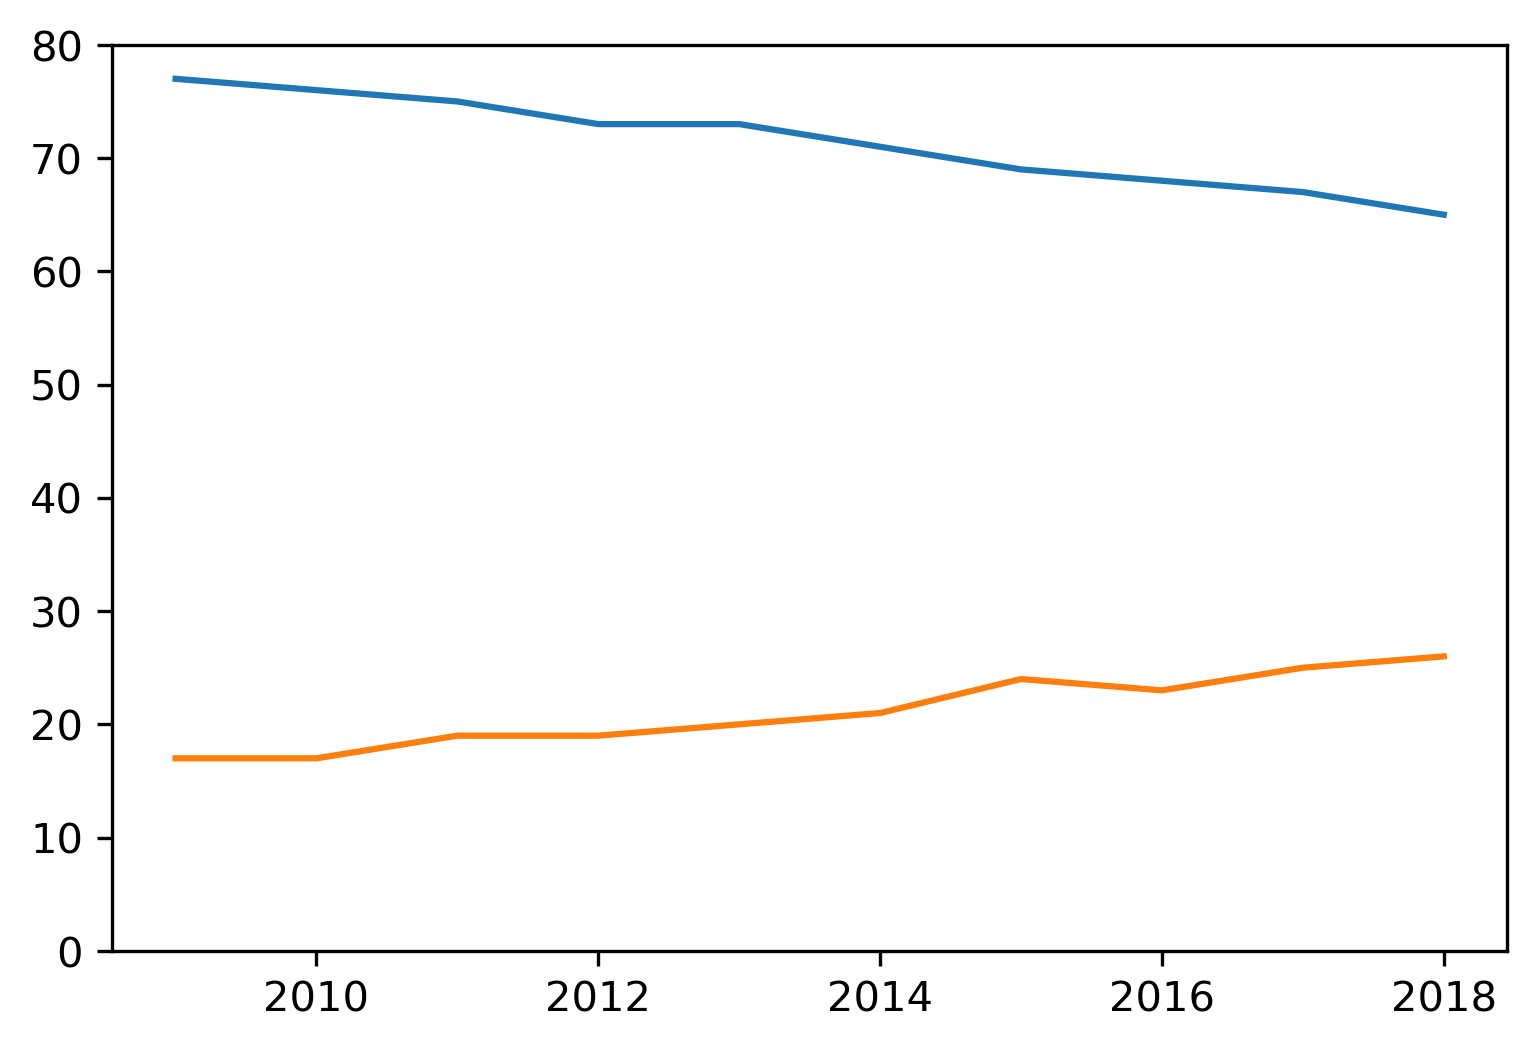
\includegraphics{06_plotting_files/06_plotting_28_0.png}
\caption{png}
\end{figure}

The semi-colon at the end of the line prevents the return value from
\passthrough{\lstinline!plot!}, which is an object representing the
line, from being displayed.

If you plot multiple lines in a single cell, they appear on the same
axes.

\begin{lstlisting}[language=Python]
plt.plot(year, christian)
plt.plot(year, unaffiliated);
\end{lstlisting}

\begin{figure}
\centering
\includegraphics{06_plotting_files/06_plotting_30_0.png}
\caption{png}
\end{figure}

Plotting them on the same axes makes it possible to compare them
directly. However, notice that Pyplot chooses the range for the axes
automatically. In this example the y-axis starts around 15, not zero.

As a result, it provides a misleading picture, making the ratio of the
two lines look bigger than it really is. We can set the limits of the
y-axis using the function \passthrough{\lstinline!plt.ylim!} -- the
arguments are the lower bound and the upper bounds.

\begin{lstlisting}[language=Python]
plt.plot(year, christian)
plt.plot(year, unaffiliated)

plt.ylim(0, 80);
\end{lstlisting}

\begin{figure}
\centering
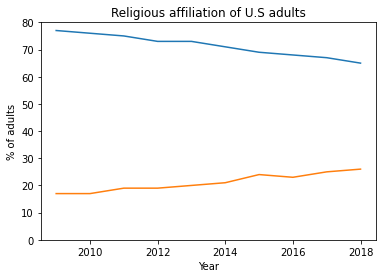
\includegraphics{06_plotting_files/06_plotting_32_0.png}
\caption{png}
\end{figure}

That's better, but this graph is missing some important elements: labels
for the axes, a title, and a legend.

\section{Decorating the Axes}\label{decorating-the-axes}

To label the axes and add a title, we'll use Pyplot functions
\passthrough{\lstinline!xlabel!}, \passthrough{\lstinline!ylabel!}, and
\passthrough{\lstinline!title!}. All of them take strings as arguments.

\begin{lstlisting}[language=Python]
plt.plot(year, christian)
plt.plot(year, unaffiliated)

plt.ylim(0, 80)
plt.xlabel('Year')
plt.ylabel('% of adults')
plt.title('Religious affiliation of U.S adults');
\end{lstlisting}

\begin{figure}
\centering
\includegraphics{06_plotting_files/06_plotting_35_0.png}
\caption{png}
\end{figure}

To add a legend, first we add a label to each line, using the keyword
argument \passthrough{\lstinline!label!}. Then we call
\passthrough{\lstinline!plt.legend!} to create the legend.

\begin{lstlisting}[language=Python]
plt.plot(year, christian, label='Christian')
plt.plot(year, unaffiliated, label='Unaffiliated')

plt.ylim(0, 80)
plt.xlabel('Year')
plt.ylabel('% of adults')
plt.title('Religious affiliation of U.S adults')
plt.legend();
\end{lstlisting}

\begin{figure}
\centering
\includegraphics{06_plotting_files/06_plotting_37_0.png}
\caption{png}
\end{figure}

The legend shows the labels we provided when we created the lines.

\textbf{Exercise:} The original figure plots lines between the data
points, but it also plots markers showing the location of each data
point. It is good practice to include these markers, especially if data
are not available for every year.

Modify the previous example to include a keyword argument
\passthrough{\lstinline!marker!} with the string value
\passthrough{\lstinline!'.'!}, which indicates that you want to plot
small circles as markers.

\textbf{Exercise:} In the original figure, the line labeled
\passthrough{\lstinline!'Christian'!} is red and the line labeled
\passthrough{\lstinline!'Unaffiliated'!} is gray.

Find the online documentation of \passthrough{\lstinline!plt.plot!}, or
ask a virtual assistant like ChatGPT, and figure out how to use keyword
arguments to specify colors. Choose colors to (roughly) match the
original figure.

The \passthrough{\lstinline!legend!} function takes a keyword argument
that specifies the location of the legend. Read the documentation of
this function and move the legend to the center left of the figure.

\section{Plotting Sandwich Prices}\label{plotting-sandwich-prices}

In Chapter 3 we used data from an article in \emph{The Economist}
comparing sandwich prices in Boston and London: ``Why Americans pay more
for lunch than Britons do''.

The article includes this graph showing prices of several sandwiches in
the two cities:

As an exercise, let's see if we can replicate this figure. Here's the
data from the article again.

\begin{lstlisting}[language=Python]
name_list = [
    'Lobster roll',
    'Chicken caesar',
    'Bang bang chicken',
    'Ham and cheese',
    'Tuna and cucumber',
    'Egg'
]
\end{lstlisting}

\begin{lstlisting}[language=Python]
boston_price_list = [9.99, 7.99, 7.49, 7, 6.29, 4.99]
london_price_list = [7.5, 5, 4.4, 5, 3.75, 2.25]
\end{lstlisting}

In the previous section we plotted percentages on the y-axis versus time
on the x-axis. Now we want to plot the sandwich names on the y-axis and
the prices on the x-axis. Here's how:

\begin{lstlisting}[language=Python]
plt.plot(boston_price_list, name_list)
plt.xlabel('Price in USD');
\end{lstlisting}

\begin{figure}
\centering
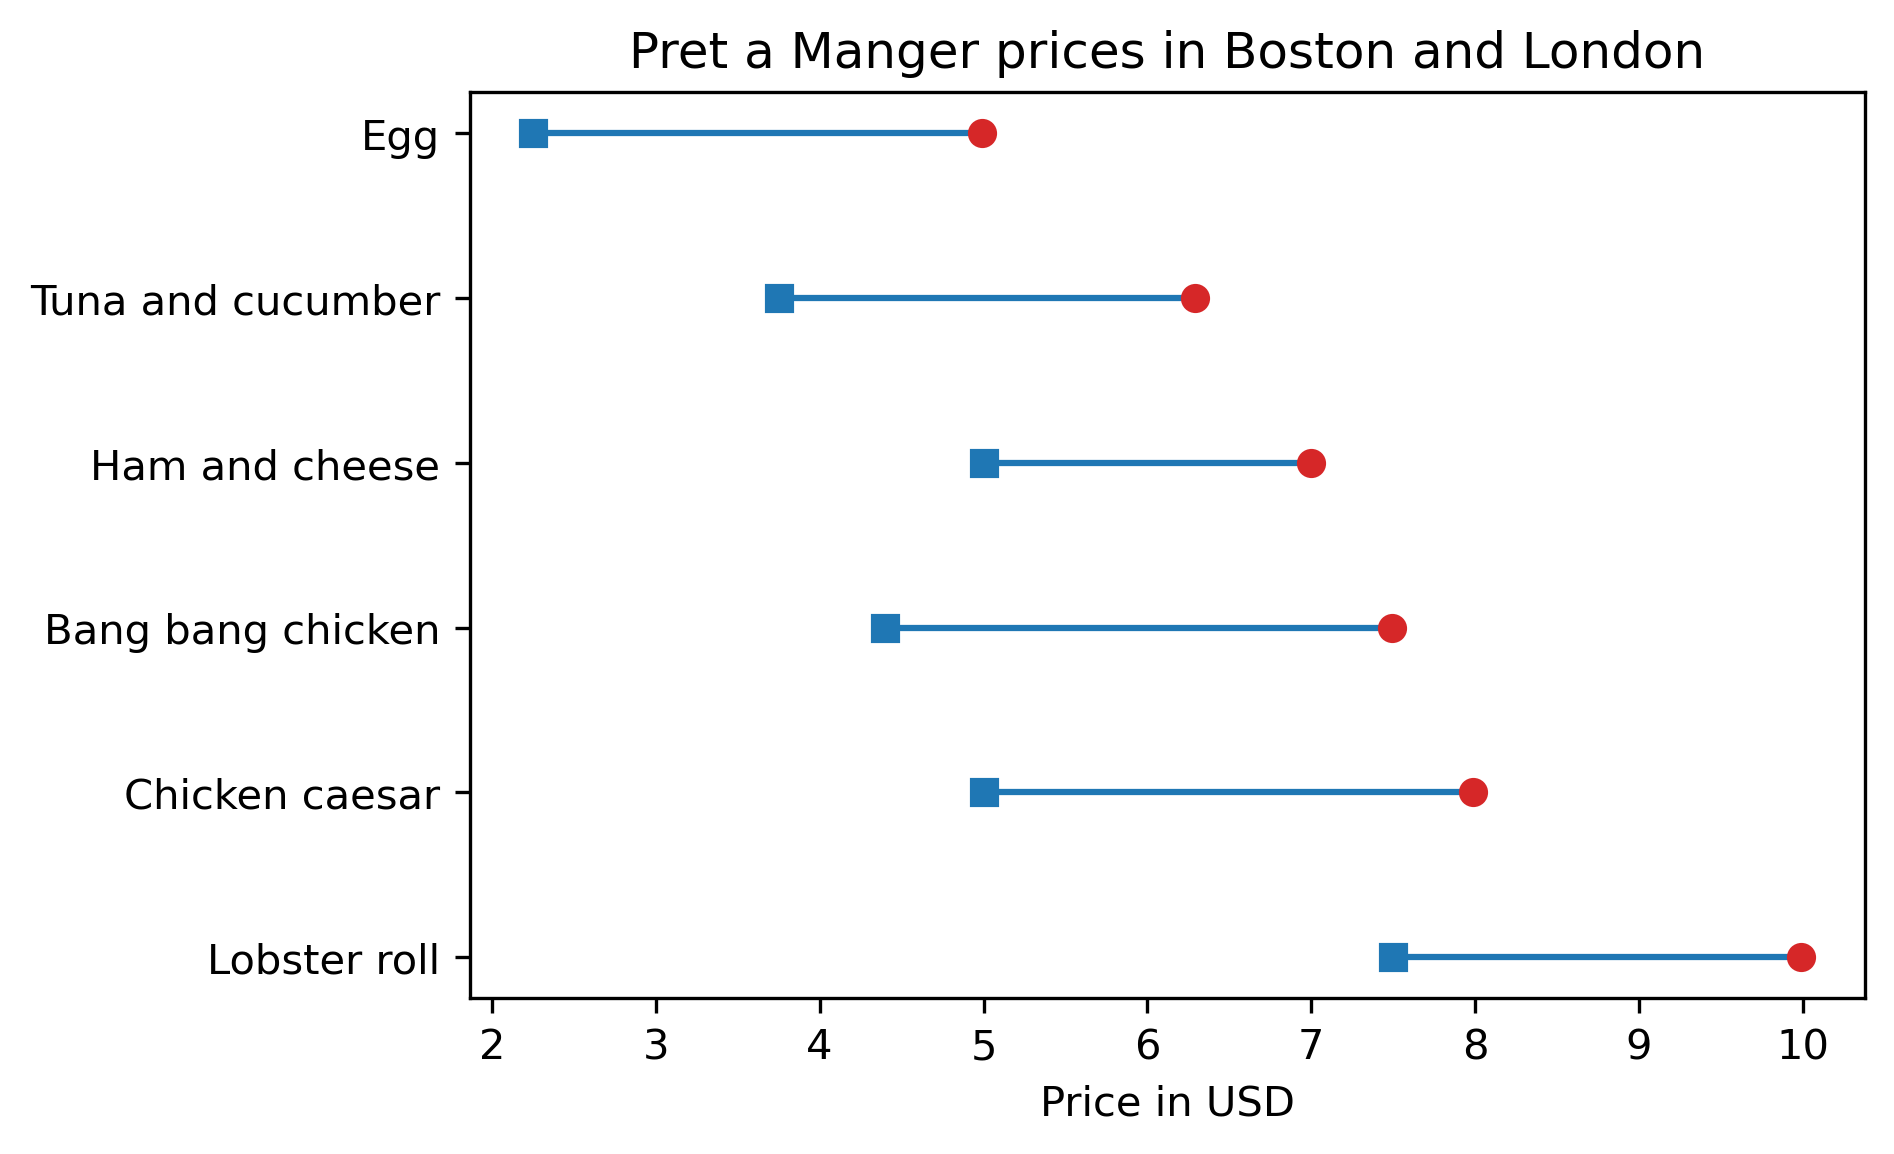
\includegraphics{06_plotting_files/06_plotting_47_0.png}
\caption{png}
\end{figure}

By default Pyplot connects the points with lines, but in this example
the lines don't make sense because the sandwich names are discrete --
that is, there are no intermediate points between an egg sandwich and a
tuna sandwich. We can remove the lines and add markers with the keywords
\passthrough{\lstinline!linestyle!} and
\passthrough{\lstinline!marker!}.

\begin{lstlisting}[language=Python]
plt.plot(boston_price_list, name_list, linestyle='', marker='o')
plt.xlabel('Price in USD');
\end{lstlisting}

\begin{figure}
\centering
\includegraphics{06_plotting_files/06_plotting_49_0.png}
\caption{png}
\end{figure}

Or we can do the same thing more concisely by providing a \textbf{format
string} as a positional argument. In the following examples,
\passthrough{\lstinline!'o'!} indicates a circle marker and
\passthrough{\lstinline!'s'!} indicates a square. You can read the
documentation of \passthrough{\lstinline!plt.plot!} to learn more about
format strings.

\begin{lstlisting}[language=Python]
plt.plot(boston_price_list, name_list, 'o')
plt.plot(london_price_list, name_list, 's')

plt.xlabel('Price in USD')
plt.title('Pret a Manger prices in Boston and London');
\end{lstlisting}

\begin{figure}
\centering
\includegraphics{06_plotting_files/06_plotting_51_0.png}
\caption{png}
\end{figure}

Now, to approximate the colors in the original figure, we can use the
strings \passthrough{\lstinline!'C3'!} and
\passthrough{\lstinline!'C0'!}, which specify colors from the default
color sequence.

\begin{lstlisting}[language=Python]
plt.plot(boston_price_list, name_list, 'o', color='C3')
plt.plot(london_price_list, name_list, 's', color='C0')

plt.xlabel('Price in USD')
plt.title('Pret a Manger prices in Boston and London');
\end{lstlisting}

\begin{figure}
\centering
\includegraphics{06_plotting_files/06_plotting_53_0.png}
\caption{png}
\end{figure}

To connect the dots with lines, we'll use
\passthrough{\lstinline!plt.hlines!}, which draws horizontal lines. It
takes three arguments: a sequence of values on the y-axis, which are the
sandwich names in this example, and two sequences of values on the
x-axis, which are the London prices and Boston prices.

\begin{lstlisting}[language=Python]
plt.hlines(name_list, london_price_list, boston_price_list, color='gray')

plt.plot(boston_price_list, name_list, 'o', color='C3')
plt.plot(london_price_list, name_list, 's', color='C0')

plt.xlabel('Price in USD')
plt.title('Pret a Manger prices in Boston and London');
\end{lstlisting}

\begin{figure}
\centering
\includegraphics{06_plotting_files/06_plotting_55_0.png}
\caption{png}
\end{figure}

\textbf{Exercise:} To finish off this example, add a legend that
identifies the London and Boston prices. Remember that you have to add a
\passthrough{\lstinline!label!} keyword each time you call
\passthrough{\lstinline!plt.plot!}, and then call
\passthrough{\lstinline!plt.legend!}.

Notice that the sandwiches in our figure are in the opposite order of
the sandwiches in the original figure. There is a Pyplot function that
inverts the y-axis; see if you can find it and use it to reverse the
order of the sandwich list.

\section{Zipf's Law}\label{zipfs-law}

In almost any book, in almost any language, if you count the number of
unique words and the number of times each word appears, you will find a
remarkable pattern: the most common word appears twice as often as the
second most common -- at least approximately -- three times as often as
the third most common, and so on.

In general, if we sort the words in descending order of frequency, there
is an inverse relationship between the rank of the words -- first,
second, third, etc. -- and the number of times they appear. This
observation was most famously made by George Kingsley Zipf, so it is
called Zipf's law.

To see if this law holds for the words in \emph{War and Peace}, we'll
make a Zipf plot, which shows:

\begin{itemize}
\item
  The frequency of each word on the y-axis, and
\item
  The rank of each word on the x-axis, starting from 1.
\end{itemize}

In the previous chapter, we looped through the book and made a string
that contains all punctuation characters. Here are the results, which we
will need again.

\begin{lstlisting}[language=Python]
all_punctuation = ',.-:[#]*/“’—‘!?”;()%@'
\end{lstlisting}

The following program reads through the book and makes a dictionary that
maps from each word to the number of times it appears.

\begin{lstlisting}[language=Python]
fp = open('2600-0.txt')
for line in fp:
    if line.startswith('***'):
        break

unique_words = {}
for line in fp:
    if line.startswith('***'):
        break
        
    for word in line.split():
        word = word.lower()
        word = word.strip(all_punctuation)
        if word in unique_words:
            unique_words[word] += 1
        else:
            unique_words[word] = 1
\end{lstlisting}

In \passthrough{\lstinline!unique\_words!}, the keys are words and the
values are their frequencies. We can use the
\passthrough{\lstinline!values!} function to get the values from the
dictionary. The result has the type
\passthrough{\lstinline!dict\_values!}:

\begin{lstlisting}[language=Python]
freqs = unique_words.values()
type(freqs)
\end{lstlisting}

\begin{lstlisting}
dict_values
\end{lstlisting}

Before we plot them, we have to sort them, but the
\passthrough{\lstinline!sort!} function doesn't work with
\passthrough{\lstinline!dict\_values!}.

\begin{lstlisting}[language=Python]
%%expect AttributeError

freqs.sort()
\end{lstlisting}

\begin{lstlisting}
AttributeError: 'dict_values' object has no attribute 'sort'
\end{lstlisting}

We can use \passthrough{\lstinline!list!} to make a list of frequencies:

\begin{lstlisting}[language=Python]
freq_list = list(unique_words.values())
type(freq_list)
\end{lstlisting}

\begin{lstlisting}
list
\end{lstlisting}

And now we can use \passthrough{\lstinline!sort!}. By default it sorts
in ascending order, but we can pass a keyword argument to reverse the
order.

\begin{lstlisting}[language=Python]
freq_list.sort(reverse=True)
\end{lstlisting}

Now, for the ranks, we need a sequence that counts from 1 to
\passthrough{\lstinline!n!}, where \passthrough{\lstinline!n!} is the
number of elements in \passthrough{\lstinline!freq\_list!}. We can use
the \passthrough{\lstinline!range!} function, which returns a value with
type \passthrough{\lstinline!range!}. As a small example, here's the
range from 1 to 5.

\begin{lstlisting}[language=Python]
range(1, 5)
\end{lstlisting}

\begin{lstlisting}
range(1, 5)
\end{lstlisting}

However, there's a catch. If we use the range to make a list, we see
that ``the range from 1 to 5'' includes 1, but it doesn't include 5.

\begin{lstlisting}[language=Python]
list(range(1, 5))
\end{lstlisting}

\begin{lstlisting}
[1, 2, 3, 4]
\end{lstlisting}

That might seem strange, but it is often more convenient to use
\passthrough{\lstinline!range!} when it is defined this way, rather than
what might seem like the more natural way. Anyway, we can get what we
want by increasing the second argument by one:

\begin{lstlisting}[language=Python]
list(range(1, 6))
\end{lstlisting}

\begin{lstlisting}
[1, 2, 3, 4, 5]
\end{lstlisting}

So, finally, we can make a range that represents the ranks from
\passthrough{\lstinline!1!} to \passthrough{\lstinline!n!}:

\begin{lstlisting}[language=Python]
n = len(freq_list)
ranks = range(1, n+1)
ranks
\end{lstlisting}

\begin{lstlisting}
range(1, 20485)
\end{lstlisting}

And now we can plot the frequencies versus the ranks:

\begin{lstlisting}[language=Python]
plt.plot(ranks, freq_list)

plt.xlabel('Rank')
plt.ylabel('Frequency')
plt.title("War and Peace and Zipf's law");
\end{lstlisting}

\begin{figure}
\centering
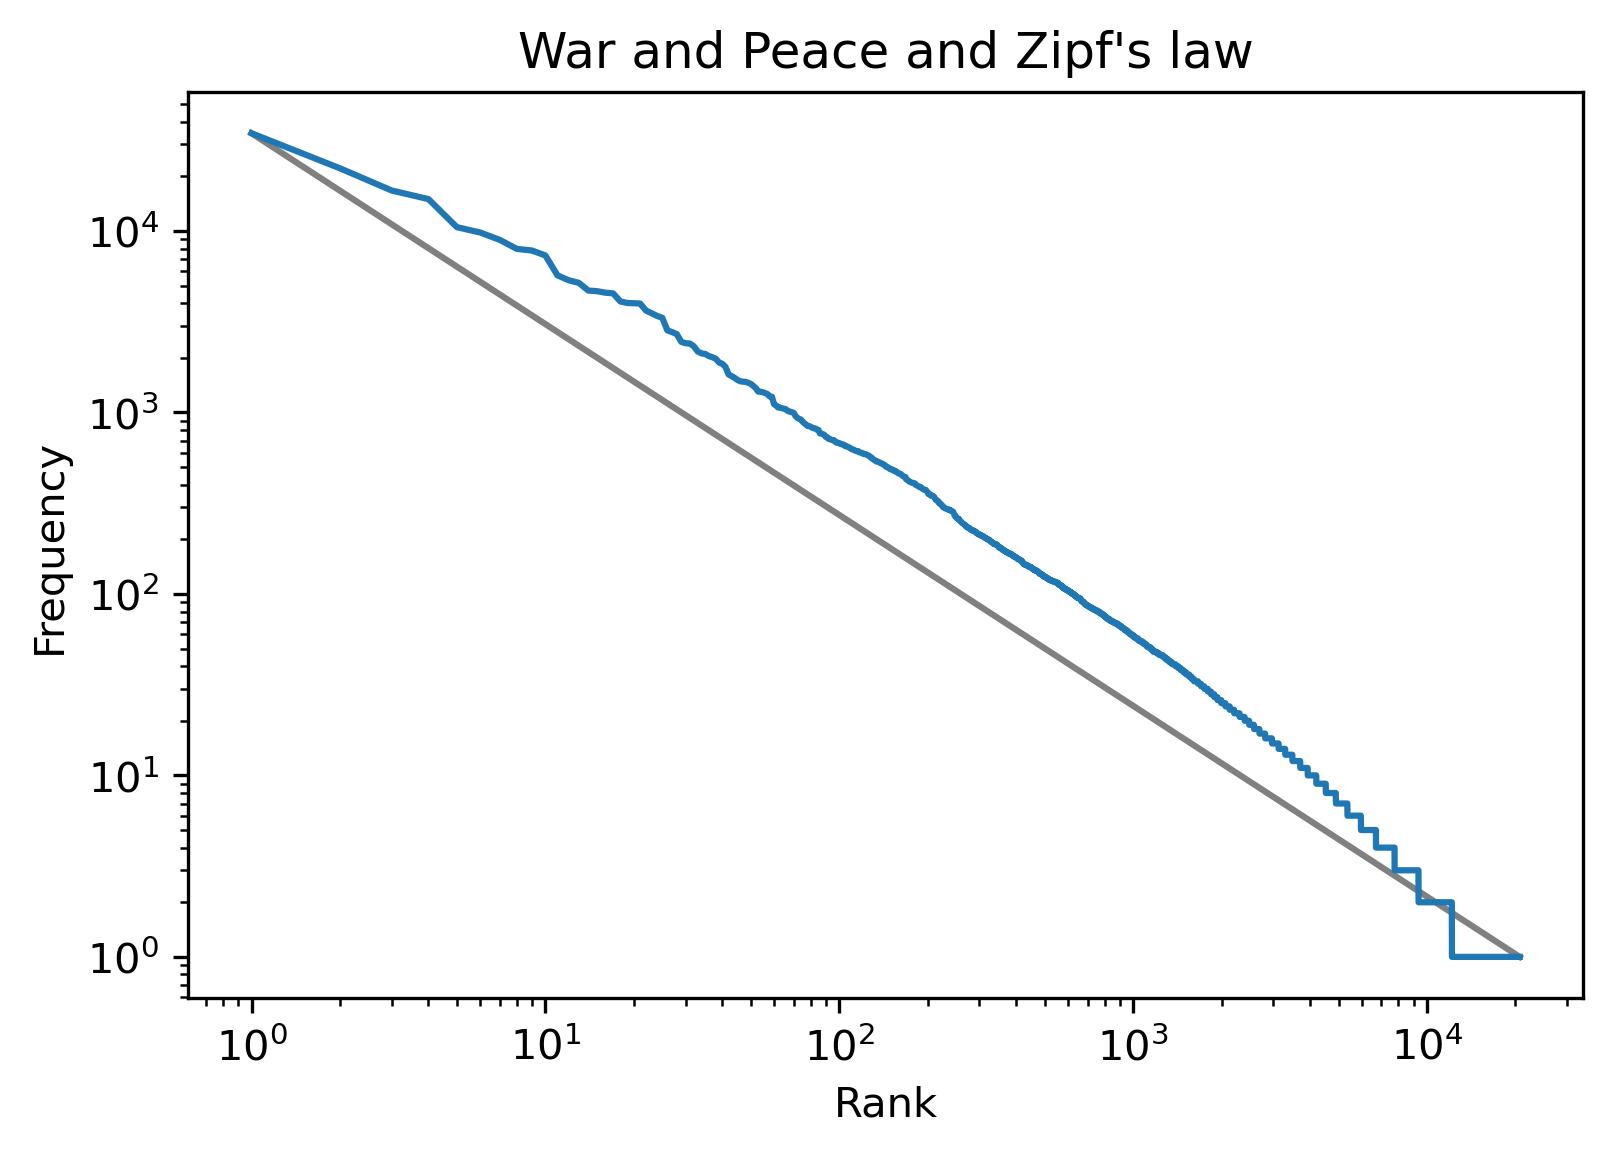
\includegraphics{06_plotting_files/06_plotting_83_0.png}
\caption{png}
\end{figure}

According to Zipf's law, these frequencies should be inversely
proportional to the ranks. If that's true, we can write:

\(f = k / r\)

where \(r\) is the rank of a word, \(f\) is its frequency, and \(k\) is
an unknown constant of proportionality. If we take the logarithm of both
sides, we get

\(\log f = \log k - \log r\)

This equation implies that if we plot \(f\) versus \(r\) on a log-log
scale, we expect to see a straight line with intercept at \(\log k\) and
slope \(-1\).

\section{Logarithmic Scales}\label{logarithmic-scales}

We can use \passthrough{\lstinline!plt.xscale!} to plot the x-axis on a
log scale.

\begin{lstlisting}[language=Python]
plt.plot(ranks, freq_list)

plt.xlabel('Rank')
plt.ylabel('Frequency')
plt.title("War and Peace and Zipf's law")
plt.xscale('log')
\end{lstlisting}

\begin{figure}
\centering
\includegraphics{06_plotting_files/06_plotting_86_0.png}
\caption{png}
\end{figure}

And \passthrough{\lstinline!plt.yscale!} to plot the y-axis on a log
scale.

\begin{lstlisting}[language=Python]
plt.plot(ranks, freq_list)

plt.xlabel('Rank')
plt.ylabel('Frequency')
plt.title("War and Peace and Zipf's law")
plt.xscale('log')
plt.yscale('log')
\end{lstlisting}

\begin{figure}
\centering
\includegraphics{06_plotting_files/06_plotting_88_0.png}
\caption{png}
\end{figure}

The result is not quite a straight line, but it is close. We can get a
sense of the slope by connecting the end points with a line. First,
we'll select the first and last elements from
\passthrough{\lstinline!xs!}.

\begin{lstlisting}[language=Python]
xs = ranks[0], ranks[-1]
xs
\end{lstlisting}

\begin{lstlisting}
(1, 20484)
\end{lstlisting}

And the first and last elements from \passthrough{\lstinline!ys!}.

\begin{lstlisting}[language=Python]
ys = freq_list[0], freq_list[-1]
ys
\end{lstlisting}

\begin{lstlisting}
(34389, 1)
\end{lstlisting}

And plot a line between them.

\begin{lstlisting}[language=Python]
plt.plot(xs, ys, color='gray')
plt.plot(ranks, freq_list)

plt.xlabel('Rank')
plt.ylabel('Frequency')
plt.title("War and Peace and Zipf's law")
plt.xscale('log')
plt.yscale('log')
\end{lstlisting}

\begin{figure}
\centering
\includegraphics{06_plotting_files/06_plotting_94_0.png}
\caption{png}
\end{figure}

The slope of this line is the ``rise over run'', that is, the difference
on the y-axis divided by the difference on the x-axis. We can compute
the rise using \passthrough{\lstinline!np.log10!} to compute the log
base 10 of the first and last values:

\begin{lstlisting}[language=Python]
np.log10(ys)
\end{lstlisting}

\begin{lstlisting}
array([4.53641955, 0.        ])
\end{lstlisting}

Then we can use \passthrough{\lstinline!np.diff!} to compute the
difference between the elements:

\begin{lstlisting}[language=Python]
rise = np.diff(np.log10(ys))
rise
\end{lstlisting}

\begin{lstlisting}
array([-4.53641955])
\end{lstlisting}

\textbf{Exercise:} Use \passthrough{\lstinline!log10!} and
\passthrough{\lstinline!diff!} to compute the run, that is, the
difference on the x-axis. Then divide the rise by the run to get the
slope of the grey line. Is it close to \(-1\), as Zipf's law predicts?

\section{Summary}\label{summary}

This chapter introduces Pyplot, which is part of the Matplotlib library.
We used to replicate two figures and make a Zipf plot. These examples
demonstrate the most common elements of data visualization, including
lines and markers, values and labels on the axes, a legend and a title.
The Zipf plot also shows the power of plotting data on logarithmic
scales.

\backmatter
\end{document}


\hypertarget{dataframes-and-series}{%
\chapter{DataFrames and Series}\label{dataframes-and-series}}

\href{https://colab.research.google.com/github/AllenDowney/ElementsOfDataScience/blob/v1/07_dataframes.ipynb}{Click
here to run this notebook on Colab}.

\begin{lstlisting}[language=Python,style=source]
from os.path import basename, exists

def download(url):
    filename = basename(url)
    if not exists(filename):
        from urllib.request import urlretrieve

        local, _ = urlretrieve(url, filename)
        print("Downloaded " + str(local))
    return filename

download('https://raw.githubusercontent.com/AllenDowney/ElementsOfDataScience/v1/utils.py')

import utils
\end{lstlisting}

This chapter introduces Pandas, a Python library that provides functions
for reading and writing data files, exploring and analyzing data, and
generating visualizations. And it provides two new types for working
with data, \passthrough{\lstinline!DataFrame!} and
\passthrough{\lstinline!Series!}.

We will use these tools to answer a data question -- what is the average
birth weight of babies in the United States? This example will
demonstrate important steps in almost any data science project:

\begin{enumerate}
\def\labelenumi{\arabic{enumi}.}
\item
  Identifying data that can answer a question.
\item
  Obtaining the data and loading it in Python.
\item
  Checking the data and dealing with errors.
\item
  Selecting relevant subsets from the data.
\item
  Using histograms to visualize a distribution of values.
\item
  Using summary statistics to describe the data in a way that best
  answers the question.
\item
  Considering possible sources of error and limitations in our
  conclusions.
\end{enumerate}

Let's start by getting the data.

\hypertarget{reading-the-data}{%
\section{Reading the Data}\label{reading-the-data}}

To estimate average birth weight, we'll use data from the National
Survey of Family Growth (NSFG), which is available from the National
Center for Health Statistics. To download the data, you have to agree to
the Data User's Agreement. URLs for the data and the agreement are in
the notebook for this chapter.

The NSFG data is available from \url{https://www.cdc.gov/nchs/nsfg}.

The Data User's Agreement is at
\url{https://www.cdc.gov/nchs/data_access/ftp_dua.htm}.

You should read the terms carefully, but let me draw your attention to
what I think is the most important one:

\begin{quote}
Make no attempt to learn the identity of any person or establishment
included in these data.
\end{quote}

NSFG respondents answer questions of the most personal nature with the
expectation that their identities will not be revealed. As ethical data
scientists, we should respect their privacy and adhere to the terms of
use.

Respondents to the NSFG provide general information about themselves,
which is stored in the respondent file, and information about each time
they have been pregnant, which is stored in the pregnancy file.

We will work with the pregnancy file, which contains one row for each
pregnancy and one column for each question on the NSFG questionnaire.

The data is stored in a fixed-width format, which means that every row
is the same length and each column spans a fixed range of characters.
For example, the first six characters in each row represent a a unique
identifier for each respondent; the next two characters indicate whether
a pregnancy is the respondent's first, second, etc.

To read this data, we need a \textbf{data dictionary}, which specifies
the names of the columns and the index where each one begins and ends.
The data and the data dictionary are available in separate files.
Instructions for downloading them are in the notebook for this chapter.

\begin{lstlisting}[language=Python,style=source]
dict_file = '2015_2017_FemPregSetup.dct'
data_file = '2015_2017_FemPregData.dat'
\end{lstlisting}

Once you have agreed to the terms, you can use the following cells to
download the data.

\begin{lstlisting}[language=Python,style=source]
download('https://ftp.cdc.gov/pub/health_statistics/nchs/datasets/NSFG/stata/' + dict_file)
\end{lstlisting}

\begin{lstlisting}[style=output]
'2015_2017_FemPregSetup.dct'
\end{lstlisting}

\begin{lstlisting}[language=Python,style=source]
download('https://ftp.cdc.gov/pub/health_statistics/nchs/datasets/NSFG/' + data_file)
\end{lstlisting}

\begin{lstlisting}[style=output]
'2015_2017_FemPregData.dat'
\end{lstlisting}

Pandas can read data in most common formats, including CSV, Excel, and
fixed-width format, but it cannot read the data dictionary, which is in
Stata format. For that, we'll use a Python library called
\passthrough{\lstinline!statadict!}.

The following cell installs \passthrough{\lstinline!statadict!} if
necessary.

\begin{lstlisting}[language=Python,style=source]
try:
    from statadict import parse_stata_dict
except ImportError:
    !pip install statadict
\end{lstlisting}

From \passthrough{\lstinline!statadict!}, we'll import
\passthrough{\lstinline!parse\_stata\_dict!}, which reads the data
dictionary.

\begin{lstlisting}[language=Python,style=source]
from statadict import parse_stata_dict

stata_dict = parse_stata_dict(dict_file)
stata_dict
\end{lstlisting}

\begin{lstlisting}[style=output]
<statadict.base.StataDict at 0x7f091e800a50>
\end{lstlisting}

The result is an object that contains

\begin{itemize}
\item
  \passthrough{\lstinline!names!}, which is a list of column names, and
\item
  \passthrough{\lstinline!colspecs!}, which is a list of tuples, where
  each tuple contains the first and last index of a column.
\end{itemize}

These values are exactly the arguments we need to use
\passthrough{\lstinline!read\_fwf!}, which is the Pandas function that
reads a file in fixed-width format.

\begin{lstlisting}[language=Python,style=source]
import pandas as pd

nsfg = pd.read_fwf(data_file, 
                   names=stata_dict.names, 
                   colspecs=stata_dict.colspecs)
type(nsfg)
\end{lstlisting}

\begin{lstlisting}[style=output]
pandas.core.frame.DataFrame
\end{lstlisting}

The result from \passthrough{\lstinline!read\_fwf()!} is a
\passthrough{\lstinline!DataFrame!}, which is the primary type Pandas
uses to store data. \passthrough{\lstinline!DataFrame!} has a method
called \passthrough{\lstinline!head()!} that shows the first 5 rows:

\begin{lstlisting}[language=Python,style=source]
nsfg.head()
\end{lstlisting}

\begin{lstlisting}[style=output]
   CASEID  PREGORDR  HOWPREG_N  HOWPREG_P  MOSCURRP  NOWPRGDK  PREGEND1  \
0   70627         1        NaN        NaN       NaN       NaN       6.0   
1   70627         2        NaN        NaN       NaN       NaN       1.0   
2   70627         3        NaN        NaN       NaN       NaN       6.0   
3   70628         1        NaN        NaN       NaN       NaN       6.0   
4   70628         2        NaN        NaN       NaN       NaN       6.0   

   PREGEND2  HOWENDDK  NBRNALIV  ...  SECU  SEST  CMINTVW  CMLSTYR  CMJAN3YR  \
0       NaN       NaN       1.0  ...     3   322     1394     1382      1357   
1       NaN       NaN       NaN  ...     3   322     1394     1382      1357   
2       NaN       NaN       1.0  ...     3   322     1394     1382      1357   
3       NaN       NaN       1.0  ...     2   366     1409     1397      1369   
4       NaN       NaN       1.0  ...     2   366     1409     1397      1369   

   CMJAN4YR  CMJAN5YR  QUARTER  PHASE  INTVWYEAR  
0      1345      1333       18      1       2016  
1      1345      1333       18      1       2016  
2      1345      1333       18      1       2016  
3      1357      1345       23      1       2017  
4      1357      1345       23      1       2017  

[5 rows x 248 columns]
\end{lstlisting}

\begin{lstlisting}[language=Python,style=source]
# NOTE: For the printed version of the book, 
# I'm using iloc to show
# the first 5 rows and first 9 columns
\end{lstlisting}

\begin{lstlisting}[language=Python,style=source]
nsfg.iloc[:5,:7]
\end{lstlisting}

\begin{lstlisting}[style=output]
   CASEID  PREGORDR  HOWPREG_N  HOWPREG_P  MOSCURRP  NOWPRGDK  PREGEND1
0   70627         1        NaN        NaN       NaN       NaN       6.0
1   70627         2        NaN        NaN       NaN       NaN       1.0
2   70627         3        NaN        NaN       NaN       NaN       6.0
3   70628         1        NaN        NaN       NaN       NaN       6.0
4   70628         2        NaN        NaN       NaN       NaN       6.0
\end{lstlisting}

The first two columns are \passthrough{\lstinline!CASEID!} and
\passthrough{\lstinline!PREGORDR!}, which I mentioned earlier. The first
three rows have the same \passthrough{\lstinline!CASEID!}, which means
this respondent reported three pregnancies. The values of
\passthrough{\lstinline!PREGORDR!} indicate that they are the first,
second, and third pregnancies, in that order. We will learn more about
the other columns as we go along.

In addition to methods like \passthrough{\lstinline!head!}, a
\passthrough{\lstinline!Dataframe!} object has several
\textbf{attributes}, which are variables associated with the object. For
example, \passthrough{\lstinline!nsfg!} has an attribute called
\passthrough{\lstinline!shape!}, which is a tuple containing the number
of rows and columns:

\begin{lstlisting}[language=Python,style=source]
nsfg.shape
\end{lstlisting}

\begin{lstlisting}[style=output]
(9553, 248)
\end{lstlisting}

There are 9553 rows in this dataset, one for each pregnancy, and 248
columns, one for each question. \passthrough{\lstinline!nsfg!} also has
an attribute called \passthrough{\lstinline!columns!}, which contains
the column names:

\begin{lstlisting}[language=Python,style=source]
nsfg.columns
\end{lstlisting}

\begin{lstlisting}[style=output]
Index(['CASEID', 'PREGORDR', 'HOWPREG_N', 'HOWPREG_P', 'MOSCURRP', 'NOWPRGDK',
       'PREGEND1', 'PREGEND2', 'HOWENDDK', 'NBRNALIV',
       ...
       'SECU', 'SEST', 'CMINTVW', 'CMLSTYR', 'CMJAN3YR', 'CMJAN4YR',
       'CMJAN5YR', 'QUARTER', 'PHASE', 'INTVWYEAR'],
      dtype='object', length=248)
\end{lstlisting}

The column names are stored in an \passthrough{\lstinline!Index!}, which
is another Pandas type, similar to a list.

\begin{lstlisting}[language=Python,style=source]
type(nsfg.columns)
\end{lstlisting}

\begin{lstlisting}[style=output]
pandas.core.indexes.base.Index
\end{lstlisting}

Based on the names, you might be able to guess what some of the columns
are, but in general you have to read the documentation. When you work
with datasets like the NSFG, it is important to read the documentation
carefully. If you interpret a column incorrectly, you can generate
nonsense results and never realize it.

So, before we start looking at data, let's get familiar with the NSFG
codebook, which describes every column. You can download the codebook
for this dataset from
\url{https://github.com/AllenDowney/ElementsOfDataScience/raw/master/data/2015-2017_NSFG_FemPregFile_Codebook-508.pdf}.

If you search that document for ``weigh at birth'' you should find these
columns related to birth weight.

\begin{itemize}
\item
  \passthrough{\lstinline!BIRTHWGT\_LB1!}: Birthweight in Pounds - 1st
  baby from this pregnancy
\item
  \passthrough{\lstinline!BIRTHWGT\_OZ1!}: Birthweight in Ounces - 1st
  baby from this pregnancy
\end{itemize}

There are similar columns for a 2nd or 3rd baby, in the case of twins or
triplets. For now we will focus on the first baby from each pregnancy,
and we will come back to the issue of multiple births.

\hypertarget{series}{%
\section{Series}\label{series}}

In many ways a \passthrough{\lstinline!DataFrame!} is like a Python
dictionary, where the column names are the keys and the columns are the
values. You can select a column from a
\passthrough{\lstinline!DataFrame!} using the bracket operator, with a
string as the key.

\begin{lstlisting}[language=Python,style=source]
pounds = nsfg['BIRTHWGT_LB1']
type(pounds)
\end{lstlisting}

\begin{lstlisting}[style=output]
pandas.core.series.Series
\end{lstlisting}

The result is a \passthrough{\lstinline!Series!}, which is a Pandas type
that represents a single column of data. In this case the
\passthrough{\lstinline!Series!} contains the birth weight, in pounds,
for each live birth.

\passthrough{\lstinline!head!} shows the first five values in the
\passthrough{\lstinline!Series!}, the name of the
\passthrough{\lstinline!Series!}, and the data type:

\begin{lstlisting}[language=Python,style=source]
pounds.head()
\end{lstlisting}

\begin{lstlisting}[style=output]
0    7.0
1    NaN
2    9.0
3    6.0
4    7.0
Name: BIRTHWGT_LB1, dtype: float64
\end{lstlisting}

One of the values is \passthrough{\lstinline!NaN!}, which stands for
``Not a Number''. \passthrough{\lstinline!NaN!} is a special value used
to indicate invalid or missing data. In this example, the pregnancy did
not end in live birth, so birth weight is inapplicable.

\textbf{Exercise:} The column \passthrough{\lstinline!BIRTHWGT\_OZ1!}
contains the ounces part of birth weight.

Select the column \passthrough{\lstinline!'BIRTHWGT\_OZ1'!} from
\passthrough{\lstinline!nsfg!} and assign it to a new variable called
\passthrough{\lstinline!ounces!}. Then display the first 5 elements of
\passthrough{\lstinline!ounces!}.

\textbf{Exercise:} The Pandas types we have seen so far are
\passthrough{\lstinline!DataFrame!}, \passthrough{\lstinline!Index!},
and \passthrough{\lstinline!Series!}. You can find the documentation of
these types at:

\begin{itemize}
\item
  \passthrough{\lstinline!DataFrame!}:
  \url{https://pandas.pydata.org/pandas-docs/stable/reference/api/pandas.DataFrame.html}
\item
  \passthrough{\lstinline!Index!}:
  \url{https://pandas.pydata.org/pandas-docs/stable/reference/api/pandas.Index.html}
\item
  \passthrough{\lstinline!Series!}:
  \url{https://pandas.pydata.org/pandas-docs/stable/reference/api/pandas.Series.html}
\end{itemize}

This documentation can be overwhelming -- I don't recommend trying to
read it all now. But you might want to skim it so you know where to look
later.

\hypertarget{validation}{%
\section{Validation}\label{validation}}

At this point we have identified the columns we need to answer the
question and assigned them to variables named
\passthrough{\lstinline!pounds!} and \passthrough{\lstinline!ounces!}.

\begin{lstlisting}[language=Python,style=source]
pounds = nsfg['BIRTHWGT_LB1']
ounces = nsfg['BIRTHWGT_OZ1']
\end{lstlisting}

Before we do anything with this data, we have to validate it. One part
of validation is confirming that we are interpreting the data correctly.
We can use the \passthrough{\lstinline!value\_counts!} method to see
what values appear in \passthrough{\lstinline!pounds!} and how many
times each value appears.

\begin{lstlisting}[language=Python,style=source]
pounds.value_counts()
\end{lstlisting}

\begin{lstlisting}[style=output]
BIRTHWGT_LB1
7.0     2268
6.0     1644
8.0     1287
5.0      570
9.0      396
4.0      179
99.0      89
10.0      82
3.0       76
2.0       46
1.0       28
11.0      17
0.0        2
12.0       2
98.0       2
13.0       1
14.0       1
Name: count, dtype: int64
\end{lstlisting}

The values are in the left column and the counts are in the right
column. By default, the results are sorted with the highest count first,
but we can use \passthrough{\lstinline!sort\_index!} to sort them by
value instead, with the lightest babies first and heaviest babies last.

\begin{lstlisting}[language=Python,style=source]
pounds.value_counts().sort_index()
\end{lstlisting}

\begin{lstlisting}[style=output]
BIRTHWGT_LB1
0.0        2
1.0       28
2.0       46
3.0       76
4.0      179
5.0      570
6.0     1644
7.0     2268
8.0     1287
9.0      396
10.0      82
11.0      17
12.0       2
13.0       1
14.0       1
98.0       2
99.0      89
Name: count, dtype: int64
\end{lstlisting}

As we'd expect, the most frequent values are
\passthrough{\lstinline!6!}-\passthrough{\lstinline!8!} pounds, but
there are some very light babies, a few very heavy babies, and two
special values, \passthrough{\lstinline!98!}, and
\passthrough{\lstinline!99!}. According to the codebook, these values
indicate that the respondent declined to answer the question
(\passthrough{\lstinline!98!}) or did not know
(\passthrough{\lstinline!99!}).

We can validate the results by comparing them to the codebook, which
lists the values and their frequencies.

\begin{longtable}[]{@{}lll@{}}
\midrule()
value & label & Total \\
\midrule()
\endhead
. & INAPPLICABLE & 2863 \\
0-5 & UNDER 6 POUNDS & 901 \\
6 & 6 POUNDS & 1644 \\
7 & 7 POUNDS & 2268 \\
8 & 8 POUNDS & 1287 \\
9-95 & 9 POUNDS OR MORE & 499 \\
98 & Refused & 2 \\
99 & Don't know & 89 \\
& Total & 9553 \\
\midrule()
\end{longtable}

The results from \passthrough{\lstinline!value\_counts!} agree with the
codebook, so we have some confidence that we are reading and
interpreting the data correctly.

\textbf{Exercise:} In \passthrough{\lstinline!nsfg!}, the column
\passthrough{\lstinline!'OUTCOME'!} encodes the outcome of each
pregnancy as shown below:

\begin{longtable}[]{@{}ll@{}}
\midrule()
Value & Meaning \\
\midrule()
\endhead
1 & Live birth \\
2 & Induced abortion \\
3 & Stillbirth \\
4 & Miscarriage \\
5 & Ectopic pregnancy \\
6 & Current pregnancy \\
\midrule()
\end{longtable}

Use \passthrough{\lstinline!value\_counts!} to display the values in
this column and how many times each value appears. Are the results
consistent with the codebook?

\hypertarget{summary-statistics}{%
\section{Summary Statistics}\label{summary-statistics}}

Another way to validate the data is with
\passthrough{\lstinline!describe!}, which computes statistics that
summarize the data, like the mean, standard deviation, minimum, and
maximum. Here are the results for \passthrough{\lstinline!pounds!}.

\begin{lstlisting}[language=Python,style=source]
pounds.describe()
\end{lstlisting}

\begin{lstlisting}[style=output]
count    6690.000000
mean        8.008819
std        10.771360
min         0.000000
25%         6.000000
50%         7.000000
75%         8.000000
max        99.000000
Name: BIRTHWGT_LB1, dtype: float64
\end{lstlisting}

\passthrough{\lstinline!count!} is the number of values, not including
\passthrough{\lstinline!NaN!}. In this column, there are 6690 value that
are not \passthrough{\lstinline!NaN!}. \passthrough{\lstinline!mean!}
and \passthrough{\lstinline!std!} are the mean and standard deviation.
\passthrough{\lstinline!min!} and \passthrough{\lstinline!max!} are the
minimum and maximum values, and in between are the 25th, 50th, and 75th
percentiles. The 50th percentile is the median.

The mean is about \passthrough{\lstinline!8.05!}, but that doesn't mean
much because it includes the special values \passthrough{\lstinline!98!}
and \passthrough{\lstinline!99!}. Before we can really compute the mean,
we have to replace those values with \passthrough{\lstinline!NaN!} to
identify them as missing data. The \passthrough{\lstinline!replace()!}
method does what we want:

\begin{lstlisting}[language=Python,style=source]
import numpy as np

pounds_clean = pounds.replace([98, 99], np.nan)
\end{lstlisting}

\passthrough{\lstinline!replace!} takes a list of the values we want to
replace and the value we want to replace them with.
\passthrough{\lstinline!np.nan!} means we are getting the special value
\passthrough{\lstinline!NaN!} from the NumPy library, which is imported
as \passthrough{\lstinline!np!}. The result from
\passthrough{\lstinline!replace()!} is a new
\passthrough{\lstinline!Series!}, which I assign to
\passthrough{\lstinline!pounds\_clean!}. If we run
\passthrough{\lstinline!describe!} again, we see that
\passthrough{\lstinline!count!} is smaller now because it includes only
the valid values.

\begin{lstlisting}[language=Python,style=source]
pounds_clean.describe()
\end{lstlisting}

\begin{lstlisting}[style=output]
count    6599.000000
mean        6.754357
std         1.383268
min         0.000000
25%         6.000000
50%         7.000000
75%         8.000000
max        14.000000
Name: BIRTHWGT_LB1, dtype: float64
\end{lstlisting}

The mean of the new \passthrough{\lstinline!Series!} is about
\passthrough{\lstinline!6.7!} pounds. Remember that the mean of the
original \passthrough{\lstinline!Series!} was more than
\passthrough{\lstinline!8!} pounds. It makes a big difference when you
remove a few \passthrough{\lstinline!99!}-pound babies!

\textbf{Exercise:} Use \passthrough{\lstinline!describe!} to summarize
\passthrough{\lstinline!ounces!}.\\
Then use \passthrough{\lstinline!replace!} to replace the special values
\passthrough{\lstinline!98!} and \passthrough{\lstinline!99!} with
\passthrough{\lstinline!NaN!}, and assign the result to
\passthrough{\lstinline!ounces\_clean!}. Run
\passthrough{\lstinline!describe!} again. How much does this cleaning
affect the results?

\hypertarget{series-arithmetic}{%
\section{Series Arithmetic}\label{series-arithmetic}}

Now we want to combine \passthrough{\lstinline!pounds!} and
\passthrough{\lstinline!ounces!} into a single
\passthrough{\lstinline!Series!} that contains total birth weight.
Arithmetic operators work with \passthrough{\lstinline!Series!} objects
-- for example, to convert \passthrough{\lstinline!pounds!} to ounces,
we could write

\passthrough{\lstinline!pounds * 16!}

Then we could add in \passthrough{\lstinline!ounces!} like this

\passthrough{\lstinline!pounds * 16 + ounces!}

\textbf{Exercise:} Use \passthrough{\lstinline!pounds\_clean!} and
\passthrough{\lstinline!ounces\_clean!} to compute the total birth
weight expressed in kilograms (there are roughly 2.2 pounds per
kilogram). What is the mean birth weight in kilograms?

\hypertarget{histograms}{%
\section{Histograms}\label{histograms}}

Let's get back to the original question: what is the average birth
weight for babies in the U.S.?\\
As an answer we \emph{could} take the results from the previous section
and compute the mean:

\begin{lstlisting}[language=Python,style=source]
pounds_clean = pounds.replace([98, 99], np.nan)
ounces_clean = ounces.replace([98, 99], np.nan)

birth_weight = pounds_clean + ounces_clean / 16
birth_weight.mean()
\end{lstlisting}

\begin{lstlisting}[style=output]
7.180217889908257
\end{lstlisting}

But it is risky to compute a summary statistic, like the mean, before we
look at the whole distribution of values. A \textbf{distribution} is a
set of possible values and their frequencies. One way to visualize a
distribution is a \textbf{histogram}, which shows values on the
\passthrough{\lstinline!x!} axis and their frequencies on the
\passthrough{\lstinline!y!} axis. \passthrough{\lstinline!Series!}
provides a \passthrough{\lstinline!hist!} method that makes histograms,
and we can use Pyplot to label the axes.

\begin{lstlisting}[language=Python,style=source]
import matplotlib.pyplot as plt

birth_weight.hist(bins=30)
plt.xlabel('Birth weight in pounds')
plt.ylabel('Number of live births')
plt.title('Distribution of U.S. birth weight');
\end{lstlisting}

\begin{center}
\includegraphics[width=4in]{chapters/07_dataframes_files/07_dataframes_62_0.png}
\end{center}

The keyword argument, \passthrough{\lstinline!bins!}, tells
\passthrough{\lstinline!hist!} to divide the range of weights into 30
intervals, called \textbf{bins}, and count how many values fall in each
bin. The \passthrough{\lstinline!x!} axis is birth weight in pounds; the
\passthrough{\lstinline!y!} axis is the number of births in each bin.

The distribution looks like a bell curve, but the tail is longer on the
left than on the right -- that is, there are more light babies than
heavy babies. That makes sense, because the distribution includes some
babies that were born preterm.

\textbf{Exercise:} \passthrough{\lstinline!hist!} takes keyword
arguments that specify the type and appearance of the histogram. Find
the documentation of \passthrough{\lstinline!hist!} and see if you can
figure out how to plot the histogram as an unfilled line against a
background with no grid lines.

\textbf{Exercise:} The NSFG dataset includes a column called
\passthrough{\lstinline!AGECON!} that records a woman's age at
conception for each pregnancy.

\begin{itemize}
\item
  Select this column from the \passthrough{\lstinline!DataFrame!} and
  plot the histogram of the values with 20 bins.
\item
  Label the \passthrough{\lstinline!x!} and \passthrough{\lstinline!y!}
  axes appropriately.
\end{itemize}

\hypertarget{boolean-series}{%
\section{Boolean Series}\label{boolean-series}}

We have seen that the distribution of birth weights is \textbf{skewed}
to the left -- that is, there are more light babies than heavy ones and
they are farther from the mean. That's because preterm babies tend to be
lighter. The most common duration for pregnancy is 39 weeks, which is
``full term''; ``preterm'' is usually defined to be less than 37 weeks.

To see which babies are preterm, we can use the
\passthrough{\lstinline!PRGLNGTH!} column, which records pregnancy
length in weeks.

\begin{lstlisting}[language=Python,style=source]
preterm = (nsfg['PRGLNGTH'] < 37)
preterm.dtype
\end{lstlisting}

\begin{lstlisting}[style=output]
dtype('bool')
\end{lstlisting}

When you compare a \passthrough{\lstinline!Series!} to a value, the
result is a Boolean \passthrough{\lstinline!Series!} -- that is, a
\passthrough{\lstinline!Series!} where each element is a Boolean value,
\passthrough{\lstinline!True!} or \passthrough{\lstinline!False!}. In
this case, it's \passthrough{\lstinline!True!} for each preterm baby and
\passthrough{\lstinline!False!} otherwise. We can use
\passthrough{\lstinline!head!} to see the first 5 elements.

\begin{lstlisting}[language=Python,style=source]
preterm.head()
\end{lstlisting}

\begin{lstlisting}[style=output]
0    False
1     True
2    False
3    False
4    False
Name: PRGLNGTH, dtype: bool
\end{lstlisting}

If you compute the sum of a Boolean \passthrough{\lstinline!Series!}, it
treats \passthrough{\lstinline!True!} as 1 and
\passthrough{\lstinline!False!} as 0, so the sum is the number of
\passthrough{\lstinline!True!} values, which is the number of preterm
babies.

\begin{lstlisting}[language=Python,style=source]
preterm.sum()
\end{lstlisting}

\begin{lstlisting}[style=output]
3675
\end{lstlisting}

If you compute the mean of a Boolean \passthrough{\lstinline!Series!},
you get the \emph{fraction} of \passthrough{\lstinline!True!} values. In
this case, it's about \passthrough{\lstinline!0.38!} -- that is, about
38\% of the pregnancies are less than \passthrough{\lstinline!37!}
weeks.

\begin{lstlisting}[language=Python,style=source]
preterm.mean()
\end{lstlisting}

\begin{lstlisting}[style=output]
0.38469590704490736
\end{lstlisting}

However, this result might be misleading because it includes all
pregnancy outcomes, not just live births. We can create another Boolean
\passthrough{\lstinline!Series!} to indicate which pregnancies ended in
live birth:

\begin{lstlisting}[language=Python,style=source]
live = (nsfg['OUTCOME'] == 1)
live.mean()
\end{lstlisting}

\begin{lstlisting}[style=output]
0.7006176070344394
\end{lstlisting}

Now we can use the operator \passthrough{\lstinline!\&!}, which
represents the logical AND operation, to identify pregnancies where the
outcome is a live birth \emph{and} preterm:

\begin{lstlisting}[language=Python,style=source]
live_preterm = (live & preterm)
live_preterm.mean()
\end{lstlisting}

\begin{lstlisting}[style=output]
0.08929132209777034
\end{lstlisting}

About \(9\%\) of all pregnancies resulted in a preterm live birth.

The other common logical operators that work with
\passthrough{\lstinline!Series!} objects are:

\begin{itemize}
\item
  \passthrough{\lstinline!|!}, which represents the logical OR operation
  -- for example, \passthrough{\lstinline!live | preterm!} is true if
  either \passthrough{\lstinline!live!} is true, or
  \passthrough{\lstinline!preterm!} is true, or both.
\item
  \passthrough{\lstinline!\~!}, which represents the logical NOT
  operation -- for example, \passthrough{\lstinline!\~live!} is true if
  \passthrough{\lstinline!live!} is false or
  \passthrough{\lstinline!NaN!}.
\end{itemize}

The logical operators treat \passthrough{\lstinline!NaN!} the same as
\passthrough{\lstinline!False!}, so you should be careful about using
the NOT operator with a Series that contains
\passthrough{\lstinline!NaN!} values. For example,
\passthrough{\lstinline!\~preterm!} would include not just full term
pregnancies, but also pregnancies with unknown length.

\textbf{Exercise:} Of all pregnancies, what fraction are live births at
full term (\passthrough{\lstinline!37!} weeks or more)? Of all live
births, what fraction are full term?

\hypertarget{filtering-data}{%
\section{Filtering Data}\label{filtering-data}}

We can use a Boolean \passthrough{\lstinline!Series!} as a filter --
that is, we can select only rows that satisfy a condition or meet some
criterion. For example, we can use \passthrough{\lstinline!preterm!} and
the bracket operator to select values from
\passthrough{\lstinline!birth\_weight!}, so
\passthrough{\lstinline!preterm\_weight!} gets birth weights for preterm
babies.

\begin{lstlisting}[language=Python,style=source]
preterm_weight = birth_weight[preterm]
preterm_weight.mean()
\end{lstlisting}

\begin{lstlisting}[style=output]
5.480958781362007
\end{lstlisting}

To select full-term babies, we can create a Boolean
\passthrough{\lstinline!Series!} like this:

\begin{lstlisting}[language=Python,style=source]
fullterm = (nsfg['PRGLNGTH'] >= 37)
\end{lstlisting}

And use it to select birth weights for full term babies:

\begin{lstlisting}[language=Python,style=source]
full_term_weight = birth_weight[fullterm]
full_term_weight.mean()
\end{lstlisting}

\begin{lstlisting}[style=output]
7.429609416096791
\end{lstlisting}

As expected, full term babies are heavier, on average, than preterm
babies. To be more explicit, we could also limit the results to live
births, like this:

\begin{lstlisting}[language=Python,style=source]
full_term_weight = birth_weight[live & fullterm]
full_term_weight.mean()
\end{lstlisting}

\begin{lstlisting}[style=output]
7.429609416096791
\end{lstlisting}

But in this case we get the same result because
\passthrough{\lstinline!birth\_weight!} is only valid for live births.

\textbf{Exercise:} Let's see if there is a difference in weight between
single births and multiple births (twins, triplets, etc.). The column
\passthrough{\lstinline!NBRNALIV!} represents the number of babies born
alive from a single pregnancy.

\begin{lstlisting}[language=Python,style=source]
nbrnaliv = nsfg['NBRNALIV']
nbrnaliv.value_counts()
\end{lstlisting}

\begin{lstlisting}[style=output]
NBRNALIV
1.0    6573
2.0     111
3.0       6
Name: count, dtype: int64
\end{lstlisting}

Use \passthrough{\lstinline!nbrnaliv!} and
\passthrough{\lstinline!live!} to create a Boolean series called
\passthrough{\lstinline!multiple!} that is true for multiple live
births. Of all live births, what fraction are multiple births?

\textbf{Exercise:} Make a Boolean series called
\passthrough{\lstinline!single!} that is true for single live births. Of
all single births, what fraction are preterm? Of all multiple births,
what fraction are preterm?

\textbf{Exercise:} What is the average birth weight for live, single,
full-term births?

\hypertarget{weighted-means}{%
\section{Weighted Means}\label{weighted-means}}

We are almost done, but there's one more problem we have to solve:
oversampling.

The NSFG sample is not exactly representative of the U.S. population. By
design, some groups are more likely to appear in the sample than others
-- that is, they are \textbf{oversampled}. Oversampling helps to ensure
that you have enough people in every group to get reliable statistics,
but it makes data analysis a little more complicated.

Each pregnancy in the dataset has a \textbf{sampling weight} that
indicates how many pregnancies it represents. In
\passthrough{\lstinline!nsfg!}, the sampling weight is stored in a
column named \passthrough{\lstinline!wgt2015\_2017!}. Here's what it
looks like.

\begin{lstlisting}[language=Python,style=source]
sampling_weight = nsfg['WGT2015_2017']
sampling_weight.describe()
\end{lstlisting}

\begin{lstlisting}[style=output]
count      9553.000000
mean      13337.425944
std       16138.878271
min        1924.916000
25%        4575.221221
50%        7292.490835
75%       15724.902673
max      106774.400000
Name: WGT2015_2017, dtype: float64
\end{lstlisting}

The median value (\passthrough{\lstinline!50!}th percentile) in this
column is about \passthrough{\lstinline!7292!}, which means that a
pregnancy with that weight represents \passthrough{\lstinline!7292!}
total pregnancies in the population. But the range of values is wide, so
some rows represent many more pregnancies than others.

To take these weights into account, we can compute a \textbf{weighted
mean}. Here are the steps:

\begin{enumerate}
\def\labelenumi{\arabic{enumi}.}
\item
  Multiply the birth weights for each pregnancy by the sampling weights
  and add up the products.
\item
  Add up the sampling weights.
\item
  Divide the first sum by the second.
\end{enumerate}

To do this correctly, we have to be careful with missing data. To help
with that, we'll use two \passthrough{\lstinline!Series!} methods,
\passthrough{\lstinline!isna!} and \passthrough{\lstinline!notna!}.
\passthrough{\lstinline!isna!} returns a Boolean
\passthrough{\lstinline!Series!} that is \passthrough{\lstinline!True!}
where the corresponding value is \passthrough{\lstinline!NaN!}.

\begin{lstlisting}[language=Python,style=source]
missing = birth_weight.isna()
missing.sum()
\end{lstlisting}

\begin{lstlisting}[style=output]
3013
\end{lstlisting}

In \passthrough{\lstinline!birth\_weight!} there are
\passthrough{\lstinline!3013!} missing values (mostly for pregnancies
that did not end in live birth). \passthrough{\lstinline!notna!} returns
a Boolean \passthrough{\lstinline!Series!} that is
\passthrough{\lstinline!True!} where the corresponding value is
\emph{not} \passthrough{\lstinline!NaN!}.

\begin{lstlisting}[language=Python,style=source]
valid = birth_weight.notna()
valid.sum()
\end{lstlisting}

\begin{lstlisting}[style=output]
6540
\end{lstlisting}

We can combine \passthrough{\lstinline!valid!} with the other Boolean
\passthrough{\lstinline!Series!} we have computed to identify single,
full term, live births with valid birth weights.

\begin{lstlisting}[language=Python,style=source]
single = (nbrnaliv == 1)
selected = valid & live & single & fullterm
selected.sum()
\end{lstlisting}

\begin{lstlisting}[style=output]
5648
\end{lstlisting}

You can finish off this computation as an exercise.

\textbf{Exercise:} Use \passthrough{\lstinline!selected!},
\passthrough{\lstinline!birth\_weight!}, and
\passthrough{\lstinline!sampling\_weight!} to compute the weighted mean
of birth weight for live, single, full term births. You should find that
the weighted mean is a little higher than the unweighted mean we
computed in the previous section. That's because the groups that are
oversampled in the NSFG tend to have lighter babies, on average.

\hypertarget{summary}{%
\section{Summary}\label{summary}}

This chapter poses what seems like a simple question: what is the
average birth weight of babies in the United States?

To answer it, we found an appropriate dataset and downloaded the files.
We used Pandas to read the files and create a
\passthrough{\lstinline!DataFrame!}. Then we validated the data and
dealt with special values and missing data. To explore the data, we used
\passthrough{\lstinline!value\_counts!}, \passthrough{\lstinline!hist!},
\passthrough{\lstinline!describe!}, and other methods. And to select
relevant data, we used Boolean \passthrough{\lstinline!Series!} objects.

Along the way, we had to think more about the question. What do we mean
by ``average'', and which babies should we include? Should we include
all live births or exclude preterm babies or multiple births?

And we had to think about the sampling process. By design, the NSFG
respondents are not representative of the U.S. population, but we can
use sampling weights to correct for this effect.

Even a simple question can be a challenging data science project.

A note on vocabulary: In a dataset like the one we used in this chapter,
we could say that each column represents a ``variable'', and what we
called column names might also be called variable names. I avoided that
use of the term because it might be confusing to say that we select a
``variable'' from a \passthrough{\lstinline!DataFrame!} and assign it to
a Python variable. But you might see this use of the term elsewhere, so
I thought I would mention it.

\emph{Elements of Data Science}

Copyright 2021 \href{https://allendowney.com}{Allen B. Downey}

License:
\href{https://creativecommons.org/licenses/by-nc-sa/4.0/}{Creative
Commons Attribution-NonCommercial-ShareAlike 4.0 International}




\part{Exploratory Data Analysis}

\hypertarget{distributions}{%
\chapter{Distributions}\label{distributions}}

In this chapter we'll see three ways to describe a distribution:

\begin{itemize}
\item
  A probability mass function (PMF), which represents a set of values
  and the number of times each one appears in a dataset.
\item
  A cumulative distribution function (CDF), which contains the same
  information as a PMF in a form that makes it easier to visualize, make
  comparisons, and perform some computations.
\item
  A kernel density estimate (KDE), which is like a smooth, continuous
  version of a histogram.
\end{itemize}

As examples, we'll use data from the General Social Survey (GSS) to look
at distributions of age and income, and to explore the relationship
between income and education. But we'll start with one of the most
important ideas in statistics, the distribution.

\hypertarget{distributions-1}{%
\section{Distributions}\label{distributions-1}}

A distribution is a set of values and their corresponding probabilities.
For example, if you roll a six-sided die, there are six possible
outcomes, the numbers \passthrough{\lstinline!1!} through
\passthrough{\lstinline!6!}, and they all have the same probability,
\passthrough{\lstinline!1/6!}. We can represent this distribution of
outcomes with a table, like this:

\begin{longtable}[]{@{}ll@{}}
\midrule()
Value & Probability \\
\midrule()
\endhead
1 & 1/6 \\
2 & 1/6 \\
3 & 1/6 \\
4 & 1/6 \\
5 & 1/6 \\
6 & 1/6 \\
\midrule()
\end{longtable}

More generally, a distribution can have any number of values, the values
can be any type, and the probabilities do not have to be equal. To
represent distributions in Python, we will use a library called
\passthrough{\lstinline!empiricaldist!}, for ``empirical distribution'',
where ``empirical'' means it is based on data rather than a mathematical
formula.

\passthrough{\lstinline!empiricaldist!} provides an object called
\passthrough{\lstinline!Pmf!}, which stands for ``probability mass
function''. A \passthrough{\lstinline!Pmf!} object contains a set of
possible outcomes and their probabilities. For example, here's a
\passthrough{\lstinline!Pmf!} that represents the outcome of rolling a
six-sided die:

\begin{lstlisting}[language=Python,style=source]
from empiricaldist import Pmf

outcomes = [1,2,3,4,5,6]
die = Pmf(1/6, outcomes)
\end{lstlisting}

The first argument is the probability of each outcome; the second
argument is the list of outcomes. We can display the result like this.

\begin{lstlisting}[language=Python,style=source]
die
\end{lstlisting}

\begin{lstlisting}[style=output]
1    0.166667
2    0.166667
3    0.166667
4    0.166667
5    0.166667
6    0.166667
dtype: float64
\end{lstlisting}

A \passthrough{\lstinline!Pmf!} object is a specialized version of a
Pandas \passthrough{\lstinline!Series!}, so it provides all of the
attributes and methods of a \passthrough{\lstinline!Series!}, plus some
additional methods we'll see soon.

\hypertarget{the-general-social-survey}{%
\section{The General Social Survey}\label{the-general-social-survey}}

Now we'll use \passthrough{\lstinline!Pmf!} objects to represent
distributions of values from a new dataset, the General Social Survey
(GSS). The GSS surveys a representative sample of adult residents of the
U.S. and asks questions about demographics, personal history, and
beliefs about social and political issues. It is widely used by
politicians, policy makers, and researchers.

The GSS dataset contains hundreds of columns; using an online tool call
\href{https://gssdataexplorer.norc.org/}{GSS Explorer} I've selected
just a few and created a subset of the data, called an \textbf{extract}.
I have stored the data in an HDF file, which is more compact than the
original fixed-width file, and faster to read. Instructions for
downloading the files are in the notebook for this chapter.

\begin{lstlisting}[language=Python,style=source]
data_file = 'gss_extract_2022.hdf'
\end{lstlisting}

We'll use \passthrough{\lstinline!pd.read\_hdf!} to read the data file
and extract from it \passthrough{\lstinline!gss!}, which is a
\passthrough{\lstinline!DataFrame!}.

\begin{lstlisting}[language=Python,style=source]
import pandas as pd

gss = pd.read_hdf(data_file, 'gss')
gss.shape
\end{lstlisting}

\begin{lstlisting}[style=output]
(72390, 9)
\end{lstlisting}

The result is a \passthrough{\lstinline!DataFrame!} with one row for
each respondent, and one column for each question in the extract. Here
are the first few rows.

\begin{lstlisting}[language=Python,style=source]
gss.head()
\end{lstlisting}

\begin{lstlisting}[style=output]
   year  id   age  educ  degree  sex  gunlaw  grass  realinc
0  1972   1  23.0  16.0     3.0  2.0     1.0    NaN  18951.0
1  1972   2  70.0  10.0     0.0  1.0     1.0    NaN  24366.0
2  1972   3  48.0  12.0     1.0  2.0     1.0    NaN  24366.0
3  1972   4  27.0  17.0     3.0  2.0     1.0    NaN  30458.0
4  1972   5  61.0  12.0     1.0  2.0     1.0    NaN  50763.0
\end{lstlisting}

I'll explain these columns as we go along, but if you want more
information, you can read the online documentation at
\url{https://gssdataexplorer.norc.org/variables/vfilter}. In the GSS
documentation, you'll see that they use the term ``variable'' for a
column that contains answers to survey questions.

\hypertarget{distribution-of-education}{%
\section{Distribution of Education}\label{distribution-of-education}}

To get started with this dataset, let's look at the distribution of
\passthrough{\lstinline!educ!}, which records the number of years of
education for each respondent. First we'll select a column from the
\passthrough{\lstinline!DataFrame!} and use
\passthrough{\lstinline!value\_counts!} to see what values are in it.

\begin{lstlisting}[language=Python,style=source]
gss['educ'].value_counts().sort_index()
\end{lstlisting}

\begin{lstlisting}[style=output]
educ
0.0       177
1.0        49
2.0       158
3.0       268
4.0       326
5.0       410
6.0       866
7.0       896
8.0      2786
9.0      2172
10.0     3010
11.0     3942
12.0    21401
13.0     5905
14.0     8208
15.0     3307
16.0     9994
17.0     2392
18.0     2945
19.0     1112
20.0     1803
Name: count, dtype: int64
\end{lstlisting}

The result from \passthrough{\lstinline!value\_counts!} is a set of
possible values and the number of times each one appears, so it is a
kind of distribution. The values \passthrough{\lstinline!98!} and
\passthrough{\lstinline!99!} are special codes for ``Don't know'' and
``No answer''. We'll use \passthrough{\lstinline!replace!} to replace
these codes with \passthrough{\lstinline!NaN!}.

\begin{lstlisting}[language=Python,style=source]
import numpy as np

educ = gss['educ'].replace([98, 99], np.nan)
\end{lstlisting}

\passthrough{\lstinline!replace!} creates a new
\passthrough{\lstinline!Series!} -- it does not modify the column in the
\passthrough{\lstinline!DataFrame!}. Here's a histogram of the values in
this \passthrough{\lstinline!Series!}.

\begin{lstlisting}[language=Python,style=source]
import matplotlib.pyplot as plt

educ.hist(grid=False)
plt.xlabel('Years of education')
plt.ylabel('Number of respondents')
plt.title('Histogram of education level');
\end{lstlisting}

\begin{center}
\includegraphics[width=4in]{chapters/08_distributions_files/08_distributions_28_0.png}
\end{center}

Based on the histogram, we can see the general shape of the distribution
and the central tendency -- it looks like the peak is near 12 years of
education. But a histogram is not the best way to visualize this
distribution because it obscures some important details. An alternative
is to use a \passthrough{\lstinline!Pmf!}. The function
\passthrough{\lstinline!Pmf.from\_seq!} takes any kind of sequence --
like a list, tuple, or Pandas \passthrough{\lstinline!Series!} -- and
computes the distribution of the values in the sequence.

\begin{lstlisting}[language=Python,style=source]
pmf_educ = Pmf.from_seq(educ, normalize=False)
type(pmf_educ)
\end{lstlisting}

\begin{lstlisting}[style=output]
empiricaldist.empiricaldist.Pmf
\end{lstlisting}

The keyword argument \passthrough{\lstinline!normalize=False!} indicates
that we don't want to normalize this PMF. I'll explain what that means
soon. Here are the first few rows.

\begin{lstlisting}[language=Python,style=source]
pmf_educ.head()
\end{lstlisting}

\begin{lstlisting}[style=output]
educ
0.0    177
1.0     49
2.0    158
Name: count, dtype: int64
\end{lstlisting}

In this dataset, there are \passthrough{\lstinline!165!} respondents who
report that they have had no formal education, and
\passthrough{\lstinline!47!} who have only one year. Here the last few
rows.

\begin{lstlisting}[language=Python,style=source]
pmf_educ.tail()
\end{lstlisting}

\begin{lstlisting}[style=output]
educ
18.0    2945
19.0    1112
20.0    1803
Name: count, dtype: int64
\end{lstlisting}

There are \passthrough{\lstinline!1439!} respondents who report that
they have 20 or more years of formal education, which probably means
they attended college and graduate school.

You can use the bracket operator to look up a value in a
\passthrough{\lstinline!Pmf!} and get the corresponding count:

\begin{lstlisting}[language=Python,style=source]
pmf_educ[20]
\end{lstlisting}

\begin{lstlisting}[style=output]
1803
\end{lstlisting}

Usually when we make a PMF, we want to know the \emph{fraction} of
respondents with each value, rather than the counts. We can do that by
setting \passthrough{\lstinline!normalize=True!}. Then we get a
\textbf{normalized} PMF, that is, a PMF where the values in the second
column add up to 1.

\begin{lstlisting}[language=Python,style=source]
pmf_educ_norm = Pmf.from_seq(educ, normalize=True)
pmf_educ_norm.head()
\end{lstlisting}

\begin{lstlisting}[style=output]
educ
0.0    0.002454
1.0    0.000679
2.0    0.002191
Name: proportion, dtype: float64
\end{lstlisting}

Now if we use the bracket operator to look up a value, the result is a
fraction rather than a count. For example, the fraction of people with
\passthrough{\lstinline!12!} years of education is about \(30\%\):

\begin{lstlisting}[language=Python,style=source]
pmf_educ_norm[12]
\end{lstlisting}

\begin{lstlisting}[style=output]
0.2967127428008929
\end{lstlisting}

\passthrough{\lstinline!Pmf!} provides a \passthrough{\lstinline!bar!}
method that plots the values and their probabilities as a bar chart.

\begin{lstlisting}[language=Python,style=source]
pmf_educ_norm.bar(label='educ')

plt.xlabel('Years of education')
plt.xticks(range(0, 21, 4))
plt.ylabel('PMF')
plt.title('Distribution of years of education')
plt.legend();
\end{lstlisting}

\begin{center}
\includegraphics[width=4in]{chapters/08_distributions_files/08_distributions_42_0.png}
\end{center}

In this figure, we can see that the most common value is
\passthrough{\lstinline!12!} years, but there are also peaks at
\passthrough{\lstinline!14!} and \passthrough{\lstinline!16!}, which
correspond to two and four years of college. For this data, the PMF is
probably a better choice than the histogram. The PMF shows all unique
values, so we can see where the peaks are. Because the histogram puts
values into bins, it obscures these details. In a histogram with the
default number of bins, we couldn't see the peaks at
\passthrough{\lstinline!14!} and \passthrough{\lstinline!16!} years. But
PMFs have limitations, too, as we'll see. First, here's an exercise
where you can practice with PMFs.

\textbf{Exercise:} Let's look at the \passthrough{\lstinline!year!}
column in the \passthrough{\lstinline!DataFrame!}, which represents the
year each respondent was interviewed. Make an unnormalized
\passthrough{\lstinline!Pmf!} for \passthrough{\lstinline!year!} and
display the result. Use the bracket operator to look up the number of
respondents interviewed in 2022?

\hypertarget{cumulative-distribution-functions}{%
\section{Cumulative Distribution
Functions}\label{cumulative-distribution-functions}}

Now we'll see another way to represent a distribution, the cumulative
distribution function (CDF). \passthrough{\lstinline!empiricaldist!}
provides a \passthrough{\lstinline!Cdf!} object that represents a CDF.
We can import it like this:

\begin{lstlisting}[language=Python,style=source]
from empiricaldist import Cdf
\end{lstlisting}

As an example, suppose we have a sequence of five values:

\begin{lstlisting}[language=Python,style=source]
values = 1, 2, 2, 3, 5  
\end{lstlisting}

Here's the \passthrough{\lstinline!Pmf!} of these values.

\begin{lstlisting}[language=Python,style=source]
Pmf.from_seq(values)
\end{lstlisting}

\begin{lstlisting}[style=output]
1    0.2
2    0.4
3    0.2
5    0.2
Name: proportion, dtype: float64
\end{lstlisting}

If you draw a random value from \passthrough{\lstinline!values!}, the
\passthrough{\lstinline!Pmf!} tells you the chance of getting
\passthrough{\lstinline!x!}, for any value of
\passthrough{\lstinline!x!}.

\begin{itemize}
\item
  So the probability of the value \passthrough{\lstinline!1!} is
  \passthrough{\lstinline!1/5!},
\item
  The probability of the value \passthrough{\lstinline!2!} is
  \passthrough{\lstinline!2/5!}, and
\item
  The probabilities for \passthrough{\lstinline!3!} and
  \passthrough{\lstinline!5!} are \passthrough{\lstinline!1/5!} each.
\end{itemize}

A CDF is similar to a PMF in the sense that it contains values and their
probabilities -- the difference is that the probabilities in the CDF are
the cumulative sum of the probabilities in the PMF. Here's a
\passthrough{\lstinline!Cdf!} object for the same five values.

\begin{lstlisting}[language=Python,style=source]
Cdf.from_seq(values)
\end{lstlisting}

\begin{lstlisting}[style=output]
1    0.2
2    0.6
3    0.8
5    1.0
Name: count, dtype: float64
\end{lstlisting}

If you draw a random value from \passthrough{\lstinline!values!},
\passthrough{\lstinline!Cdf!} tells you the chance of getting a value
\emph{less than or equal to} \passthrough{\lstinline!x!}, for any given
\passthrough{\lstinline!x!}.

\begin{itemize}
\item
  So the \passthrough{\lstinline!Cdf!} of \passthrough{\lstinline!1!} is
  \passthrough{\lstinline!1/5!} because one of the five values in the
  sequence is less than or equal to 1,
\item
  The \passthrough{\lstinline!Cdf!} of \passthrough{\lstinline!2!} is
  \passthrough{\lstinline!3/5!} because three of the five values are
  less than or equal to \passthrough{\lstinline!2!},
\item
  And the \passthrough{\lstinline!Cdf!} of \passthrough{\lstinline!5!}
  is \passthrough{\lstinline!5/5!} because all of the values are less
  than or equal to \passthrough{\lstinline!5!}.
\end{itemize}

\hypertarget{cdf-of-age}{%
\section{CDF of Age}\label{cdf-of-age}}

Now let's look at a more substantial \passthrough{\lstinline!Cdf!}, the
distribution of ages for respondents in the General Social Survey. The
column we'll use is \passthrough{\lstinline!age!}.

According to the codebook, the range of the values is from
\passthrough{\lstinline!18!} to \passthrough{\lstinline!89!}, where
\passthrough{\lstinline!89!} means ``89 or older''. The special codes
\passthrough{\lstinline!98!} and \passthrough{\lstinline!99!} mean
``Don't know'' and ``Didn't answer''. We can use
\passthrough{\lstinline!replace!} to replace the special codes with
\passthrough{\lstinline!NaN!}.

\begin{lstlisting}[language=Python,style=source]
age = gss['age'].replace([98, 99], np.nan)
\end{lstlisting}

We can compute the \passthrough{\lstinline!Cdf!} of these values like
this:

\begin{lstlisting}[language=Python,style=source]
cdf_age = Cdf.from_seq(age)
\end{lstlisting}

\passthrough{\lstinline!Cdf!} provides a method called
\passthrough{\lstinline!plot!} that plots the CDF as a line. Here's what
it looks like.

\begin{lstlisting}[language=Python,style=source]
cdf_age.plot()

plt.xlabel('Age (years)')
plt.ylabel('CDF')
plt.title('Distribution of age');
\end{lstlisting}

\begin{center}
\includegraphics[width=4in]{chapters/08_distributions_files/08_distributions_61_0.png}
\end{center}

The \(x\)-axis is the ages, from 18 to 89. The \(y\)-axis is the
cumulative probabilities, from 0 to 1.

\passthrough{\lstinline!cdf\_age!} can be used as a function, so if you
give it an age, it returns the corresponding probability (in a NumPy
array).

\begin{lstlisting}[language=Python,style=source]
q = 51
p = cdf_age(q)
p
\end{lstlisting}

\begin{lstlisting}[style=output]
array(0.62121445)
\end{lstlisting}

\passthrough{\lstinline!q!} stands for ``quantity'', which is what we
are looking up. \passthrough{\lstinline!p!} stands for probability,
which is the result. In this example, the quantity is age
\passthrough{\lstinline!51!}, and the corresponding probability is about
\passthrough{\lstinline!0.62!}. That means that about \(62\%\) of the
respondents are \passthrough{\lstinline!51!} years old or younger. The
arrow in the following figure shows how you could read this value from
the CDF, at least approximately.

\begin{lstlisting}[language=Python,style=source]
cdf_age.plot()

x = 17
draw_line(p, q, x)
draw_arrow_left(p, q, x)

plt.xlabel('Age (years)')
plt.xlim(x-1, 91)
plt.ylabel('CDF')
plt.title('Distribution of age');
\end{lstlisting}

\begin{center}
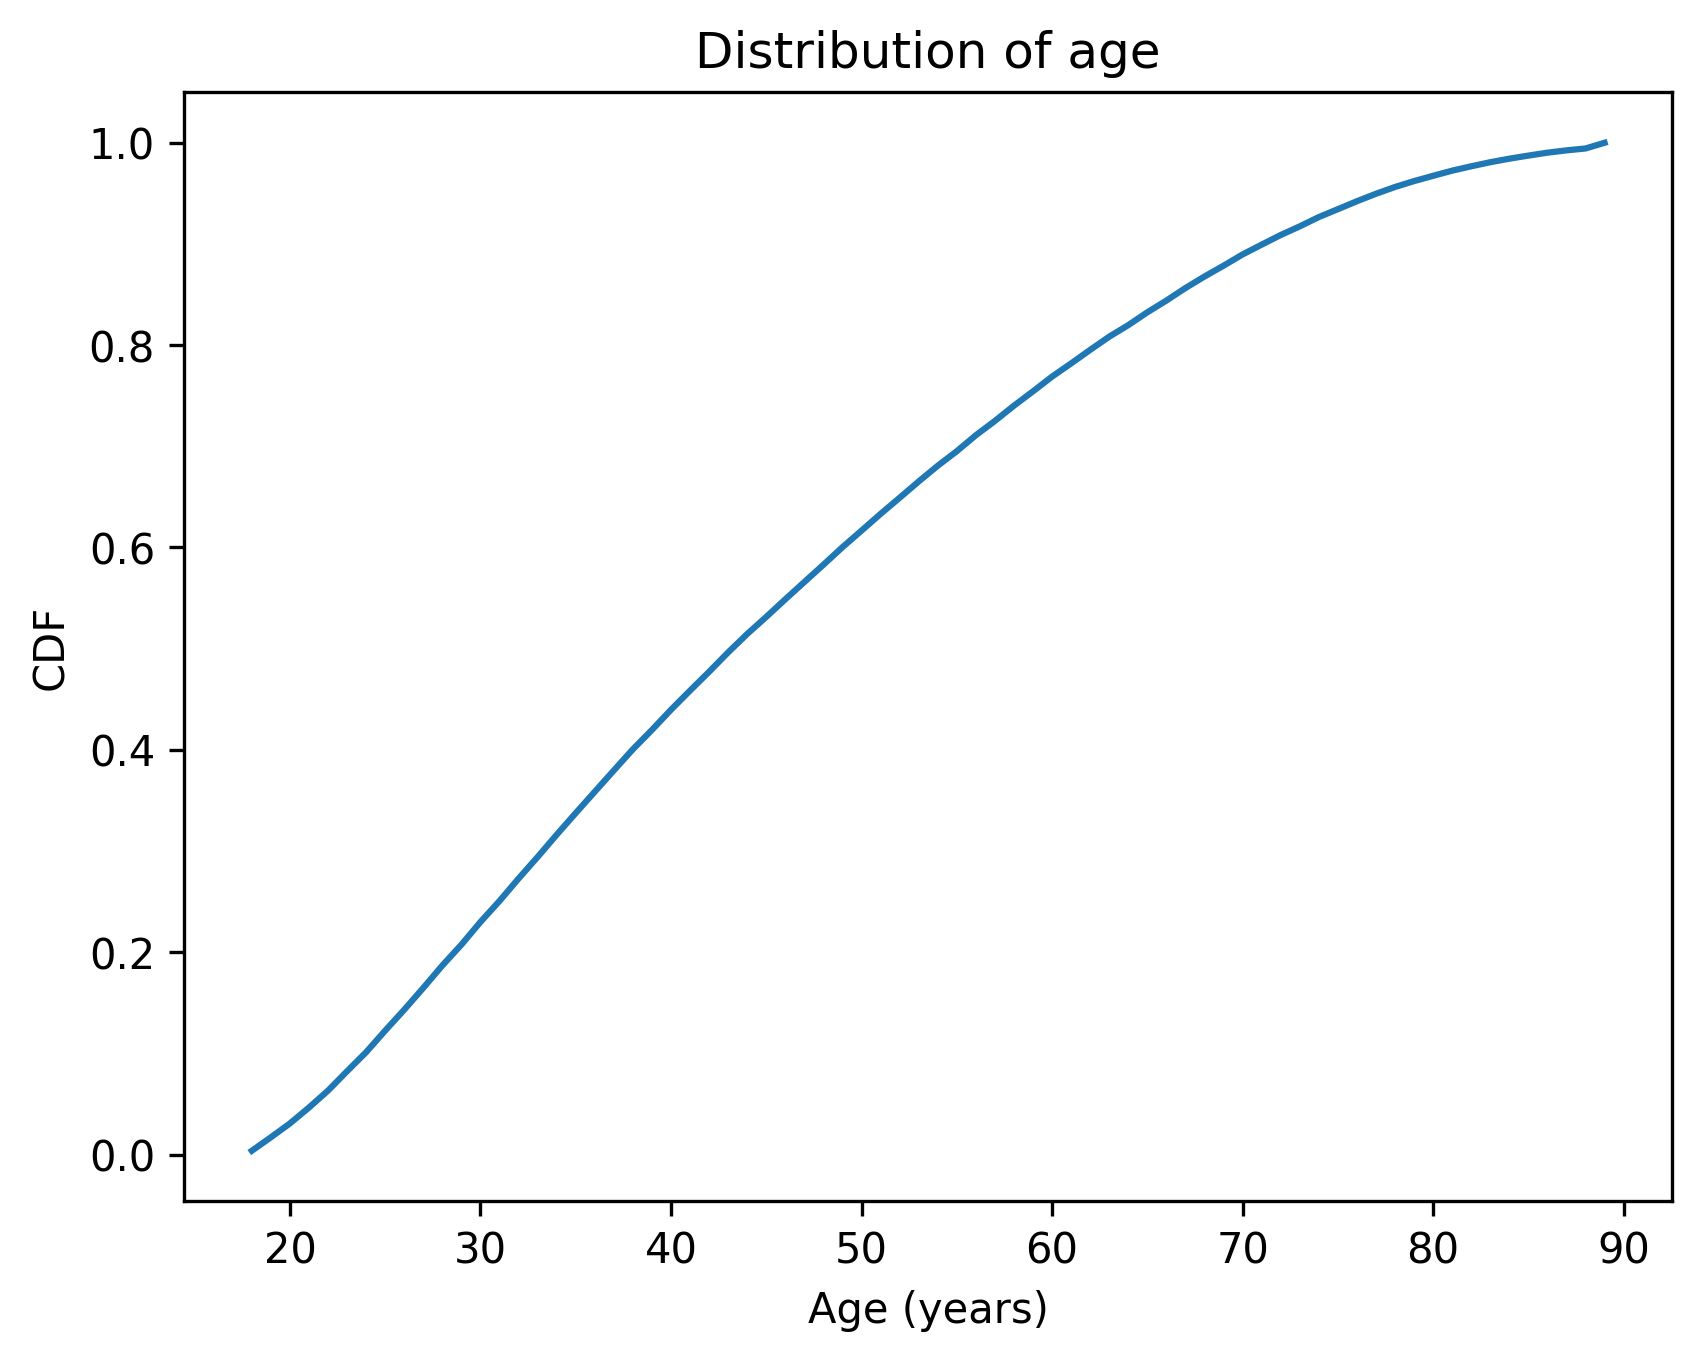
\includegraphics[width=4in]{chapters/08_distributions_files/08_distributions_66_0.png}
\end{center}

The CDF is an invertible function, which means that if you have a
probability, \passthrough{\lstinline!p!}, you can look up the
corresponding quantity, \passthrough{\lstinline!q!}.
\passthrough{\lstinline!Cdf!} provides a method called
\passthrough{\lstinline!inverse!} that computes the inverse of the
cumulative distribution function.

\begin{lstlisting}[language=Python,style=source]
p1 = 0.25
q1 = cdf_age.inverse(p1)
q1
\end{lstlisting}

\begin{lstlisting}[style=output]
array(32.)
\end{lstlisting}

In this example, we look up the probability
\passthrough{\lstinline!0.25!} and the result is
\passthrough{\lstinline!32!}.\\
That means that 25\% of the respondents are age 32 or less. Another way
to say the same thing is ``age 32 is the 25th percentile of this
distribution''.

If we look up probability \passthrough{\lstinline!0.75!}, it returns
\passthrough{\lstinline!60!}, so 75\% of the respondents are 60 or
younger.

\begin{lstlisting}[language=Python,style=source]
p2 = 0.75
q2 = cdf_age.inverse(p2)
q2
\end{lstlisting}

\begin{lstlisting}[style=output]
array(60.)
\end{lstlisting}

In the following figure, the arrows show how you could read these values
from the CDF.

\begin{lstlisting}[language=Python,style=source]
cdf_age.plot()

x = 17
draw_line(p1, q1, x)
draw_arrow_down(p1, q1, 0)

draw_line(p2, q2, x)
draw_arrow_down(p2, q2, 0)

plt.xlabel('Age (years)')
plt.xlim(x-1, 91)
plt.ylabel('CDF')
plt.title('Distribution of age');
\end{lstlisting}

\begin{center}
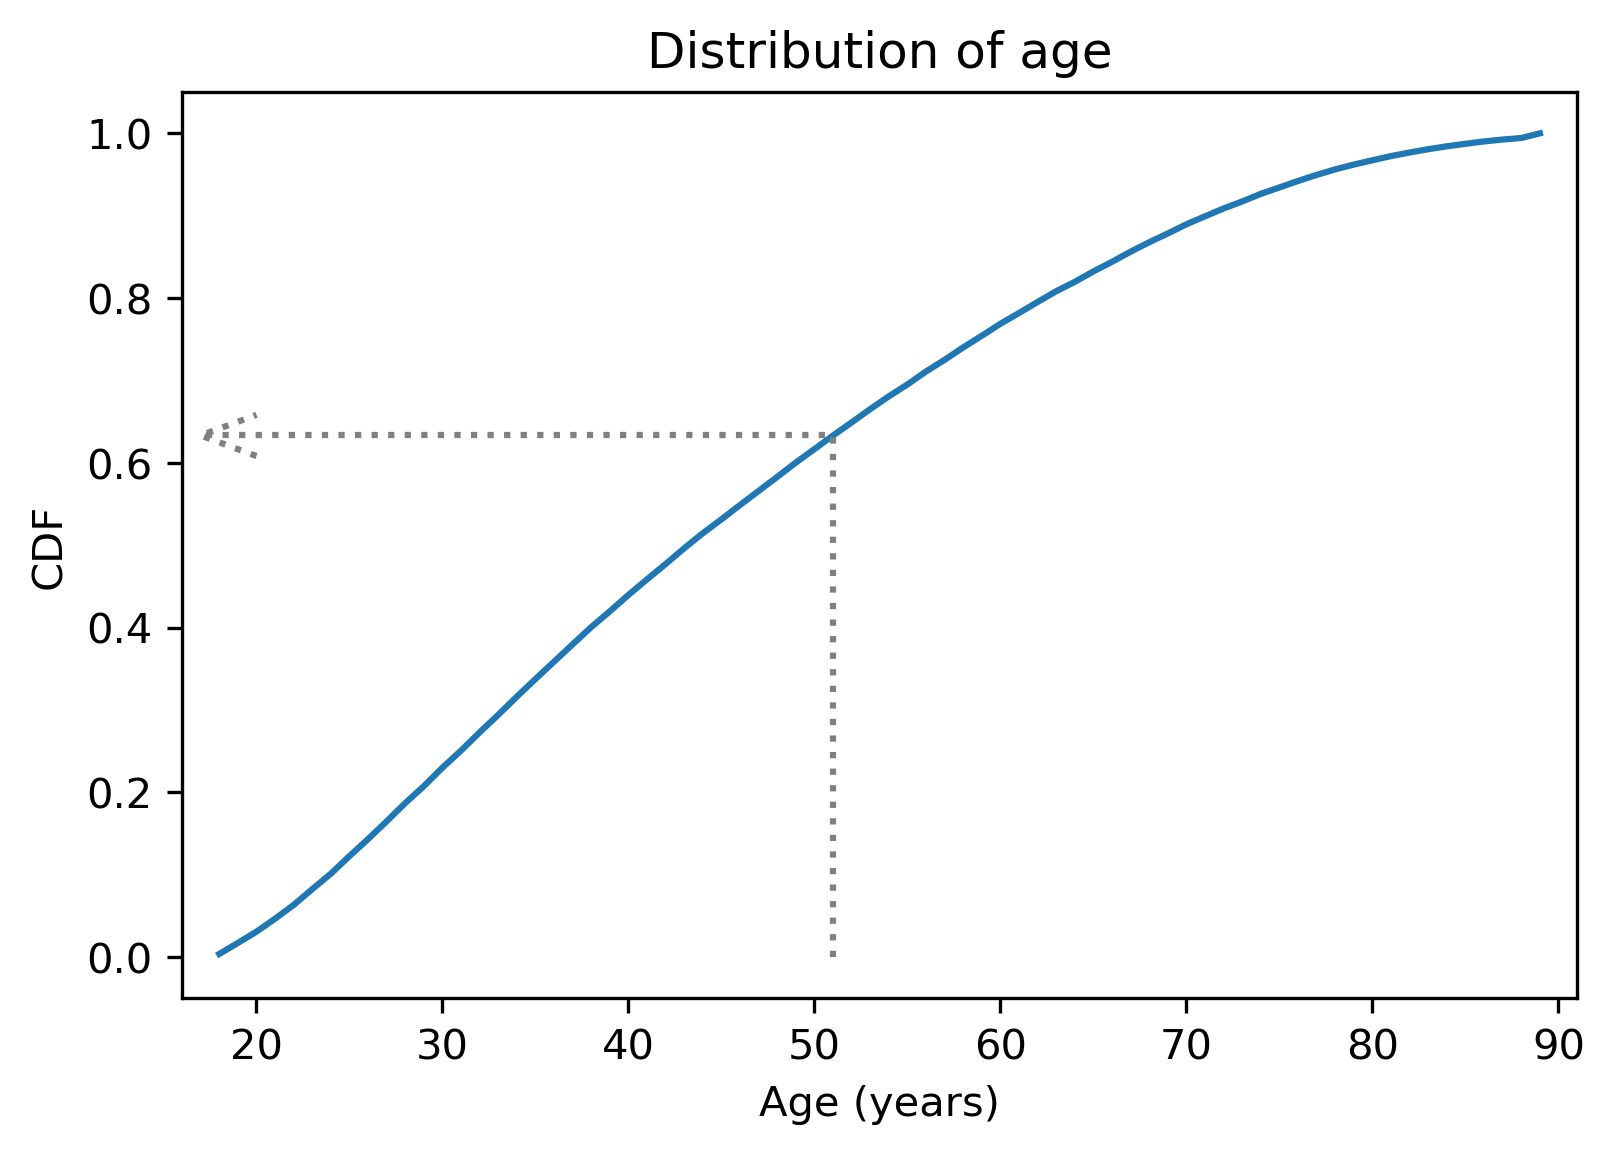
\includegraphics[width=4in]{chapters/08_distributions_files/08_distributions_72_0.png}
\end{center}

The distance from the 25th to the 75th percentile is called the
\textbf{interquartile range}, or IQR. It measures the spread of the
distribution, so it is similar to standard deviation or variance.
Because it is based on percentiles, it doesn't get thrown off by extreme
values or outliers, the way standard deviation does. So IQR is more
\textbf{robust} than variance, which means it works well even if there
are errors in the data or extreme values.

\textbf{Exercise:} Using \passthrough{\lstinline!cdf\_age!}, compute the
fraction of respondents in the GSS dataset who are \emph{older} than
\passthrough{\lstinline!65!}. Recall that the CDF computes the fraction
who are less than or equal to a value, so the complement is the fraction
who exceed a value.

\textbf{Exercise:} The distribution of income in almost every country is
long-tailed, which means there are a small number of people with very
high incomes. In the GSS dataset, the column
\passthrough{\lstinline!realinc!} represents total household income,
converted to 1986 dollars. We can get a sense of the shape of this
distribution by plotting the CDF. Select
\passthrough{\lstinline!realinc!} from the \passthrough{\lstinline!gss!}
dataset, make a \passthrough{\lstinline!Cdf!} called
\passthrough{\lstinline!cdf\_income!}, and plot it. Remember to label
the axes!

Because the tail of the distribution extends to the right, the mean is
greater than the median. Use the \passthrough{\lstinline!Cdf!} object to
compute the fraction of respondents whose income is below the mean.

\hypertarget{comparing-distributions}{%
\section{Comparing Distributions}\label{comparing-distributions}}

So far we've seen two ways to represent distributions, PMFs and CDFs.
Now we'll use PMFs and CDFs to compare distributions, and we'll see the
pros and cons of each. One way to compare distributions is to plot
multiple PMFs on the same axes. For example, suppose we want to compare
the distribution of age for male and female respondents. First we'll
create a Boolean Series that's true for male respondents and another
that's true for female respondents.

\begin{lstlisting}[language=Python,style=source]
male = (gss['sex'] == 1)
female = (gss['sex'] == 2)
\end{lstlisting}

Now we can select ages for the male and female respondents.

\begin{lstlisting}[language=Python,style=source]
male_age = age[male]
female_age = age[female]
\end{lstlisting}

And plot a PMF for each.

\begin{lstlisting}[language=Python,style=source]
pmf_male_age = Pmf.from_seq(male_age)
pmf_male_age.plot(label='Male')

pmf_female_age = Pmf.from_seq(female_age)
pmf_female_age.plot(label='Female')

plt.xlabel('Age (years)') 
plt.ylabel('PMF')
plt.title('Distribution of age by sex')
plt.legend();
\end{lstlisting}

\begin{center}
\includegraphics[width=4in]{chapters/08_distributions_files/08_distributions_81_0.png}
\end{center}

A plot like this, which is highly variable, is often described as
\textbf{noisy}. If we ignore the noise, it looks like the PMF is higher
for men between ages 40 and 50, and higher for women between ages 70 and
80. But both of those differences might be due to random variation.

Now let's do the same thing with CDFs -- everything is the same except
we replace \passthrough{\lstinline!Pmf!} with
\passthrough{\lstinline!Cdf!}.

\begin{lstlisting}[language=Python,style=source]
cdf_male_age = Cdf.from_seq(male_age)
cdf_male_age.plot(label='Male')

cdf_female_age = Cdf.from_seq(female_age)
cdf_female_age.plot(label='Female')

plt.xlabel('Age (years)') 
plt.ylabel('CDF')
plt.title('Distribution of age by sex')
plt.legend();
\end{lstlisting}

\begin{center}
\includegraphics[width=4in]{chapters/08_distributions_files/08_distributions_83_0.png}
\end{center}

In general, CDFs are smoother than PMFs. Because they smooth out
randomness, we can often get a better view of real differences between
distributions. In this case, the lines are close together until age 40
-- after that, the CDF is higher for men than women.

So what does that mean? One way to interpret the difference is that the
fraction of men below a given age is generally more than the fraction of
women below the same age. For example, about 79\% of men are
\passthrough{\lstinline!60!} or less, compared to 76\% of women.

\begin{lstlisting}[language=Python,style=source]
cdf_male_age(60), cdf_female_age(60)
\end{lstlisting}

\begin{lstlisting}[style=output]
(array(0.7721998), array(0.7474241))
\end{lstlisting}

Going the other way, we could also compare percentiles. For example, the
median age woman is older than the median age man, by about one year.

\begin{lstlisting}[language=Python,style=source]
cdf_male_age.inverse(0.5), cdf_female_age.inverse(0.5)
\end{lstlisting}

\begin{lstlisting}[style=output]
(array(44.), array(45.))
\end{lstlisting}

\textbf{Exercise:} What fraction of men are over 80? What fraction of
women?

\hypertarget{comparing-incomes}{%
\section{Comparing Incomes}\label{comparing-incomes}}

As another example, let's look at household income and compare the
distribution before and after 1995 (I chose 1995 because it's roughly
the midpoint of the survey). The column
\passthrough{\lstinline!realinc!} represents household income in 1986
dollars. We'll make two Boolean \passthrough{\lstinline!Series!} objects
to select respondents interviewed before and after 1995.

\begin{lstlisting}[language=Python,style=source]
pre95 = (gss['year'] < 1995)
post95 = (gss['year'] >= 1995)
\end{lstlisting}

Now we can plot the PMFs.

\begin{lstlisting}[language=Python,style=source]
income = gss['realinc'].replace(0, np.nan)

Pmf.from_seq(income[pre95]).plot(label='Before 1995')
Pmf.from_seq(income[post95]).plot(label='After 1995')

plt.xlabel('Income (1986 USD)')
plt.ylabel('PMF')
plt.title('Distribution of income')
plt.legend();
\end{lstlisting}

\begin{center}
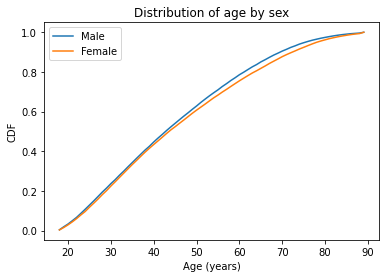
\includegraphics[width=4in]{chapters/08_distributions_files/08_distributions_92_0.png}
\end{center}

There are a lot of unique values in this distribution, and none of them
appear very often. As a result, the PMF is so noisy and we can't really
see the shape of the distribution. It's also hard to compare the
distributions. It looks like there are more people with high incomes
after 1995, but it's hard to tell. We can get a clearer picture with a
CDF.

\begin{lstlisting}[language=Python,style=source]
Cdf.from_seq(income[pre95]).plot(label='Before 1995')
Cdf.from_seq(income[post95]).plot(label='After 1995')

plt.xlabel('Income (1986 USD)')
plt.ylabel('CDF')
plt.title('Distribution of income')
plt.legend();
\end{lstlisting}

\begin{center}
\includegraphics[width=4in]{chapters/08_distributions_files/08_distributions_94_0.png}
\end{center}

Below \$30,000 the CDFs are almost identical; above that, we can see
that the post-1995 distribution is shifted to the right. In other words,
the fraction of people with high incomes is about the same, but the
income of high earners has increased.

In general, I recommend CDFs for exploratory analysis. They give you a
clear view of the distribution, without too much noise, and they are
good for comparing distributions -- especially if you have more than
two.

\textbf{Exercise:} Let's compare incomes for different levels of
education in the GSS dataset. We'll use the
\passthrough{\lstinline!degree!} column, which represents the highest
degree each respondent has earned. In this column, the value
\passthrough{\lstinline!1!} indicates a high school diploma,
\passthrough{\lstinline!2!} indicates an Associate's degree, and
\passthrough{\lstinline!3!} indicates a Bachelor's degree.

Compute and plot the distribution of income for each group. Remember to
label the CDFs, display a legend, and label the axes. Write a few
sentences that describe and interpret the results.

\hypertarget{modeling-distributions}{%
\section{Modeling Distributions}\label{modeling-distributions}}

Some distributions have names. For example, you might be familiar with
the normal distribution, also called the Gaussian distribution or the
bell curve. And you might have heard of others like the exponential
distribution, binomial distribution, or maybe Poisson distribution.
These ``distributions with names'' are called \textbf{analytic} because
they are described by analytic mathematical functions, as contrasted
with empirical distributions, which are based on data.

It turns out that many things we measure have distributions that are
well approximated by analytic distributions, so these distributions are
sometimes good models for the real world. In this context, what I mean
by a \textbf{model} is a simplified description of the world that is
accurate enough for its intended purpose. In this section, we'll compute
the CDF of a normal distribution and compare it to an empirical
distribution of data. But before we get to real data, we'll start with
fake data.

The following statement uses NumPy's \passthrough{\lstinline!random!}
library to generate 1000 values from a normal distribution with mean
\passthrough{\lstinline!0!} and standard deviation
\passthrough{\lstinline!1!}.

\begin{lstlisting}[language=Python,style=source]
sample = np.random.normal(size=1000)
\end{lstlisting}

Here's what the empirical distribution of the sample looks like.

\begin{lstlisting}[language=Python,style=source]
cdf_sample = Cdf.from_seq(sample)
cdf_sample.plot(label='Random sample')

plt.xlabel('x')
plt.ylabel('CDF')
plt.legend();
\end{lstlisting}

\begin{center}
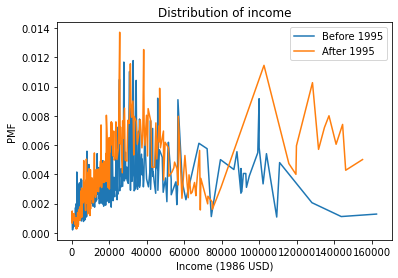
\includegraphics[width=4in]{chapters/08_distributions_files/08_distributions_102_0.png}
\end{center}

If we did not know that this sample was drawn from a normal
distribution, and we wanted to check, we could compare the CDF of the
data to the CDF of an ideal normal distribution, which we can use the
SciPy library to compute.

\begin{lstlisting}[language=Python,style=source]
from scipy.stats import norm

xs = np.linspace(-3, 3)
ys = norm(0, 1).cdf(xs)
\end{lstlisting}

First we import \passthrough{\lstinline!norm!} from
\passthrough{\lstinline!scipy.stats!}, which is a collection of
functions related to statistics. Then we use
\passthrough{\lstinline!linspace()!} to create an array of
equally-spaced points from -3 to 3; those are the
\passthrough{\lstinline!x!} values where we will evaluate the normal
CDF. Next, \passthrough{\lstinline!norm(0, 1)!} creates an object that
represents a normal distribution with mean \passthrough{\lstinline!0!}
and standard deviation \passthrough{\lstinline!1!}. Finally,
\passthrough{\lstinline!cdf!} computes the CDF of the normal
distribution, evaluated at each of the \passthrough{\lstinline!xs!}.
I'll plot the normal CDF with a gray line and then plot the CDF of the
data again.

\begin{lstlisting}[language=Python,style=source]
plt.plot(xs, ys, color='gray', label='Normal CDF')
cdf_sample.plot(label='Random sample')

plt.xlabel('x')
plt.ylabel('CDF')
plt.legend();
\end{lstlisting}

\begin{center}
\includegraphics[width=4in]{chapters/08_distributions_files/08_distributions_106_0.png}
\end{center}

The CDF of the random sample agrees with the normal model -- which is
not surprising because the data were actually sampled from a normal
distribution. When we collect data in the real world, we do not expect
it to fit a normal distribution as well as this. In the next exercise,
we'll try it and see.

\textbf{Exercise:} In many datasets, the distribution of income is
approximately \textbf{lognormal}, which means that the logarithms of the
incomes fit a normal distribution. Let's see whether that's true for the
GSS data.

\begin{itemize}
\item
  Extract \passthrough{\lstinline!realinc!} from
  \passthrough{\lstinline!gss!} and compute its logarithm using
  \passthrough{\lstinline!np.log10()!}.
\item
  Compute the mean and standard deviation of the log-transformed
  incomes.
\item
  Use \passthrough{\lstinline!norm!} to make a normal distribution with
  the same mean and standard deviation as the log-transformed incomes.
\item
  Plot the CDF of the normal distribution.
\item
  Compute and plot the CDF of the log-transformed incomes.
\end{itemize}

How similar are the CDFs of the log-transformed incomes and the normal
distribution?

\hypertarget{kernel-density-estimation}{%
\section{Kernel Density Estimation}\label{kernel-density-estimation}}

We have seen two ways to represent distributions, PMFs and CDFs. Now
we'll learn another way: a probability density function, or PDF. The
\passthrough{\lstinline!norm!} function, which we used to compute the
normal CDF, can also compute the normal PDF.

\begin{lstlisting}[language=Python,style=source]
xs = np.linspace(-3, 3)
ys = norm(0,1).pdf(xs)
plt.plot(xs, ys, color='gray', label='Normal PDF')

plt.xlabel('x')
plt.ylabel('PDF')
plt.title('Normal density function')
plt.legend();
\end{lstlisting}

\begin{center}
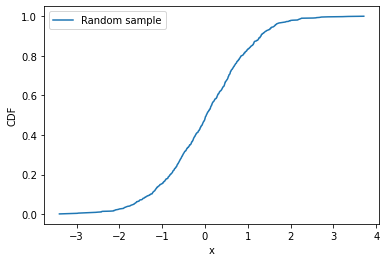
\includegraphics[width=4in]{chapters/08_distributions_files/08_distributions_112_0.png}
\end{center}

The normal PDF is the classic ``bell curve''. It is tempting to compare
the PMF of the data to the PDF of the normal distribution, but that
doesn't work. Let's see what happens if we try:

\begin{lstlisting}[language=Python,style=source]
plt.plot(xs, ys, color='gray', label='Normal PDF')

pmf_sample = Pmf.from_seq(sample)
pmf_sample.plot(label='Random sample')

plt.xlabel('x')
plt.ylabel('PDF')
plt.title('Normal density function')
plt.legend();
\end{lstlisting}

\begin{center}
\includegraphics[width=4in]{chapters/08_distributions_files/08_distributions_114_0.png}
\end{center}

The PMF of the sample is a flat line across the bottom. In the random
sample, every value is unique, so they all have the same probability,
one in 1000. However, we can use the points in the sample to estimate
the PDF of the distribution they came from. This process is called
\textbf{kernel density estimation}, or KDE. It's a way of getting from a
PMF, a probability mass function, to a PDF, a probability density
function.

To generate a KDE plot, we'll use the Seaborn library, imported as
\passthrough{\lstinline!sns!}. Seaborn provides
\passthrough{\lstinline!kdeplot!}, which takes the sample, estimates the
PDF, and plots it.

\begin{lstlisting}[language=Python,style=source]
import seaborn as sns

sns.kdeplot(sample, label='Estimated sample PDF')

plt.xlabel('x')
plt.ylabel('PDF')
plt.title('Normal density function')
plt.legend();
\end{lstlisting}

\begin{center}
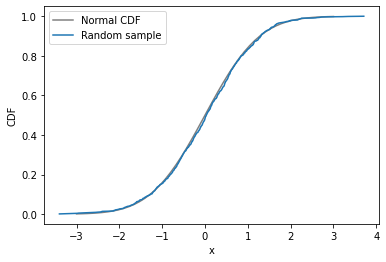
\includegraphics[width=4in]{chapters/08_distributions_files/08_distributions_116_0.png}
\end{center}

Now we can compare the KDE plot and the normal PDF.

\begin{lstlisting}[language=Python,style=source]
plt.plot(xs, ys, color='gray', label='Normal PDF')
sns.kdeplot(sample, label='Estimated sample PDF')

plt.xlabel('x')
plt.ylabel('PDF')
plt.title('Normal density function')
plt.legend();
\end{lstlisting}

\begin{center}
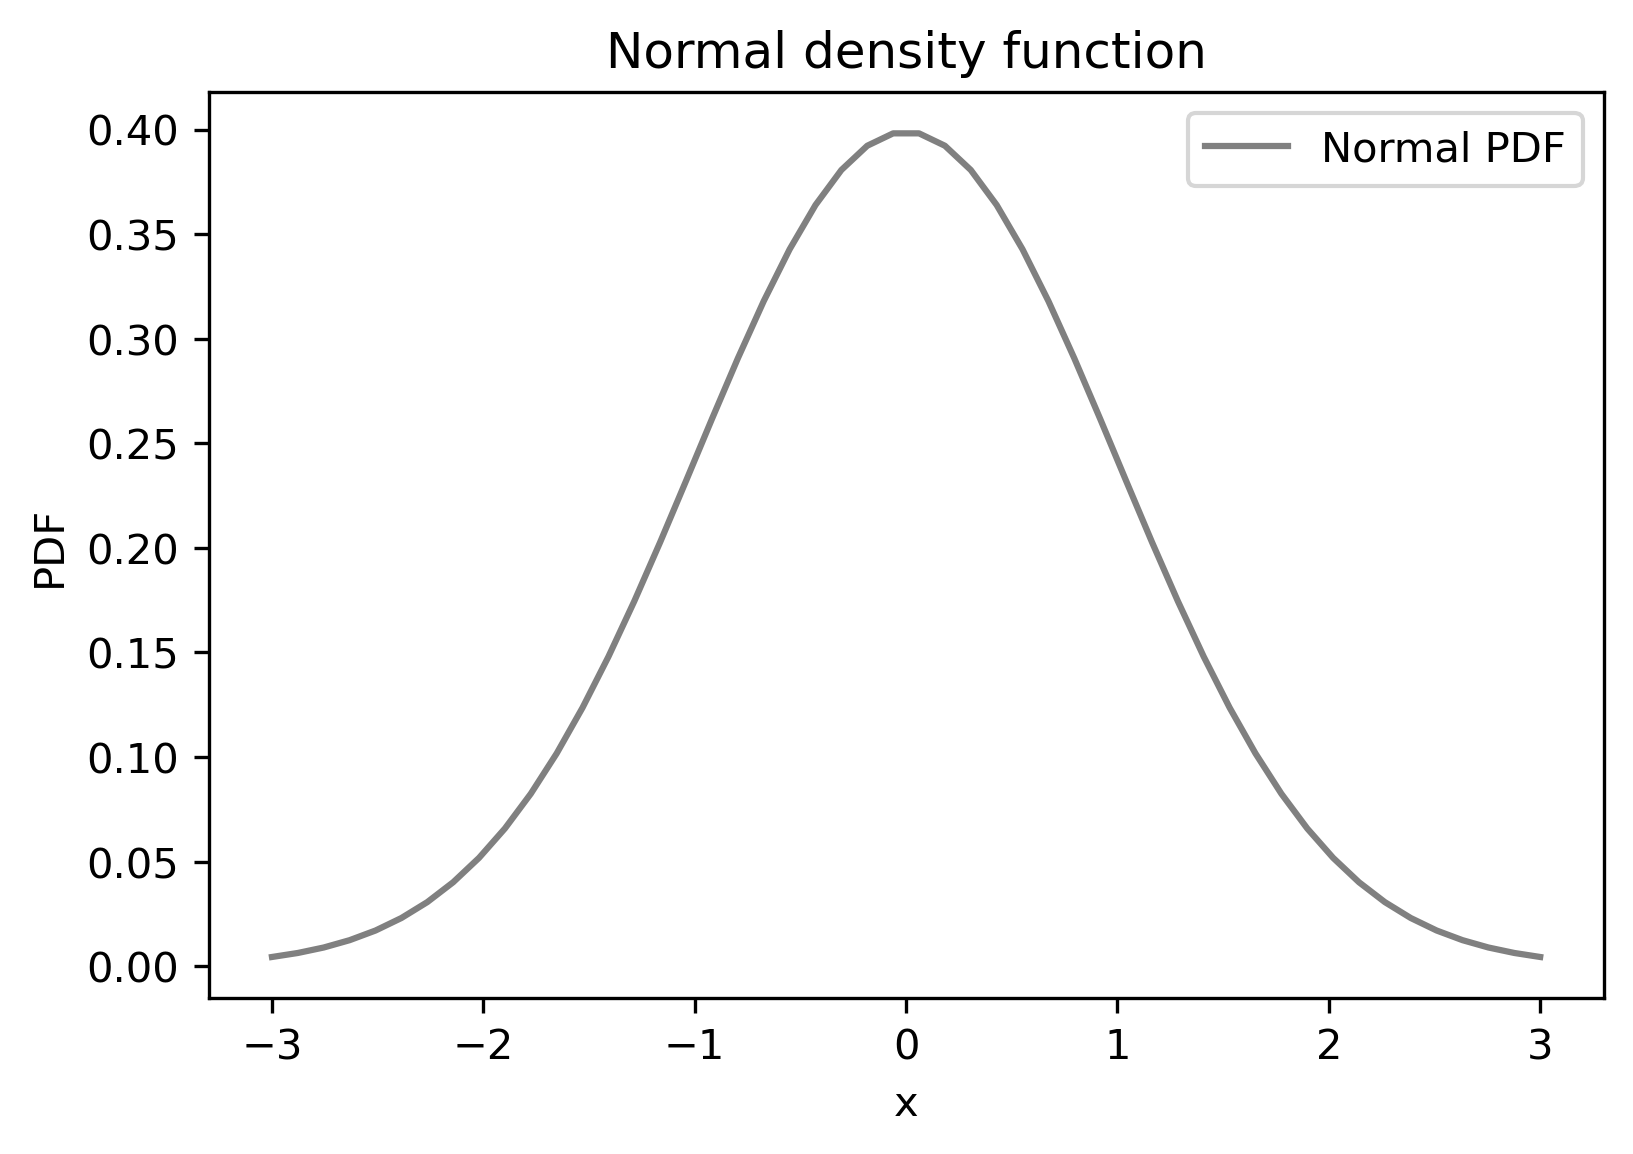
\includegraphics[width=4in]{chapters/08_distributions_files/08_distributions_118_0.png}
\end{center}

The KDE plot matches the normal PDF pretty well, although the
differences look bigger when we compare PDFs than they did with the
CDFs. That means that the PDF is a more sensitive way to look for
differences, but often it is too sensitive.\\
It's hard to tell whether apparent differences mean anything, or if they
are just random, as in this case.

\textbf{Exercise:} In a previous exercise, we used CDFs to see if the
distribution of income fits a lognormal distribution. We can make the
same comparison using a PDF and KDE.

\begin{itemize}
\item
  Again, extract \passthrough{\lstinline!realinc!} from
  \passthrough{\lstinline!gss!} and compute its logarithm using
  \passthrough{\lstinline!np.log10()!}.
\item
  Compute the mean and standard deviation of the log-transformed
  incomes.
\item
  Use \passthrough{\lstinline!norm!} to make a normal distribution with
  the same mean and standard deviation as the log-transformed incomes.
\item
  Plot the PDF of the normal distribution.
\item
  Use \passthrough{\lstinline!sns.kdeplot()!} to estimate and plot the
  density of the log-transformed incomes.
\end{itemize}

\hypertarget{summary}{%
\section{Summary}\label{summary}}

In this chapter, we've seen four ways to visualize distributions, PMFs,
CDFs, and KDE plots. In general, I use CDFs when I am exploring data.
That way, I get the best view of what's going on without getting
distracted by noise. Then, if I am presenting results to an audience
unfamiliar with CDFs, I might use a PMF if the dataset contains a small
number of unique values, or KDE if there are many unique values.



\hypertarget{relationships}{%
\chapter{Relationships}\label{relationships}}

This chapter explores relationships between variables.

\begin{itemize}
\item
  We will visualize relationships using scatter plots, box plots, and
  violin plots,
\item
  And we will quantify relationships using correlation and simple
  regression.
\end{itemize}

The most important lesson in this chapter is that you should always
visualize the relationship between variables before you try to quantify
it; otherwise, you are likely to be misled.

\hypertarget{exploring-relationships}{%
\section{Exploring relationships}\label{exploring-relationships}}

So far we have mostly considered one variable at a time. Now it's time
to explore relationships between variables. As a first example, we'll
look at the relationship between height and weight.

We'll use data from the Behavioral Risk Factor Surveillance System
(BRFSS), which is run by the Centers for Disease Control at
\url{https://www.cdc.gov/brfss}. The survey includes more than 400,000
respondents, but to keep things manageable, we'll work with a random
subsample of 100,000.

\begin{lstlisting}[]
import pandas as pd

brfss = pd.read_hdf('brfss.hdf5', 'brfss')
brfss.shape
(@\dashfill@)
@@@(100000, 9)@@@
\end{lstlisting}

Here are the first few rows.

\begin{lstlisting}[]
brfss.head()
(@\dashfill@)
@@@/home/downey/miniconda3/envs/ElementsOfDataScience/lib/python3.8/site-packages/IPython/core/formatters.py:342: FutureWarning: In future versions `DataFrame.to_latex` is expected to utilise the base implementation of `Styler.to_latex` for formatting and rendering. The arguments signature may therefore change. It is recommended instead to use `DataFrame.style.to_latex` which also contains additional functionality.
  return method()@@@
\end{lstlisting}

\begin{tabular}{lrrrrrrrrr}
\midrule
{} &  SEX &   HTM4 &   WTKG3 &  INCOME2 &       \_LLCPWT &  \_AGEG5YR &  \_VEGESU1 &  \_HTMG10 &   AGE \\
\midrule
96230  &  2.0 &  160.0 &   60.33 &      8.0 &   1398.525290 &       6.0 &      2.14 &    150.0 &  47.0 \\
244920 &  2.0 &  163.0 &   58.97 &      5.0 &     84.057503 &      13.0 &      3.14 &    160.0 &  89.5 \\
57312  &  2.0 &  163.0 &   72.57 &      8.0 &    390.248599 &       5.0 &      2.64 &    160.0 &  42.0 \\
32573  &  2.0 &  165.0 &   74.84 &      1.0 &  11566.705300 &       3.0 &      1.46 &    160.0 &  32.0 \\
355929 &  2.0 &  170.0 &  108.86 &      3.0 &    844.485450 &       3.0 &      1.81 &    160.0 &  32.0 \\
\midrule
\end{tabular}

The BRFSS includes hundreds of variables. For the examples in this
chapter, we'll work with just nine. The ones we'll start with are
\passthrough{\lstinline!HTM4!}, which records each respondent's height
in cm, and \passthrough{\lstinline!WTKG3!}, which records weight in kg.

\begin{lstlisting}[]
height = brfss['HTM4']
weight = brfss['WTKG3']
\end{lstlisting}

To visualize the relationship between these variables, we'll make a
\textbf{scatter plot}, which shows one marker for each pair of values.
Scatter plots are common and readily understood, but they are
surprisingly hard to get right.

As a first attempt, we'll use \passthrough{\lstinline!plot!} with the
style string \passthrough{\lstinline!o!}, which plots a circle for each
data point.

\begin{lstlisting}[]
import matplotlib.pyplot as plt

plt.plot(height, weight, 'o')

plt.xlabel('Height in cm')
plt.ylabel('Weight in kg')
plt.title('Scatter plot of weight versus height');
\end{lstlisting}

\begin{center}
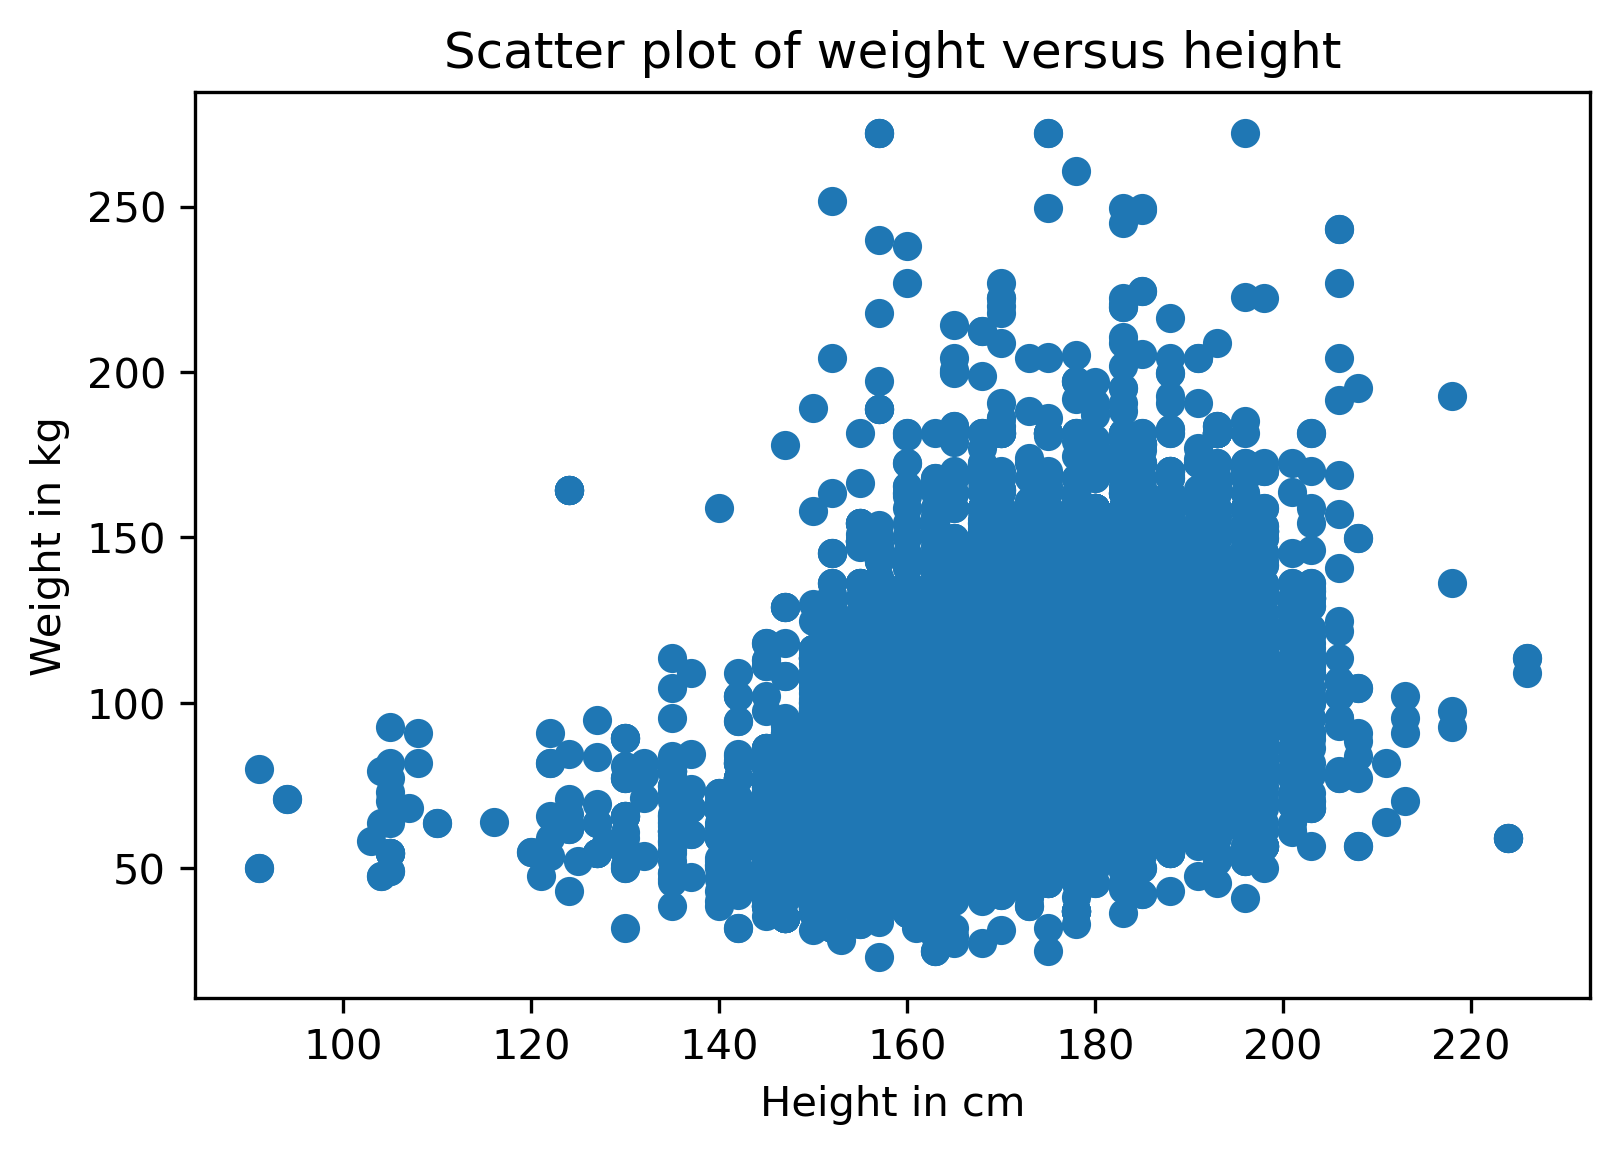
\includegraphics[width=4in]{chapters/09_relationships_files/09_relationships_12_0.png}
\end{center}

Each marker represents the height and weight of one person.

Based on the shape of the result, it looks like taller people are
heavier, but there are a few things about this plot that make it hard to
interpret. Most importantly, it is \textbf{overplotted}, which means
that there are markers piled on top of each other so you can't tell
where there are a lot of data points and where there is just one. When
that happens, the results can be seriously misleading.

One way to improve the plot is to use transparency, which we can do with
the keyword argument \passthrough{\lstinline!alpha!}. The lower the
value of alpha, the more transparent each data point is.

Here's what it looks like with \passthrough{\lstinline!alpha=0.02!}.

\begin{lstlisting}[]
plt.plot(height, weight, 'o', alpha=0.02)

plt.xlabel('Height in cm')
plt.ylabel('Weight in kg')
plt.title('Scatter plot of weight versus height');
\end{lstlisting}

\begin{center}
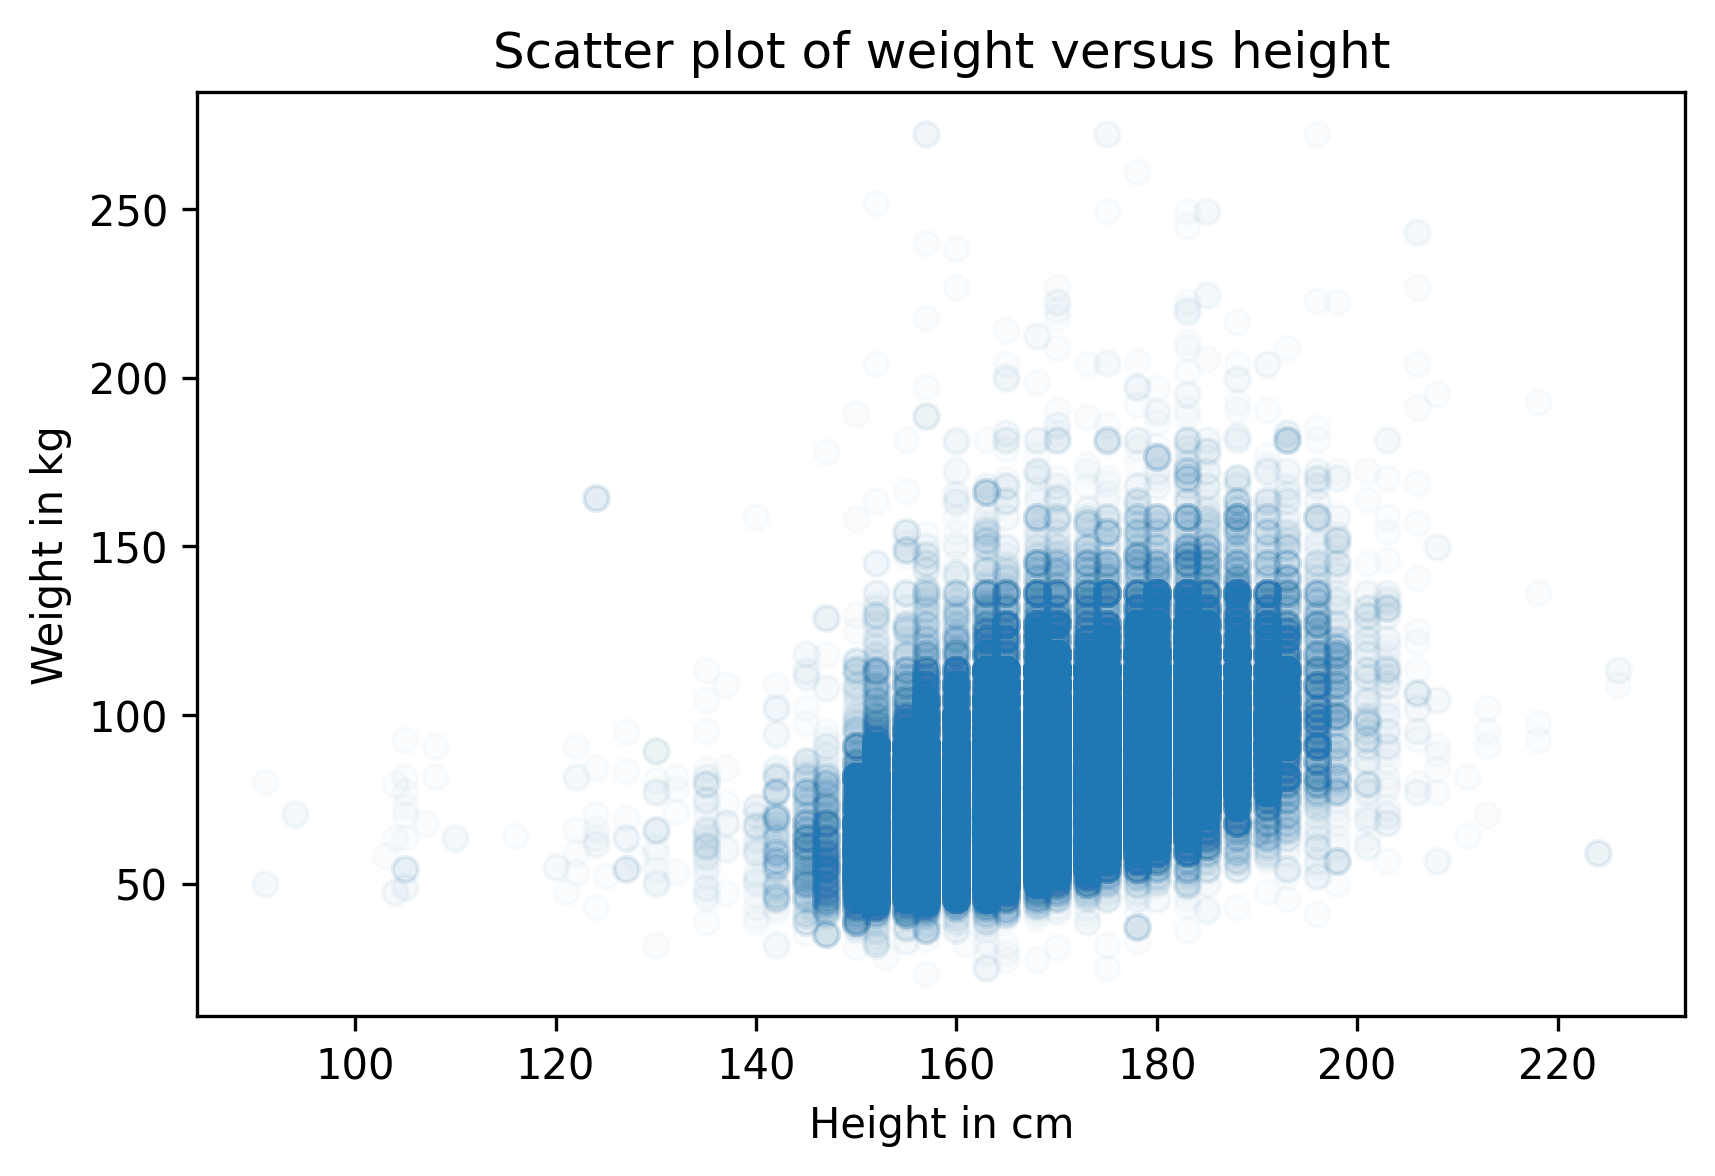
\includegraphics[width=4in]{chapters/09_relationships_files/09_relationships_14_0.png}
\end{center}

This is better, but there are so many data points, the scatter plot is
still overplotted. The next step is to make the markers smaller. With
\passthrough{\lstinline!markersize=1!} and a low value of alpha, the
scatter plot is less saturated. Here's what it looks like.

\begin{lstlisting}[]
plt.plot(height, weight, 'o', alpha=0.02, markersize=1)

plt.xlabel('Height in cm')
plt.ylabel('Weight in kg')
plt.title('Scatter plot of weight versus height');
\end{lstlisting}

\begin{center}
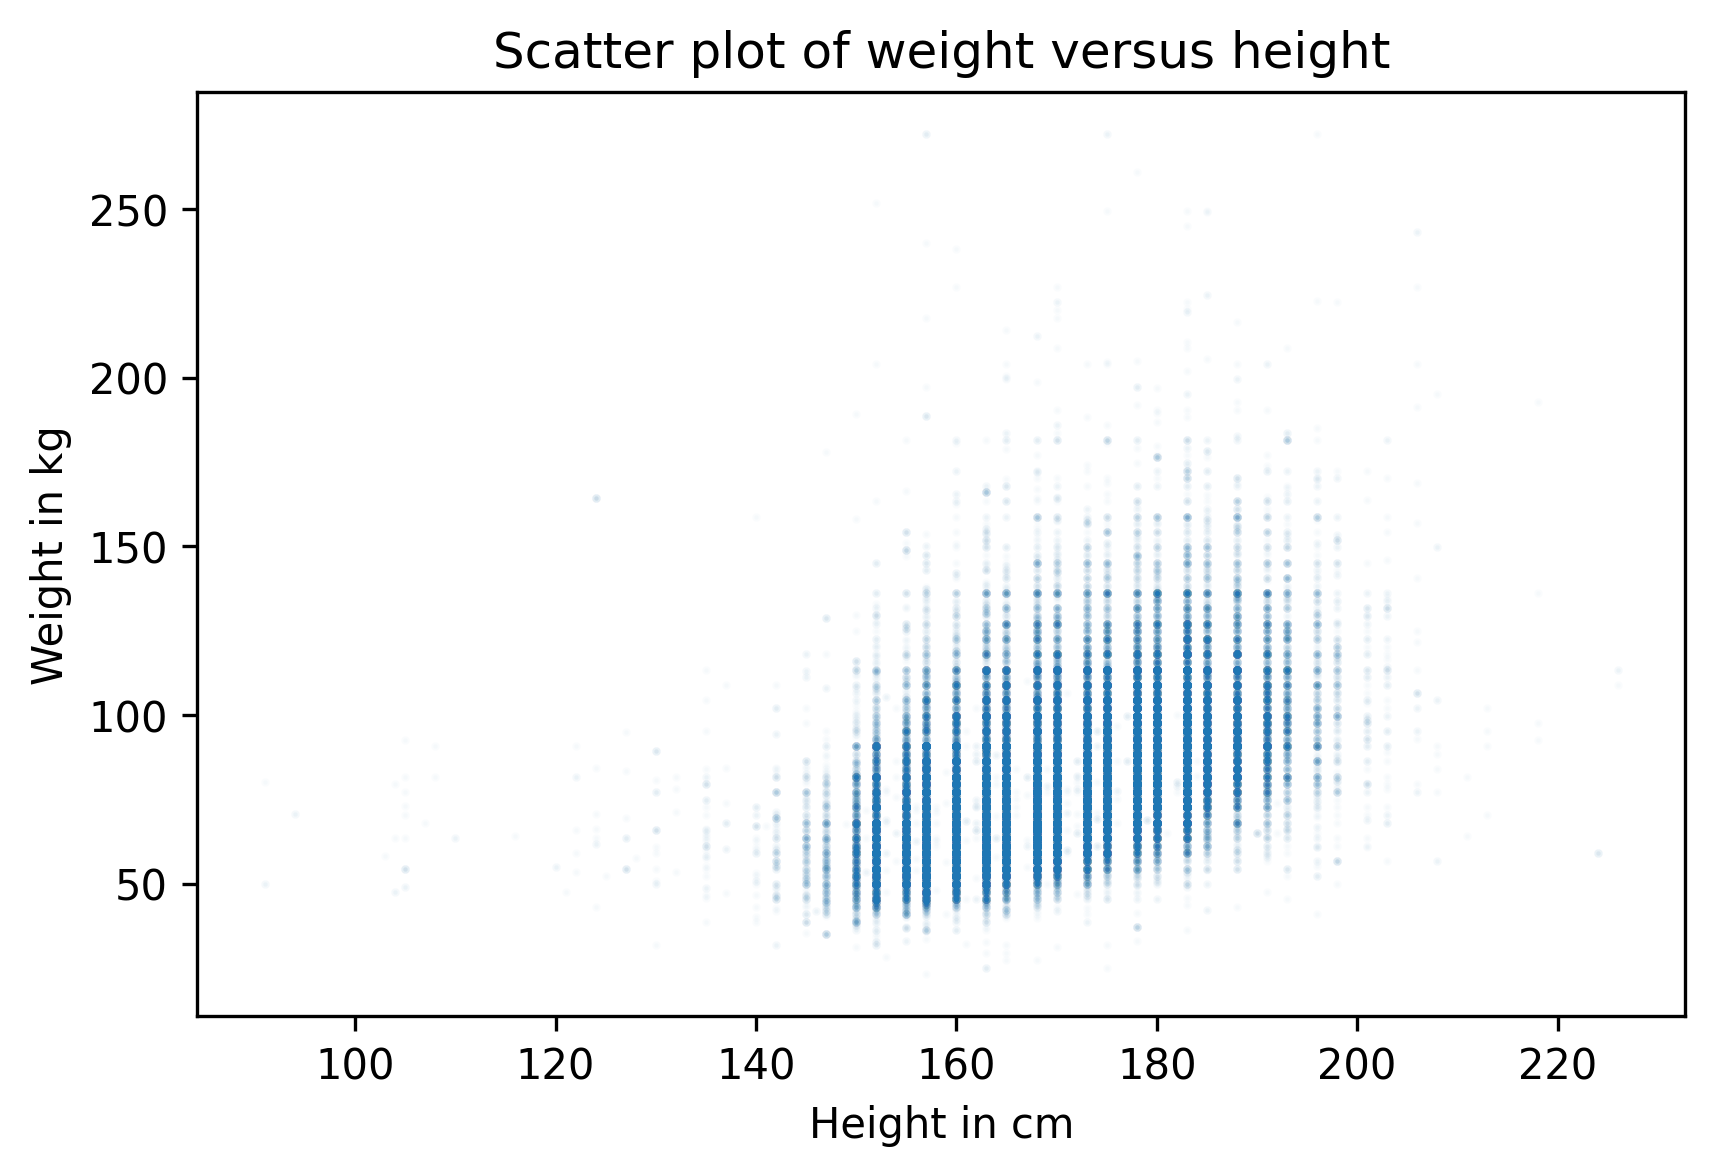
\includegraphics[width=4in]{chapters/09_relationships_files/09_relationships_16_0.png}
\end{center}

Again, this is better, but now we can see that the points fall in
discrete columns. That's because most heights were reported in inches
and converted to centimeters. We can break up the columns by adding some
random noise to the values; in effect, we are filling in the values that
got rounded off. Adding random noise like this is called
\textbf{jittering}.

We can use NumPy to add noise from a normal distribution with mean 0 and
standard deviation 2.

\begin{lstlisting}[]
import numpy as np

noise = np.random.normal(0, 2, size=len(brfss))
height_jitter = height + noise
\end{lstlisting}

Here's what the plot looks like with jittered heights.

\begin{lstlisting}[]
plt.plot(height_jitter, weight, 'o', 
         alpha=0.02, markersize=1)

plt.xlabel('Height in cm')
plt.ylabel('Weight in kg')
plt.title('Scatter plot of weight versus height');
\end{lstlisting}

\begin{center}
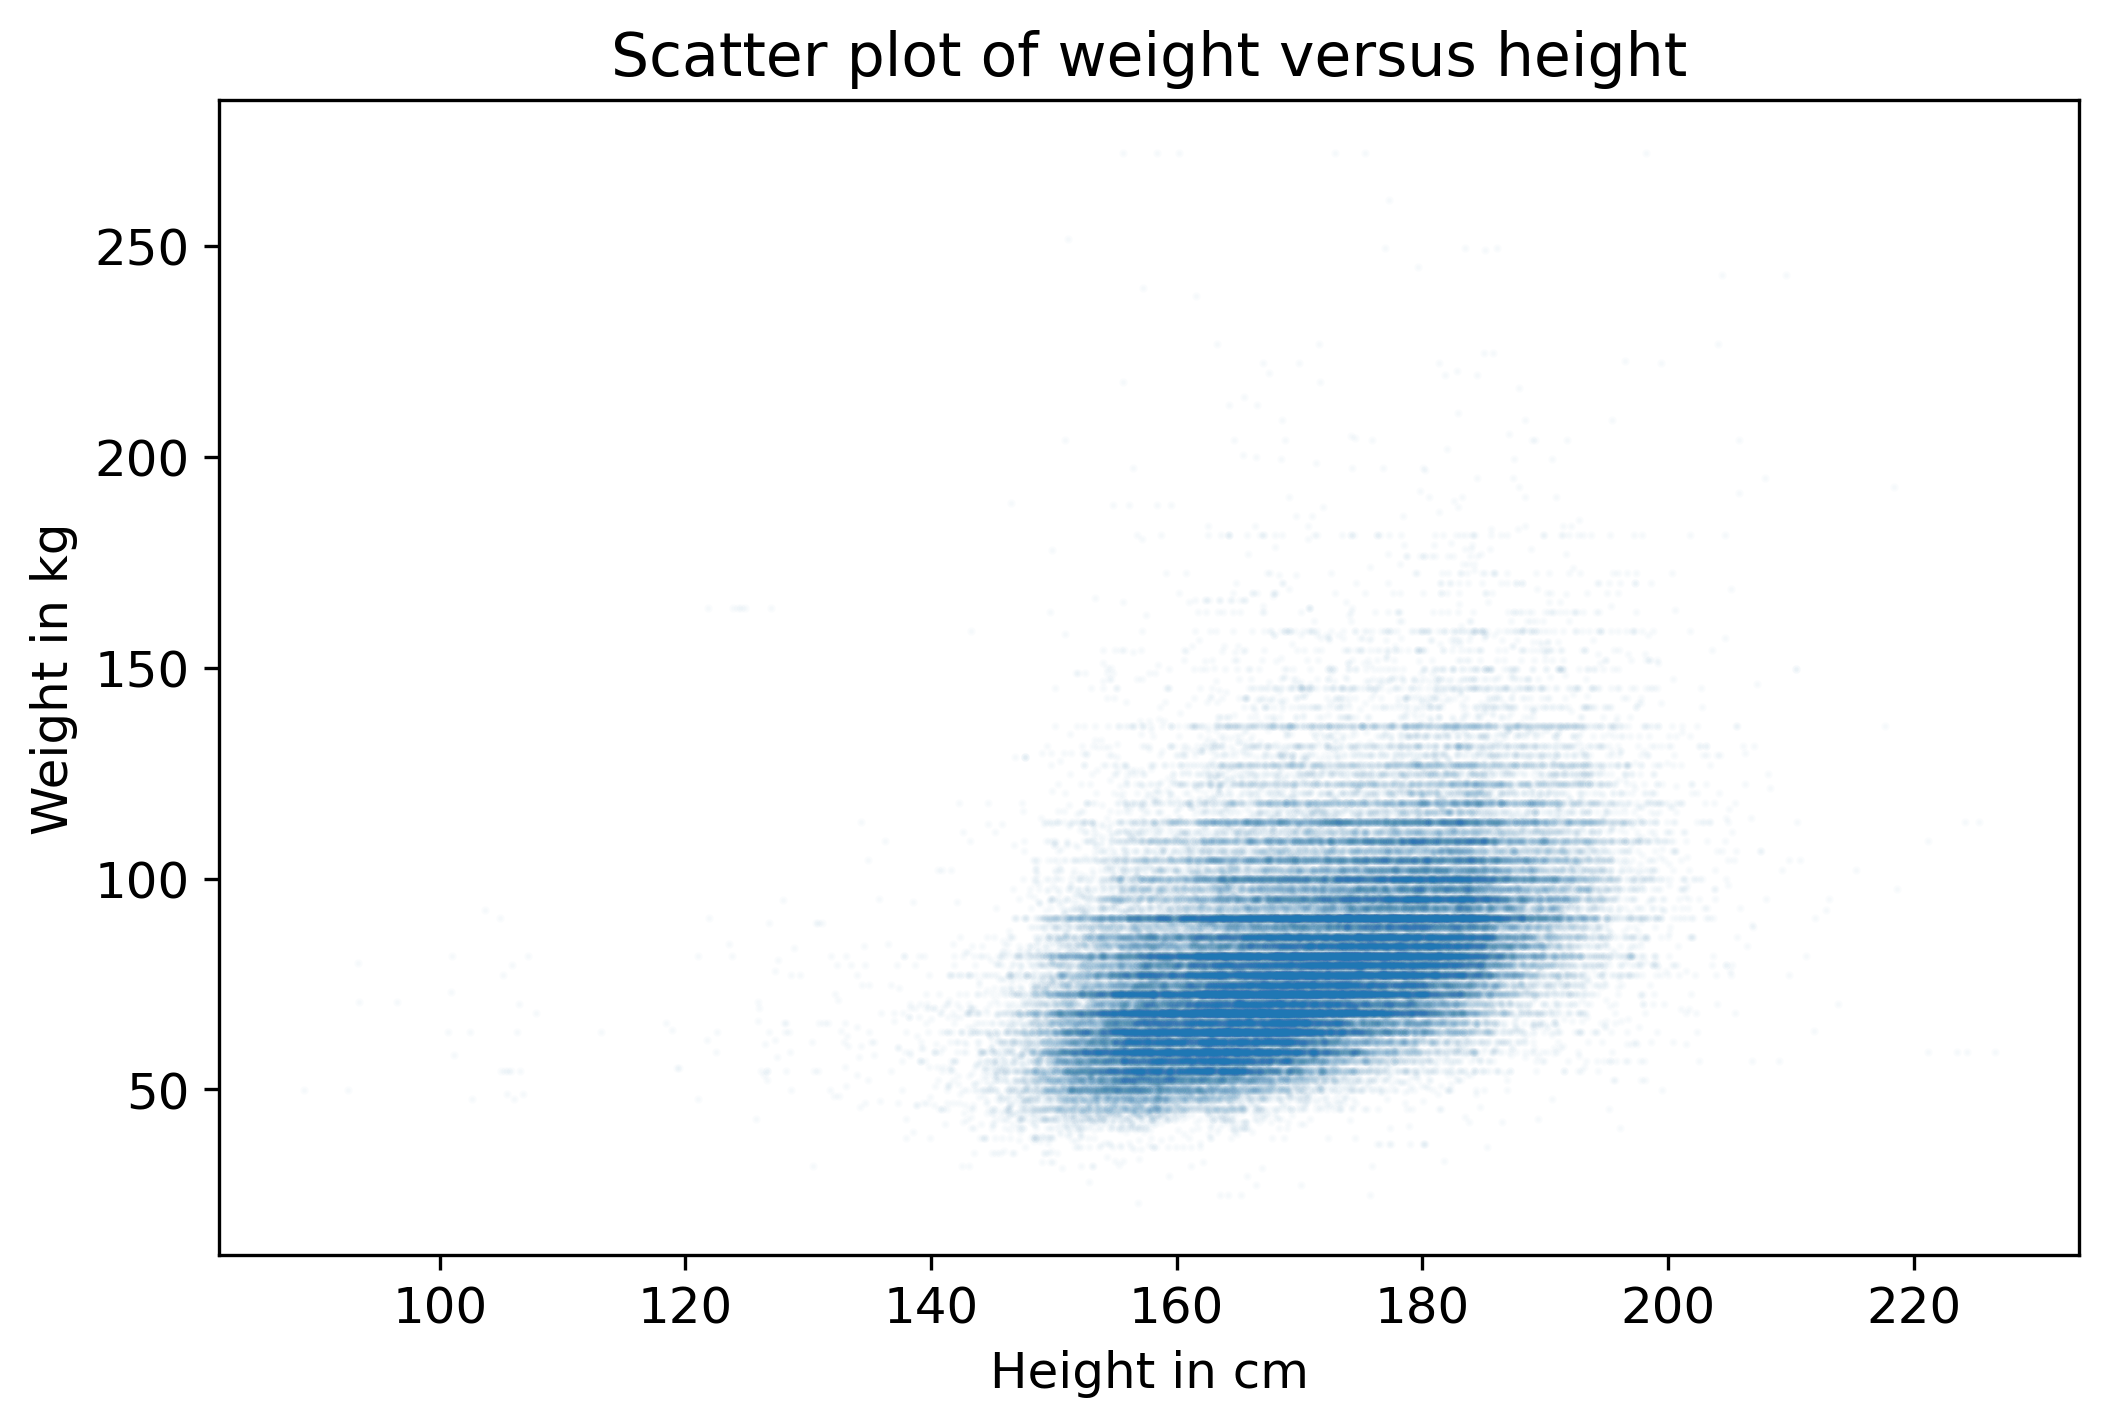
\includegraphics[width=4in]{chapters/09_relationships_files/09_relationships_20_0.png}
\end{center}

The columns are gone, but now we can see that there are rows where
people rounded off their weight. We can fix that by jittering weight,
too.

\begin{lstlisting}[]
noise = np.random.normal(0, 2, size=len(brfss))
weight_jitter = weight + noise
\end{lstlisting}

\begin{lstlisting}[]
plt.plot(height_jitter, weight_jitter, 'o', 
         alpha=0.02, markersize=1)

plt.xlabel('Height in cm')
plt.ylabel('Weight in kg')
plt.title('Scatter plot of weight versus height');
\end{lstlisting}

\begin{center}
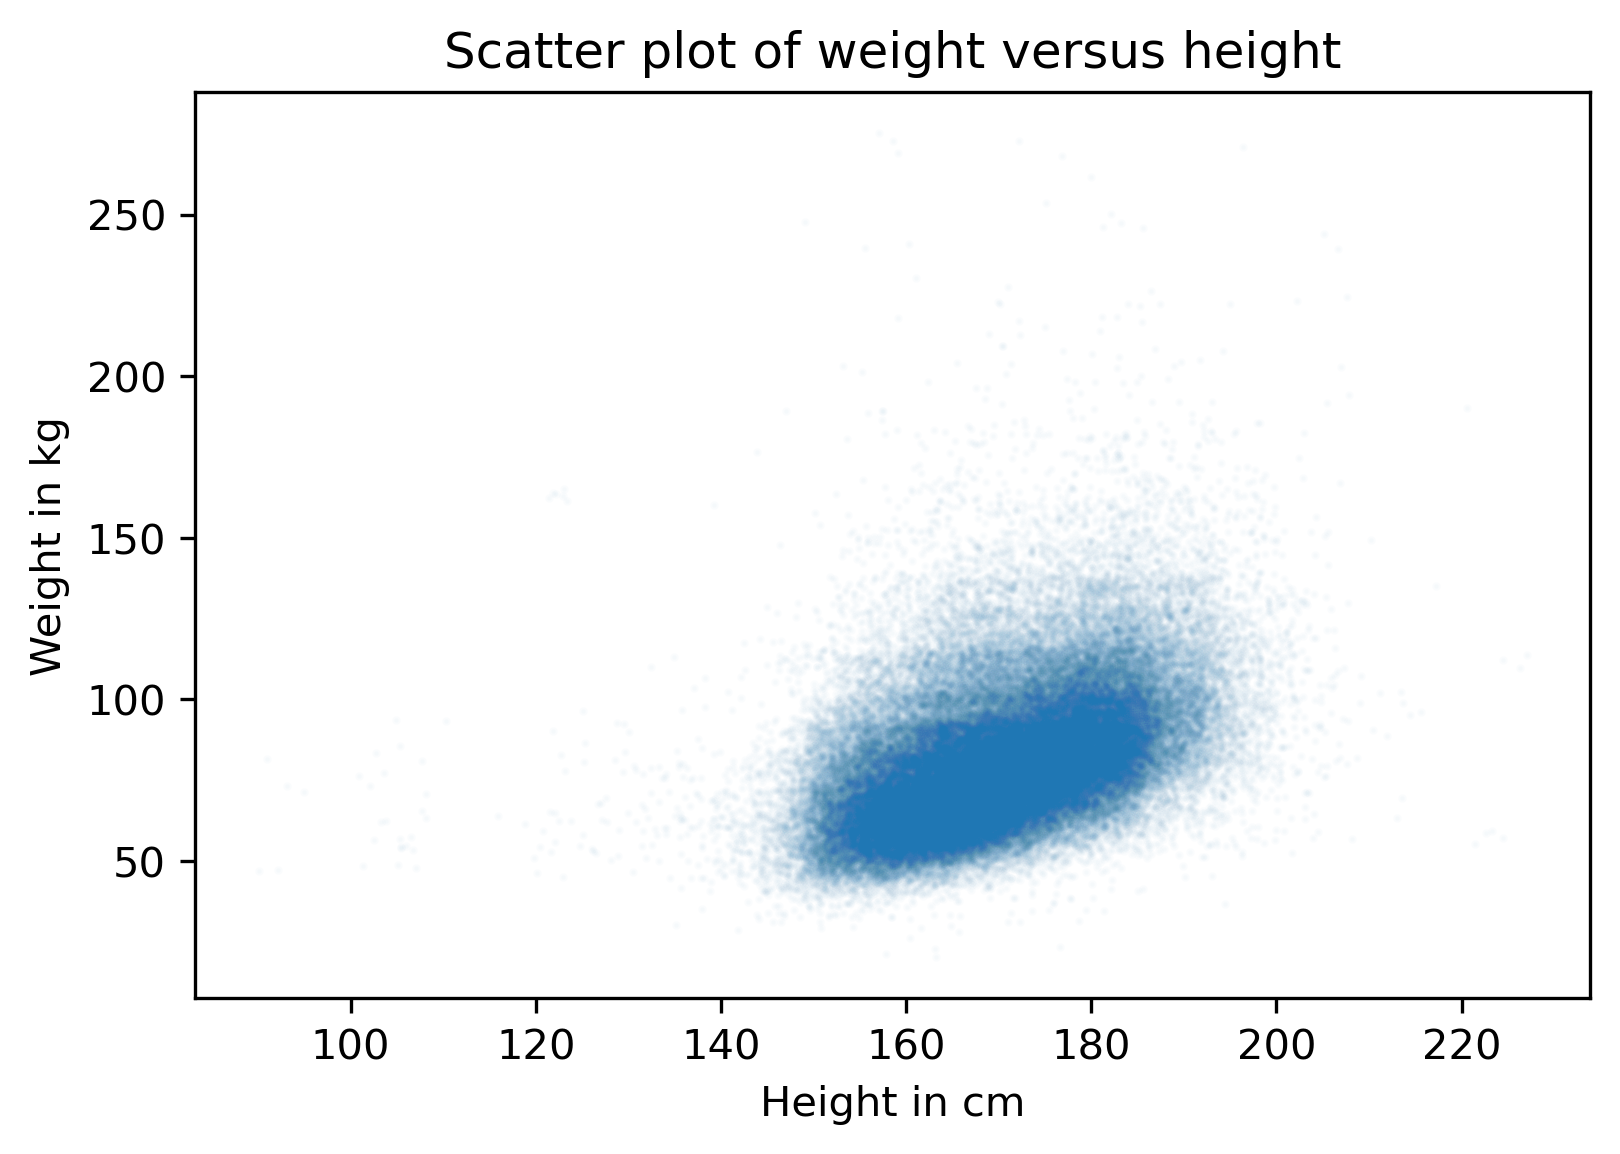
\includegraphics[width=4in]{chapters/09_relationships_files/09_relationships_23_0.png}
\end{center}

Finally, let's zoom in on the area where most of the data points are.

The functions \passthrough{\lstinline!xlim!} and
\passthrough{\lstinline!ylim!} set the lower and upper bounds for the
\(x\) and \(y\)-axis; in this case, we plot heights from 140 to 200
centimeters and weights up to 160 kilograms.

Here's what it looks like.

\begin{lstlisting}[]
plt.plot(height_jitter, weight_jitter, 'o', 
         alpha=0.02, markersize=1)

plt.xlim([140, 200])
plt.ylim([0, 160])
plt.xlabel('Height in cm')
plt.ylabel('Weight in kg')
plt.title('Scatter plot of weight versus height');
\end{lstlisting}

\begin{center}
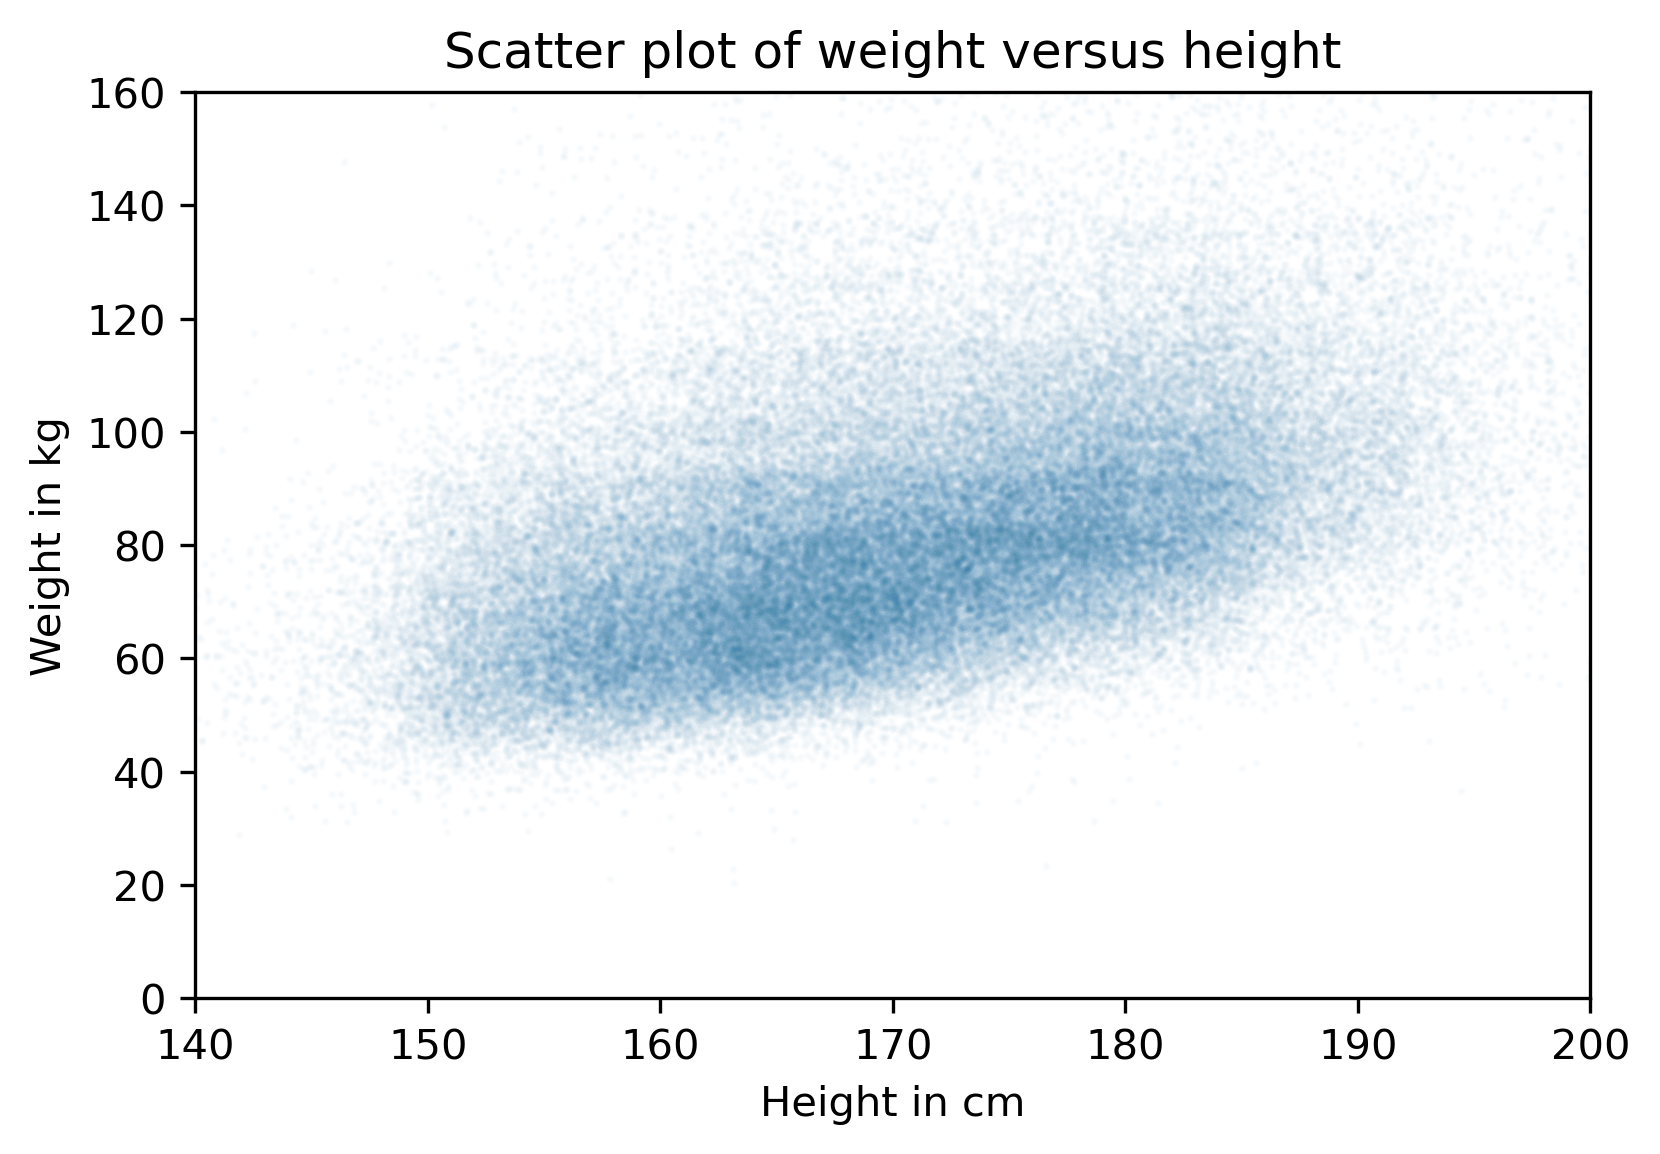
\includegraphics[width=4in]{chapters/09_relationships_files/09_relationships_25_0.png}
\end{center}

Now we have a reliable picture of the relationship between height and
weight.

Below you can see the misleading plot we started with and the more
reliable one we ended with. They are clearly different, and they suggest
different relationships between these variables.

\begin{lstlisting}[]
# Set the figure size
plt.figure(figsize=(8, 3))

# Create subplots with 2 rows, 1 column, and start plot 1
plt.subplot(1, 2, 1)
plt.plot(height, weight, 'o')

plt.xlabel('Height in cm')
plt.ylabel('Weight in kg')
plt.title('Scatter plot of weight versus height')

# Adjust the layout so the two plots don't overlap
plt.tight_layout()

# Start plot 2
plt.subplot(1, 2, 2)

plt.plot(height_jitter, weight_jitter, 'o', 
         alpha=0.02, markersize=1)

plt.xlim([140, 200])
plt.ylim([0, 160])
plt.xlabel('Height in cm')
plt.ylabel('Weight in kg')
plt.title('Scatter plot of weight versus height')
plt.tight_layout()
\end{lstlisting}

\begin{center}
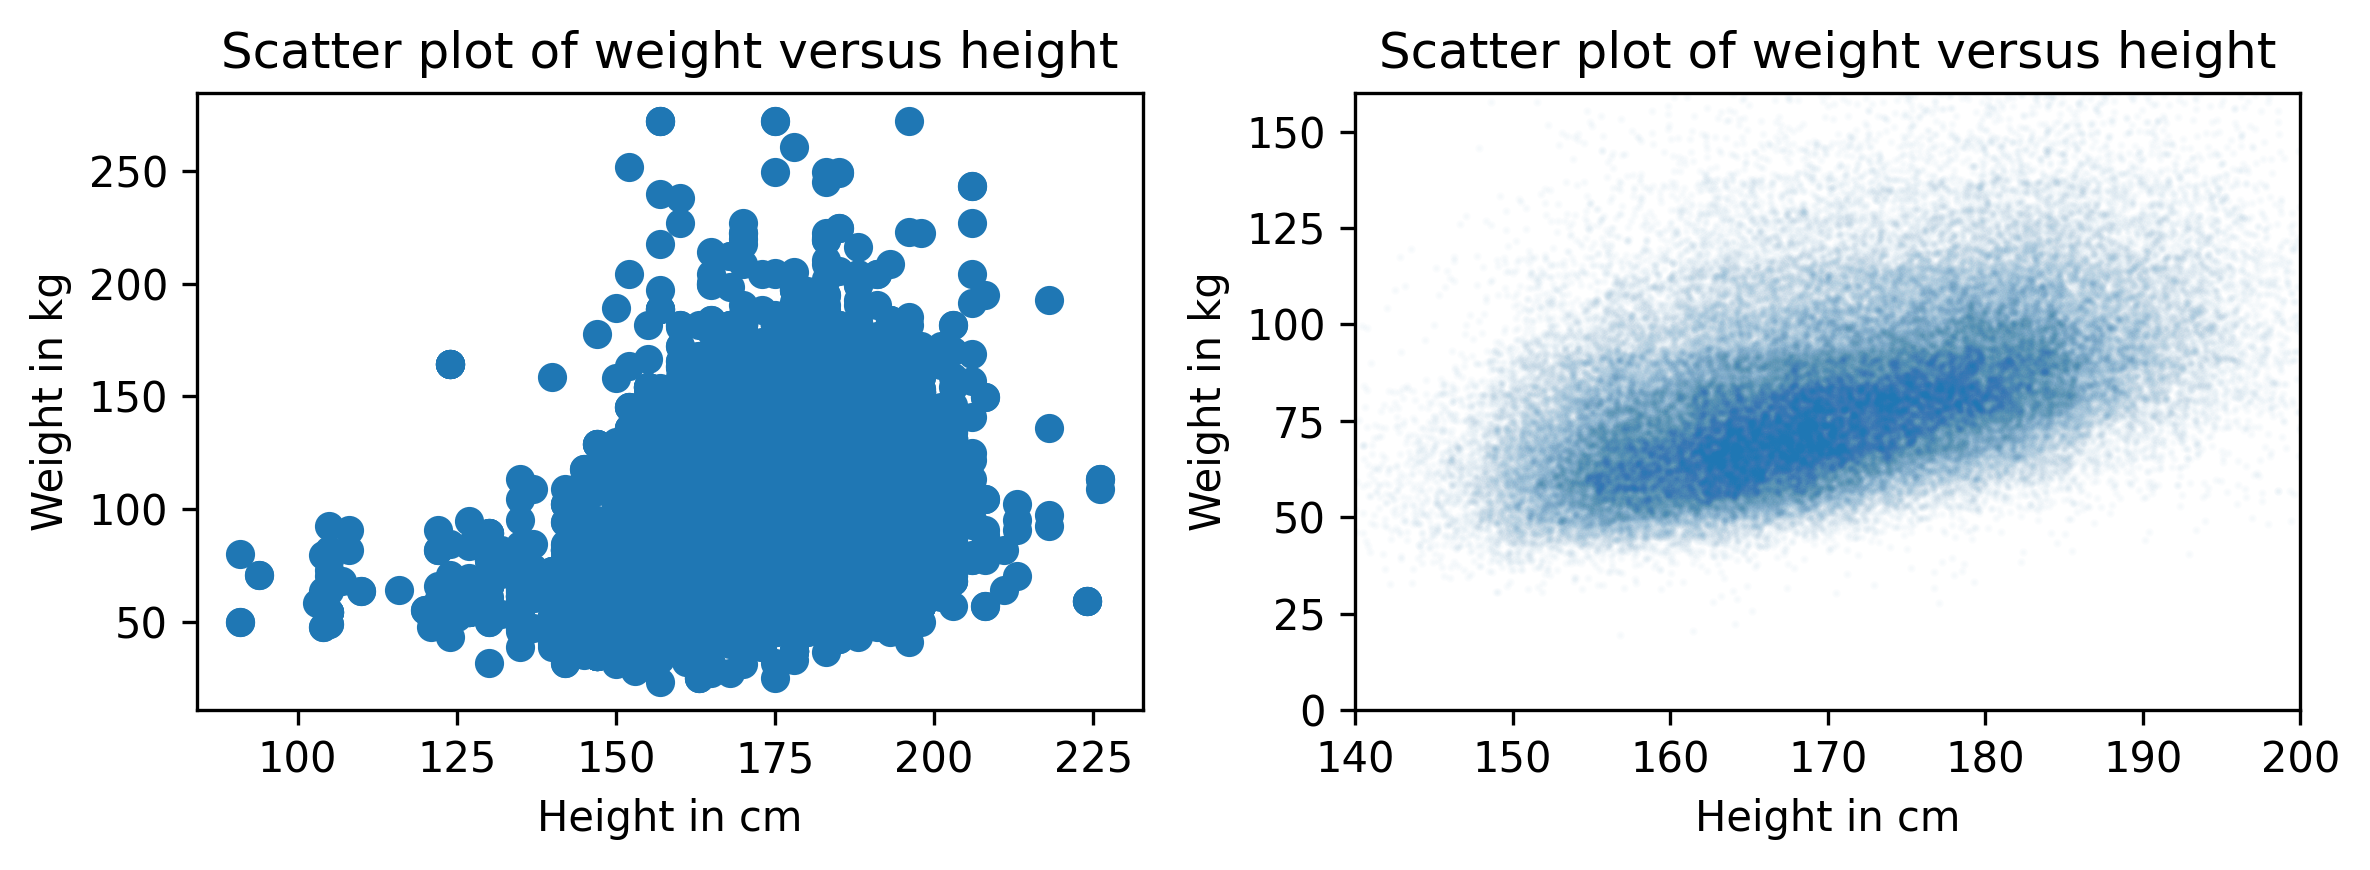
\includegraphics[width=4in]{chapters/09_relationships_files/09_relationships_27_0.png}
\end{center}

The point of this example is that it takes some effort to make an
effective scatter plot.

\textbf{Exercise:} Do people tend to gain weight as they get older? We
can answer this question by visualizing the relationship between weight
and age.

But before we make a scatter plot, it is a good idea to visualize
distributions one variable at a time. So let's look at the distribution
of age.

The BRFSS dataset includes a column, \passthrough{\lstinline!AGE!},
which represents each respondent's age in years. To protect respondents'
privacy, ages are rounded off into 5-year bins.
\passthrough{\lstinline!AGE!} contains the midpoint of the bins.

\begin{itemize}
\item
  Extract the variable \passthrough{\lstinline!'AGE'!} from the
  DataFrame \passthrough{\lstinline!brfss!} and assign it to
  \passthrough{\lstinline!age!}.
\item
  Plot the PMF of \passthrough{\lstinline!age!} as a bar chart, using
  \passthrough{\lstinline!Pmf!} from
  \passthrough{\lstinline!empiricaldist!}.
\end{itemize}

\begin{lstlisting}[]
from empiricaldist import Pmf
\end{lstlisting}

\textbf{Exercise:} Now let's look at the distribution of weight. The
column that contains weight in kilograms is
\passthrough{\lstinline!WTKG3!}. Because this column contains many
unique values, displaying it as a PMF doesn't work very well.

\begin{lstlisting}[]
Pmf.from_seq(weight).bar()

plt.xlabel('Weight in kg')
plt.ylabel('PMF')
plt.title('Distribution of weight');
\end{lstlisting}

\begin{center}
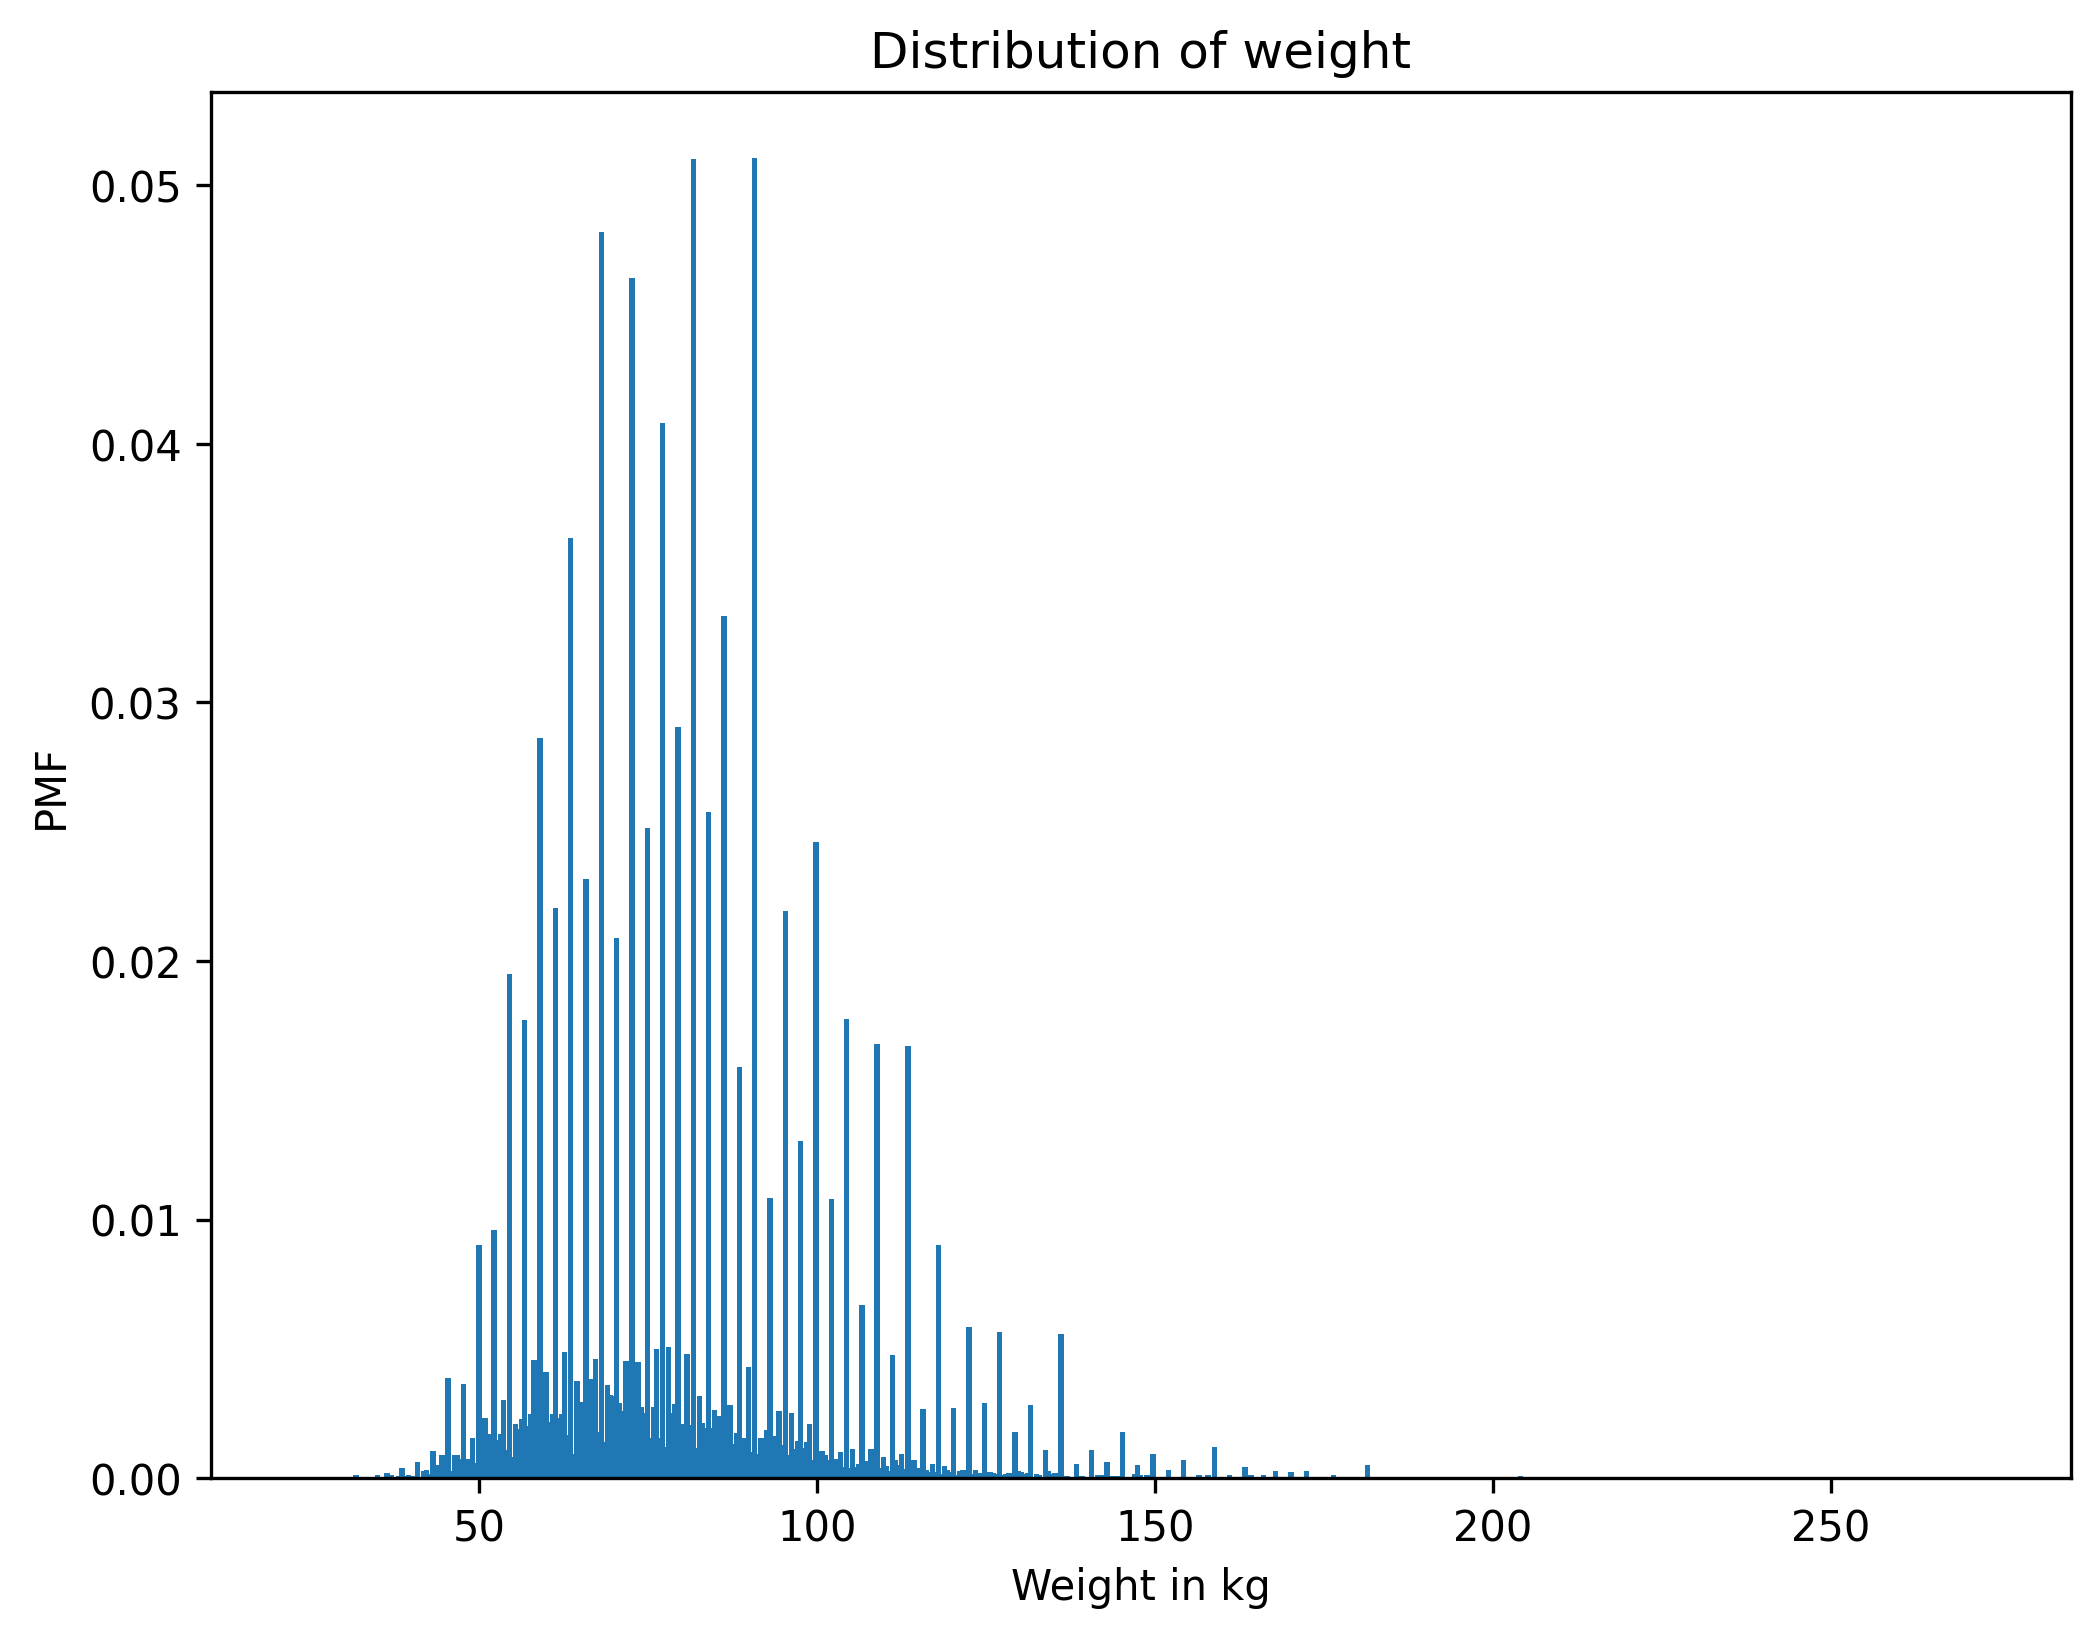
\includegraphics[width=4in]{chapters/09_relationships_files/09_relationships_33_0.png}
\end{center}

To get a better view of this distribution, try plotting the CDF.

Compute the CDF of a normal distribution with the same mean and standard
deviation, and compare it with the distribution of weight. Is the normal
distribution a good model for this data? What about log-transformed
weights?

\textbf{Exercise:} Now let's make a scatter plot of
\passthrough{\lstinline!weight!} versus \passthrough{\lstinline!age!}.
Adjust \passthrough{\lstinline!alpha!} and
\passthrough{\lstinline!markersize!} to avoid overplotting. Use
\passthrough{\lstinline!ylim!} to limit the \passthrough{\lstinline!y!}
axis from 0 to 200 kilograms.

\textbf{Exercise:} In the previous exercise, the ages fall in columns
because they've been rounded into 5-year bins. If we jitter them, the
scatter plot will show the relationship more clearly.

\begin{itemize}

\item
  Add random noise to \passthrough{\lstinline!age!} with mean
  \passthrough{\lstinline!0!} and standard deviation
  \passthrough{\lstinline!2.5!}.
\item
  Make a scatter plot and adjust \passthrough{\lstinline!alpha!} and
  \passthrough{\lstinline!markersize!} again.
\end{itemize}

\hypertarget{visualizing-relationships}{%
\section{Visualizing relationships}\label{visualizing-relationships}}

In the previous section we used scatter plots to visualize relationships
between variables, and in the exercises, you explored the relationship
between age and weight. In this section, we'll see other ways to
visualize these relationships, including boxplots and violin plots.

Let's start with a scatter plot of weight versus age.

\begin{lstlisting}[]
age = brfss['AGE']
noise = np.random.normal(0, 1.0, size=len(brfss))
age_jitter = age + noise

plt.plot(age_jitter, weight_jitter, 'o', 
         alpha=0.01, markersize=1)

plt.xlabel('Age in years')
plt.ylabel('Weight in kg')
plt.ylim([0, 200])
plt.title('Weight versus age');
\end{lstlisting}

\begin{center}
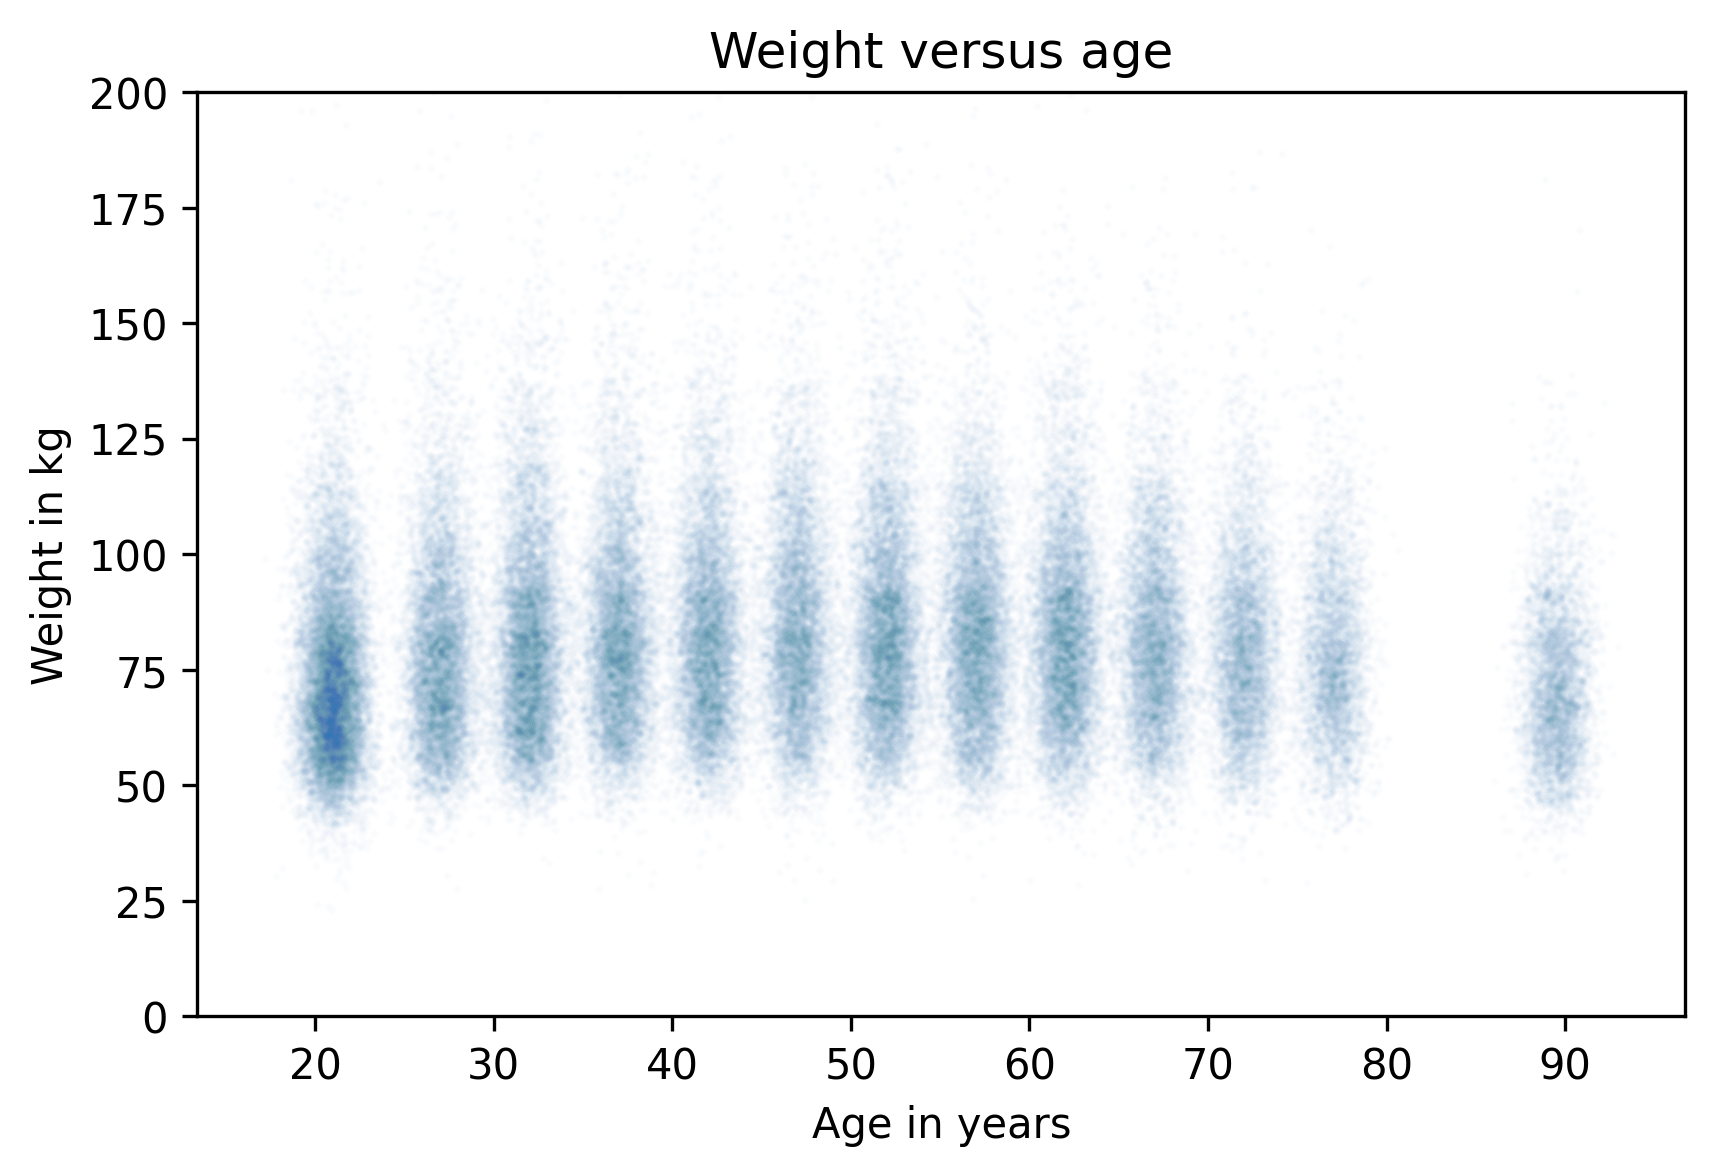
\includegraphics[width=4in]{chapters/09_relationships_files/09_relationships_38_0.png}
\end{center}

In this version of the scatter plot, the weights are jittered, but
there's still space between the columns. That makes it possible to see
the shape of the distribution in each age group, and the differences
between groups. With this view, it looks like weight increases until age
40 or 50, and then starts to decrease.

If we take this idea one step farther, we can use KDE to estimate the
density function in each column and plot it. And there's a name for
that; it's called a \textbf{violin plot}. Seaborn provides a function
that makes violin plots, but before we can use it, we have to get rid of
any rows with missing data. Here's how:

\begin{lstlisting}[]
data = brfss.dropna(subset=['AGE', 'WTKG3'])
data.shape
(@\dashfill@)
@@@(92729, 9)@@@
\end{lstlisting}

\passthrough{\lstinline!dropna()!} creates a new DataFrame that drops
the rows in \passthrough{\lstinline!brfss!} where
\passthrough{\lstinline!AGE!} or \passthrough{\lstinline!WTKG3!} are
\passthrough{\lstinline!NaN!}. Now we can call
\passthrough{\lstinline!violinplot!}.

\begin{lstlisting}[]
import seaborn as sns

sns.violinplot(x='AGE', y='WTKG3', data=data, inner=None)

plt.xlabel('Age in years')
plt.ylabel('Weight in kg')
plt.title('Weight versus age');
\end{lstlisting}

\begin{center}
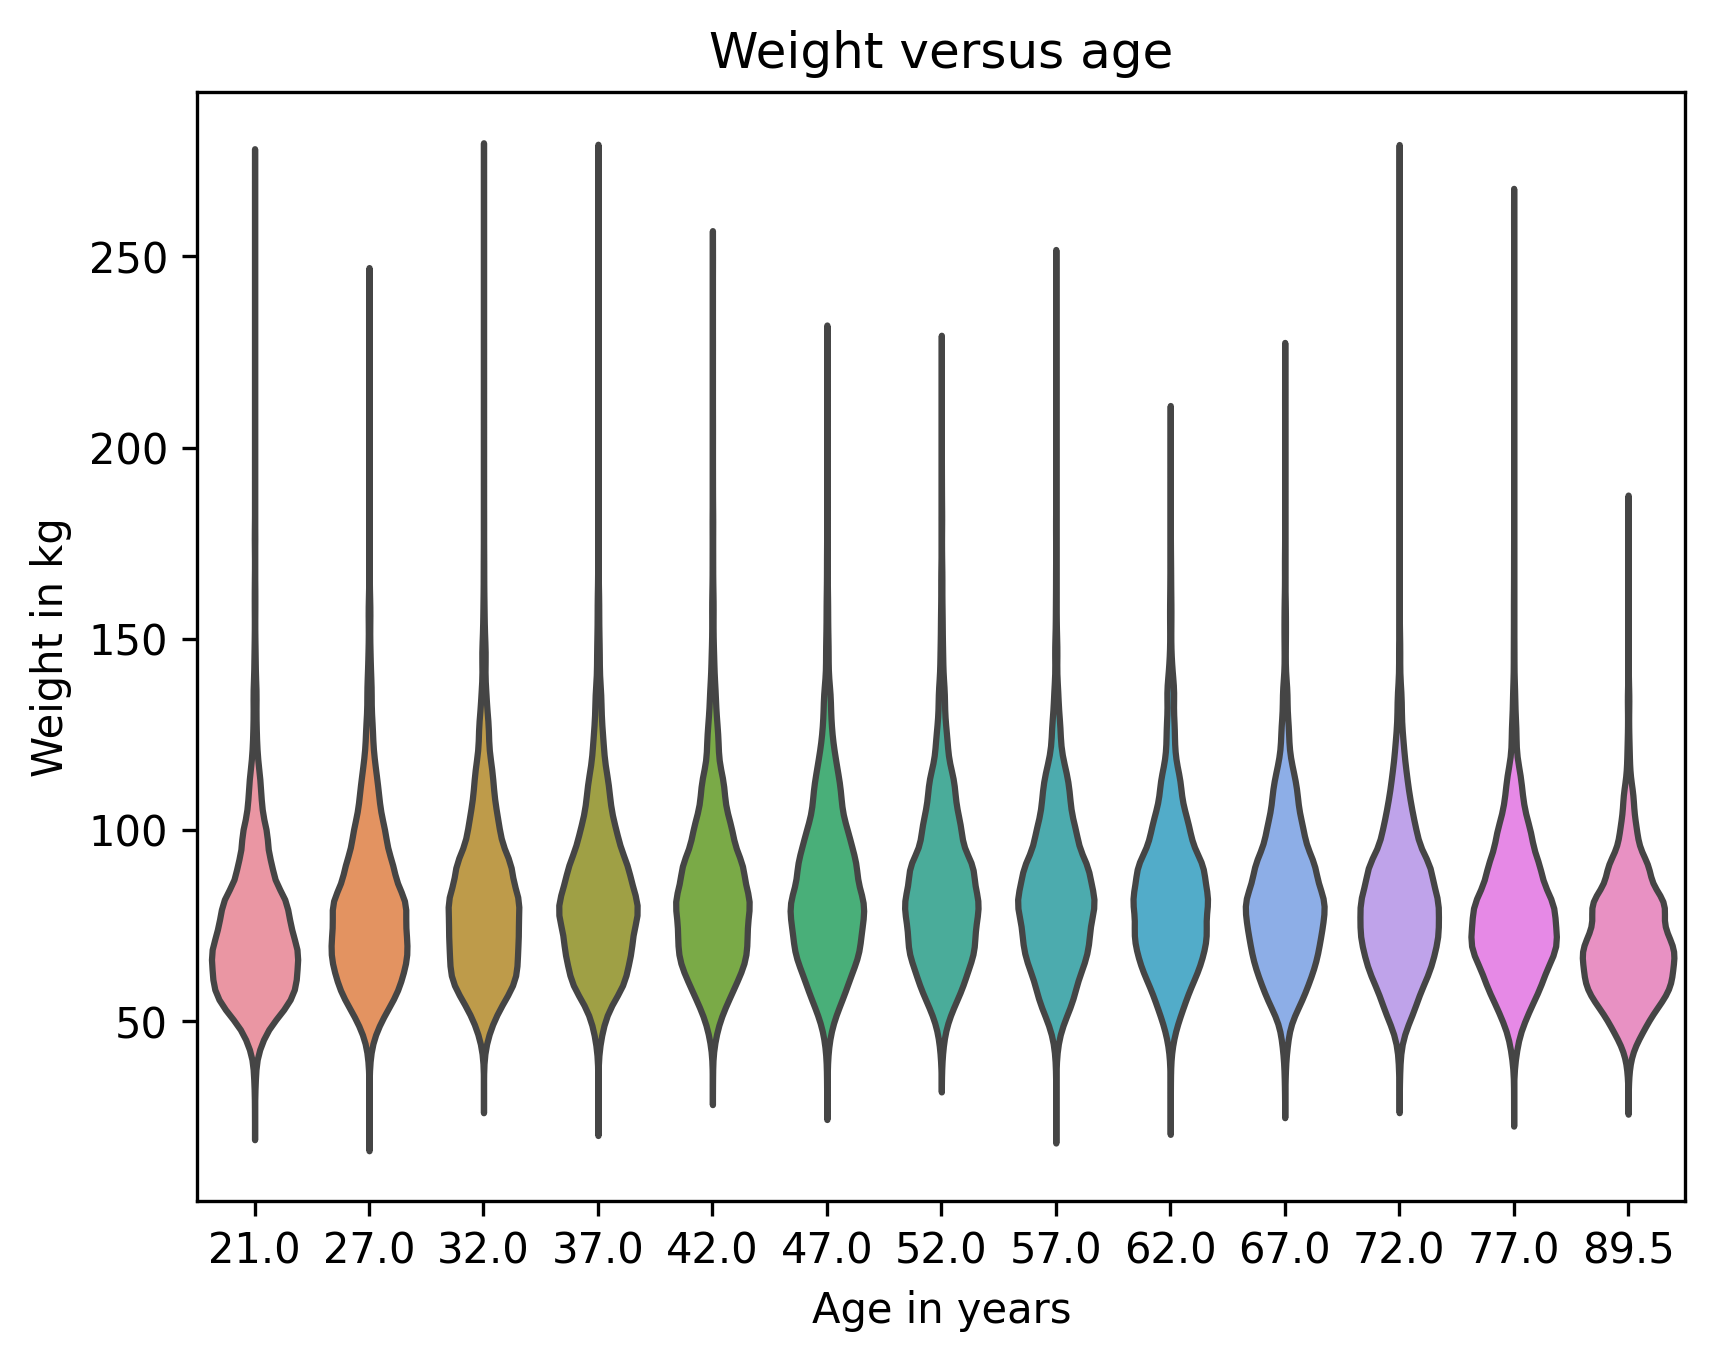
\includegraphics[width=4in]{chapters/09_relationships_files/09_relationships_42_0.png}
\end{center}

The \passthrough{\lstinline!x!} and \passthrough{\lstinline!y!}
arguments mean we want \passthrough{\lstinline!AGE!} on the x-axis and
\passthrough{\lstinline!WTKG3!} on the y-axis.
\passthrough{\lstinline!data!} is the DataFrame we just created, which
contains the variables we're going to plot. The argument
\passthrough{\lstinline!inner=None!} simplifies the plot a little.

In the figure, each shape represents the distribution of weight in one
age group. The width of these shapes is proportional to the estimated
density, so it's like two vertical KDEs plotted back to back.

Another, related way to look at data like this is called a \textbf{box
plot}, which represents summary statistics for the values in each
group.\\
The code to generate a box plot is very similar.

\begin{lstlisting}[]
sns.boxplot(x='AGE', y='WTKG3', data=data, whis=10)

plt.xlabel('Age in years')
plt.ylabel('Weight in kg')
plt.title('Weight versus age');
\end{lstlisting}

\begin{center}
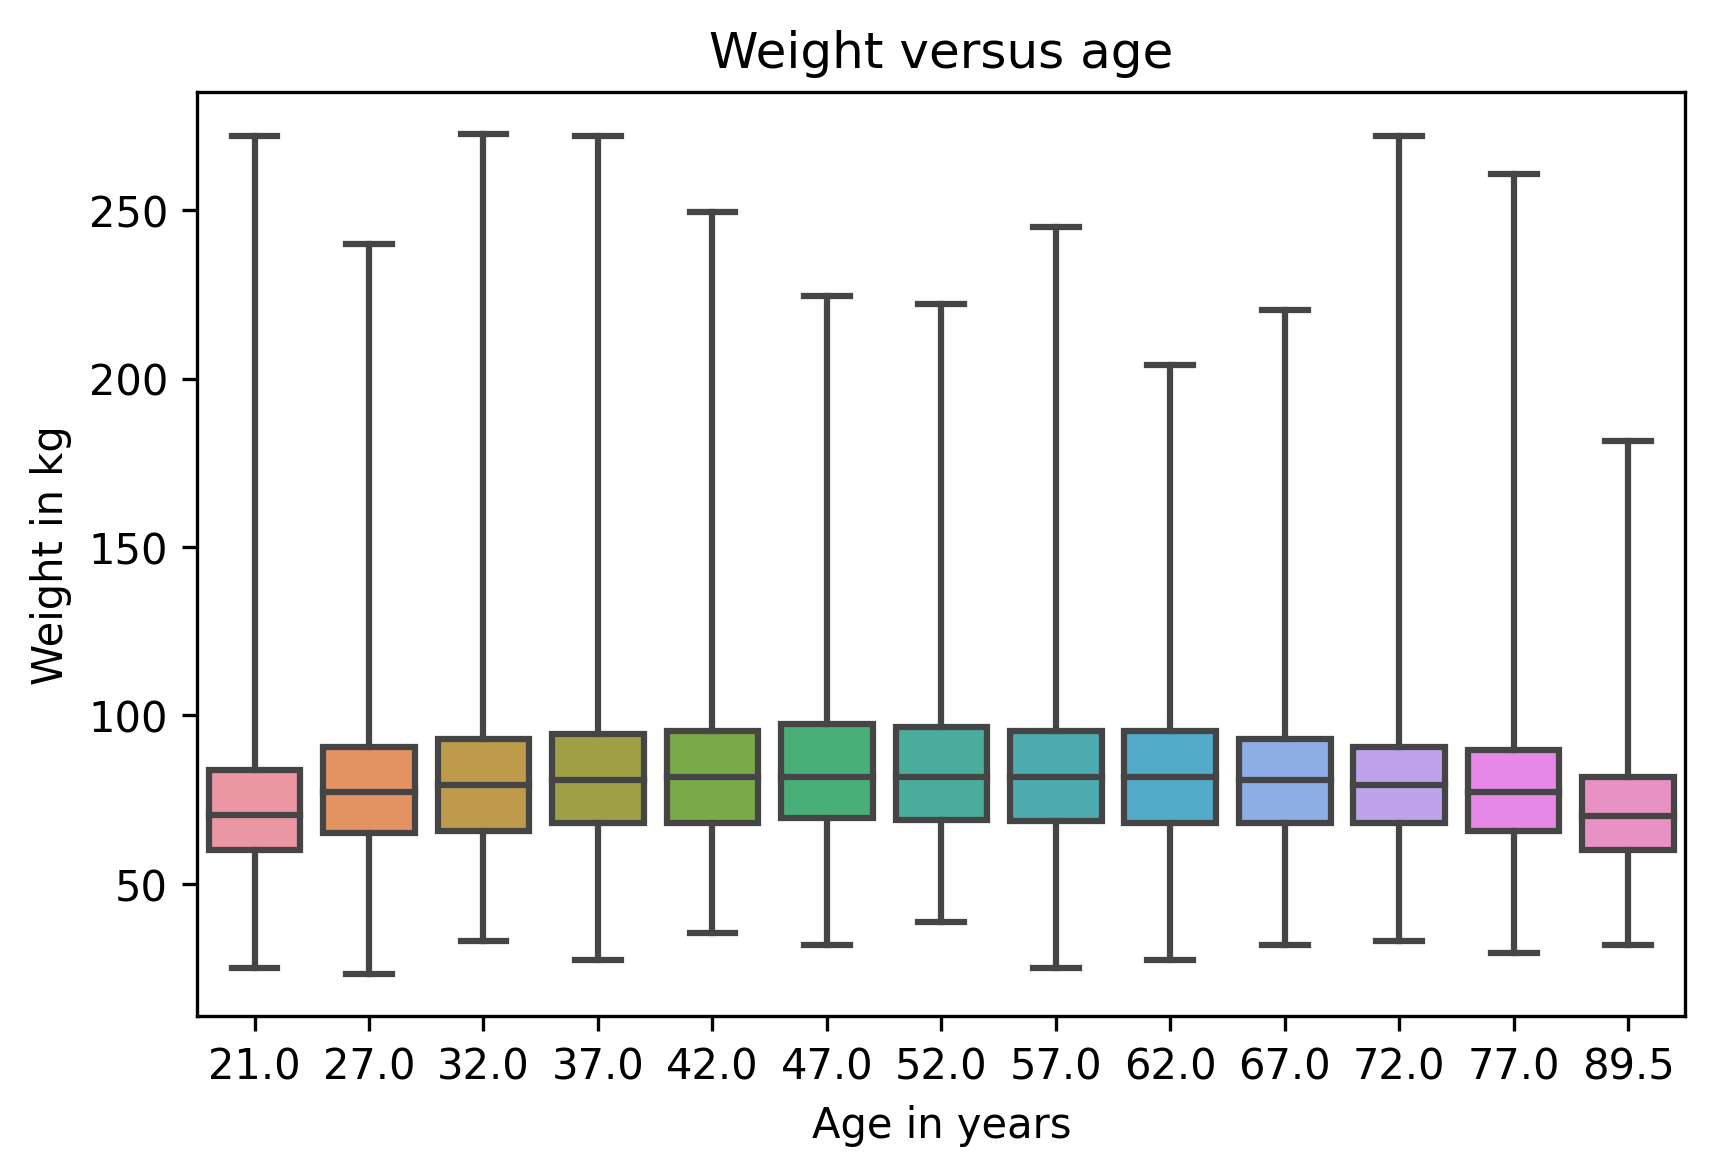
\includegraphics[width=4in]{chapters/09_relationships_files/09_relationships_44_0.png}
\end{center}

The argument \passthrough{\lstinline!whis=10!} turns off a feature we
don't need. If you are curious about it, you can
\href{https://seaborn.pydata.org/generated/seaborn.boxplot.html}{read
the documentation}.

Each box represents the distribution of weight in an age group. The
height of each box represents the range from the 25th to the 75th
percentile. The line in the middle of each box is the median. The spines
sticking out of the top and bottom show the minimum and maximum values.

In my opinion, this plot gives us the best view of the relationship
between weight and age.

\begin{itemize}
\item
  Looking at the medians, it seems like people in their 40s are the
  heaviest; younger and older people are lighter.
\item
  Looking at the sizes of the boxes, it seems like people in their 40s
  have the most variability in weight, too.
\item
  These plots also show how skewed the distribution of weight is; that
  is, the heaviest people are much farther from the median than the
  lightest people.
\end{itemize}

For data that skews toward higher values, it is sometimes useful to look
at it on a logarithmic scale. We can do that with the Pyplot function
\passthrough{\lstinline!yscale!}.

\begin{lstlisting}[]
sns.boxplot(x='AGE', y='WTKG3', data=data, whis=10)

plt.yscale('log')
plt.xlabel('Age in years')
plt.ylabel('Weight in kg (log scale)')
plt.title('Weight versus age');
\end{lstlisting}

\begin{center}
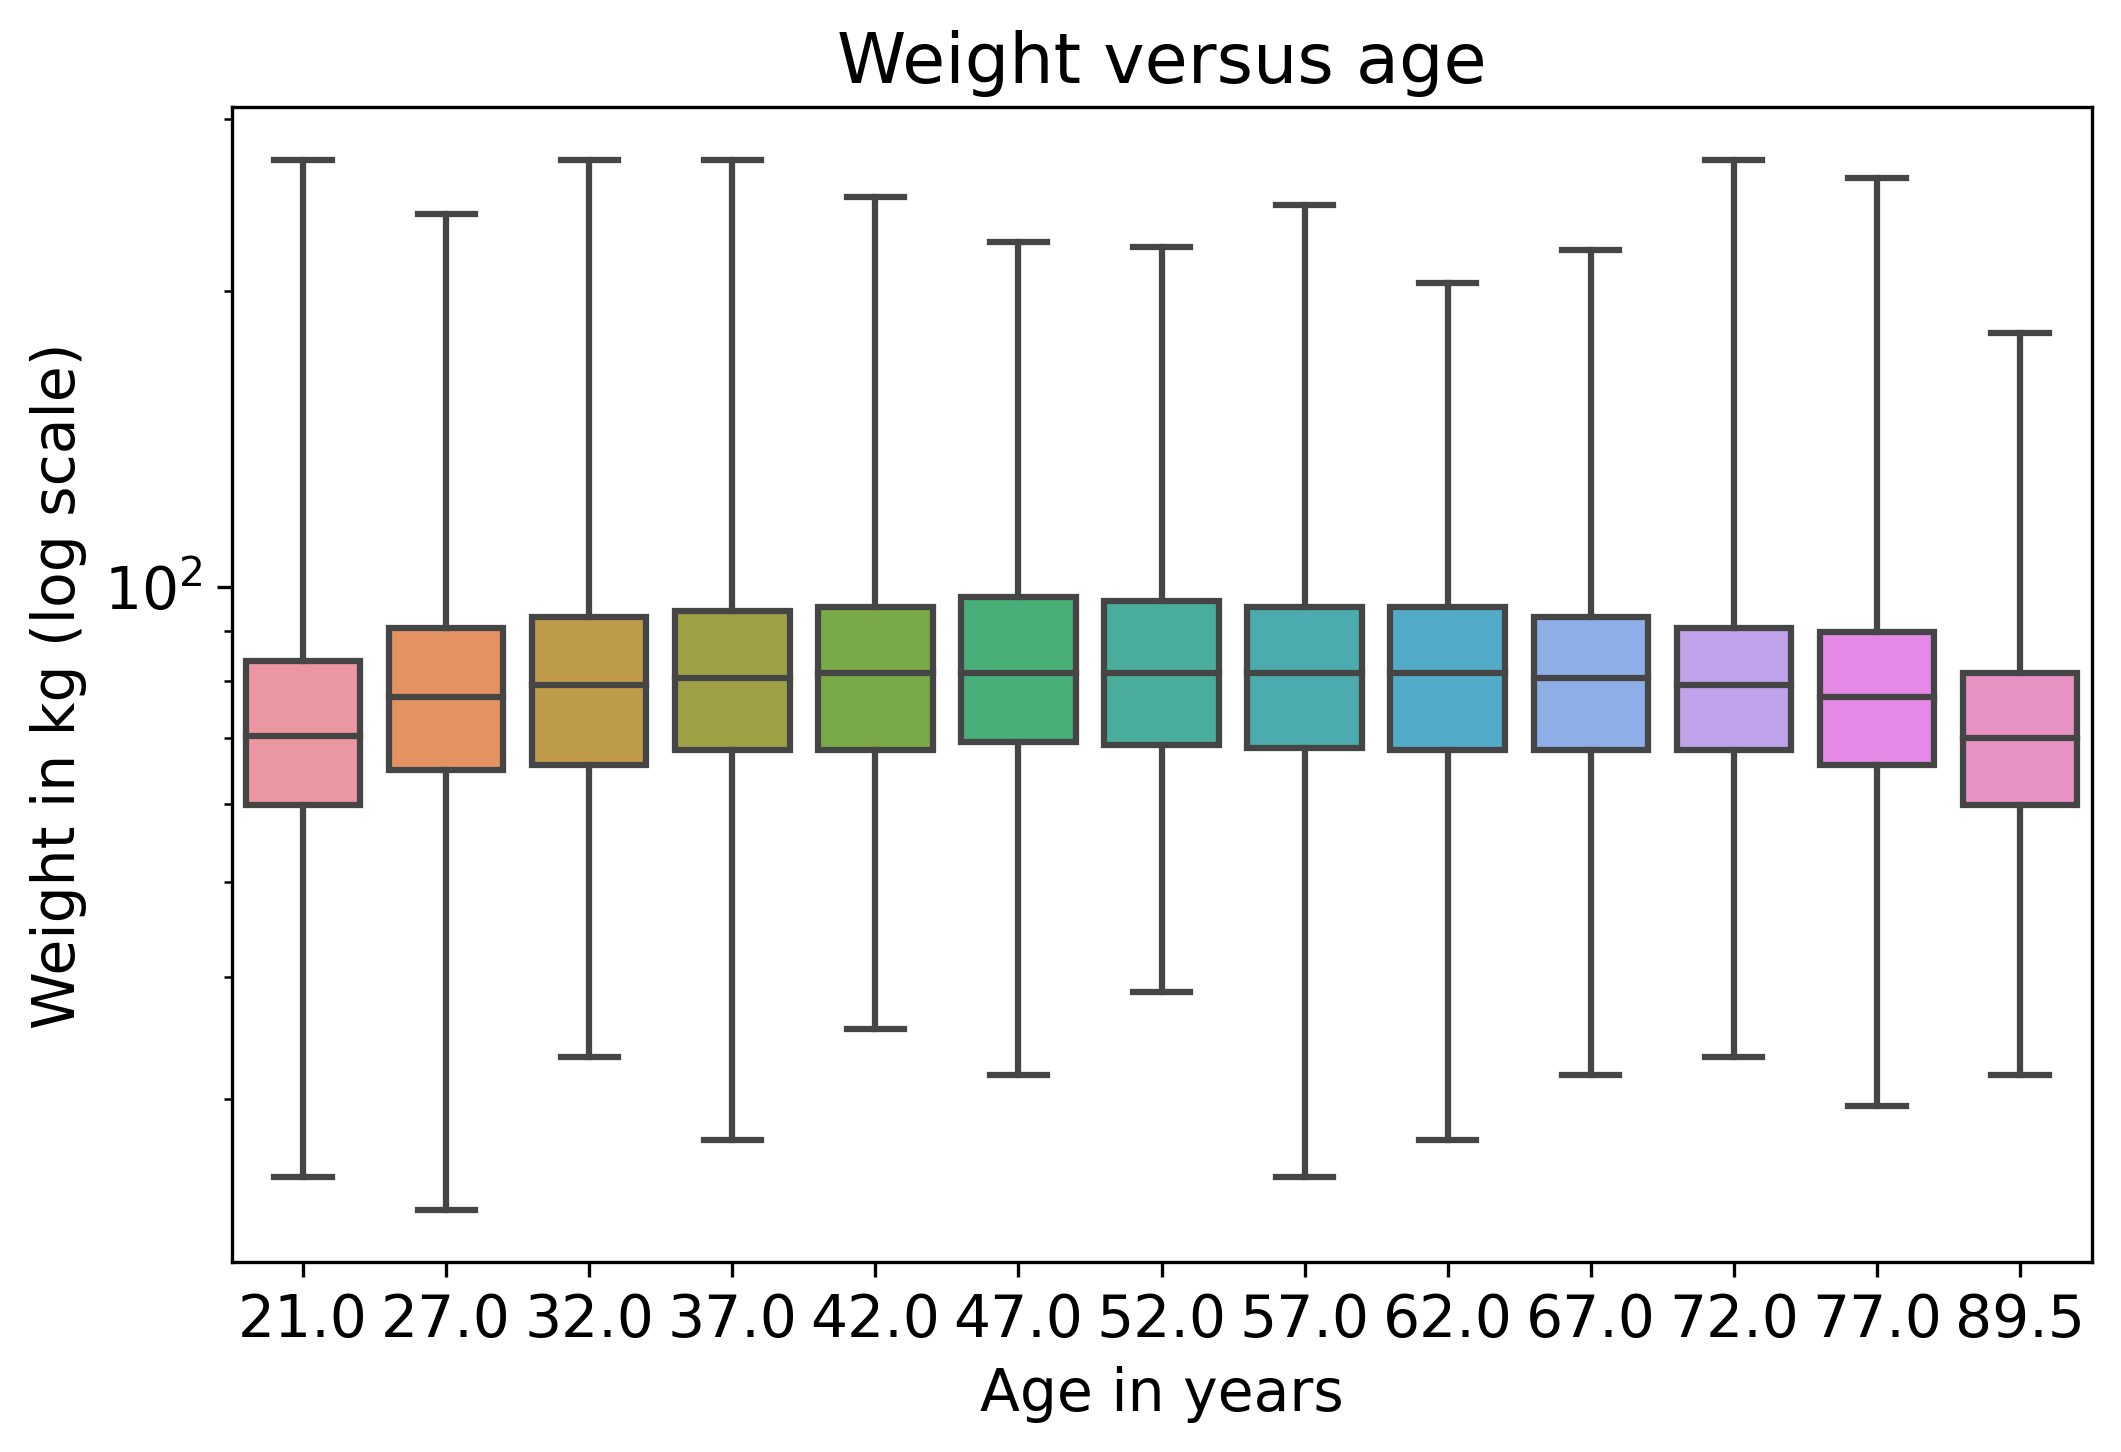
\includegraphics[width=4in]{chapters/09_relationships_files/09_relationships_46_0.png}
\end{center}

On a log scale, the distributions are symmetric, so the spines are the
same length, the boxes are close to the middle of the figure, and we can
see the relationship between age and weight more clearly.

In the following exercises, you'll have a chance to generate violin and
box plots for other variables.

\textbf{Exercise:} Previously we looked at a scatter plot of height and
weight, and saw that taller people tend to be heavier. Now let's take a
closer look using a box plot. The \passthrough{\lstinline!brfss!}
DataFrame contains a column named \passthrough{\lstinline!\_HTMG10!}
that represents height in centimeters, binned into 10 cm groups.

\begin{itemize}
\item
  Make a boxplot that shows the distribution of weight in each height
  group.
\item
  Plot the y-axis on a logarithmic scale.
\end{itemize}

Suggestion: If the labels on the \passthrough{\lstinline!x!} axis
collide, you can rotate them like this:

\begin{lstlisting}
plt.xticks(rotation='45')
\end{lstlisting}

\textbf{Exercise:} As a second example, let's look at the relationship
between income and height.

In the BRFSS, income is represented as a categorical variable; that is,
respondents are assigned to one of 8 income categories. The column name
is \passthrough{\lstinline!INCOME2!}.

Before we connect income with anything else, let's look at the
distribution by computing the PMF.

\begin{itemize}
\item
  Extract \passthrough{\lstinline!INCOME2!} from
  \passthrough{\lstinline!brfss!} and assign it to
  \passthrough{\lstinline!income!}.
\item
  Plot the PMF of \passthrough{\lstinline!income!} as a bar chart.
\end{itemize}

Note: You will see that about a third of the respondents are in the
highest income group; ideally, it would be better if there were more
groups at the high end, but we'll work with what we have.

\textbf{Exercise:} Generate a violin plot that shows the distribution of
height in each income group. Can you see a relationship between these
variables?

\hypertarget{quantifying-correlation}{%
\section{Quantifying Correlation}\label{quantifying-correlation}}

In the previous section, we visualized relationships between pairs of
variables. Now we'll learn about the \textbf{coefficient of
correlation}, which quantifies the strength of these relationships.

When people say ``correlation'' casually, they might mean any
relationship between two variables. In statistics, it usually means
Pearson's correlation coefficient, which is a number between
\passthrough{\lstinline!-1!} and \passthrough{\lstinline!1!} that
quantifies the strength of a linear relationship between variables.

To demonstrate, we'll select three columns from the BRFSS dataset:

\begin{lstlisting}[]
columns = ['HTM4', 'WTKG3', 'AGE']
subset = brfss[columns]
\end{lstlisting}

The result is a DataFrame with just those columns. With this subset of
the data, we can use the \passthrough{\lstinline!corr!} method, like
this:

\begin{lstlisting}[]
subset.corr()
(@\dashfill@)
@@@/home/downey/miniconda3/envs/ElementsOfDataScience/lib/python3.8/site-packages/IPython/core/formatters.py:342: FutureWarning: In future versions `DataFrame.to_latex` is expected to utilise the base implementation of `Styler.to_latex` for formatting and rendering. The arguments signature may therefore change. It is recommended instead to use `DataFrame.style.to_latex` which also contains additional functionality.
  return method()@@@
\end{lstlisting}

\begin{tabular}{lrrr}
\midrule
{} &      HTM4 &     WTKG3 &       AGE \\
\midrule
HTM4  &  1.000000 &  0.474203 & -0.093684 \\
WTKG3 &  0.474203 &  1.000000 &  0.021641 \\
AGE   & -0.093684 &  0.021641 &  1.000000 \\
\midrule
\end{tabular}

The result is a \textbf{correlation matrix}. Reading across the first
row, the correlation of \passthrough{\lstinline!HTM4!} with itself is
\passthrough{\lstinline!1!}. That's expected; the correlation of
anything with itself is \passthrough{\lstinline!1!}.

The next entry is more interesting; the correlation of height and weight
is about \passthrough{\lstinline!0.47!}. It's positive, which means
taller people are heavier, and it is moderate in strength, which means
it has some predictive value, but not much. If you know someone's
height, you can make a somewhat better guess about their weight.

The correlation between height and age is about
\passthrough{\lstinline!-0.09!}. It's negative, which means that older
people tend to be shorter, but it's weak, which means that knowing
someone's age would not help much if you were trying to guess their
height.

The correlation between age and weight is even smaller. It is tempting
to conclude that there is no relationship between age and weight, but we
have already seen that there is. So why is the correlation so low?
Remember that the relationship between weight and age looks like this.

\begin{lstlisting}[]
data = brfss.dropna(subset=['AGE', 'WTKG3'])
sns.boxplot(x='AGE', y='WTKG3', data=data, whis=10)

plt.xlabel('Age in years')
plt.ylabel('Weight in kg')
plt.title('Weight versus age');
\end{lstlisting}

\begin{center}
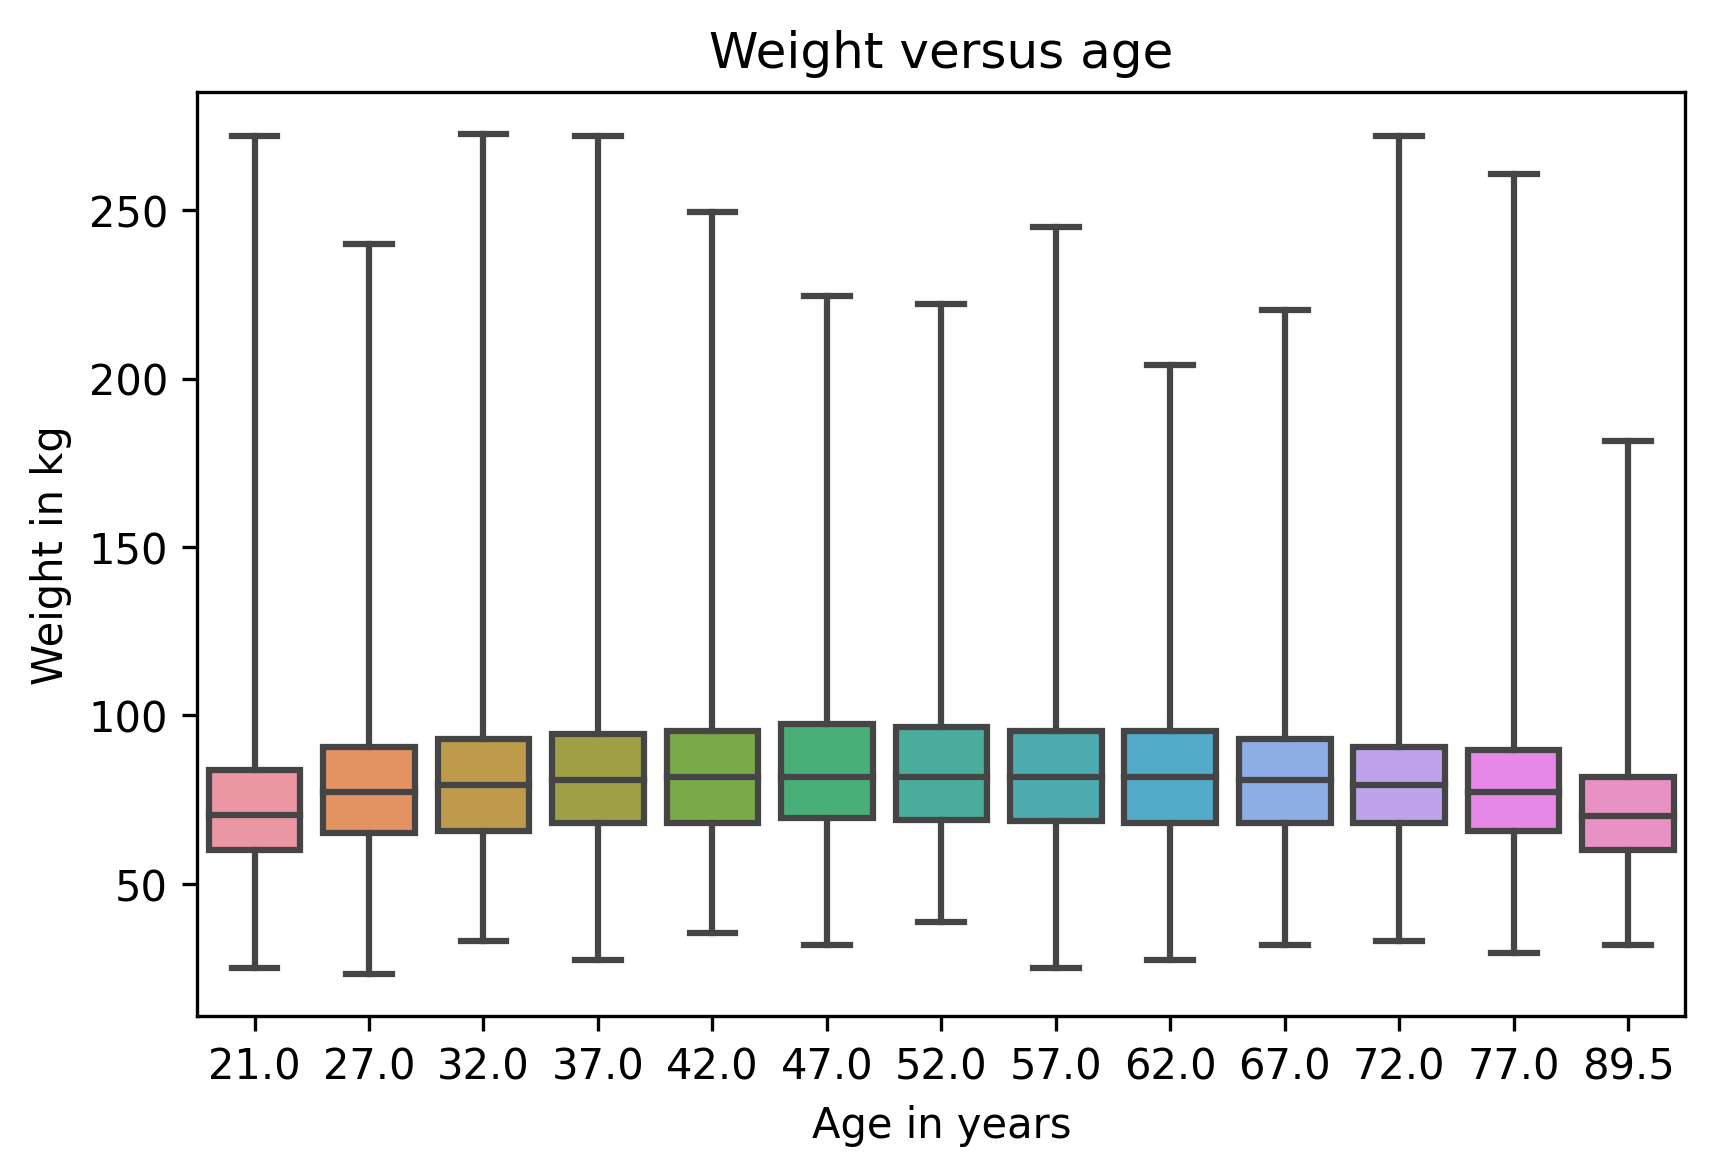
\includegraphics[width=4in]{chapters/09_relationships_files/09_relationships_57_0.png}
\end{center}

People in their forties are the heaviest; younger and older people are
lighter. So this relationship is nonlinear. But correlation only
measures linear relationships. If the relationship is nonlinear,
correlation generally underestimates how strong it is.

To demonstrate, I'll generate some fake data:
\passthrough{\lstinline!xs!} contains equally-spaced points between
\passthrough{\lstinline!-1!} and \passthrough{\lstinline!1!}.
\passthrough{\lstinline!ys!} is \passthrough{\lstinline!xs!} squared
plus some random noise.

\begin{lstlisting}[]
xs = np.linspace(-1, 1)
ys = xs**2 + np.random.normal(0, 0.05, len(xs))
\end{lstlisting}

Here's the scatter plot of \passthrough{\lstinline!xs!} and
\passthrough{\lstinline!ys!}.

\begin{lstlisting}[]
plt.plot(xs, ys, 'o', alpha=0.5)
plt.xlabel('x')
plt.ylabel('y')
plt.title('Scatter plot of a fake dataset');
\end{lstlisting}

\begin{center}
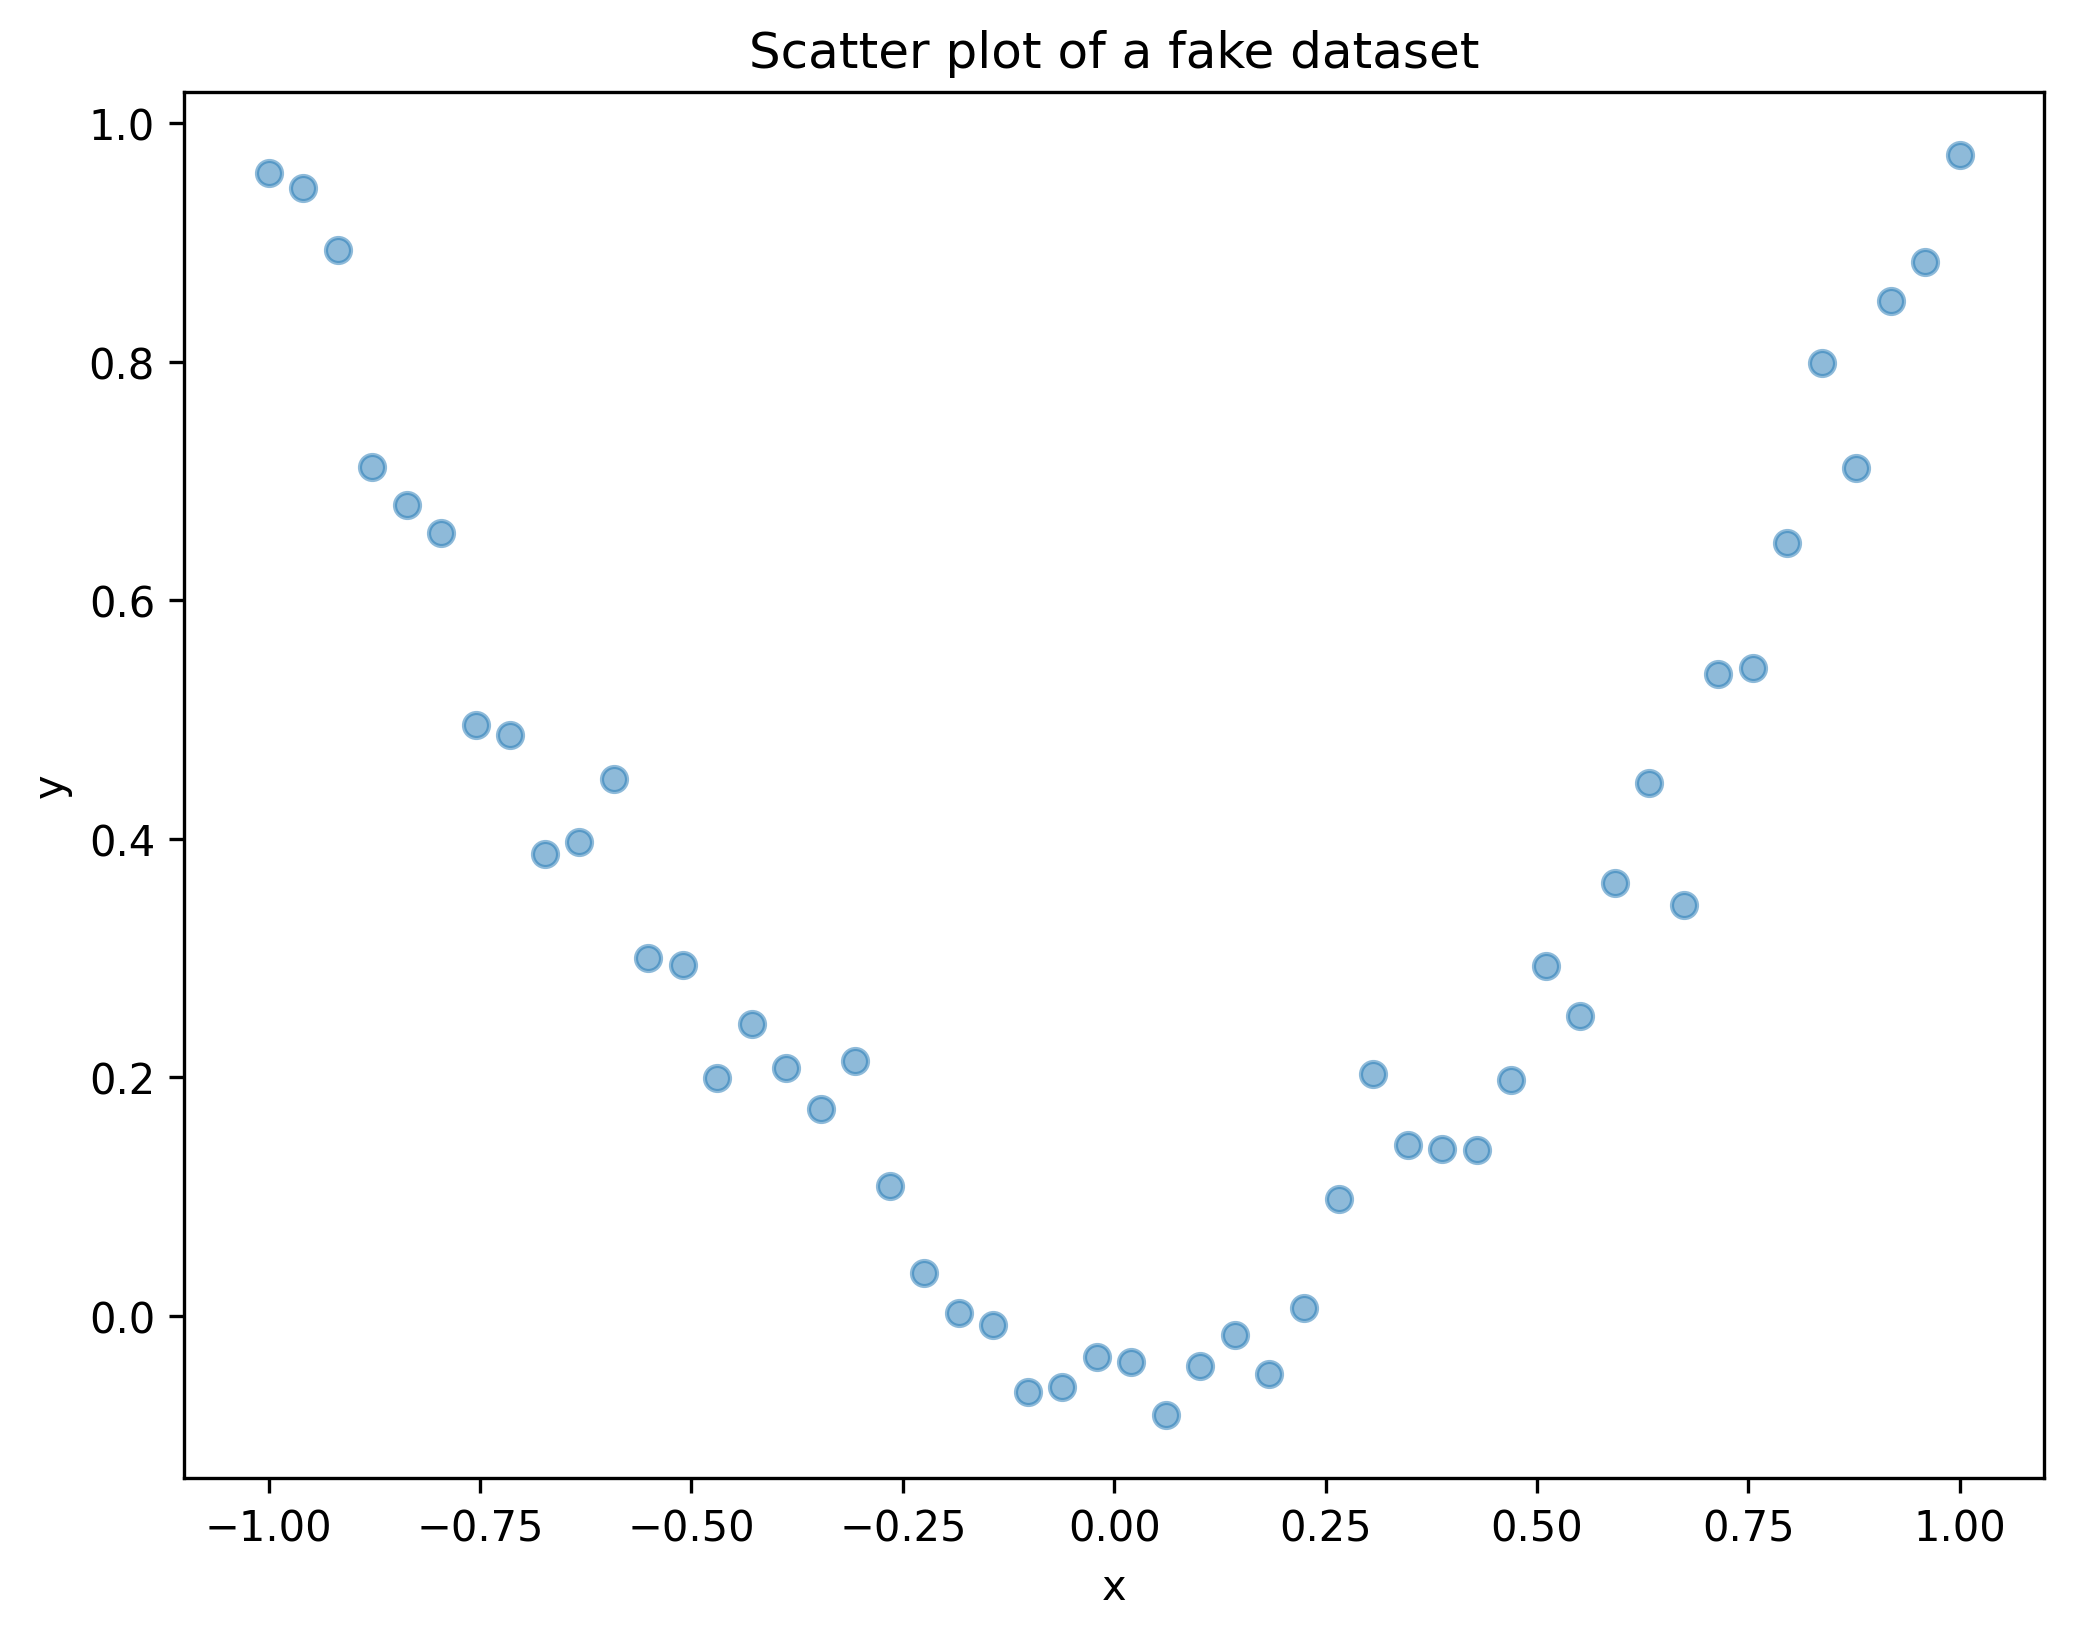
\includegraphics[width=4in]{chapters/09_relationships_files/09_relationships_61_0.png}
\end{center}

It's clear that this is a strong relationship; if you are given
\passthrough{\lstinline!x!}, you can make a much better guess about
\passthrough{\lstinline!y!}. But here's the correlation matrix:

\begin{lstlisting}[]
np.corrcoef(xs, ys)
(@\dashfill@)
@@@array([[1.        , 0.00856993],
       [0.00856993, 1.        ]])@@@
\end{lstlisting}

Even though there is a strong non-linear relationship, the computed
correlation is close to \passthrough{\lstinline!0!}.

In general, if correlation is high -- that is, close to
\passthrough{\lstinline!1!} or \passthrough{\lstinline!-1!} -- you can
conclude that there is a strong linear relationship. But if correlation
is close to \passthrough{\lstinline!0!}, that doesn't mean there is no
relationship; there might be a non-linear relationship.

This is one of the reasons I think correlation is not such a great
statistic. There's another reason to be careful with correlation; it
doesn't mean what people take it to mean. Specifically, correlation says
nothing about slope. If we say that two variables are correlated, that
means we can use one to predict the other. But that might not be what we
care about.

For example, suppose we are concerned about the health effects of weight
gain, so we plot weight versus age from 20 to 50 years old. I'll
generate two fake datasets to demonstrate the point. In each dataset,
\passthrough{\lstinline!xs!} represents age and
\passthrough{\lstinline!ys!} represents weight.

\begin{lstlisting}[]
np.random.seed(18)
xs1 = np.linspace(20, 50)
ys1 = 75 + 0.02 * xs1 + np.random.normal(0, 0.15, len(xs1))

plt.plot(xs1, ys1, 'o', alpha=0.5)
plt.xlabel('Age in years')
plt.ylabel('Weight in kg')
plt.title('Fake dataset #1');
\end{lstlisting}

\begin{center}
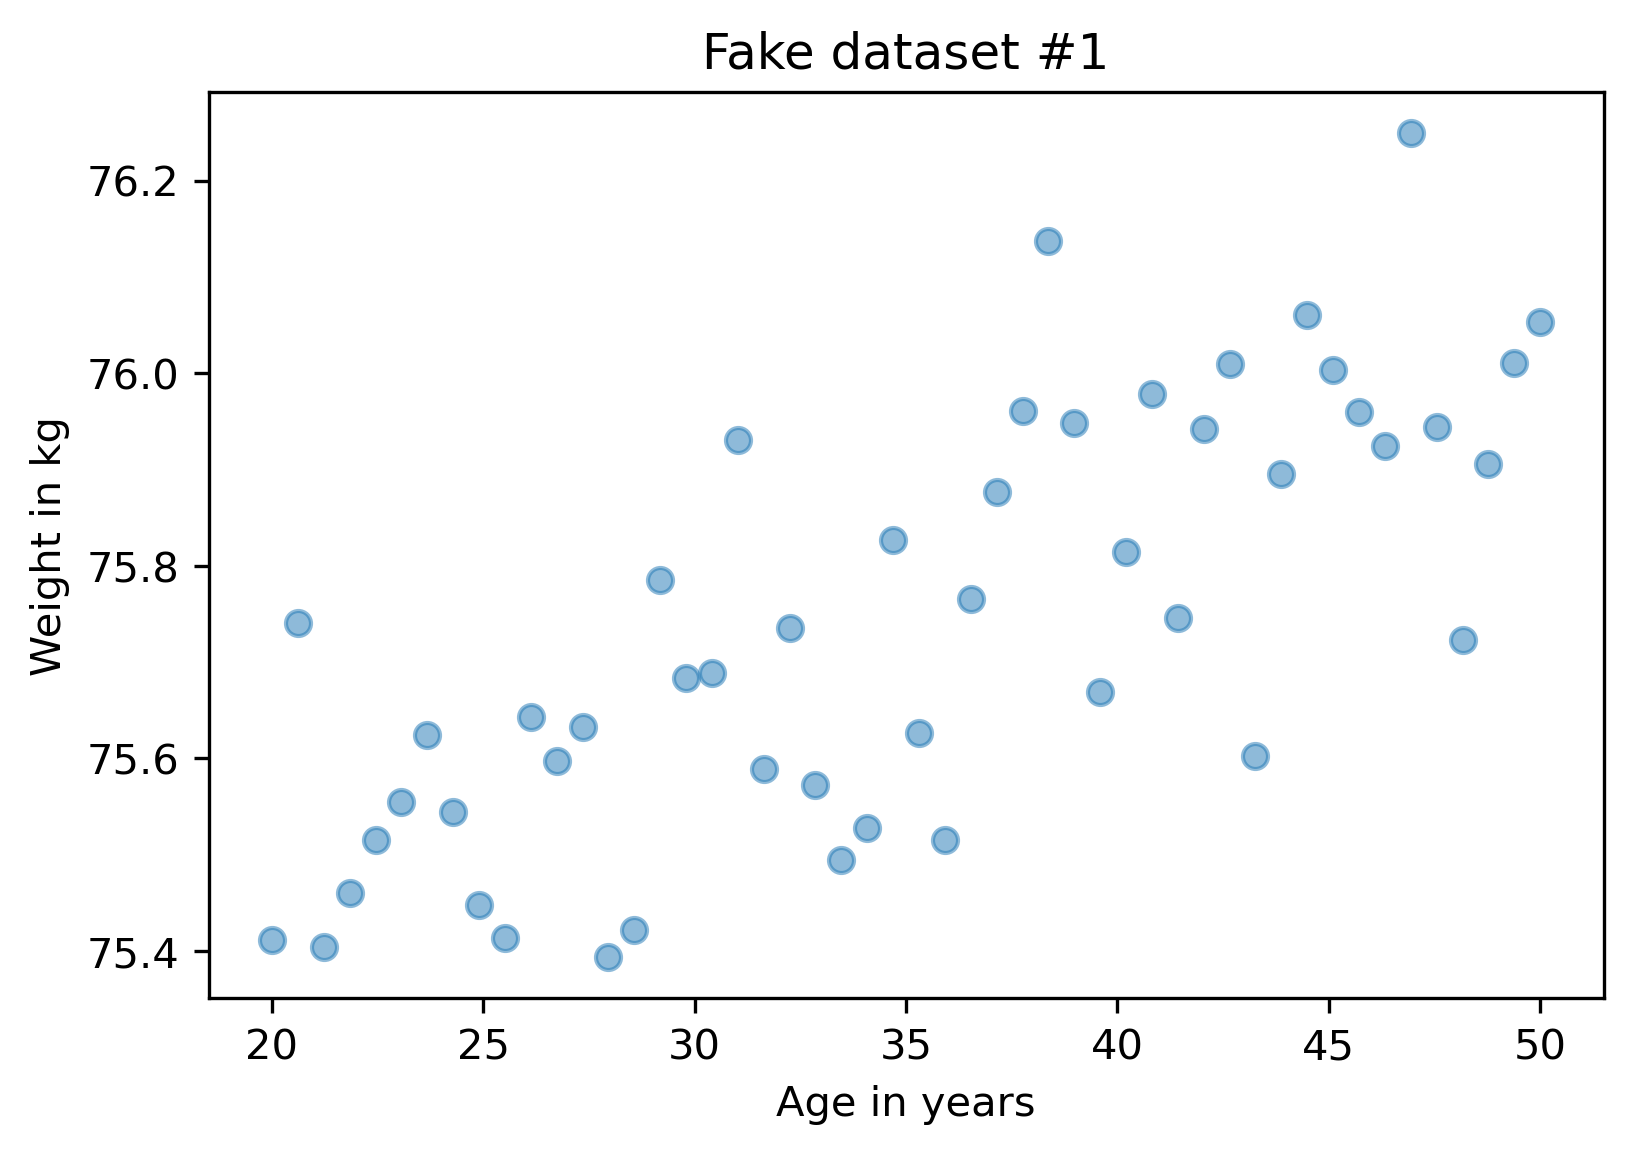
\includegraphics[width=4in]{chapters/09_relationships_files/09_relationships_66_0.png}
\end{center}

And here's the second dataset:

\begin{lstlisting}[]
np.random.seed(18)
xs2 = np.linspace(20, 50)
ys2 = 65 + 0.2 * xs2 + np.random.normal(0, 3, len(xs2))

plt.plot(xs2, ys2, 'o', alpha=0.5)
plt.xlabel('Age in years')
plt.ylabel('Weight in kg')
plt.title('Fake dataset #2');
\end{lstlisting}

\begin{center}
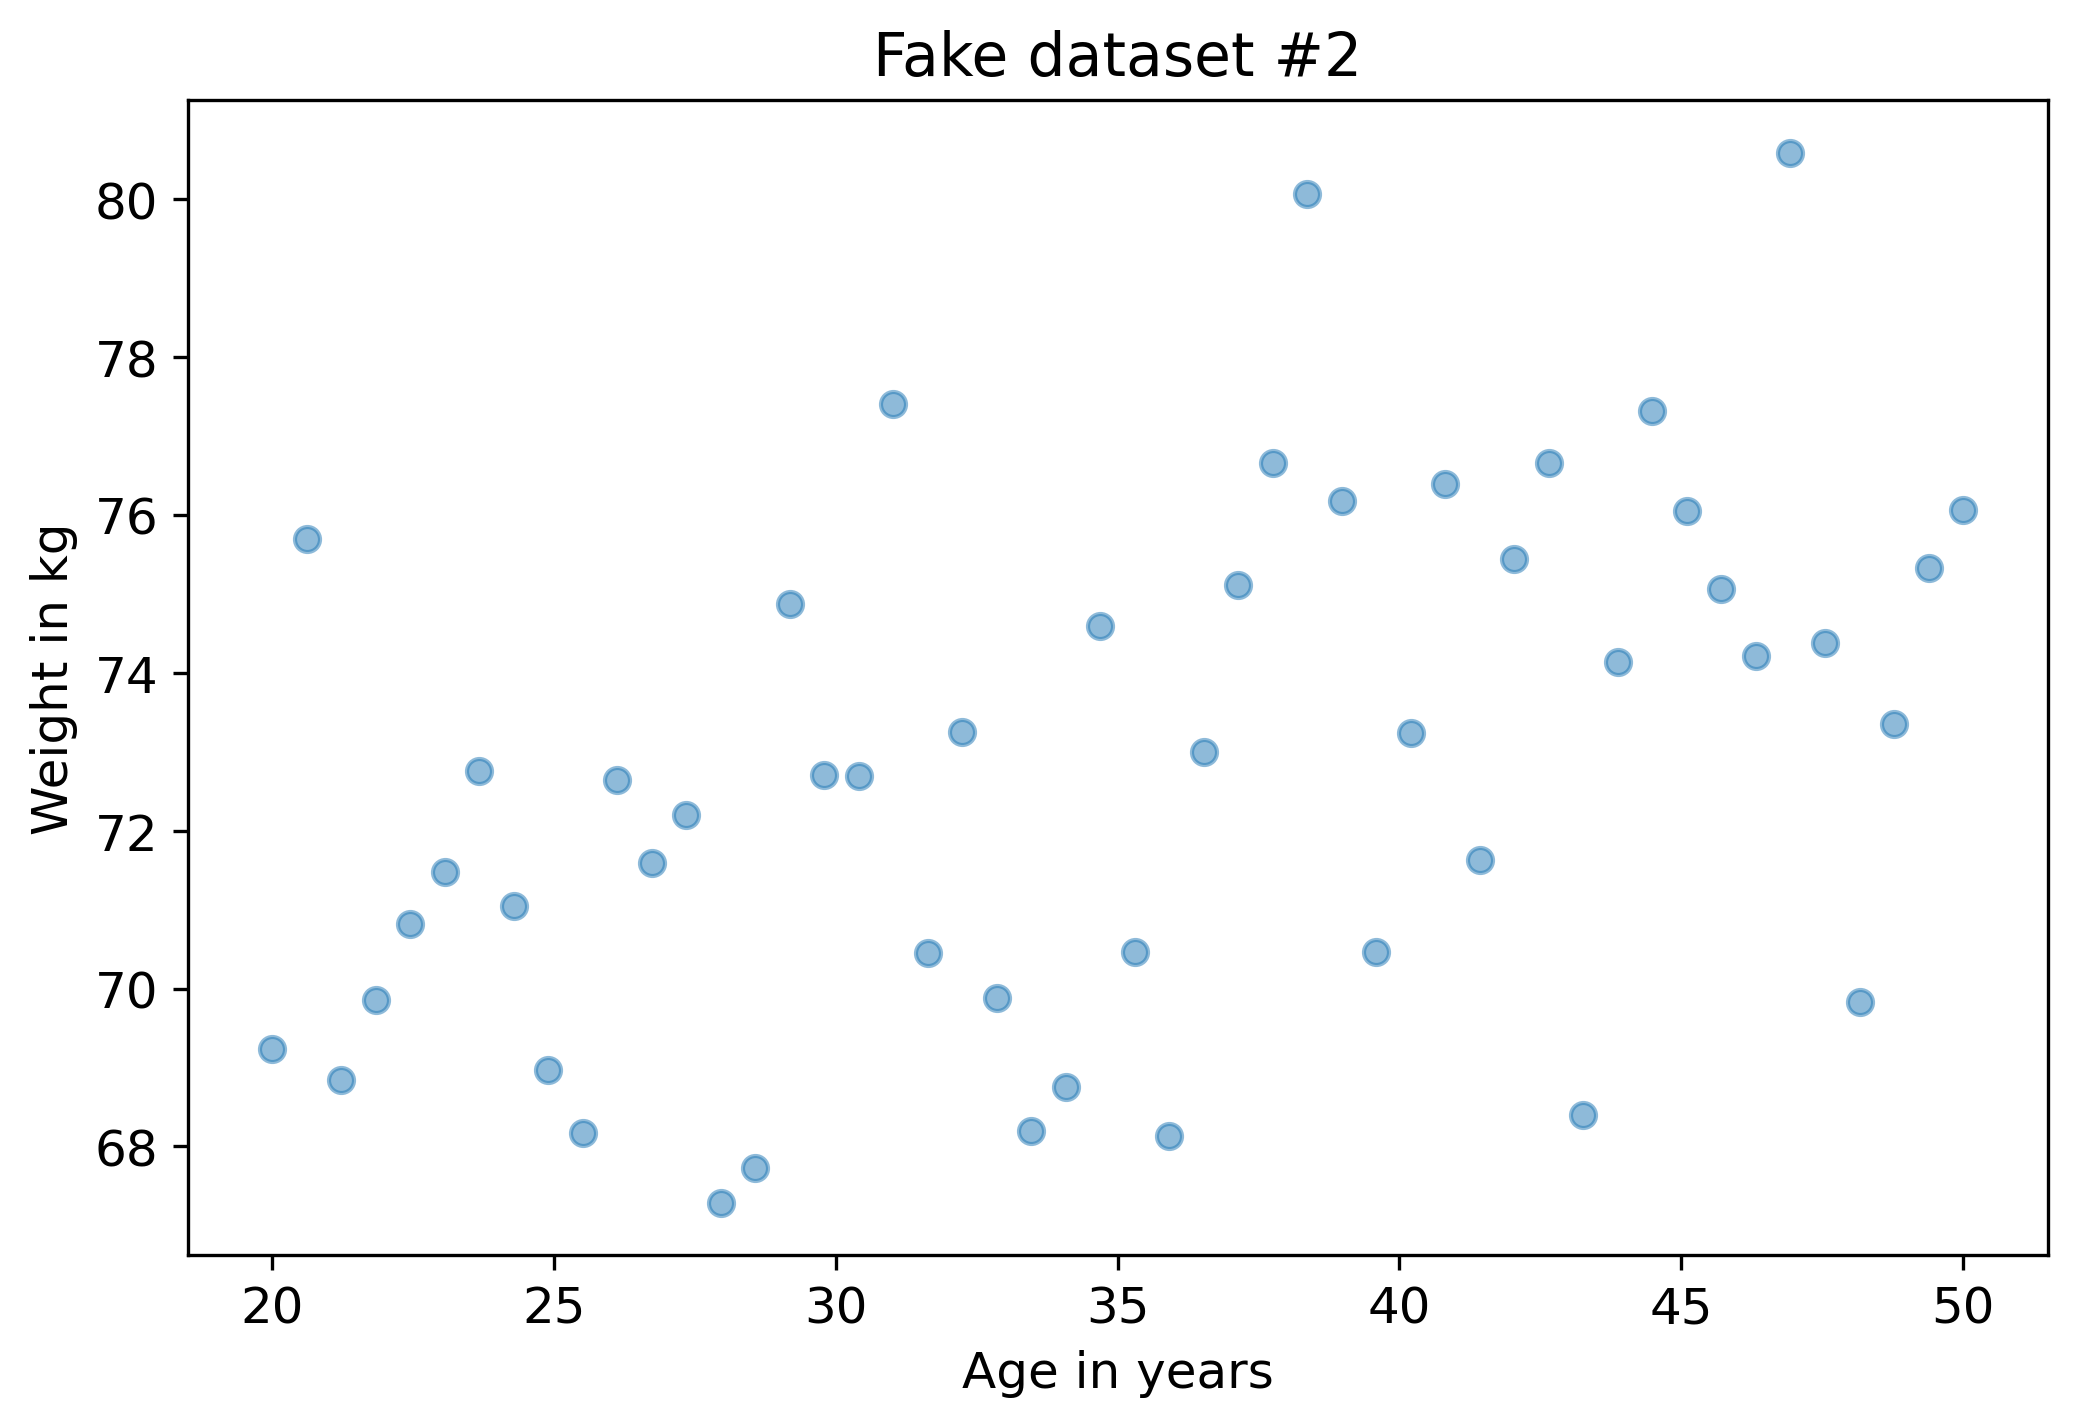
\includegraphics[width=4in]{chapters/09_relationships_files/09_relationships_68_0.png}
\end{center}

I constructed these examples so they look similar, but they have
substantially different correlations:

\begin{lstlisting}[]
rho1 = np.corrcoef(xs1, ys1)[0][1]
rho1
(@\dashfill@)
@@@0.7579660563439401@@@
\end{lstlisting}

\begin{lstlisting}[]
rho2 = np.corrcoef(xs2, ys2)[0][1]
rho2
(@\dashfill@)
@@@0.4782776976576317@@@
\end{lstlisting}

In the first example, the correlation is strong, close to
\passthrough{\lstinline!0.75!}. In the second example, the correlation
is moderate, close to \passthrough{\lstinline!0.5!}. So we might think
the first relationship is more important. But look more closely at the
\passthrough{\lstinline!y!} axis in both figures.

In the first example, the average weight gain over 30 years is less than
1 kilogram; in the second it is more than 5 kilograms! If we are
concerned about the health effects of weight gain, the second
relationship is probably more important, even though the correlation is
lower.\\
The statistic we really care about is the slope of the line, not the
coefficient of correlation.

In the next section, we'll see how to estimate that slope. But first,
let's practice with correlation.

\textbf{Exercise:} The purpose of the BRFSS is to explore health risk
factors, so it includes questions about diet. The column
\passthrough{\lstinline!\_VEGESU1!} represents the number of servings of
vegetables respondents reported eating per day.

Let's see how this variable relates to age and income.

\begin{itemize}

\item
  From the \passthrough{\lstinline!brfss!} DataFrame, select the columns
  \passthrough{\lstinline!'AGE'!}, \passthrough{\lstinline!INCOME2!},
  and \passthrough{\lstinline!\_VEGESU1!}.
\item
  Compute the correlation matrix for these variables.
\end{itemize}

\textbf{Exercise:} In the previous exercise, the correlation between
income and vegetable consumption is about
\passthrough{\lstinline!0.12!}. The correlation between age and
vegetable consumption is about \passthrough{\lstinline!-0.01!}.

Which of the following are correct interpretations of these results?

\begin{itemize}

\item
  \emph{A}: People in this dataset with higher incomes eat more
  vegetables.
\item
  \emph{B}: The relationship between income and vegetable consumption is
  linear.
\item
  \emph{C}: Older people eat more vegetables.
\item
  \emph{D}: There could be a strong non-linear relationship between age
  and vegetable consumption.
\end{itemize}

\textbf{Exercise:} In general it is a good idea to visualize the
relationship between variables \emph{before} you compute a correlation.
We didn't do that in the previous example, but it's not too late.

Generate a visualization of the relationship between age and vegetables.
How would you describe the relationship, if any?

\hypertarget{simple-linear-regression}{%
\section{Simple Linear Regression}\label{simple-linear-regression}}

In the previous section we saw that correlation does not always measure
what we really want to know. In this section, we look at an alternative:
simple linear regression.

Let's look again at the relationship between weight and age. In the
previous section, I generated two fake datasets to make a point:

\begin{lstlisting}[]
plt.figure(figsize=(8, 3))

plt.subplot(1, 2, 1)
plt.plot(xs1, ys1, 'o', alpha=0.5)
plt.xlabel('Age in years')
plt.ylabel('Weight in kg')
plt.title('Fake dataset #1')
plt.tight_layout()

plt.subplot(1, 2, 2)
plt.plot(xs2, ys2, 'o', alpha=0.5)
plt.xlabel('Age in years')
plt.ylabel('Weight in kg')
plt.title('Fake dataset #2')
plt.tight_layout()
\end{lstlisting}

\begin{center}
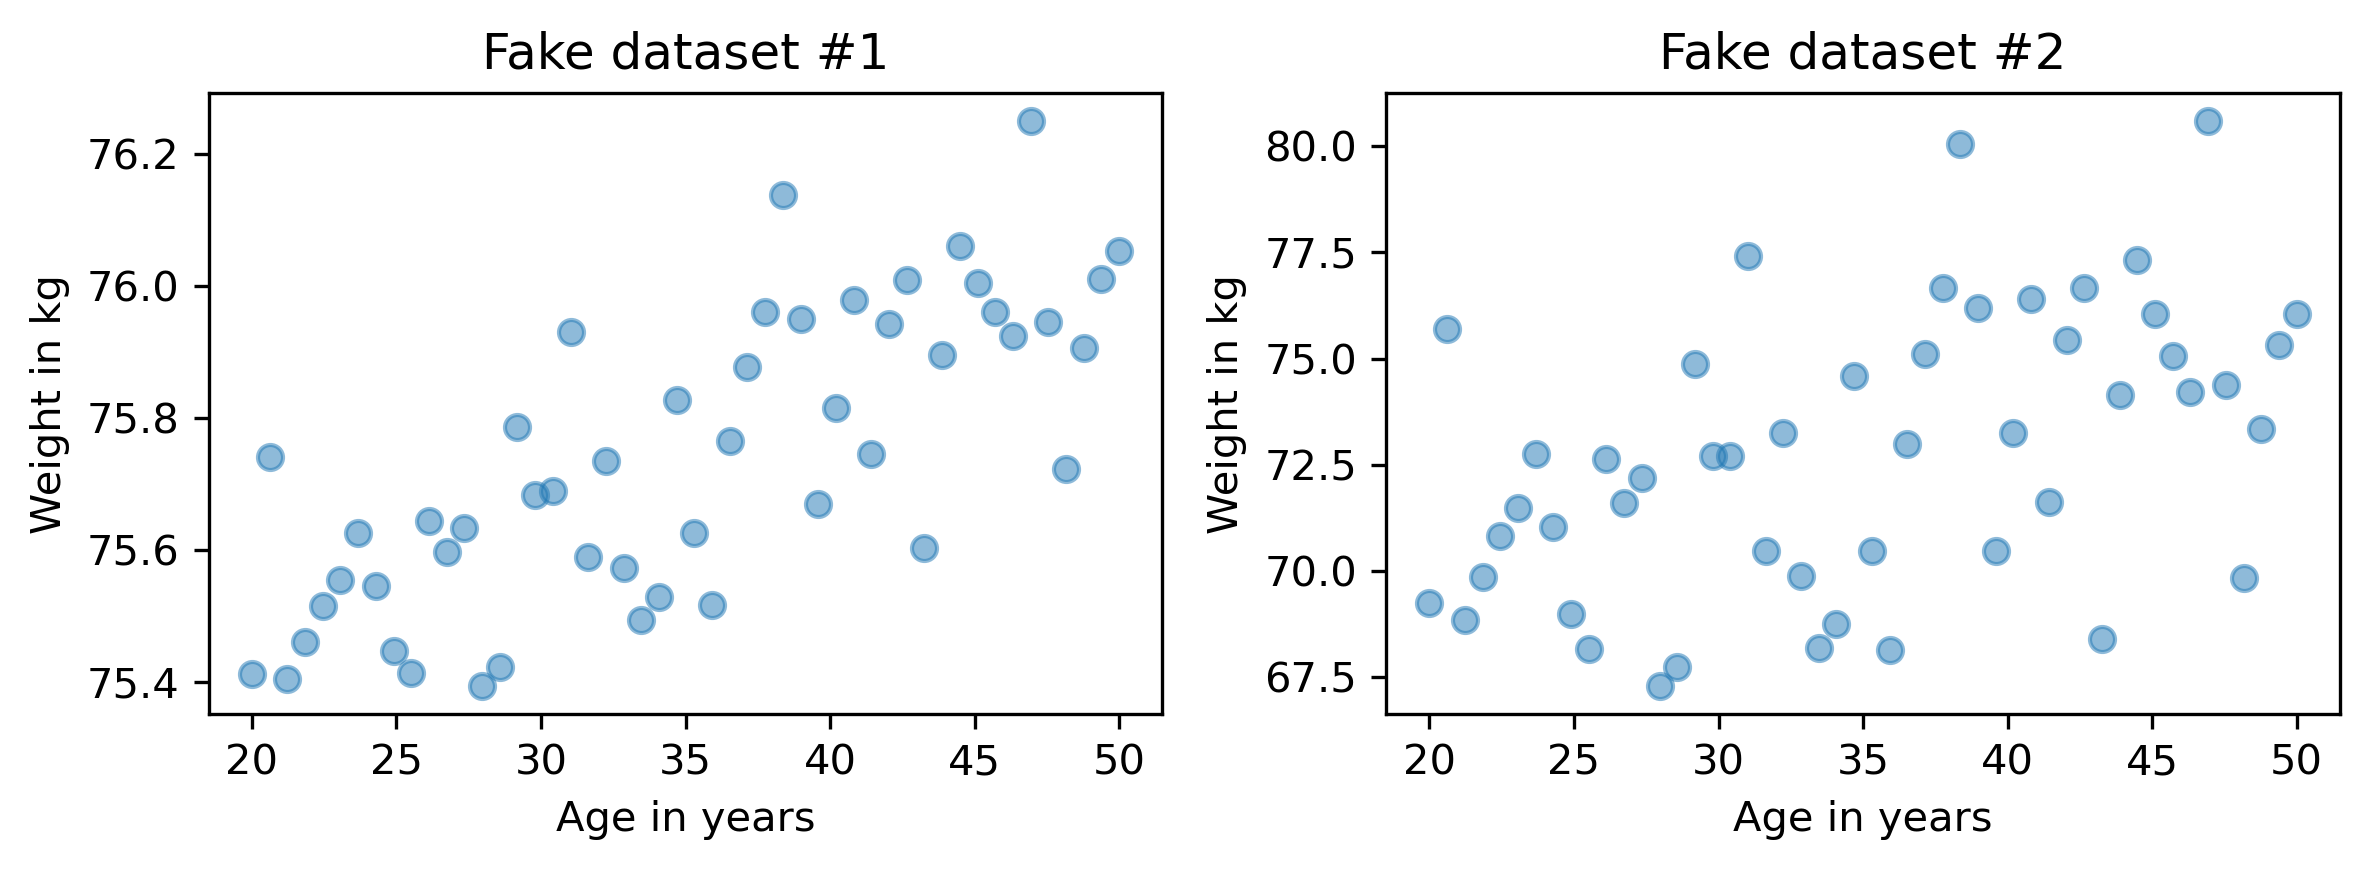
\includegraphics[width=4in]{chapters/09_relationships_files/09_relationships_77_0.png}
\end{center}

The one on the left has higher correlation, about 0.75 compared to 0.5.
But in this context, the statistic we probably care about is the slope
of the line, not the correlation coefficient. To estimate the slope, we
can use \passthrough{\lstinline!linregress!} from the SciPy
\passthrough{\lstinline!stats!} library.

\begin{lstlisting}[]
from scipy.stats import linregress

res1 = linregress(xs1, ys1)
res1._asdict()
(@\dashfill@)
@@@{'slope': 0.018821034903244386,
 'intercept': 75.08049023710964,
 'rvalue': 0.7579660563439402,
 'pvalue': 1.8470158725246148e-10,
 'stderr': 0.002337849260560818,
 'intercept_stderr': 0.08439154079040358}@@@
\end{lstlisting}

The result is a \passthrough{\lstinline!LinregressResult!} object that
contains five values: \passthrough{\lstinline!slope!} is the slope of
the line of best fit for the data; \passthrough{\lstinline!intercept!}
is the intercept. We'll interpret some of the other values later.

For Fake Dataset \#1, the estimated slope is about 0.019 kilograms per
year or about 0.56 kilograms over the 30-year range.

\begin{lstlisting}[]
res1.slope * 30
(@\dashfill@)
@@@0.5646310470973316@@@
\end{lstlisting}

Here are the results for Fake Dataset \#2.

\begin{lstlisting}[]
res2 = linregress(xs2, ys2)
res2._asdict()
(@\dashfill@)
@@@{'slope': 0.17642069806488855,
 'intercept': 66.60980474219305,
 'rvalue': 0.47827769765763173,
 'pvalue': 0.0004430600283776241,
 'stderr': 0.04675698521121631,
 'intercept_stderr': 1.6878308158080697}@@@
\end{lstlisting}

The estimated slope is almost 10 times higher: about 0.18 kilograms per
year or about 5.3 kilograms per 30 years:

\begin{lstlisting}[]
res2.slope * 30
(@\dashfill@)
@@@5.292620941946657@@@
\end{lstlisting}

What's called \passthrough{\lstinline!rvalue!} here is correlation,
which confirms what we saw before; the first example has higher
correlation, about 0.75 compared to 0.5. But the strength of the effect,
as measured by the slope of the line, is about 10 times higher in the
second example.

We can use the results from \passthrough{\lstinline!linregress!} to
compute the line of best fit: first we get the minimum and maximum of
the observed \passthrough{\lstinline!xs!}; then we multiply by the slope
and add the intercept. Here's what that looks like for the first
example.

\begin{lstlisting}[]
plt.plot(xs1, ys1, 'o', alpha=0.5)

fx = np.array([xs1.min(), xs1.max()])
fy = res1.intercept + res1.slope * fx
plt.plot(fx, fy, '-')

plt.xlabel('Age in years')
plt.ylabel('Weight in kg')
plt.title('Fake Dataset #1');
\end{lstlisting}

\begin{center}
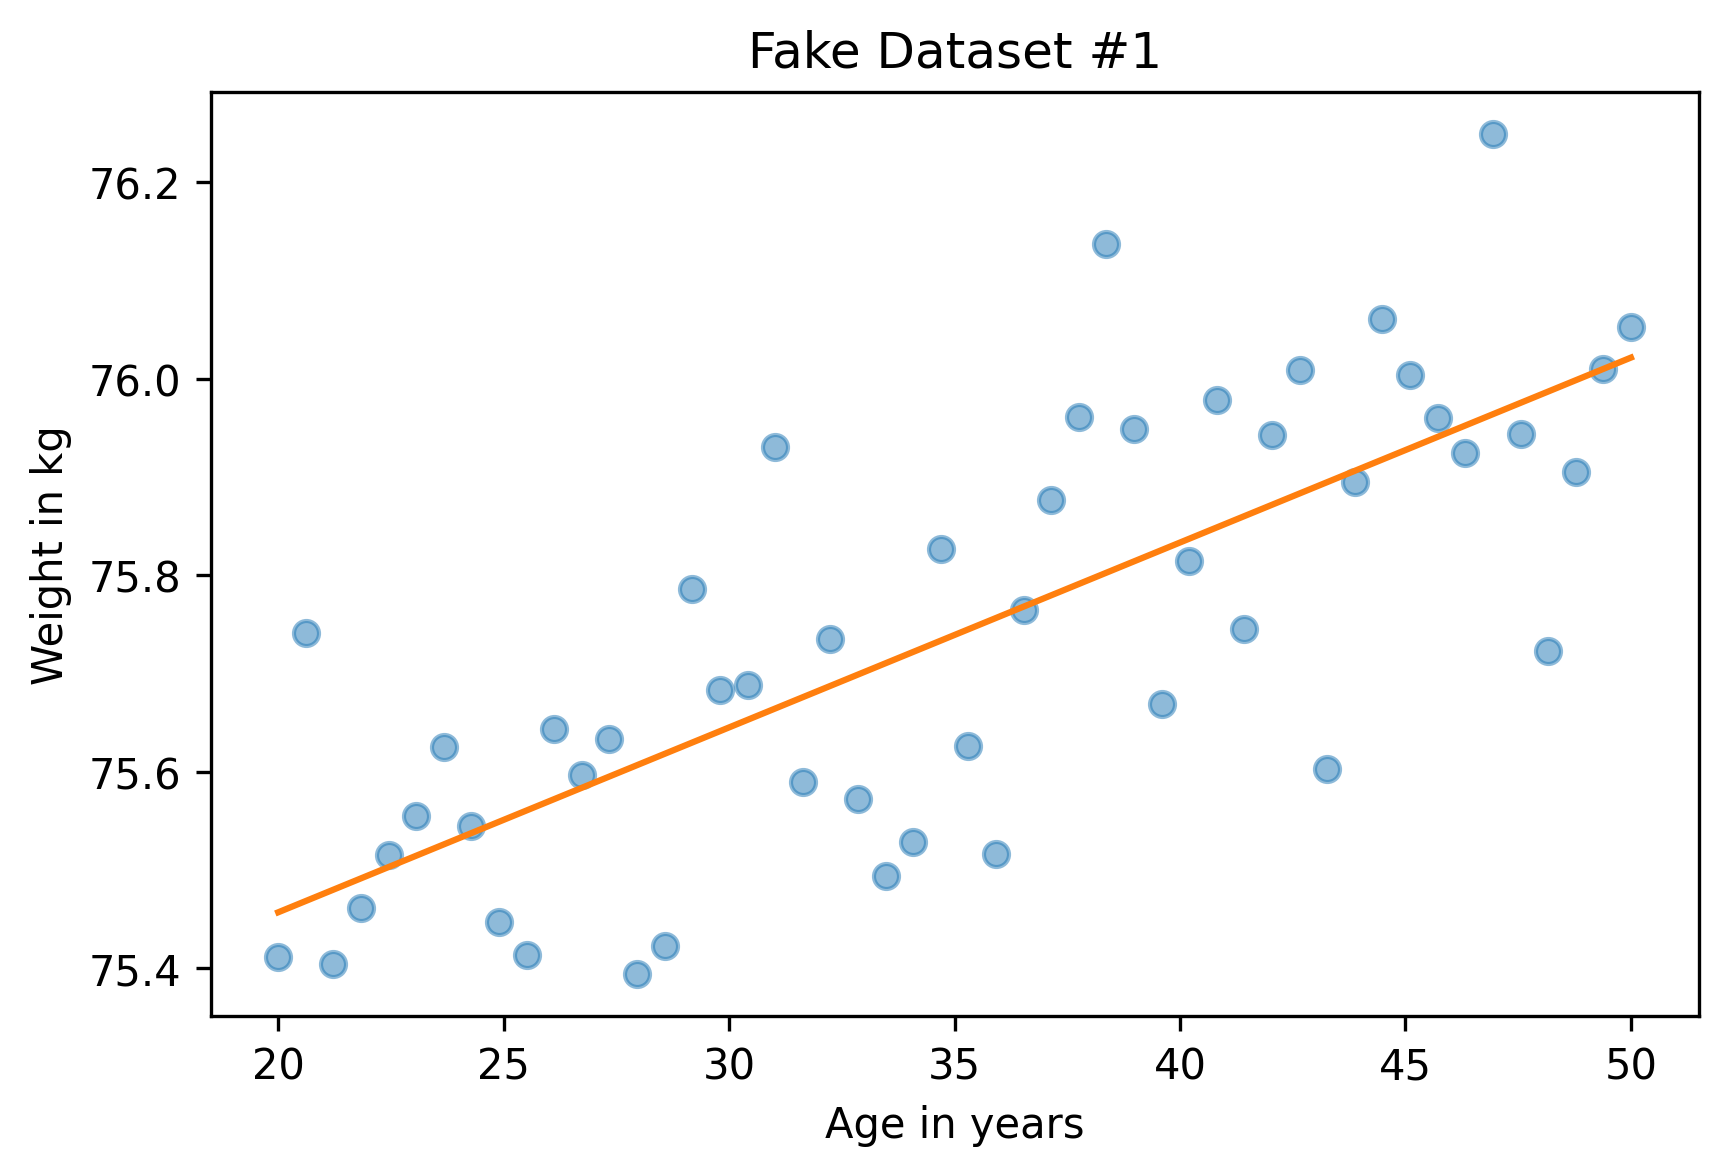
\includegraphics[width=4in]{chapters/09_relationships_files/09_relationships_87_0.png}
\end{center}

And here's what it looks like for the second example.

\begin{lstlisting}[]
plt.plot(xs2, ys2, 'o', alpha=0.5)

fx = np.array([xs2.min(), xs2.max()])
fy = res2.intercept + res2.slope * fx
plt.plot(fx, fy, '-')

plt.xlabel('Age in years')
plt.ylabel('Weight in kg')
plt.title('Fake Dataset #2');
\end{lstlisting}

\begin{center}
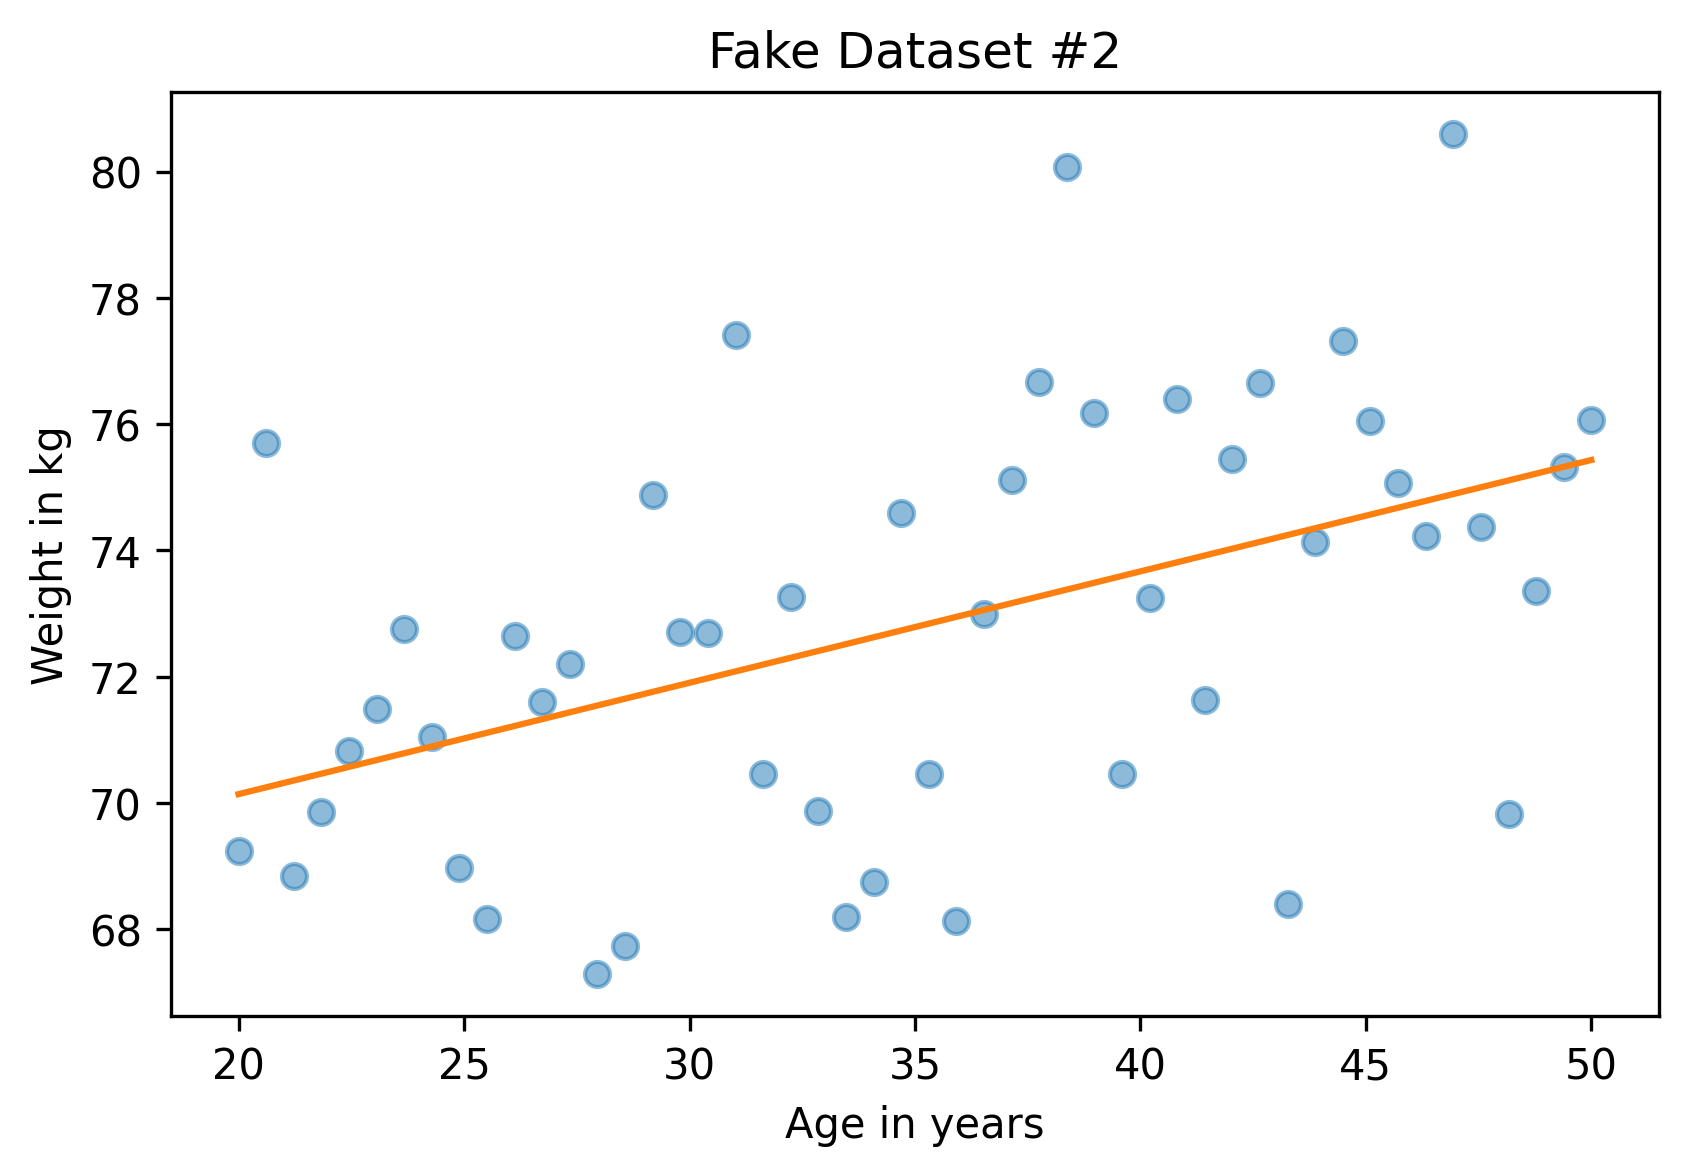
\includegraphics[width=4in]{chapters/09_relationships_files/09_relationships_89_0.png}
\end{center}

The visualization here might be misleading unless you look closely at
the vertical scales; the slope in the second figure is almost 10 times
higher.

\hypertarget{regression-of-height-and-weight}{%
\section{Regression of Height and
Weight}\label{regression-of-height-and-weight}}

Now let's look at an example of regression with real data. Here's the
scatter plot of height and weight one more time.

\begin{lstlisting}[]
plt.plot(height_jitter, weight_jitter, 'o', 
         alpha=0.02, markersize=1)

plt.xlim([140, 200])
plt.ylim([0, 160])
plt.xlabel('Height in cm')
plt.ylabel('Weight in kg')
plt.title('Scatter plot of weight versus height');
\end{lstlisting}

\begin{center}
\includegraphics[width=4in]{chapters/09_relationships_files/09_relationships_92_0.png}
\end{center}

To compute the regression line, we'll use
\passthrough{\lstinline!linregress!} again. But it can't handle
\passthrough{\lstinline!NaN!} values, so we have to use
\passthrough{\lstinline!dropna!} to remove rows that are missing the
data we need.

\begin{lstlisting}[]
subset = brfss.dropna(subset=['WTKG3', 'HTM4'])
height_clean = subset['HTM4']
weight_clean = subset['WTKG3']
\end{lstlisting}

Now we can compute the linear regression.

\begin{lstlisting}[]
res_hw = linregress(height_clean, weight_clean)
res_hw._asdict()
(@\dashfill@)
@@@{'slope': 0.9192115381848305,
 'intercept': -75.12704250330248,
 'rvalue': 0.4742030897902462,
 'pvalue': 0.0,
 'stderr': 0.005632863769802998,
 'intercept_stderr': 0.9608860265433182}@@@
\end{lstlisting}

The slope is about 0.92 kilograms per centimeter, which means that we
expect a person one centimeter taller to be almost a kilogram heavier.
That's quite a lot.

As before, we can compute the line of best fit:

\begin{lstlisting}[]
fx = np.array([height_clean.min(), height_clean.max()])
fy = res_hw.intercept + res_hw.slope * fx
\end{lstlisting}

And here's what that looks like.

\begin{lstlisting}[]
plt.plot(height_jitter, weight_jitter, 'o', alpha=0.02, markersize=1)

plt.plot(fx, fy, '-')

plt.xlim([140, 200])
plt.ylim([0, 160])
plt.xlabel('Height in cm')
plt.ylabel('Weight in kg')
plt.title('Scatter plot of weight versus height');
\end{lstlisting}

\begin{center}
\includegraphics[width=4in]{chapters/09_relationships_files/09_relationships_100_0.png}
\end{center}

The slope of this line seems consistent with the scatter plot.

Linear regression has the same problem as correlation; it only measures
the strength of a linear relationship. Here's the scatter plot of weight
versus age, which we saw earlier.

\begin{lstlisting}[]
plt.plot(age_jitter, weight_jitter, 'o', 
         alpha=0.01, markersize=1)

plt.ylim([0, 160])
plt.xlabel('Age in years')
plt.ylabel('Weight in kg')
plt.title('Weight versus age');
\end{lstlisting}

\begin{center}
\includegraphics[width=4in]{chapters/09_relationships_files/09_relationships_102_0.png}
\end{center}

People in their 40s are the heaviest; younger and older people are
lighter. So the relationship is nonlinear.

If we don't look at the scatter plot and blindly compute the regression
line, here's what we get.

\begin{lstlisting}[]
subset = brfss.dropna(subset=['WTKG3', 'AGE'])
age_clean = subset['AGE']
weight_clean = subset['WTKG3']

res_aw = linregress(age_clean, weight_clean)
res_aw._asdict()
(@\dashfill@)
@@@{'slope': 0.023981159566968734,
 'intercept': 80.07977583683224,
 'rvalue': 0.02164143288906408,
 'pvalue': 4.374327493007456e-11,
 'stderr': 0.003638139410742185,
 'intercept_stderr': 0.1868850817687016}@@@
\end{lstlisting}

The estimated slope is only 0.02 kilograms per year, or 0.6 kilograms in
30 years. And here's what the line of best fit looks like.

\begin{lstlisting}[]
plt.plot(age_jitter, weight_jitter, 'o', 
         alpha=0.01, markersize=1)

fx = np.array([age_clean.min(), age_clean.max()])
fy = res_aw.intercept + res_aw.slope * fx
plt.plot(fx, fy, '-')

plt.ylim([0, 160])
plt.xlabel('Age in years')
plt.ylabel('Weight in kg')
plt.title('Weight versus age');
\end{lstlisting}

\begin{center}
\includegraphics[width=4in]{chapters/09_relationships_files/09_relationships_106_0.png}
\end{center}

A straight line does not capture the relationship between these
variables well.

In the next chapter, you'll see how to use multiple regression to
estimate non-linear relationships. But first, let's practice simple
regression.

\textbf{Exercise:} Who do you think eats more vegetables, people with
low income, or people with high income? Let's find out.

As we've seen previously, the column \passthrough{\lstinline!INCOME2!}
represents income level and \passthrough{\lstinline!\_VEGESU1!}
represents the number of vegetable servings respondents reported eating
per day.

Make a scatter plot with vegetable servings versus income, that is, with
vegetable servings on the \passthrough{\lstinline!y!} axis and income
group on the \passthrough{\lstinline!x!} axis.

You might want to use \passthrough{\lstinline!ylim!} to zoom in on the
bottom half of the \passthrough{\lstinline!y!} axis.

\textbf{Exercise:} Now let's estimate the slope of the relationship
between vegetable consumption and income.

\begin{itemize}
\item
  Use \passthrough{\lstinline!dropna!} to select rows where
  \passthrough{\lstinline!INCOME2!} and
  \passthrough{\lstinline!\_VEGESU1!} are not
  \passthrough{\lstinline!NaN!}.
\item
  Extract \passthrough{\lstinline!INCOME2!} and
  \passthrough{\lstinline!\_VEGESU1!} and compute the simple linear
  regression of these variables.
\end{itemize}

What is the slope of the regression line? What does this slope means in
the context of the question we are exploring?

\textbf{Exercise:} Finally, plot the regression line on top of the
scatter plot.

\hypertarget{summary}{%
\section{Summary}\label{summary}}

This chapter presents three ways to visualize the relationship between
two variables: a scatter plot, violin plot, and box plot. A scatter plot
is often a good choice when you are exploring a new data set, but it can
take some attention to avoid overplotting. Violin and box plot are
particularly useful when one of the variables only takes on a few
discrete values.

And we considered two ways to quantify the strength of a relationship:
the coefficient of correlation and the slope of a regression line. These
statistics capture different aspect of what we might mean by
``strength''. The coefficient of correlation indicates how well we can
predict one variable, given the other. The slope of the regression line
indicates how much difference we expect in one variable as we vary the
other. One or the other might be more relevant, depending on the
context.



\chapter{Regression}\label{regression}

In the previous chapter we used simple linear regression to quantify the
relationship between two variables. In this chapter we'll get farther
into regression, including multiple regression and one of my all-time
favorite tools, logistic regression. These tools will allow us to
explore relationships among sets of variables. As an example, we will
use data from the General Social Survey (GSS) to explore the
relationship between education, sex, age, and income.

The GSS dataset contains hundreds of columns. We'll work with an extract
that contains just the columns we need, as we did in Chapter 8.
Instructions for downloading the extract are in the notebook for this
chapter.
\index{General Social Survey}
\index{GSS}


We can read the \passthrough{\lstinline!DataFrame!} like this and
display the first few rows.

\begin{lstlisting}[language=Python,style=source]
import pandas as pd

gss = pd.read_hdf('gss_extract_2022.hdf', 'gss')
gss.head()
\end{lstlisting}

\begin{tabular}{lrrrrrrrrr}
\toprule
 & year & id & age & educ & degree & sex & gunlaw & grass & realinc \\
\midrule
0 & 1972 & 1 & 23 & 16 & 3 & 2 & 1 & NaN & 18951 \\
1 & 1972 & 2 & 70 & 10 & 0 & 1 & 1 & NaN & 24366 \\
2 & 1972 & 3 & 48 & 12 & 1 & 2 & 1 & NaN & 24366 \\
3 & 1972 & 4 & 27 & 17 & 3 & 2 & 1 & NaN & 30458 \\
4 & 1972 & 5 & 61 & 12 & 1 & 2 & 1 & NaN & 50763 \\
\bottomrule
\end{tabular}

We'll start with a simple regression, estimating the parameters of real
income as a function of years of education.
\index{simple regression}
\index{education}
\index{income}

\pagebreak

First we'll select the subset of the data where both variables are valid.
\index{dropna (Pandas method)}

\begin{lstlisting}[language=Python,style=source]
data = gss.dropna(subset=['realinc', 'educ'])
xs = data['educ']
ys = data['realinc']
\end{lstlisting}

Now we can use \passthrough{\lstinline!linregress!} to fit a line to the
data.
\index{linregress (SciPy function)}

\begin{lstlisting}[language=Python,style=source]
from scipy.stats import linregress
res = linregress(xs, ys)
res._asdict()
\end{lstlisting}

\begin{lstlisting}[style=output]
{'slope': 3631.0761003894995,
 'intercept': -15007.453640508655,
 'rvalue': 0.37169252259280877,
 'pvalue': 0.0,
 'stderr': 35.625290800764,
 'intercept_stderr': 480.07467595184363}
\end{lstlisting}

The estimated slope is about 3450, which means that each additional year
of education is associated with an additional \$3450 of income.
\index{slope}

\section{Regression with StatsModels}\label{regression-with-statsmodels}

SciPy doesn't do multiple regression, so we'll to switch to a new
library, StatsModels. Here's the import statement.
\index{StatsModels library}

\begin{lstlisting}[language=Python,style=source]
import statsmodels.formula.api as smf
\end{lstlisting}

To fit a regression model, we'll use \passthrough{\lstinline!ols!},
which stands for ``ordinary least squares'', another name for
regression.
\index{ordinary least squares}
\index{ols (StatsModels function)}
\index{fit (StatsModels function)}


\begin{lstlisting}[language=Python,style=source]
results = smf.ols('realinc ~ educ', data=data).fit()
\end{lstlisting}

The first argument is a \textbf{formula string} that specifies that we
want to regress income as a function of education. The second argument
is the \passthrough{\lstinline!DataFrame!} containing the subset of
valid data. The names in the formula string correspond to columns in the
\passthrough{\lstinline!DataFrame!}.
\index{formula string}

The result from \passthrough{\lstinline!ols!} is an object that
represents the model -- it provides a function called
\passthrough{\lstinline!fit!} that does the actual computation.

\pagebreak

The result from \passthrough{\lstinline!fit!} is a \passthrough{\lstinline!RegressionResultsWrapper!},
which contains a \passthrough{\lstinline!Series!} called
\passthrough{\lstinline!params!}, which contains the estimated intercept
and the slope associated with \passthrough{\lstinline!educ!}.
\index{slope}
\index{intercept}


\begin{lstlisting}[language=Python,style=source]
results.params
\end{lstlisting}

\begin{lstlisting}[style=output]
Intercept   -15007.453641
educ          3631.076100
dtype: float64
\end{lstlisting}

The results from Statsmodels are the same as the results we got from
SciPy, so that's good!

\textbf{Exercise:} Let's run another regression using SciPy and
StatsModels, and confirm we get the same results. Compute the regression
of \passthrough{\lstinline!realinc!} as a function of
\passthrough{\lstinline!age!} using SciPy's
\passthrough{\lstinline!linregress!} and then using StatsModels'
\passthrough{\lstinline!ols!}. Confirm that the intercept and slope are
the same. Remember to use \passthrough{\lstinline!dropna!} to select the
rows with valid data in both columns.

\section{Multiple Regression}\label{multiple-regression}

In the previous section, we saw that income depends on education, and in
the exercise we saw that it also depends on
\passthrough{\lstinline!age!}. Now let's put them together in a single
model.
\index{multiple regression}
\index{income}
\index{age}


\begin{lstlisting}[language=Python,style=source]
results = smf.ols('realinc ~ educ + age', data=gss).fit()
results.params
\end{lstlisting}

\begin{lstlisting}[style=output]
Intercept   -17999.726908
educ          3665.108238
age             55.071802
dtype: float64
\end{lstlisting}

In this model, \passthrough{\lstinline!realinc!} is the variable we are
trying to explain or predict, which is called the \textbf{dependent
variable} because it depends on the the other variables -- or at least
we expect it to. The other variables, \passthrough{\lstinline!educ!} and
\passthrough{\lstinline!age!}, are called \textbf{independent variables}
or sometimes ``predictors''. The \passthrough{\lstinline!+!} sign
indicates that we expect the contributions of the independent variables
to be additive.
\index{predictor}
\index{independent variable}
\index{dependent variable}

The result contains an intercept and two slopes, which estimate the
average contribution of each predictor with the other predictor held
constant.

\begin{itemize}
\item
  The estimated slope for \passthrough{\lstinline!educ!} is about 3665
  -- so if we compare two people with the same age, and one has an
  additional year of education, we expect their income to be higher by
  \$3514.
\item
  The estimated slope for \passthrough{\lstinline!age!} is about 55 --
  so if we compare two people with the same education, and one is a year
  older, we expect their income to be higher by \$55.
\end{itemize}

In this model, the contribution of age is quite small, but as we'll see
in the next section that might be misleading.

\section{Grouping by Age}\label{grouping-by-age}

Let's look more closely at the relationship between income and age.
We'll use a Pandas method we have not seen before, called
\passthrough{\lstinline!groupby!}, to divide the
\passthrough{\lstinline!DataFrame!} into age groups.
\index{groupby (Pandas method)}

\begin{lstlisting}[language=Python,style=source]
grouped = gss.groupby('age')
type(grouped)
\end{lstlisting}

\begin{lstlisting}[style=output]
pandas.core.groupby.generic.DataFrameGroupBy
\end{lstlisting}

The result is a \passthrough{\lstinline!GroupBy!} object that contains
one group for each value of \passthrough{\lstinline!age!}. The
\passthrough{\lstinline!GroupBy!} object behaves like a
\passthrough{\lstinline!DataFrame!} in many ways. You can use brackets
to select a column, like \passthrough{\lstinline!realinc!} in this
example, and then invoke a method like \passthrough{\lstinline!mean!}.
\index{DataFrameGroupBy object}
\index{mean (Pandas method)}
\index{bracket operator}

\begin{lstlisting}[language=Python,style=source]
mean_income_by_age = grouped['realinc'].mean()
\end{lstlisting}

The result is a Pandas \passthrough{\lstinline!Series!} that contains
the mean income for each age group, which we can plot like this.

\begin{lstlisting}[language=Python,style=source]
import matplotlib.pyplot as plt

plt.plot(mean_income_by_age, 'o', alpha=0.5)
plt.xlabel('Age (years)')
plt.ylabel('Income (1986 $)')
plt.title('Average income, grouped by age');
\end{lstlisting}

\begin{center}
\includegraphics[scale=0.6666666]{10_regression_files/10_regression_31_0.png}
\end{center}

Average income increases from age 20 to age 50, then starts to fall. And
that explains why the estimated slope is so small, because the
relationship is nonlinear.
\index{nonlinear relationship}

\pagebreak

To describe a nonlinear relationship, we'll
create a new variable called \passthrough{\lstinline!age2!} that equals
\passthrough{\lstinline!age!} squared -- so it is called a
\textbf{quadratic term}.
\index{quadratic term}

\begin{lstlisting}[language=Python,style=source]
gss['age2'] = gss['age']**2
\end{lstlisting}

Now we can run a regression with both \passthrough{\lstinline!age!} and
\passthrough{\lstinline!age2!} on the right side.

\begin{lstlisting}[language=Python,style=source]
model = smf.ols('realinc ~ educ + age + age2', data=gss)
results = model.fit()
results.params
\end{lstlisting}

\begin{lstlisting}[style=output]
Intercept   -52599.674844
educ          3464.870685
age           1779.196367
age2           -17.445272
dtype: float64
\end{lstlisting}

In this model, the slope associated with \passthrough{\lstinline!age!}
is substantial, about \$1779 per year.

The slope associated with \passthrough{\lstinline!age2!} is about -\$17.
It might be unexpected that it is negative -- we'll see why in the next
section. But first, here are two exercises where you can practice using
\passthrough{\lstinline!groupby!} and \passthrough{\lstinline!ols!}.

\textbf{Exercise:} Let's explore the relationship between income and
education. First, group \passthrough{\lstinline!gss!} by
\passthrough{\lstinline!educ!}. From the resulting
\passthrough{\lstinline!GroupBy!} object, extract
\passthrough{\lstinline!realinc!} and compute the mean. Then plot mean
income in each education group. What can you say about the relationship
between these variables? Does it look like a linear relationship?

\textbf{Exercise:} The graph in the previous exercise suggests that the
relationship between income and education is nonlinear. So let's try
fitting a nonlinear model.

\begin{itemize}
\item
  Add a column named \passthrough{\lstinline!educ2!} to the
  \passthrough{\lstinline!gss!} DataFrame -- it should contain the
  values from \passthrough{\lstinline!educ!} squared.
\item
  Run a regression that uses \passthrough{\lstinline!educ!},
  \passthrough{\lstinline!educ2!}, \passthrough{\lstinline!age!}, and
  \passthrough{\lstinline!age2!} to predict
  \passthrough{\lstinline!realinc!}.
\end{itemize}

\section{Visualizing regression
results}\label{visualizing-regression-results}

In the previous section we ran a multiple regression model to
characterize the relationships between income, age, and education.
Because the model includes quadratic terms, the parameters are hard to
interpret. For example, you might notice that the parameter for
\passthrough{\lstinline!educ!} is negative, and that might be a
surprise, because it suggests that higher education is associated with
lower income. But the parameter for \passthrough{\lstinline!educ2!} is
positive, and that makes a big difference. In this section we'll see a
way to interpret the model visually and validate it against data.

\pagebreak

Here's the model from the previous exercise.

\begin{lstlisting}[language=Python,style=source]
gss['educ2'] = gss['educ']**2

model = smf.ols('realinc ~ educ + educ2 + age + age2', data=gss)
results = model.fit()
results.params
\end{lstlisting}

\begin{lstlisting}[style=output]
Intercept   -26336.766346
educ          -706.074107
educ2          165.962552
age           1728.454811
age2           -17.207513
dtype: float64
\end{lstlisting}

The \passthrough{\lstinline!results!} object provides a method called
\passthrough{\lstinline!predict!} that uses the estimated parameters to
generate predictions. It takes a \passthrough{\lstinline!DataFrame!} as
a parameter and returns a \passthrough{\lstinline!Series!} with a
prediction for each row in the \passthrough{\lstinline!DataFrame!}. To
use it, we'll create a new \passthrough{\lstinline!DataFrame!} with
\passthrough{\lstinline!age!} running from 18 to 89, and
\passthrough{\lstinline!age2!} set to \passthrough{\lstinline!age!}
squared.

\begin{lstlisting}[language=Python,style=source]
import numpy as np

df = pd.DataFrame()
df['age'] = np.linspace(18, 89)
df['age2'] = df['age']**2
\end{lstlisting}

Next, we'll pick a level for \passthrough{\lstinline!educ!}, like 12
years, which is the most common value. When you assign a single value to
a column in a \passthrough{\lstinline!DataFrame!}, Pandas makes a copy
for each row.

\begin{lstlisting}[language=Python,style=source]
df['educ'] = 12
df['educ2'] = df['educ']**2
\end{lstlisting}

Then we can use \passthrough{\lstinline!results!} to predict the average
income for each age group, holding education constant.
\index{predict (StatsModels method)}

\begin{lstlisting}[language=Python,style=source]
pred12 = results.predict(df)
\end{lstlisting}

The result from \passthrough{\lstinline!predict!} is a
\passthrough{\lstinline!Series!} with one prediction for each row. So we
can plot it with age on the x-axis and the predicted income for each age
group on the y-axis. And we'll plot the data for comparison.

\pagebreak

\begin{lstlisting}[language=Python,style=source]
plt.plot(mean_income_by_age, 'o', alpha=0.5)
plt.plot(df['age'], pred12, label='High school', color='C4')

plt.xlabel('Age (years)')
plt.ylabel('Income (1986 $)')
plt.title('Income versus age, grouped by education level')
plt.legend();
\end{lstlisting}

\begin{center}
\includegraphics[scale=0.6666666]{10_regression_files/10_regression_48_0.png}
\end{center}

The dots show the average income in each age group. The line shows the
predictions generated by the model, holding education constant. This
plot shows the shape of the model, a downward-facing parabola.
\index{parabola}

We can do the same thing with other levels of education, like 14 years,
which is the nominal time to earn an Associate's degree, and 16 years,
which is the nominal time to earn a Bachelor's degree.

\begin{lstlisting}[language=Python,style=source]
df['educ'] = 16
df['educ2'] = df['educ']**2
pred16 = results.predict(df)

df['educ'] = 14
df['educ2'] = df['educ']**2
pred14 = results.predict(df)
\end{lstlisting}

\pagebreak

\begin{lstlisting}[language=Python,style=source]
plt.plot(mean_income_by_age, 'o', alpha=0.5)
plt.plot(df['age'], pred16, ':', label='Bachelor')
plt.plot(df['age'], pred14, '--', label='Associate')
plt.plot(df['age'], pred12, label='High school', color='C4')

plt.xlabel('Age (years)')
plt.ylabel('Income (1986 $)')
plt.title('Income versus age, grouped by education level')
plt.legend();
\end{lstlisting}

\begin{center}
\includegraphics[scale=0.6666666]{10_regression_files/10_regression_51_0.png}
\end{center}

The lines show expected income as a function of age for three levels of
education. This visualization helps validate the model, since we can
compare the predictions with the data. And it helps us interpret the
model since we can see the separate contributions of age and education.

Sometimes we can understand a model by looking at its parameters, but
often it is better to look at its predictions. In the exercises, you'll
have a chance to run a multiple regression, generate predictions, and
visualize the results.

\textbf{Exercise:} At this point, we have a model that predicts income
using age and education, and we've plotted predictions for different age
groups, holding education constant. Now let's see what it predicts for
different levels of education, holding age constant.

\begin{itemize}
\item
  Create an empty \passthrough{\lstinline!DataFrame!} named
  \passthrough{\lstinline!df!}.
\item
  Using \passthrough{\lstinline!np.linspace()!}, add a column named
  \passthrough{\lstinline!educ!} to \passthrough{\lstinline!df!} with a
  range of values from \passthrough{\lstinline!0!} to
  \passthrough{\lstinline!20!}.
\item
  Add a column named \passthrough{\lstinline!educ2!} with the values
  from \passthrough{\lstinline!educ!} squared.
\item
  Add a column named \passthrough{\lstinline!age!} with the constant
  value \passthrough{\lstinline!30!}.
\item
  Add a column named \passthrough{\lstinline!age2!} with the values from
  \passthrough{\lstinline!age!} squared.
\item
  Use the \passthrough{\lstinline!results!} object and
  \passthrough{\lstinline!df!} to generate expected income as a function
  of education.
\end{itemize}

\textbf{Exercise:} Now let's visualize the results from the previous
exercise.

\begin{itemize}
\item
  Group the GSS data by \passthrough{\lstinline!educ!} and compute the
  mean income in each education group.
\item
  Plot mean income for each education group as a scatter plot.
\item
  Plot the predictions from the previous exercise.
\end{itemize}

How do the predictions compare with the data?

\section{Categorical Variables}\label{categorical-variables}

Most of the variables we have used so far -- like income, age, and
education -- are numerical. But variables like sex and race are
\textbf{categorical} -- that is, each respondent belongs to one of a
specified set of categories. If there are only two categories, the
variable is \textbf{binary}.
\index{categorical variable}
\index{binary variable}


With StatsModels, it is easy to include a categorical variable as part
of a regression model. Here's an example:

\begin{lstlisting}[language=Python,style=source]
formula = 'realinc ~ educ + educ2 + age + age2 + C(sex)'
results = smf.ols(formula, data=gss).fit()
results.params
\end{lstlisting}

\begin{lstlisting}[style=output]
Intercept       -24635.767539
C(sex)[T.2.0]    -4891.439306
educ              -496.623120
educ2              156.898221
age               1720.274097
age2               -17.097853
dtype: float64
\end{lstlisting}

In the formula string, the letter \passthrough{\lstinline!C!} indicates
that \passthrough{\lstinline!sex!} is a categorical variable. The
regression treats the value \passthrough{\lstinline!sex=1!}, which is
male, as the reference group, and reports the difference associated with
the value \passthrough{\lstinline!sex=2!}, which is female. So the
results indicate that income for women is about \$4156 less than for
men, after controlling for age and education. However, note that
\passthrough{\lstinline!realinc!} represents household income. If the
respondent is married, it includes both their own income and their
spouse's. So we cannot interpret this result as an estimate of a gender
gap in income.

\section{Logistic Regression}\label{logistic-regression}

In the previous section, we added a categorical variable on the right
side of a regression formula -- that is, we used it as a predictive
variable.
\index{logistic regression}

But what if the categorical variable is on the left side of the
regression formula -- that is, it's the value we are trying to predict?
In that case, we can use \textbf{logistic regression}.

As an example, one of the GSS questions asks ``Would you favor or oppose
a law which would require a person to obtain a police permit before he
or she could buy a gun?'' The responses are in a column called
\passthrough{\lstinline!gunlaw!} -- here are the values.
\index{gun control}

\begin{lstlisting}[language=Python,style=source]
gss['gunlaw'].value_counts()
\end{lstlisting}

\begin{lstlisting}[style=output]
gunlaw
1.0    36367
2.0    11940
Name: count, dtype: int64
\end{lstlisting}

\passthrough{\lstinline!1!} means yes and \passthrough{\lstinline!2!}
means no, so most respondents are in favor.
\index{sex}

Before we can use this variable in a logistic regression, we have to
recode it so \passthrough{\lstinline!1!} means ``yes'' and
\passthrough{\lstinline!0!} means ``no''. We can do that by replacing
\passthrough{\lstinline!2!} with \passthrough{\lstinline!0!}.

\begin{lstlisting}[language=Python,style=source]
gss['gunlaw'] = gss['gunlaw'].replace([2], [0])
\end{lstlisting}

To run logistic regression, we'll use \passthrough{\lstinline!logit!},
which is named for the logit function, which is related to logistic
regression.
\index{logit (StatsModels function)}

\begin{lstlisting}[language=Python,style=source]
formula = 'gunlaw ~ age + age2 + educ + educ2 + C(sex)'
results = smf.logit(formula, data=gss).fit()
\end{lstlisting}

\begin{lstlisting}[style=output]
Optimization terminated successfully.
         Current function value: 0.544026
         Iterations 5
\end{lstlisting}

Estimating the parameters for the logistic model is an iterative
process, so the output contains information about the number of
iterations. Other than that, everything is the same as what we have seen
before.

\pagebreak

Here are the estimated parameters.

\begin{lstlisting}[language=Python,style=source]
results.params
\end{lstlisting}

\begin{lstlisting}[style=output]
Intercept        1.483746
C(sex)[T.2.0]    0.740717
age             -0.021274
age2             0.000216
educ            -0.098093
educ2            0.005557
dtype: float64
\end{lstlisting}

The parameters are in the form of \textbf{log odds} -- I won't explain
them in detail here, except to say that positive values make the outcome
more likely and negative values make the outcome less likely. For
example, the parameter associated with \passthrough{\lstinline!sex=2!}
is \passthrough{\lstinline!0.74!}, which indicates that women are more
likely to support this form of gun control.
\index{log odds}

To see how much more likely, we can generate predictions, as we did with
linear regression. As an example, we'll generate predictions for
different ages and sexes, with education held constant. First we need a
\passthrough{\lstinline!DataFrame!} with a range of values for
\passthrough{\lstinline!age!} and a fixed value of
\passthrough{\lstinline!educ!}.

\begin{lstlisting}[language=Python,style=source]
df = pd.DataFrame()
df['age'] = np.linspace(18, 89)
df['educ'] = 12
\end{lstlisting}

Then we can compute \passthrough{\lstinline!age2!} and
\passthrough{\lstinline!educ2!}.

\begin{lstlisting}[language=Python,style=source]
df['age2'] = df['age']**2
df['educ2'] = df['educ']**2
\end{lstlisting}

We can generate predictions for men like this.
\index{predict (StatsModels method)}

\begin{lstlisting}[language=Python,style=source]
df['sex'] = 1
pred_male = results.predict(df)
\end{lstlisting}

And for women like this.

\begin{lstlisting}[language=Python,style=source]
df['sex'] = 2
pred_female = results.predict(df)
\end{lstlisting}

Now, to visualize the results, we'll start by plotting the data. As
we've done before, we'll divide the respondents into age groups and
compute the mean in each group. The mean of a binary variable is the
fraction of people in favor. Then we can plot the predictions.

\begin{lstlisting}[language=Python,style=source]
grouped = gss.groupby('age')
favor_by_age = grouped['gunlaw'].mean()

plt.plot(favor_by_age, 'o', alpha=0.5)
plt.plot(df['age'], pred_female, label='Female')
plt.plot(df['age'], pred_male, '--', label='Male')

plt.xlabel('Age')
plt.ylabel('Probability of favoring gun law')
plt.title('Support for gun law versus age, grouped by sex')
plt.legend();
\end{lstlisting}

\begin{center}
\includegraphics[scale=0.6666666]{10_regression_files/10_regression_77_0.png}
\end{center}

According to the model, people near age 50 are least likely to support
gun control (at least as this question was posed). And women are more
likely to support it than men, by about 15 percentage points.

Logistic regression is a powerful tool for exploring relationships
between a binary variable and the factors that predict it. In the
exercises, you'll explore the factors that predict support for
legalizing marijuana.

\textbf{Exercise:} In the GSS dataset, the variable
\passthrough{\lstinline!grass!} records responses to the question ``Do
you think the use of marijuana should be made legal or not?'' Let's use
logistic regression to explore relationships between this variable and
age, sex, and education level.
\index{marijuana}

\begin{enumerate}
\def\labelenumi{\arabic{enumi}.}
\item
  First, use \passthrough{\lstinline!replace!} to recode the
  \passthrough{\lstinline!grass!} column so that
  \passthrough{\lstinline!1!} means yes and \passthrough{\lstinline!0!}
  means no. Use \passthrough{\lstinline!value\_counts!} to check.
\item
  Next, use the StatsModels function \passthrough{\lstinline!logit!} to
  predict \passthrough{\lstinline!grass!} using the variables
  \passthrough{\lstinline!age!}, \passthrough{\lstinline!age2!},
  \passthrough{\lstinline!educ!}, and \passthrough{\lstinline!educ2!},
  along with \passthrough{\lstinline!sex!} as a categorical variable.
  Display the parameters. Are men or women more likely to support
  legalization?
\item
  To generate predictions, start with an empty DataFrame. Add a column
  called \passthrough{\lstinline!age!} that contains a sequence of
  values from 18 to 89. Add a column called
  \passthrough{\lstinline!educ!} and set it to 12 years. Then compute a
  column, \passthrough{\lstinline!age2!}, which is the square of
  \passthrough{\lstinline!age!}, and a column,
  \passthrough{\lstinline!educ2!}, which is the square of
  \passthrough{\lstinline!educ!}.
\item
  Use \passthrough{\lstinline!predict!} to generate predictions for men
  (\passthrough{\lstinline!sex=1!}) and women
  (\passthrough{\lstinline!sex=2!}).
\item
  Generate a plot that shows (a) the average level of support for
  legalizing marijuana in each age group, (b) the level of support the
  model predicts for men as a function of age, and (c) the level of
  support predicted for women as a function of age.
\end{enumerate}

\section{Summary}\label{summary}

At this point, I'd like to summarize the topics we've covered so far,
and make some connections that might clarify the big picture. A central
theme of this book is \textbf{exploratory data analysis}, which is a
process and set of tools for exploring a dataset, visualizing
distributions, and discovering relationships between variables. The last
four chapters demonstrate the steps of this process:

\begin{itemize}
\item
  Chapter 7 is about importing and cleaning data, and checking for
  errors and other special conditions. This might not be the most
  exciting part of the process, but time spent understanding data can
  save you from embarrassing errors.
\item
  Chapter 8 is about exploring variables one at a time, visualizing
  distributions using PMFs, CDFs, and KDE, and choosing appropriate
  summary statistics.
\item
  In Chapter 9 we explored relationships between variables two at a
  time, using scatter plots and other visualizations; and we quantified
  those relationships using correlation and simple regression.
\item
  Finally, in this chapter, we explored multivariate relationships using
  multiple regression and logistic regression.
\end{itemize}

We moved through a lot of material quickly, but if you practice and
apply these methods to other questions and datasets, you will learn more
as you go. In the next chapter, we will move on to a new topic,
resampling, which is a versatile tool for statistical inference.



\part{Statistical Inference}

\hypertarget{resampling}{%
\chapter{Resampling}\label{resampling}}

This chapter introduces \textbf{resampling methods}, which are used to
quantify the precision of an estimate. As examples, we'll use results
from a vaccine trial to estimate the efficacy of the vaccine, data from
the Behavioral Risk Factor Surveillance System to estimate the average
height of men in the U.S., and data from the General Social Survey to
see how support for gun control has changed over time.

\hypertarget{vaccine-testing}{%
\section{Vaccine Testing}\label{vaccine-testing}}

Suppose you read a report about a new vaccine and the manufacturer says
it is 67\% effective at preventing disease. You might wonder where that
number comes from, what it means, and how confident we should be that it
is correct.

Results like this often come from a randomized controlled trial (RCT),
which works like this:

\begin{itemize}
\item
  You recruit a large group of volunteers and divide them into two
  groups at random: the ``treatment group'' receives the vaccine; the
  ``control group'' does not.
\item
  Then you follow both groups for a period of time and record the number
  of people in each group who are diagnosed with the disease.
\end{itemize}

As an example, suppose you recruit 43,783 participants and they are
assigned to groups with approximately the same size.

\begin{lstlisting}[]
n_control = 21885
n_treatment = 21911
\end{lstlisting}

During the observation period, 468 people are diagnosed with the
disease: 352 in the control group and 116 in the treatment group.

\begin{lstlisting}[]
k_control = 352
k_treatment = 116
\end{lstlisting}

We can use these results to compute the risk of getting the disease for
each group, in cases per 1000 people

\begin{lstlisting}[]
risk_control = k_control / n_control * 1000
risk_control
(@\dashfill@)
@@@16.084075851039522@@@
\end{lstlisting}

\begin{lstlisting}[]
risk_treatment = k_treatment / n_treatment * 1000
risk_treatment
(@\dashfill@)
@@@5.294144493633334@@@
\end{lstlisting}

The risk is substantially lower in the treatment group -- about 5 per
1000, compared to 16 -- which suggests that the vaccine is effective. We
can summarize these results by computing relative risk, which is the
ratio of the two risks (see
\url{https://en.wikipedia.org/wiki/Relative_risk}):

\begin{lstlisting}[]
relative_risk = risk_treatment / risk_control
relative_risk
(@\dashfill@)
@@@0.3291544097817203@@@
\end{lstlisting}

The relative risk in this example is about 0.33, which means that the
risk of disease in the treatment group is 33\% of the risk in the
control group. Equivalently, we could report the complement of relative
risk, which is \textbf{efficacy}:

\begin{lstlisting}[]
efficacy = 1 - relative_risk
efficacy
(@\dashfill@)
@@@0.6708455902182797@@@
\end{lstlisting}

In this example the efficacy is \passthrough{\lstinline!0.67!}, which
means that the vaccine reduces the risk of disease by 67\%. That's good
news, but as skeptical data scientists, we should not assume that it is
perfectly accurate. There are any number of things that might have gone
wrong.

For example, if people in the treatment group know they have been
vaccinated, they might take fewer precautions to prevent disease, and
people in the control group might be more careful. That would affect the
estimated efficacy, which is why a lot of trials are ``blinded'',
meaning that the subjects don't know which group they are in.

The estimate would also be less accurate if people in either group don't
follow the protocol. For example, someone in the treatment group might
not complete treatment, or someone in the control group might receive
treatment from another source.

And there are many other possible sources of error, including honest
mistakes and deliberate fraud.

In general it is hard to know whether estimates like this are accurate;
nevertheless, there are things we can do to assess their quality.

When estimates are reported in scientific journals, they almost always
include one of two measurements of uncertainty: a standard error or a
confidence interval. In the next section, I'll explain what they mean
and show how to compute them.

\hypertarget{simulating-one-group}{%
\section{Simulating One Group}\label{simulating-one-group}}

In our hypothetical example, there are 21 911 people in the treatment
group and 116 of them got the disease, so the estimated risk is about 5
cases per 1000 people.

\begin{lstlisting}[]
n_treatment, k_treatment, risk_treatment
(@\dashfill@)
@@@(21911, 116, 5.294144493633334)@@@
\end{lstlisting}

But it's easy to imagine that there might have been a few more cases, or
fewer, just by chance. For example, if there had been 10 more cases, the
estimated risk would be 5.8 per 1000, and if there had been 10 fewer, it
would be 4.8.

\begin{lstlisting}[]
(k_treatment + 10) / n_treatment * 1000, (k_treatment - 10) / n_treatment * 1000
(@\dashfill@)
@@@(5.750536260325863, 4.837752726940806)@@@
\end{lstlisting}

That's a big enough difference that we should wonder how much
variability there is in the estimate due to random variation. We'll
answer that question in three steps:

\begin{itemize}
\item
  We'll write a function that uses a random number generator to simulate
  the trial.
\item
  Then we'll run the function 1000 times to see how much the estimate
  varies.
\item
  And we'll summarize the results.
\end{itemize}

The following function takes two parameters: \passthrough{\lstinline!n!}
is the number of people in the group (treatment or control) and
\passthrough{\lstinline!p!} is the probability that any of them gets the
disease.

\begin{lstlisting}[]
import numpy as np

def simulate_group(n, p):
    xs = np.random.random(size=n)
    k = np.sum(xs < p)
    return k / n * 1000
\end{lstlisting}

The first line generates an array of \passthrough{\lstinline!n!} random
values between 0 and 1. The values are distributed uniformly in this
range, so the probability that each one is less than
\passthrough{\lstinline!p!} is\ldots{} \passthrough{\lstinline!p!}.

The second line counts how many of the values are less than
\passthrough{\lstinline!p!}, that is, how many people in the simulated
group get the disease. Then the function returns the estimated risk.

Here's how we call this function, passing as arguments the size of the
treatment group and the estimated risk:

\begin{lstlisting}[]
p = k_treatment / n_treatment
simulate_group(n_treatment, p)
(@\dashfill@)
@@@5.750536260325863@@@
\end{lstlisting}

The result is the estimated risk from a simulated trial. If we run this
function 1000 times, it's like running the trial over and over.

\begin{lstlisting}[]
t = [simulate_group(n_treatment, p)
     for i in range(1000)]
\end{lstlisting}

The result is a list of estimated risks that shows how much we expect
the results of the trial to vary due to randomness. We can use a KDE
plot to visualize the distribution of these estimates.

\begin{lstlisting}[]
import matplotlib.pyplot as plt
import seaborn as sns

sns.kdeplot(t, label='control')

plt.xlabel('Risk of disease (cases per 1000)')
plt.ylabel('Probability density')
plt.title('Estimated Risks from Simulation');
\end{lstlisting}

\begin{center}
\includegraphics[width=4in]{chapters/11_resampling_files/11_resampling_29_0.png}
\end{center}

The mean of this distribution is about 5.3, which is close to the
observed risk, as we should expect.

\begin{lstlisting}[]
np.mean(t), risk_treatment
(@\dashfill@)
@@@(5.299210442243623, 5.294144493633334)@@@
\end{lstlisting}

The width of this distribution indicates how much variation there is in
the estimate due to randomness. One way to quantify the width of the
distribution is the standard deviation.

\begin{lstlisting}[]
standard_error = np.std(t)
standard_error
(@\dashfill@)
@@@0.48944411243624414@@@
\end{lstlisting}

This result is called the \textbf{standard error} (see
\url{https://en.wikipedia.org/wiki/Standard_error}).

Another way to quantify the width of the distribution is an interval
between two percentiles. For example, if we compute the 5th and 95th
percentiles, the interval we get contains 90\% of the simulated
estimates.

\begin{lstlisting}[]
confidence_interval = np.percentile(t, [5, 95])
confidence_interval
(@\dashfill@)
@@@array([4.47263931, 6.11793163])@@@
\end{lstlisting}

This result is called a \textbf{confidence interval} ; specifically,
this one is a ``90\% confidence interval'', or 90\% CI (see
\url{https://en.wikipedia.org/wiki/Confidence_interval}). If we assume
that the observed risk is correct, and we run the same trial many times,
we expect 90\% of the estimates to fall in this interval.

Standard errors and confidence intervals quantify our uncertainty about
the estimate due to random variation from one trial to another.

\hypertarget{simulating-the-trial}{%
\section{Simulating the Trial}\label{simulating-the-trial}}

If that's not making sense yet, let's try another example. In the
previous section we simulated one group and estimated their risk. Now
we'll simulate both groups and estimate the efficacy of the vaccine.

The following function takes four parameters: the sizes of the two
groups and their actual risks.

\begin{lstlisting}[]
def simulate_trial(n1, p1, n2, p2):
    risk1 = simulate_group(n1, p1)
    risk2 = simulate_group(n2, p2)
    efficacy = 1 - risk2 / risk1
    return efficacy
\end{lstlisting}

If we call this function once, it simulates both groups, computes the
risks in each group, and uses the results to estimate the efficacy of
the treatment (assuming that the first group is the control).

\begin{lstlisting}[]
p1 = k_control / n_control
p2 = k_treatment / n_treatment
simulate_trial(n_control, p1, n_treatment, p2)
(@\dashfill@)
@@@0.6891301291299345@@@
\end{lstlisting}

If we call it 1000 times, the result is a list of estimated efficacies
from 1000 simulated trials.

\begin{lstlisting}[]
t2 = [simulate_trial(n_control, p1, n_treatment, p2)
      for i in range(1000)]
\end{lstlisting}

We can use a KDE plot to visualize the distribution of these estimates.

\begin{lstlisting}[]
sns.kdeplot(t2)

plt.xlabel('Efficacy')
plt.ylabel('Probability density')
plt.title('Estimated Efficacy from Simulation');
\end{lstlisting}

\begin{center}
\includegraphics[width=4in]{chapters/11_resampling_files/11_resampling_44_0.png}
\end{center}

The mean of this distribution is close to the efficacy we computed with
the results of the actual trial.

\begin{lstlisting}[]
np.mean(t2), efficacy
(@\dashfill@)
@@@(0.6713727268668117, 0.6708455902182797)@@@
\end{lstlisting}

The standard deviation of this distribution is the standard error of the
estimate.

\begin{lstlisting}[]
np.std(t2)
(@\dashfill@)
@@@0.035068503707114076@@@
\end{lstlisting}

In a scientific paper, we could report the estimated efficacy and
standard error as 0.67 (SE 0.035). As an alternative, we can use
percentiles to compute a 90\% confidence interval.

\begin{lstlisting}[]
np.percentile(t2, [5, 95])
(@\dashfill@)
@@@array([0.61344412, 0.72785182])@@@
\end{lstlisting}

In a scientific paper, we could report these results as 0.67, 90\% CI
{[}0.61, 0.72{]}``.

The standard error and confidence interval represent nearly the same
information. In general, I prefer to report a confidence interval
because it is easier to interpret:

\begin{itemize}
\item
  Formally, the confidence interval means that if we run the same
  experiment again, we expect 90\% of the results to fall between 61\%
  and 72\% (assuming that the estimated risks are correct).
\item
  More casually, it means that it is plausible that the actually
  efficacy is as low as 61\%, or as high as 72\% (assuming there are no
  sources of error other than random variation).
\end{itemize}

\hypertarget{estimating-means}{%
\section{Estimating Means}\label{estimating-means}}

In the previous examples, we've estimated risk, which is a proportion,
and efficacy, which is a ratio of two proportions. As a third example,
let's estimate a mean.

Suppose we want to estimate the average height of men in the United
States. It would be impractical to measure everyone in the country, but
if we choose a random sample of the population and measure the people in
the sample, we can use the mean of the measurements to estimate the mean
of the population.

Ideally, the sample should be \textbf{representative}, which means that
everyone in the population has an equal chance of appearing in the
sample. In general, that's not easy to do. Depending on how you recruit
people, your sample might have too many tall people or too many short
people.

But let's suppose we have a representative sample of 103 adult male
residents of the United States, the average height in the sample is 177
cm, and the standard deviation is 8.4 cm.

If someone asks for your best guess about the height of mean in the
U.S., you would report 177 cm. But how accurate do you think this
estimate is? If you only measure 103 people from a population of about
100 million adult males, it seems like the actual average in the
population might be substantially higher or lower.

Again, we can use random simulation to quantify the uncertainty of this
estimate. As we did in the previous examples, we will assume for
purposes of simulation that the estimates are correct, and simulate the
sampling process 1000 times.

The following function takes as parameters the size of the sample,
\passthrough{\lstinline!n!}, the presumed average height in the
population, \passthrough{\lstinline!mu!}, and the presumed standard
deviation, \passthrough{\lstinline!std!}.

\begin{lstlisting}[]
def simulate_sample_mean(n, mu, sigma):
    sample = np.random.normal(mu, sigma, size=n)
    return sample.mean()
\end{lstlisting}

This function generates \passthrough{\lstinline!n!} random values from a
normal distribution with the given mean and standard deviation, and
returns their mean.

We can run it like this, using the observed mean and standard deviation
from the sample as the presumed mean and standard deviation of the
population.

\begin{lstlisting}[]
n_height = 103
mean_height = 178
std_height = 7.97

simulate_sample_mean(n_height, mean_height, std_height)
(@\dashfill@)
@@@178.64931744931997@@@
\end{lstlisting}

If we run it 1000 times, it simulates the sampling and measurement
process and returns a list of results from 1000 simulated experiments.

\begin{lstlisting}[]
t3 = [simulate_sample_mean(n_height, mean_height, std_height)
      for i in range(1000)]
\end{lstlisting}

We can use a KDE plot to visualize the distribution of these values.

\begin{lstlisting}[]
sns.kdeplot(t3)

plt.xlabel('Average height (cm)')
plt.ylabel('Probability density')
plt.title('Sampling Distribution of the Mean');
\end{lstlisting}

\begin{center}
\includegraphics[width=4in]{chapters/11_resampling_files/11_resampling_59_0.png}
\end{center}

This distribution is called a \textbf{sampling distribution} because it
represents the variation in the results due to the random sampling
process. If we recruit 100 people and compute the mean of their heights,
the result might be as low as 175 cm, or as high as 179 cm, due to
chance.

The average of the sampling distribution is close to the presumed mean
of the population.

\begin{lstlisting}[]
np.mean(t3), mean_height
(@\dashfill@)
@@@(177.96271260304573, 178)@@@
\end{lstlisting}

The standard deviation of the sampling distribution is the standard
error of the estimate.

\begin{lstlisting}[]
np.std(t3)
(@\dashfill@)
@@@0.7646185415617497@@@
\end{lstlisting}

And we can use \passthrough{\lstinline!percentile!} to compute a 90\%
confidence interval.

\begin{lstlisting}[]
np.percentile(t3, [5, 95])
(@\dashfill@)
@@@array([176.7094124 , 179.22734483])@@@
\end{lstlisting}

If I reported this result in a paper, I would say that the estimated
height of adult male residents of the U.S. is 177 cm, 90\% CI {[}176,
178{]} cm.

Informally, that means that the estimate could plausibly be off by about
a centimeter either way, just due to random sampling. But we should
remember that there are other possible sources of error, so we might be
off by more than that.

The confidence interval puts a best-case bound on the precision of the
estimate; in this example, the precision of the estimate is 1 cm at
best, and might be worse.

\hypertarget{the-resampling-framework}{%
\section{The Resampling Framework}\label{the-resampling-framework}}

The examples we've done so far fit into the framework shown in this
diagram:

\includegraphics{chapters/figs/resampling.png}

Using data from an experiment, we compute a sample statistic. In the
vaccine example, we computed risks for each group and efficacy. In the
height example, we computed the average height in the sample.

Then we build a model of the sampling process. In the vaccine example,
the model assumes that everyone in each group has the same probability
of getting sick, and we use the data to choose the probability. In the
height example, the model assumes that heights are drawn from a normal
distribution, and we use the data to choose the parameters
\passthrough{\lstinline!mu!} and \passthrough{\lstinline!sigma!}.

We use the model to simulate the experiment many times. Each simulation
generates a dataset which we use to compute the sample statistic.

Finally, we collect the sample statistics from the simulations, plot the
sampling distribution, and compute standard error and a confidence
interval.

I emphasize the role of the model in this framework because for a given
experiment there might be several possible models, each including some
elements of the real world and ignoring others.

For example, our model of the vaccine experiment assumes that everyone
in each group has the same risk, but that's probably not true. Here's
another version of \passthrough{\lstinline!simulate\_group!} that
includes variation in risk within each group.

\begin{lstlisting}[]
def simulate_variable_group(n, p):
    ps = np.random.uniform(0, 2*p, size=n)
    xs = np.random.random(size=n)
    k = np.sum(xs < ps)
    return k / n * 1000
\end{lstlisting}

This version of the function assumes that each person has a different
probability of getting sick, drawn from a uniform distribution between
\passthrough{\lstinline!0!} and \passthrough{\lstinline!2*p!}. Of
course, that's just a guess about how the probabilities might be
distributed in the group, but we can use it to get a sense of what
effect this distribution has on the results.

The rest of the function is the same as the previous version: it
generates \passthrough{\lstinline!xs!}, which is an array of random
values between \passthrough{\lstinline!0!} and
\passthrough{\lstinline!1!}. Then it compares
\passthrough{\lstinline!xs!} and \passthrough{\lstinline!ps!}, counting
the number of times \passthrough{\lstinline!p!} exceeds
\passthrough{\lstinline!x!}.

Here's how we call this function, simulating the treatment group.

\begin{lstlisting}[]
p = k_treatment / n_treatment
simulate_variable_group(n_treatment, p)
(@\dashfill@)
@@@5.339783670302587@@@
\end{lstlisting}

The return value is the number of cases per 1000.

\textbf{Exercise:} Use this function to run 1000 simulations of the
treatment group. Compute the mean of the results and confirm that it is
close to the observed \passthrough{\lstinline!risk\_treatment!}. To
quantify the spread of the sampling distribution, compute the standard
error. How does it compare to the standard error we computed with the
original model, where everyone in the group has the same risk?

\textbf{Exercise:} The following is a version of
\passthrough{\lstinline!simulate\_trial!} that uses
\passthrough{\lstinline!simulate\_variable\_group!}, from the previous
exercise, to simulate the vaccine trial using the modified model, with
variation in risk within the groups.

Use this function to simulate 1000 trials. Compute the mean of the
sampling distribution and confirm that it is close to the observed
\passthrough{\lstinline!efficacy!}. Compute the standard error and
compare it to the standard error we computed for the original model.

\begin{lstlisting}[]
def simulate_variable_trial(n1, p1, n2, p2):
    risk1 = simulate_variable_group(n1, p1)
    risk2 = simulate_variable_group(n2, p2)
    efficacy = 1 - risk2 / risk1
    return efficacy
\end{lstlisting}

\textbf{Exercise:} One nice thing about the resampling framework is that
it is easy to compute the sampling distribution for other statistics.

For example, suppose we want to estimate the coefficient of variation
(standard deviation as a fraction of the mean) for adult male height.
Here's how we can compute it.

\begin{lstlisting}[]
cv = std_height / mean_height
cv
(@\dashfill@)
@@@0.044775280898876405@@@
\end{lstlisting}

In this example, the standard deviation is about 4.5\% of the mean. The
following is a version of \passthrough{\lstinline!simulate\_sample!}
that generates a random sample of heights and returns the coefficient of
variation, rather than the mean.

\begin{lstlisting}[]
def simulate_sample_cv(n, mu, sigma):
    sample = np.random.normal(mu, sigma, size=n)
    return sample.std() / sample.mean()
\end{lstlisting}

Use this function to simulate 1000 samples with size
\passthrough{\lstinline!n=103!}, using
\passthrough{\lstinline!mean\_height!} for \passthrough{\lstinline!mu!}
and \passthrough{\lstinline!std\_height!} for
\passthrough{\lstinline!sigma!}. Plot the sampling distribution of the
coefficient of variation, and compute a 90\% confidence interval.

\hypertarget{support-for-gun-control}{%
\section{Support for Gun Control}\label{support-for-gun-control}}

In Chapter 10 we used data from the General Social Survey, specifically
a variable called \passthrough{\lstinline!GUNLAW!}, to describe support
for a gun control law as a function of age, sex, and years of education.
Now let's come back to that dataset and see how the responses have
changed over time.

The following cell reloads the data.

\begin{lstlisting}[]
import pandas as pd

gss = pd.read_hdf('gss_eda.hdf', 'gss')
\end{lstlisting}

The column named \passthrough{\lstinline!GUNLAW!} records responses to
the question ``Would you favor or oppose a law which would require a
person to obtain a police permit before he or she could buy a gun?''

The response code \passthrough{\lstinline!1!} means yes;
\passthrough{\lstinline!2!} means no. It will be easier to work with
this variable if we recode it so \passthrough{\lstinline!0!} means no.

\begin{lstlisting}[]
gss['GUNLAW'].replace(2, 0, inplace=True)
gss['GUNLAW'].value_counts()
\end{lstlisting}

\begin{tabular}{lr}
\midrule
{} &  GUNLAW \\
\midrule
1.0 &   32038 \\
0.0 &    9975 \\
\midrule
\end{tabular}

For each year of the survey, we'll compute the number of respondents and
the number who said they favor this law. We can use
\passthrough{\lstinline!groupby!} to group the respondents by year of
interview and \passthrough{\lstinline!agg!} to compute two aggregation
functions, \passthrough{\lstinline!sum!} and
\passthrough{\lstinline!count!}.

\begin{lstlisting}[]
grouped = gss.groupby('YEAR')['GUNLAW']
agg = grouped.agg(['sum', 'count'])
agg.head()
\end{lstlisting}

\begin{tabular}{lrr}
\midrule
{} &     sum &  count \\
YEAR &         &        \\
\midrule
1972 &  1131.0 &   1562 \\
1973 &  1099.0 &   1470 \\
1974 &  1112.0 &   1459 \\
1975 &  1096.0 &   1450 \\
1976 &  1068.0 &   1472 \\
\midrule
\end{tabular}

The result is a \passthrough{\lstinline!DataFrame!} with two columns:
\passthrough{\lstinline!sum!} is the number of respondents who said
``yes''; \passthrough{\lstinline!count!} is the number of respondents
who were asked the question.

In some years the question was not asked, so I'll use
\passthrough{\lstinline!drop!} to remove those rows.

\begin{lstlisting}[]
zero = (agg['count'] == 0)
labels = agg.index[zero]
agg.drop(labels, inplace=True)
\end{lstlisting}

Now we can plot the percentage of respondents who favor gun control (at
least for this wording of the question) during each year.

\begin{lstlisting}[]
percent = agg['sum'] / agg['count'] * 100
percent.plot(style='o')

plt.xlabel('Year of survey')
plt.ylabel('Percent in favor')
plt.title('Support for gun control over time');
\end{lstlisting}

\begin{center}
\includegraphics[width=4in]{chapters/11_resampling_files/11_resampling_93_0.png}
\end{center}

The results vary from year to year. It is hard to tell how much of this
variation is due to real changes in opinion, and how much is due to
random sampling. In the following exercise, you'll answer that question
by computing confidence intervals for each of these data points.

\textbf{Exercise:} Write a loop that goes through the rows in
\passthrough{\lstinline!agg!} and computes a confidence interval for
each year. You can use \passthrough{\lstinline!itertuples!} to iterate
the rows, like this:

\begin{lstlisting}
for year, k, n in agg.itertuples():
    print(year, k, n)
\end{lstlisting}

For each row, compute a 90\% confidence interval and plot it as a
vertical line. Then plot the data points and label the axes. The result
should give you a sense of how much variation we expect to see from year
to year due to random sampling.

You might want to use this version of
\passthrough{\lstinline!simulate\_group!}, which returns results as a
percentage, rather than per 1000.

\begin{lstlisting}[]
def simulate_group_percent(n, p):
    xs = np.random.random(size=n)
    k = np.sum(xs < p)
    return k / n * 100
\end{lstlisting}

\hypertarget{summary}{%
\section{Summary}\label{summary}}

Let's review the examples in this chapter:

\begin{enumerate}
\def\labelenumi{\arabic{enumi}.}
\item
  We started with results from a vaccine trial. We estimated the
  effectiveness of the vaccine and used simulation to draw a random
  sample from the sampling distribution of effectiveness. We used that
  sample to compute a standard error and a 90\% confidence interval,
  which measure the variability we would expect if we ran the experiment
  again (assuming that the observed efficacy is correct).
\item
  As a second example, we estimated the height of adult males in the
  U.S. and used simulation based on a normal model to compute the
  sampling distribution of the mean, standard error, and a confidence
  interval.
\item
  I presented the resampling framework, which shows what these examples
  have in common. We implemented a second model of the vaccine trial,
  based on the assumption that there is variation in risk within the
  treatment and control groups. The results from both models are
  similar, which suggests that the simple model is good enough for
  practical purposes.
\item
  One of the advantages of resampling, compared to mathematical
  analysis, is that it is easy to compute the sampling distribution of
  almost any statistic. As an exercise, you computed the sampling
  distribution of the coefficient of variation.
\item
  Finally, we used data from the General Social Survey to explore
  changes in support for gun control over time. We used resampling to
  compute and plot a confidence interval for the percentage of
  respondents in favor of a proposed law, for each year of the survey.
\end{enumerate}

The next chapter presents bootstrap sampling, which is a kind of
resampling particularly well suited for the kind of survey data we've
been working with.



\hypertarget{bootstrap-sampling}{%
\chapter{Bootstrap Sampling}\label{bootstrap-sampling}}

In the previous chapter we used resampling to compute standard errors
and confidence intervals, which quantify the variability in an estimate
due to random sampling. As one of the examples, we used data from the
General Social Survey (GSS) to explore changes in support for gun
control over time and to compute confidence intervals for the estimated
proportions.

In this chapter, we'll use GSS data to estimate average income and the
10th percentile of income. We'll see that the resampling method we used
in the previous chapter works for the average income but not for the
10th percentile.

To solve this problem, we'll use another kind of resampling, called
bootstrapping or bootstrap sampling (see
\url{https://en.wikipedia.org/wiki/Bootstrapping_(statistics)}). Then
we'll use bootstrapping to compute sampling distributions and confidence
intervals for other statistics, including the coefficient of correlation
and the parameters of linear regression. Finally, I'll point out a
problem with bootstrap resampling when there are not enough different
values in a dataset, and a way to solve it with KDE resampling.

\hypertarget{estimating-average-income}{%
\section{Estimating Average Income}\label{estimating-average-income}}

As a first example, we'll use data from the General Social Survey to
estimate average family income. The following cell loads the data, which
I have stored in an HDF file.

\begin{lstlisting}[]
import pandas as pd

gss = pd.read_hdf('gss_eda.hdf', 'gss')
gss.head()
\end{lstlisting}

\begin{tabular}{lrrrrrrrr}
\midrule
{} &  YEAR &  ID\_ &   AGE &  EDUC &  SEX &  GUNLAW &  GRASS &  REALINC \\
\midrule
0 &  1972 &    1 &  23.0 &  16.0 &    2 &     1.0 &    NaN &  18951.0 \\
1 &  1972 &    2 &  70.0 &  10.0 &    1 &     1.0 &    NaN &  24366.0 \\
2 &  1972 &    3 &  48.0 &  12.0 &    2 &     1.0 &    NaN &  24366.0 \\
3 &  1972 &    4 &  27.0 &  17.0 &    2 &     1.0 &    NaN &  30458.0 \\
4 &  1972 &    5 &  61.0 &  12.0 &    2 &     1.0 &    NaN &  50763.0 \\
\midrule
\end{tabular}

The column \passthrough{\lstinline!REALINC!} records family income,
converted to 1986 dollars. We can use \passthrough{\lstinline!notna!}
and \passthrough{\lstinline!sum!} to count the number of valid
responses.

\begin{lstlisting}[]
n_realinc = gss['REALINC'].notna().sum()
n_realinc
(@\dashfill@)
@@@58293@@@
\end{lstlisting}

And we can compute the mean and standard deviation of the valid
responses.

\begin{lstlisting}[]
mean_realinc = gss['REALINC'].mean()
std_income = gss['REALINC'].std()
print(mean_realinc, std_income)
(@\dashfill@)
@@@31742.563372816312 29526.067896235618@@@
\end{lstlisting}

The average family income in this dataset is \$31,742. But notice that
the standard deviation is almost equal to the mean. That's because the
distribution of income is long-tailed; many families have incomes below
the mean, and there are a few families with incomes much higher than the
mean. Nevertheless, we can use this function from the previous chapter
to simulate the sampling process.

\begin{lstlisting}[]
import numpy as np

def simulate_sample_mean(n, mu, sigma):
    sample = np.random.normal(mu, sigma, size=n)
    return sample.mean()
\end{lstlisting}

\passthrough{\lstinline!simulate\_sample\_mean!} takes as parameters the
sample size, \passthrough{\lstinline!n!}, and the presumed mean and
standard deviation of income. It generates a sample from a normal
distribution with the given mean and standard deviation, and returns the
mean of the sample. If we call it once, we get a random value from the
sampling distribution of the mean.

\begin{lstlisting}[]
simulate_sample_mean(n_realinc, mean_realinc, std_income)
(@\dashfill@)
@@@31723.177424603706@@@
\end{lstlisting}

If we call it many times, we get a random sample from the sampling
distribution.

\begin{lstlisting}[]
t1 = [simulate_sample_mean(n_realinc, mean_realinc, std_income)
     for i in range(1000)]
\end{lstlisting}

I'll use the following function to summarize the sampling distribution.

\begin{lstlisting}[]
def summarize(t, digits=2):
    table = pd.DataFrame(columns=['Estimate', 'SE', 'CI90'])
    est = np.mean(t).round(digits)
    SE = np.std(t).round(digits)
    CI90 = np.percentile(t, [5, 95]).round(digits)
    table.loc[''] = est, SE, CI90
    return table
\end{lstlisting}

\begin{lstlisting}[]
summary1 = summarize(t1, digits=1)
summary1
\end{lstlisting}

\begin{tabular}{lrrl}
\midrule
{} &  Estimate &     SE &                CI90 \\
\midrule
{} &   31739.3 &  116.7 &  [31546.9, 31926.7] \\
\midrule
\end{tabular}

The result is a table that shows the mean of the sampling distribution,
the standard error, and a 90\% confidence interval. The mean of the
sampling distribution is consistent with the mean of the data, which is
\$31,743.

\hypertarget{estimating-percentiles}{%
\section{Estimating Percentiles}\label{estimating-percentiles}}

The method in the previous section uses a normal distribution to
simulate the sampling process. In the previous chapter, when we
estimated average height, this worked well because human heights are
well modeled by a normal distribution. But income is not. We can see
that by computing the CDF of a normal distribution with the same mean
and standard as the income data.

\begin{lstlisting}[]
from scipy.stats import norm

xs = np.linspace(-40000, 150000)
ys = norm(mean_realinc, std_income).cdf(xs)
\end{lstlisting}

And comparing it to the CDF of the data.

\begin{lstlisting}[]
from empiricaldist import Cdf

cdf_realinc = Cdf.from_seq(gss['REALINC'])
\end{lstlisting}

\begin{lstlisting}[]
import matplotlib.pyplot as plt

plt.plot(xs, ys, color='0.7', label='normal model')
cdf_realinc.plot(label='GSS data')

plt.xlabel('Family income (1986 $)')
plt.ylabel('CDF')
plt.title('Distribution of income')
plt.legend();
\end{lstlisting}

\begin{center}
\includegraphics[width=4in]{chapters/12_bootstrap_files/12_bootstrap_29_0.png}
\end{center}

The normal distribution is not a good model for the data. As we saw in
the previous section, it is good enough to compute the sampling
distribution of the mean. But for other statistics, like percentiles, it
is not good enough. To demonstrate, here's a function that generates a
sample from a normal distribution and returns the 10th percentile.

\begin{lstlisting}[]
def simulate_sample_percentile(n, mu, sigma):
    sample = np.random.normal(mu, sigma, size=n)
    return np.percentile(sample, 10)
\end{lstlisting}

We can use it to generate a sample from the sampling distribution of the
10th percentile.

\begin{lstlisting}[]
t2 = [simulate_sample_percentile(n_realinc, mean_realinc, std_income)
      for i in range(1000)]
\end{lstlisting}

Here's a summary of the results.

\begin{lstlisting}[]
summary2 = summarize(t2)
summary2
\end{lstlisting}

\begin{tabular}{lrrl}
\midrule
{} &  Estimate &      SE &                  CI90 \\
\midrule
{} &  -6089.45 &  210.36 &  [-6430.69, -5750.78] \\
\midrule
\end{tabular}

The mean of the sampling distribution is negative, which is not
consistent with the actual 10th percentile of the data, which is \$5631.

In this example, resampling based on a normal model doesn't produce
sensible results. Fortunately there is a simple alternative that is more
robust: bootstrapping.

\hypertarget{bootstrapping}{%
\section{Bootstrapping}\label{bootstrapping}}

Bootstrapping is a kind of resampling, based on the framework we saw in
the previous chapter:

\includegraphics{chapters/figs/resampling.png}

The idea is that we treat the sample as if it were the entire
population, and simulate the sampling process by choosing random rows
with replacement. \passthrough{\lstinline!DataFrame!} provides a method
called \passthrough{\lstinline!sample!} we can use to select a random
sample of the rows.

\begin{lstlisting}[]
bootstrapped = gss.sample(n=n_realinc, replace=True)
bootstrapped.shape
(@\dashfill@)
@@@(58293, 8)@@@
\end{lstlisting}

The argument \passthrough{\lstinline!n=n\_realinc!} means that the
bootstrapped sample has the same size as the original.

\passthrough{\lstinline!replace=True!} means that sampling is done with
replacement; that is, the same row can be chosen more than once. To see
how many times each row appears in the bootstrapped sample, we can use
\passthrough{\lstinline!value\_counts!} and the
\passthrough{\lstinline!\_ID!} column, which contains a unique
identifier for each respondent.

\begin{lstlisting}[]
repeats = bootstrapped['ID_'].value_counts()
repeats.head()
\end{lstlisting}

\begin{tabular}{lr}
\midrule
{} &  ID\_ \\
\midrule
1320 &   52 \\
27   &   45 \\
1337 &   44 \\
532  &   44 \\
1388 &   43 \\
\midrule
\end{tabular}

Since some rows appear many times, other rows don't appear at all. To
see how many, we can use \passthrough{\lstinline!set!} subtraction to
count the values of \passthrough{\lstinline!ID\_!} that appear in the
original dataset but not the bootstrapped sample.

\begin{lstlisting}[]
unused = set(gss['ID_']) - set(bootstrapped['ID_'])
len(unused)
(@\dashfill@)
@@@551@@@
\end{lstlisting}

Now we can use bootstrapping to generate a sampling distribution. For
example, the following function takes a
\passthrough{\lstinline!DataFrame!}, generates a bootstrapped sample,
and returns the average income.

\begin{lstlisting}[]
def bootstrap_mean(df, varname):
    bootstrapped = df.sample(n=len(df), replace=True)
    return bootstrapped[varname].mean()
\end{lstlisting}

If we run it many times, we get a sample from the sampling distribution
of the mean.

\begin{lstlisting}[]
t3 = [bootstrap_mean(gss, 'REALINC')
      for i in range(1001)]
\end{lstlisting}

Here's a summary of the results, compared to the results based on the
normal model.

\begin{lstlisting}[]
summary3 = summarize(t3)
table = pd.concat([summary1, summary3])
table.index=['normal model', 'bootstrapping']
table
\end{lstlisting}

\begin{tabular}{lrrl}
\midrule
{} &  Estimate &      SE &                  CI90 \\
\midrule
normal model  &  31739.30 &  116.70 &    [31546.9, 31926.7] \\
bootstrapping &  31738.71 &  118.19 &  [31546.09, 31928.57] \\
\midrule
\end{tabular}

The results from bootstrap sampling are consistent with the results
based on the normal model. Now let's see what happens when we estimate
the 10th percentile.

The following function generates a bootstrapped sample and returns the
10th percentile. Instead of \passthrough{\lstinline!percentile!} from
Numpy, it uses \passthrough{\lstinline!quantile!} from Pandas, which
drops \passthrough{\lstinline!NaN!} values. The parameter of
\passthrough{\lstinline!quantile!} is a probability between 0 and 1,
rather than a percentage between 0 and 100.

\begin{lstlisting}[]
def bootstrap_percentile(df):
    bootstrapped = df.sample(n=len(df), replace=True)
    return bootstrapped['REALINC'].quantile(0.1)
\end{lstlisting}

We can use it to generate a sample from the sampling distribution of the
10th percentile.

\begin{lstlisting}[]
t4 = [bootstrap_percentile(gss)
      for i in range(1001)]
\end{lstlisting}

Here are the results along with the results based on the normal model.

\begin{lstlisting}[]
summary4 = summarize(t4)
table = pd.concat([summary2, summary4])
table.index=['normal model', 'bootstrapping']
table
\end{lstlisting}

\begin{tabular}{lrrl}
\midrule
{} &  Estimate &      SE &                  CI90 \\
\midrule
normal model  &  -6089.45 &  210.36 &  [-6430.69, -5750.78] \\
bootstrapping &   5643.41 &   85.42 &      [5512.5, 5806.0] \\
\midrule
\end{tabular}

The mean of the sampling distribution is consistent with the 10th
percentile of the data, which is \$5631. So the results from
bootstrapping are more sensible than the results based on the normal
model.

In general, bootstrapping is robust; that is, it works well with many
different distributions and many different statistics. However, at the
end of the chapter, we'll see one example where it fails.

\hypertarget{bigger-data}{%
\section{Bigger Data}\label{bigger-data}}

As sample size increases, errors due to random sampling get smaller. To
demonstrate this effect, I'll use data from the Behavioral Risk Factor
Surveillance System (BRFSS).

In previous chapters, we used BRFSS data to explore the relationship
between height and weight, and the relationship between income and
vegetable consumption. In this section, we'll use it to estimate the
average height for men in the United States.

First, let's read the 2019 data, which I have stored in an HDF file.

\begin{lstlisting}[]
import pandas as pd

brfss = pd.read_hdf('brfss.hdf', 'brfss')
brfss.shape
(@\dashfill@)
@@@(418268, 9)@@@
\end{lstlisting}

This dataset contains 418 268 rows, one for each respondent, and 11
columns, one for each variable I selected. Here are the first few rows.

\begin{lstlisting}[]
brfss.head()
\end{lstlisting}

\begin{tabular}{lrrrrrrrrr}
\midrule
{} &       SEQNO &   HTM4 &  WTKG3 &  \_SEX &  \_AGEG5YR &  \_VEGESU1 &  \_INCOMG &      \_LLCPWT &   AGE \\
\midrule
0 &  2019000001 &  157.0 &  69.85 &     2 &      13.0 &     114.0 &        2 &   135.304080 &  82.0 \\
1 &  2019000002 &  163.0 &  48.99 &     2 &      11.0 &     121.0 &        3 &  1454.882220 &  72.0 \\
2 &  2019000003 &  165.0 &  86.18 &     2 &      10.0 &     164.0 &        5 &   215.576852 &  67.0 \\
3 &  2019000004 &  165.0 &  55.34 &     2 &      13.0 &       NaN &        4 &   261.282838 &  82.0 \\
4 &  2019000005 &  152.0 &  49.90 &     2 &      13.0 &     178.0 &        9 &   535.270103 &  82.0 \\
\midrule
\end{tabular}

Here's a Boolean \passthrough{\lstinline!Series!} that's
\passthrough{\lstinline!True!} for male respondents.

\begin{lstlisting}[]
male = (brfss['_SEX'] == 1)
male.sum()
(@\dashfill@)
@@@189835@@@
\end{lstlisting}

The column \passthrough{\lstinline!HTM4!} contains their heights in
centimeters.

\begin{lstlisting}[]
height = brfss['HTM4']
\end{lstlisting}

We can use \passthrough{\lstinline!notna!} and
\passthrough{\lstinline!sum!} to count the number of rows with valid
height data.

\begin{lstlisting}[]
n_height = height[male].notna().sum()
n_height
(@\dashfill@)
@@@182269@@@
\end{lstlisting}

There are 182 269 male respondents with known heights. Here is the mean
and standard deviation of these values.

\begin{lstlisting}[]
mean_height = height[male].mean()
std_height = height[male].std()
mean_height, std_height
(@\dashfill@)
@@@(178.0768644146838, 7.966455313471575)@@@
\end{lstlisting}

The average height for men in the U.S. is about 178.1 cm; the standard
deviation is about 8 cm. We can use bootstrapping to generate values
from the sampling distribution of the mean. To reduce computation time,
I reduced the number of iterations to 201.

\begin{lstlisting}[]
t5 = [bootstrap_mean(brfss[male], 'HTM4')
      for i in range(201)]

summarize(t5, digits=3)
\end{lstlisting}

\begin{tabular}{lrrl}
\midrule
{} &  Estimate &     SE &                CI90 \\
\midrule
{} &   178.075 &  0.019 &  [178.045, 178.105] \\
\midrule
\end{tabular}

Because the sample size is so large, the standard error is small and the
confidence interval is narrow. This result suggests that our estimate is
very precise, which is true in the sense that the error due to random
sampling is small.

But there are other sources of error. For example, the heights and
weights in this dataset are based on self-reports, so they are
vulnerable to \textbf{social desirability bias} (see
\url{https://en.wikipedia.org/wiki/Social-desirability_bias}). It's also
possible that there are errors in recording the data. In a previous year
of the BRFSS, there are a suspicious number of heights recorded as 60 or
61 centimeters. I suspect that many of them are six feet, or six feet
and one inch, and something went wrong in the preparation of the data.

And that brings us to the first point of this example:

\begin{quote}
With large sample sizes, error due to random sampling is small, but with
real-world data, that usually means that there are other sources of
error that are bigger. So we can't be sure that the estimate is
accurate.
\end{quote}

In fact, there is another source of error in this example that we have
not taken into account: oversampling.

\hypertarget{weighted-bootstrapping}{%
\section{Weighted Bootstrapping}\label{weighted-bootstrapping}}

By design, the BRFSS oversamples some groups; that is, people in some
groups are more likely than others to appear in the sample. If people in
these groups are taller than others on average, or shorter, our
estimated mean would not be accurate.

We encountered this issue in Chapter 7, where we used data from the
National Survey of Family Growth (NSFG) to compute the average birth
weight for babies in the United States. In that example, we corrected
for oversampling by computing a weighted mean.

In this example, we will use a different method, \textbf{weighted
bootstrapping}, to estimate the mean and compute a confidence interval.

The BRFSS dataset includes a column, \passthrough{\lstinline!\_LLCPWT!},
that contains sampling weights. The sampling weight for each respondent
is the number of people in the population they represent. People in
oversampled groups have lower sampling weights; people in undersampled
groups have higher sampling weights. Here's what the range of values
looks like.

\begin{lstlisting}[]
brfss['_LLCPWT'].describe()
\end{lstlisting}

\begin{tabular}{lr}
\midrule
{} &        \_LLCPWT \\
\midrule
count &  418268.000000 \\
mean  &     603.513276 \\
std   &    1082.430311 \\
min   &       1.016173 \\
25\%   &     111.160528 \\
50\%   &     272.869258 \\
75\%   &     654.211787 \\
max   &   42066.730900 \\
\midrule
\end{tabular}

The lowest sampling weight is about 1; the largest is 42 066. So that's
a very wide range!

We can take these weights into account by passing them as an argument to
\passthrough{\lstinline!sample!}. That way, the probability that any row
is selected is proportional to its sampling weight.

\begin{lstlisting}[]
n = len(brfss)
bootstrapped = brfss.sample(n=n, replace=True, weights='_LLCPWT')
\end{lstlisting}

As we saw with unweighted bootstrapping, the same row can appear more
than once. To see how many times, we can use
\passthrough{\lstinline!value\_counts!} and the
\passthrough{\lstinline!SEQNO!} column, which contains a unique
identifier for each respondent.

\begin{lstlisting}[]
repeats = bootstrapped['SEQNO'].value_counts()
repeats.head()
\end{lstlisting}

\begin{tabular}{lr}
\midrule
{} &  SEQNO \\
\midrule
2019000108 &    145 \\
2019000096 &    141 \\
2019000047 &    132 \\
2019006167 &    125 \\
2019000851 &    115 \\
\midrule
\end{tabular}

Some rows appear more than 100 times. Most likely, these are the rows
with the highest sampling rates, which correspond to people from
undersampled groups.

To see how many rows don't appear at all, we can use
\passthrough{\lstinline!set!} subtraction to count the values of
\passthrough{\lstinline!SEQNO!} that appear in the original dataset but
not the sample.

\begin{lstlisting}[]
unused = set(brfss['SEQNO']) - set(bootstrapped['SEQNO'])
len(unused)
(@\dashfill@)
@@@840@@@
\end{lstlisting}

There are several hundred rows that don't appear in this sample, but
they are not dropped altogether; when we repeat this process, they will
appear in other samples.

We can use weighted bootstrapping to generate values from the sampling
distribution of the mean. The following function uses
\passthrough{\lstinline!sample!} and the
\passthrough{\lstinline!\_LLCPWT!} column to generate a bootstrapped
sample, then returns the average height.

\begin{lstlisting}[]
def weighted_bootstrap_mean(df):
    n = len(df)
    sample = df.sample(n=n, replace=True, weights='_LLCPWT')
    return sample['HTM4'].mean()
\end{lstlisting}

I'll test this function with a \passthrough{\lstinline!DataFrame!} that
contains only male respondents. If we run it once, we get a random value
from the sampling distribution of the weighted mean.

\begin{lstlisting}[]
male_df = brfss[male]
weighted_bootstrap_mean(male_df)
(@\dashfill@)
@@@177.6366718164742@@@
\end{lstlisting}

If we run it many times, we get a random sample from the sampling
distribution.

\begin{lstlisting}[]
t6 = [weighted_bootstrap_mean(male_df) 
      for i in range(201)]

summarize(t6, digits=3)
\end{lstlisting}

\begin{tabular}{lrrl}
\midrule
{} &  Estimate &    SE &                CI90 \\
\midrule
{} &   177.641 &  0.02 &  [177.609, 177.677] \\
\midrule
\end{tabular}

The mean of the sampling distribution estimates the average height for
men in the U.S., corrected for oversampling. If we compare it to the
unweighted mean we computed, it is a little lower.

\begin{lstlisting}[]
print(np.mean(t6), mean_height)
(@\dashfill@)
@@@177.64053128299614 178.0768644146838@@@
\end{lstlisting}

So it seems like people in the oversampled groups are taller than
others, on average, by enough to bring the unweighted mean up by about
half a centimeter.

The difference between the weighted and unweighted means is bigger than
the width of the confidence interval. So in this example the error if we
fail to correct for oversampling is bigger than variability due to
random sampling.

\hypertarget{correlation-and-regression}{%
\section{Correlation and Regression}\label{correlation-and-regression}}

Bootstrap resampling can be used to estimate other statistics and their
sampling distributions. For example, in Chapter 9 we computed the
correlation between height and weight, which is about 0.48.

\begin{lstlisting}[]
var1, var2 = 'HTM4', 'WTKG3'
corr = brfss[var1].corr(brfss[var2])
corr
(@\dashfill@)
@@@0.47715146283881427@@@
\end{lstlisting}

That correlation does not take into account oversampling. We can correct
it with this function, which generates a weighted bootstrapped sample
and uses it to compute the correlation of the columns with names
\passthrough{\lstinline!var1!} and \passthrough{\lstinline!var2!}.

\begin{lstlisting}[]
def weighted_bootstrap_corr(df, var1, var2):
    n = len(df)
    sample = df.sample(n=n, replace=True, weights='_LLCPWT')
    corr = sample[var1].corr(sample[var2])
    return corr
\end{lstlisting}

\textbf{Exercise:} Use this function to draw 101 values from the
sampling distribution of the correlation between height and weight. What
is the mean of these values? Is it substantially different from the
correlation we computed without correcting for oversampling? Compute the
standard error and 90\% confidence interval for the estimated
correlation.

\textbf{Exercise:} In Chapter 9 we also computed the slope of the
regression line for weight as a function of height. Here's the result
with with 2019 data.

\begin{lstlisting}[]
from scipy.stats import linregress

subset = brfss.dropna(subset=['WTKG3', 'HTM4'])
res = linregress(subset['HTM4'], subset['WTKG3'])
res.slope
(@\dashfill@)
@@@0.932929241334935@@@
\end{lstlisting}

The estimated slope is 0.93 kg/cm, which means that we expect someone 1
cm taller than average to be about 0.93 kg heavier than average.

Write a function called
\passthrough{\lstinline!weighted\_bootstrap\_slope!} that takes a
\passthrough{\lstinline!DataFrame!}, generates a weighted bootstrapped
sample, runs \passthrough{\lstinline!linregress!} with height and
weight, and returns the slope of the regression line.

Run it 101 times and collect the results. Use the sampling distribution
to compute the mean of the slope estimates, standard error, and a 90\%
confidence interval.

\hypertarget{limitations-of-bootstrapping}{%
\section{Limitations of
Bootstrapping}\label{limitations-of-bootstrapping}}

One limitation of bootstrapping is that it can be computationally
expensive. With small datasets, it is usually fast enough that we can
generate 1000 values from the sampling distribution, which means that we
can compute standard errors and confidence intervals precisely. With
larger datasets, we can cut the computation time by generating fewer
values. With 100-200 values, the standard errors we get are usually
precise enough, but the bounds of the confidence intervals might be
noisier.

The other limitation, which can be more problematic, is that bootstrap
sampling does not work well with datasets that contain a small number of
different values. To demonstrate, I'll select data from the GSS for one
year, 2018:

\begin{lstlisting}[]
gss2018 = gss[gss['YEAR']==2018]
\end{lstlisting}

And I'll use bootstrapping to generate values from the sampling
distribution of income.

\begin{lstlisting}[]
t9 = [bootstrap_percentile(gss2018)
      for i in range(1001)]
\end{lstlisting}

Here are the results.

\begin{lstlisting}[]
summary9 = summarize(t9)
summary9
\end{lstlisting}

\begin{tabular}{lrrl}
\midrule
{} &  Estimate &      SE &              CI90 \\
\midrule
{} &   5156.14 &  233.35 &  [5107.5, 5107.5] \\
\midrule
\end{tabular}

The mean of the sampling distribution and the standard error look
plausible at first glance, but the width of the confidence interval is
0, which suggests that something has gone wrong!

The problem is that \passthrough{\lstinline!REALINC!} is not really a
numerical variable; it is a categorical variable in disguise. Using
\passthrough{\lstinline!value\_counts!}, we can see that there are only
26 distinct values in this column.

\begin{lstlisting}[]
len(gss2018['REALINC'].value_counts())
(@\dashfill@)
@@@26@@@
\end{lstlisting}

The reason is that the GSS does not ask respondents to report their
incomes. Instead, it gives them a list of ranges and asks them to pick
the range their income falls in. The ranges are described in the
documentation of the related variable
\href{https://gssdataexplorer.norc.org/variables/104/vshow}{\passthrough{\lstinline!INCOME!}}.

Then GSS analysts compute the midpoint of each range and convert to 1986
dollars by adjusting for inflation. Details of the methodology are in
available from
\url{https://gss.norc.org/Documents/reports/methodological-reports/MR101\%20Getting\%20the\%20Most\%20Out\%20of\%20the\%20GSS\%20Income\%20Measures.pdf}.

As a result, there are only 26 distinct values in
\passthrough{\lstinline!REALINC!}. When we generate a bootstrapped
sample and compute the 10th percentile, we get a small subset of them.
Here are the values that appear in our sample:

\begin{lstlisting}[]
pd.Series(t9).value_counts().sort_index()
\end{lstlisting}

\begin{tabular}{lr}
\midrule
{} &    0 \\
\midrule
4086.0 &    1 \\
5107.5 &  955 \\
5334.5 &    1 \\
5902.0 &    1 \\
6129.0 &    1 \\
6242.5 &   42 \\
\midrule
\end{tabular}

There are only 5 different values, and one of them appears more than
95\% of the time. When we compute a 90\% confidence interval, this value
is both the 5th and the 95th percentile.

Bootstrapping works well for most distributions and most statistics; the
one thing it can't handle is lack of diversity in the data. However,
even this problem can be solved. The fundamental cause is that the data
have been discretized excessively, so the solution is to smooth it.
Jittering is one option. Another is to use kernel density estimation
(KDE).

\hypertarget{resampling-with-kde}{%
\section{Resampling with KDE}\label{resampling-with-kde}}

We have used KDE several times to estimate and plot a probability
density based on a sample. We can also use it to smooth data that have
been discretized.

In Chapter 7 we saw that the distribution of income is well modeled by a
lognormal distribution, so if we take the log of income, it is well
modeled by a normal distribution. Here are the logarithms of the income
data.

\begin{lstlisting}[]
log_realinc = np.log10(gss2018['REALINC'].dropna())
\end{lstlisting}

And here's what the estimated density looks like.

\begin{lstlisting}[]
import seaborn as sns

sns.kdeplot(log_realinc)

plt.xlabel('Income (log10 1986 dollars)')
plt.ylabel('Probability density')
plt.title('Estimated distribution of income');
\end{lstlisting}

\begin{center}
\includegraphics[width=4in]{chapters/12_bootstrap_files/12_bootstrap_115_0.png}
\end{center}

To draw samples from this distribution, we'll use a Scipy function
called \passthrough{\lstinline!gaussian\_kde!}, which takes the data and
returns an object that represents the estimated density.

\begin{lstlisting}[]
from scipy.stats import gaussian_kde

kde = gaussian_kde(log_realinc)
\end{lstlisting}

\passthrough{\lstinline!kde!} provides a method called
\passthrough{\lstinline!resample!} that draws random values from the
estimated density. As we've done in previous examples, we'll generate a
resampled dataset with the same size as the original.

\begin{lstlisting}[]
n = gss2018['REALINC'].notna().sum()
n
(@\dashfill@)
@@@2152@@@
\end{lstlisting}

Now we can draw a sample, compute the 10th percentile, and convert from
a logarithm to a dollar value.

\begin{lstlisting}[]
sample = kde.resample(n)
10 ** np.percentile(sample, 10)
(@\dashfill@)
@@@5302.406099648378@@@
\end{lstlisting}

The result is a random value from the sampling distribution of the 10th
percentile. The following function encapsulates these steps.

\begin{lstlisting}[]
def resample_kde_percentile(kde):
    sample = kde.resample(kde.n)
    return 10 ** np.percentile(sample, 10)
\end{lstlisting}

Now we can generate a sample from the sampling distribution.

\begin{lstlisting}[]
t10 = [resample_kde_percentile(kde)
       for i in range(1000)]

summary10 = summarize(t10)
\end{lstlisting}

The following table compares the results with KDE resampling to the
previous result with bootstrapping.

\begin{lstlisting}[]
table = pd.concat([summary9, summary10])
table.index=['bootstrapping', 'KDE resampling']
table
\end{lstlisting}

\begin{tabular}{lrrl}
\midrule
{} &  Estimate &      SE &                CI90 \\
\midrule
bootstrapping  &   5156.14 &  233.35 &    [5107.5, 5107.5] \\
KDE resampling &   5106.84 &  252.58 &  [4712.87, 5520.38] \\
\midrule
\end{tabular}

The means and standard errors are about the same with either method. The
difference is that the confidence interval we get from KDE resampling is
much more reasonable.

\hypertarget{summary}{%
\section{Summary}\label{summary}}

There are ten examples in this chapter so far; let's review them:

\begin{enumerate}
\def\labelenumi{\arabic{enumi}.}
\item
  First we used resampling based on a normal model to estimate average
  family income in the GSS and compute a confidence interval.
\item
  Then we used the same method to estimate the 10th percentile of
  income, and we found that the width of the confidence interval was 0.
  The problem is that the normal model does not fit the distribution of
  income.
\item
  To solve this problem, we switched to bootstrap sampling. First we
  estimated average family income and confirmed that the results are
  consistent with the results based on the normal model.
\item
  Then we used bootstrapping to estimate the 10th percentile of income.
  The results are much more plausible.
\item
  Next we used data from the BRFSS to estimate the average height of men
  in the U.S. Since this dataset is large, the confidence interval is
  very small. That means that the estimate is precise, in the sense that
  variability due to random sampling is small, but we don't know whether
  it is accurate, because there are other possible sources of error.
\item
  One of those sources of error is oversampling; that is, some people
  are more likely to appear in the sample than others. In the BFRSS,
  each respondent has a sampling weight that indicates how many people
  in the population they represent. We used these weighted to do
  weighted bootstrapping, and found that the error due to oversampling
  is larger than the variability due to random sampling.
\item
  In one exercise you used weighted bootstrapping to estimate the
  correlation of height and weight and compute a confidence interval.
\item
  In another exercise you estimated the slope of a regression line and
  computed a confidence interval.
\item
  Finally, I demonstrated a problem with bootstrap sampling when the
  dataset has only a few different values,
\item
  And presented a solution using KDE to smooth the data and draw samples
  from an estimated distribution.
\end{enumerate}

In the exercise below, you can work on one more example.

\textbf{Exercise:} In Chapter 10 we used logistic regression to model
support for legalizing marijuana as a function of age, sex, and
education level. Going back to that example, let's explore changes in
support over time and generate predictions for the next decade.

To prepare the data for logistic regression, we have to recode the
\passthrough{\lstinline!GRASS!} column so \passthrough{\lstinline!1!}
means in favor of legalization and \passthrough{\lstinline!0!} means not
in favor.

\begin{lstlisting}[]
gss['GRASS'].replace(2, 0, inplace=True)
gss['GRASS'].value_counts()
\end{lstlisting}

\begin{tabular}{lr}
\midrule
{} &  GRASS \\
\midrule
0.0 &  25662 \\
1.0 &  11884 \\
\midrule
\end{tabular}

As explanatory variables we'll use \passthrough{\lstinline!YEAR!} and
\passthrough{\lstinline!YEAR!} squared, which I'll store in a column
called \passthrough{\lstinline!YEAR2!}.

\begin{lstlisting}[]
gss['YEAR2'] = (gss['YEAR']-1990) ** 2
\end{lstlisting}

Now we can run the model like this:

\begin{lstlisting}[]
import statsmodels.formula.api as smf

formula = 'GRASS ~ YEAR + YEAR2'
results = smf.logit(formula, data=gss).fit(disp=False)
\end{lstlisting}

To generate predictions, I'll create a
\passthrough{\lstinline!DataFrame!} with a range of values of
\passthrough{\lstinline!YEAR!} up to 2030, and corresponding values of
\passthrough{\lstinline!YEAR2!}.

\begin{lstlisting}[]
years = np.linspace(1972, 2030)
df_pred = pd.DataFrame()
df_pred['YEAR'] = years
df_pred['YEAR2'] = (df_pred['YEAR']-1990)**2

pred = results.predict(df_pred)
\end{lstlisting}

I'll use \passthrough{\lstinline!groupby!} to compute the fraction of
respondents in favor of legalization during each year.

\begin{lstlisting}[]
grass_by_year = gss.groupby('YEAR')['GRASS'].mean()
\end{lstlisting}

The following function plots the data and decorates the axes.

\begin{lstlisting}[]
def plot_data():
    grass_by_year.plot(style='o', alpha=0.5, label='data')
    plt.xlabel('Year')
    plt.ylabel('Fraction in favor')
    plt.title('Support for legalization of marijuana')
    plt.legend(loc='upper left');
\end{lstlisting}

Here's what the predictions look like, plotted along with the data.

\begin{lstlisting}[]
plt.plot(years, pred, label='logistic model', color='gray')
plot_data()
\end{lstlisting}

\begin{center}
\includegraphics[width=4in]{chapters/12_bootstrap_files/12_bootstrap_144_0.png}
\end{center}

The model fits past data reasonably well and makes plausible predictions
for the next decade, although we can never be sure that trends like this
will continue.

This way of representing the results could be misleading because it does
not show our uncertainty about the predictions. Random sampling is just
one source of uncertainty among many, and for this kind of prediction it
is certainly not the biggest. But it is the easiest to quantify, so
let's do it, if only as an exercise.

Write a function called
\passthrough{\lstinline!bootstrap\_regression\_line!} that takes a
\passthrough{\lstinline!DataFrame!} as a parameter, uses
\passthrough{\lstinline!sample!} to resample the rows, runs the logistic
regression model, generates predictions for the rows in
\passthrough{\lstinline!df\_pred!}, and returns the predictions.

Call this function 101 times and save the results as a list of
\passthrough{\lstinline!Series!} objects. To visualize the results, you
have two options:

\begin{enumerate}
\def\labelenumi{\arabic{enumi}.}
\item
  Loop through the list and plot each prediction using a gray line with
  a low value of \passthrough{\lstinline!alpha!}. The overlapping lines
  will form a region showing the range of uncertainty over time.
\item
  Pass the list of \passthrough{\lstinline!Series!} to
  \passthrough{\lstinline!np.percentile!} with the argument
  \passthrough{\lstinline!axis=0!} to compute the 5th and 95th
  percentile in each column. Plot these percentiles as two lines, or use
  \passthrough{\lstinline!plt.fill\_between!} to plot a shaded region
  between them.
\end{enumerate}



\hypertarget{hypothesis-testing}{%
\chapter{Hypothesis Testing}\label{hypothesis-testing}}

This chapter introduces statistical hypothesis testing, which is such a
contentious topic in the history of statistics, it's hard to provide a
simple definition. Instead, I'll start with an example, present the
problem hypothesis testing is intended to solve, and then show a
solution.

The solution I'll show is different from what you might find in a
statistics book. Instead of mathematical analysis, we will use
computational simulations. This approach has two advantages and one
disadvantage:

\begin{itemize}
\item
  Advantage: The standard statistics curriculum includes many different
  tests, and many people find it hard to remember which one to use. In
  my opinion, simulation makes it clearer that there is only one testing
  framework.
\item
  Advantage: Simulations make modeling decision explicit. All
  statistical methods are based on models, but when we use mathematical
  methods, it is easy to forget the assumptions they are based on. With
  computation, the assumptions are more visible, and it is easier to try
  different models.
\item
  Disadvantage: Simulation uses a lot of computation. Some of the
  examples in this notebook take several seconds to run; for some of
  them, there are analytic methods that are much faster.
\end{itemize}

The examples in this chapter include results from a clinical trial
related to peanut allergies, and survey data from the National Survey of
Family Growth (NSFG) and the Behavioral Risk Factor Surveillance System
(BRFSS).

\hypertarget{testing-medical-treatments}{%
\section{Testing Medical Treatments}\label{testing-medical-treatments}}

The LEAP study was a randomized trial that tested the effect of eating
peanut snacks on the development of peanut allergies (see
\url{http://www.leapstudy.co.uk/leap-0\#.YEJax3VKikA}). The subjects
were infants who were at high risk of developing peanut allergies
because they had been diagnosed with other food allergies. Over a period
of several years, half of the subjects were periodically given a snack
containing peanuts; the other half were given no peanuts at all.

The conclusion of the study, reported in 2015 is:

\begin{quote}
Of the children who avoided peanut, 17\% developed peanut allergy by the
age of 5 years. Remarkably, only 3\% of the children who were randomized
to eating the peanut snack developed allergy by age 5. Therefore, in
high-risk infants, sustained consumption of peanut beginning in the
first 11 months of life was highly effective in preventing the
development of peanut allergy.
\end{quote}

These results seem impressive, but as skeptical data scientists we
should wonder whether it is possible that we are getting fooled by
randomness. Maybe the apparent difference between the groups is due to
chance, not the effectiveness of the treatment. To see whether this is
likely, we will simulate the experiment using a model where the
treatment has no effect, and see how often we see such a big difference
between the groups.

Detailed results of the study are reported in the \emph{New England
Journal of Medicine} (see
\url{https://www.nejm.org/doi/full/10.1056/NEJMoa1414850}). In that
article, Figure 1 shows the number of subjects in the treatment and
control groups, which happened to be equal.

\begin{lstlisting}[]
n_control = 314
n_treatment = 314
\end{lstlisting}

And from Figure 2 we can extract the number of subjects who developed
peanut allergies in each group. Specifically, we'll use the numbers from
the ``intention to treat analysis for both cohorts''.

\begin{lstlisting}[]
k_control = 54
k_treatment = 10
\end{lstlisting}

Using these numbers, we can compute the risk in each group as a
percentage.

\begin{lstlisting}[]
risk_control = k_control / n_control * 100
risk_control
(@\dashfill@)
@@@17.197452229299362@@@
\end{lstlisting}

\begin{lstlisting}[]
risk_treatment = k_treatment / n_treatment * 100
risk_treatment
(@\dashfill@)
@@@3.1847133757961785@@@
\end{lstlisting}

These are consistent with the percentages reported in the paper. To
quantify the difference between the groups, we'll use relative risk,
which is the ratio of the risks in the two groups.

\begin{lstlisting}[]
relative_risk_actual = risk_treatment / risk_control
relative_risk_actual
(@\dashfill@)
@@@0.1851851851851852@@@
\end{lstlisting}

The risk in the treatment group is about 18\% of the risk in the control
group. So it seems like the treatment is highly effective. To check,
let's imagine a world where the treatment is completely ineffective, so
the risk is actually the same in both groups, and the difference we saw
is due to chance. If that's true, we can estimate the hypothetical risk
by combining the two groups:

\begin{lstlisting}[]
n_all = n_control + n_treatment
k_all = k_control + k_treatment
risk_all = k_all / n_all
risk_all
(@\dashfill@)
@@@0.10191082802547771@@@
\end{lstlisting}

If the risk is the same for both groups, it is close to 10\%. Now we can
use this hypothetical risk to simulate the experiment. Here's
\passthrough{\lstinline!simulate\_group\_percent!}, which we saw in
Chapter 11. It takes as parameters the size of the group,
\passthrough{\lstinline!n!}, and the risk, \passthrough{\lstinline!p!}.
It simulates the experiment and returns the number of cases as a
percentage of the group, which is the observed risk.

\begin{lstlisting}[]
import numpy as np

def simulate_group_percent(n, p):
    xs = np.random.random(size=n)
    k = np.sum(xs < p)
    return k / n * 100
\end{lstlisting}

If we call this function many times, the result is a list of observed
risks, one for each simulated experiment. Here's the list for the
treatment group.

\begin{lstlisting}[]
t1 = [simulate_group_percent(n_treatment, risk_all)
      for i in range(1000)]
\end{lstlisting}

And the control group.

\begin{lstlisting}[]
t2 = [simulate_group_percent(n_control, risk_all)
      for i in range(1000)]
\end{lstlisting}

If we divide these lists elementwise, the result is a list of relative
risks, one for each simulated experiment.

\begin{lstlisting}[]
relative_risks = np.divide(t2, t1)
\end{lstlisting}

We can use a KDE plot to visualize the distribution of these results.

\begin{lstlisting}[]
import matplotlib.pyplot as plt
import seaborn as sns

sns.kdeplot(relative_risks)

plt.xlabel('Relative risk')
plt.ylabel('Probability density')
plt.title('Relative risks from simulation with risk_all');
\end{lstlisting}

\begin{center}
\includegraphics[width=4in]{chapters/13_hypothesis_files/13_hypothesis_27_0.pdf}
\end{center}

Remember that these simulations are based on the assumption that the
risk is the same for both groups, so we expect the relative risk to be
near 1 most of the time. And it is.

In some simulated experiments, the relative risk is as low as 0.5 or as
high as 2, which means it is plausible we could see results like that by
chance, even if there is no difference between groups.

But the relative risk in the actual experiment was 0.18, and we never
see a result as small as that in the simulated experiment. We can
conclude that the relative risk we saw is unlikely if the risk is
actually the same in both groups.

\hypertarget{computing-p-values}{%
\section{Computing p-values}\label{computing-p-values}}

Now suppose that in addition to the treatment and control groups, the
experiment included a placebo group that was given a snack that
contained no peanuts. Suppose this group was the same size as the
others, and 42 of the subjects developed peanut allergies.

To be clear, there was no third group, and I made up these numbers, but
let's see how this hypothetical works out. Here's the risk in the
placebo group.

\begin{lstlisting}[]
n_placebo = 314
k_placebo = 42

risk_placebo = k_placebo / n_placebo * 100
risk_placebo
(@\dashfill@)
@@@13.375796178343949@@@
\end{lstlisting}

And here's the relative risk compared to the control group.

\begin{lstlisting}[]
relative_risk_placebo = risk_placebo / risk_control
relative_risk_placebo
(@\dashfill@)
@@@0.7777777777777778@@@
\end{lstlisting}

The relative risk is less than 1, which means the risk in the placebo
group is a bit lower than in the control group. So we might wonder
whether the placebo was actually effective. To answer that question, at
least partially, we can go back to the results from the simulated
experiment.

Under the assumption that there is actually no difference between the
groups, it would not be unusual to see a relative risk as low as 0.77 by
chance. In fact, we can compute the probability of seeing a relative
risk as low or lower than
\passthrough{\lstinline!relative\_risk\_placebo!}, even if the two
groups are the same, like this:

\begin{lstlisting}[]
p_value = (relative_risks <= relative_risk_placebo).mean()
p_value
(@\dashfill@)
@@@0.137@@@
\end{lstlisting}

This probability is called a \textbf{p-value} (see
\url{https://en.wikipedia.org/wiki/P-value}). In this case, the p-value
is about 14\%, which means that even if the two groups are the same, we
expect to see a relative risk as low as 0.77 about 14\% of the time. So,
for this imagined experiment, we can't rule out the possibility that the
apparent difference is due to chance.

\hypertarget{are-first-babies-more-likely-to-be-late}{%
\section{Are First Babies More Likely To Be
Late?}\label{are-first-babies-more-likely-to-be-late}}

In the previous example, we saw a difference in proportion between two
groups. As a second example, let's consider a difference in means.

When my wife and I were expecting our first child, we heard that first
babies are more likely to be born late. But we also heard that first
babies are more likely to be born early. So which is it? As a data
scientist with too much time on my hands, I decided to find out. I got
data from the National Survey of Family Growth (NSFG), the same survey
we have used in previous chapters. I've put the results from the
2015-2017 survey in an HDF file. Here are the first few rows.

\begin{lstlisting}[]
import pandas as pd

nsfg = pd.read_hdf('nsfg.hdf', 'nsfg')
nsfg.head()
\end{lstlisting}

\begin{tabular}{lrrrrrrrrrrr}
\midrule
{} &  CASEID &  OUTCOME &  BIRTHWGT\_LB1 &  BIRTHWGT\_OZ1 &  PRGLNGTH &  NBRNALIV &  AGECON &  AGEPREG &  BIRTHORD &  HPAGELB &  WGT2015\_2017 \\
\midrule
0 &   70627 &        1 &           7.0 &           8.0 &        40 &       1.0 &      28 &     29.0 &       1.0 &      5.0 &  19877.457610 \\
1 &   70627 &        4 &           NaN &           NaN &        14 &       NaN &      32 &     32.0 &       NaN &      NaN &  19877.457610 \\
2 &   70627 &        1 &           9.0 &           2.0 &        39 &       1.0 &      33 &     33.0 &       2.0 &      5.0 &  19877.457610 \\
3 &   70628 &        1 &           6.0 &           9.0 &        39 &       1.0 &      17 &     18.0 &       1.0 &      1.0 &   4221.017695 \\
4 &   70628 &        1 &           7.0 &           0.0 &        39 &       1.0 &      19 &     20.0 &       2.0 &      2.0 &   4221.017695 \\
\midrule
\end{tabular}

We'll use the \passthrough{\lstinline!OUTCOME!} column to select
pregnancies that ended with a live birth.

\begin{lstlisting}[]
live = (nsfg['OUTCOME'] == 1)
live.sum()
(@\dashfill@)
@@@6693@@@
\end{lstlisting}

And use \passthrough{\lstinline!PRGLNGTH!} to select babies that were
born full term, that is, during or after the 37th week of pregnancy.

\begin{lstlisting}[]
fullterm = (nsfg['PRGLNGTH'] >= 37) & (nsfg['PRGLNGTH'] < 48)
\end{lstlisting}

This dataset includes data from 2724 first babies.

\begin{lstlisting}[]
first = live & fullterm & (nsfg['BIRTHORD'] == 1)
n_first = first.sum()
n_first
(@\dashfill@)
@@@2724@@@
\end{lstlisting}

And 3115 other (not first) babies.

\begin{lstlisting}[]
other = live & fullterm & (nsfg['BIRTHORD'] > 1)
n_other = other.sum()
n_other
(@\dashfill@)
@@@3115@@@
\end{lstlisting}

Now we can select pregnancy lengths for the first babies and others.

\begin{lstlisting}[]
length = nsfg['PRGLNGTH']
length_first = length[first]
length_other = length[other]
\end{lstlisting}

Here are the mean pregnancy lengths for the two groups, in weeks.

\begin{lstlisting}[]
print(length_first.mean(), length_other.mean())
(@\dashfill@)
@@@39.39647577092511 39.19775280898877@@@
\end{lstlisting}

In this dataset, first babies are born a little later on average. The
difference is about 0.2 weeks, or 33 hours.

\begin{lstlisting}[]
diff_actual = length_first.mean() - length_other.mean()
diff_actual, diff_actual * 7 * 24
(@\dashfill@)
@@@(0.19872296193634043, 33.38545760530519)@@@
\end{lstlisting}

Relative to an average length of 39 weeks, that's not a very big
difference. We might wonder if a difference as big as this would be
likely, even if the two groups are the same. To answer that question,
let's imagine a world where there is no difference in pregnancy length
between first babies and others. How should we model a world like that?
As always with modeling decisions, there are many options. A simple one
is to combine the two groups and compute the mean and standard deviation
of pregnancy length, like this:

\begin{lstlisting}[]
length_live_full = length[live&fullterm]
mean = length_live_full.mean()
std = length_live_full.std()
mean, std
(@\dashfill@)
@@@(39.29046069532454, 1.1864094701037655)@@@
\end{lstlisting}

Now we can use \passthrough{\lstinline!simulate\_sample\_mean!} from
Chapter 11 to draw a random sample from a normal distribution with the
given parameters and return the mean.

\begin{lstlisting}[]
def simulate_sample_mean(n, mu, sigma):
    sample = np.random.normal(mu, sigma, size=n)
    return sample.mean()
\end{lstlisting}

If we run it 1000 times, it simulates the sampling and measurement
process and returns a list of results from 1000 simulated experiments.
Here are the simulated results with sample size
\passthrough{\lstinline!n\_first!}:

\begin{lstlisting}[]
t_first = [simulate_sample_mean(n_first, mean, std)
           for i in range(1000)]
\end{lstlisting}

And with sample size \passthrough{\lstinline!n\_other!}.

\begin{lstlisting}[]
t_other = [simulate_sample_mean(n_other, mean, std)
           for i in range(1000)]
\end{lstlisting}

If we subtract the simulated means elementwise, the result is a list of
observed differences from simulated experiments where the distribution
is the same for both groups.

\begin{lstlisting}[]
diffs = np.subtract(t_first, t_other)
\end{lstlisting}

We can use a KDE plot to visualize the distribution of these values.

\begin{lstlisting}[]
sns.kdeplot(diffs)

plt.xlabel('Difference in pregnancy length (weeks)')
plt.ylabel('Probability density')
plt.title('Distribution of differences');
\end{lstlisting}

\begin{center}
\includegraphics[width=4in]{chapters/13_hypothesis_files/13_hypothesis_65_0.pdf}
\end{center}

The center of this distribution is near zero, which makes sense if the
distribution in both group is the same. Just by chance, we sometimes see
differences as big as 0.1 weeks, but in 1000 simulations, we never see a
difference as big as the observed difference in the data, which is
almost 0.2 weeks.

Based on this result, we can pretty much rule out the possibility that
the difference we saw is due to random sampling. But we should remember
that there are other possible sources of error. For one, pregnancy
lengths in the NSFG are self-reported. When the respondents are
interviewed, their recollection of first babies might be less accurate
than their recollection of more recent babies. Or the estimation of
pregnancy length might be less accurate with less experienced mothers.

A correspondent of mine, who knows more than me about giving birth,
suggested yet another possibility. If a first baby is born by
\href{https://en.wikipedia.org/wiki/Caesarean_section}{Caesarean
section}, it is more likely that subsequent deliveries will be
scheduled, and less likely that they will go much past 39 weeks. So that
could bring the average down for non-first babies.

In summary, the results in this section suggest that the observed
difference is unlikely to be due to chance, but there are other possible
explanations.

\hypertarget{the-hypothesis-testing-framework}{%
\section{The Hypothesis Testing
Framework}\label{the-hypothesis-testing-framework}}

The examples we've done so far fit into the framework shown in this
diagram:

\includegraphics{chapters/figs/hypothesis_testing.png}

Using data from an experiment, we compute the observed \textbf{test
statistic}, denoted \(\delta^*\) in the diagram, which quantifies the
size of the observed effect. In the peanut allergy example, the test
statistic is relative risk. In the pregnancy length example, it is the
difference in the means.

Then we build a model of a world where the effect does not exist. This
model is called the \textbf{null hypothesis} and denoted \(H_0\). In the
peanut allergy example, the model assumes that the risk is the same in
both groups. In the pregnancy example, it assumes that the lengths are
drawn from the same normal distribution.

Next we use the model to simulate the experiment many times. Each
simulation generates a dataset which we use to compute a test statistic,
\(\delta\). Finally, we collect the test statistics from the simulations
and compute a p-value, which is the probability under the null
hypothesis of seeing a test statistic as big as the observed effect,
\(\delta*\).

If the p-value is small, we can usually rule out the possibility that
the observed effect is due to random variation. But often there are
other explanations we can't rule out, including measurement error and
unrepresentative sampling.

I emphasize the role of the model in this framework because for a given
experiment there might be several possible models, each including some
elements of the real world and ignoring others. For example, we used a
normal distribution to model variation in pregnancy length. If we don't
want to make this assumption, an alternative is to simulate the null
hypothesis by shuffling the pregnancy lengths.

The following function takes two sequences representing the pregnancy
lengths for the two groups. It appends them into a single sequence,
shuffles it, and then splits it again into groups with the same size as
the originals. The return value is the difference in means between the
groups.

\begin{lstlisting}[]
def simulate_two_groups(data1, data2):
    n, m = len(data1), len(data2)
    data = np.append(data1, data2)
    np.random.shuffle(data)
    group1 = data[:n]
    group2 = data[n:]
    return group1.mean() - group2.mean()
\end{lstlisting}

If we call this function once, we get a random difference in means from
a simulated world where the distribution of pregnancy lengths is the
same in both groups.

\begin{lstlisting}[]
simulate_two_groups(length_first, length_other)
(@\dashfill@)
@@@-0.03111395525888838@@@
\end{lstlisting}

\textbf{Exercise:} Using this function to run 1000 simulations of the
null hypothesis and save the results as \passthrough{\lstinline!diff2!}.
Make a KDE plot to compare the distribution of
\passthrough{\lstinline!diff2!} to the results from the normal model,
\passthrough{\lstinline!diff!}.

Compute the probability of seeing a difference as big as
\passthrough{\lstinline!diff\_actual!}. Is this p-value consistent with
the results we got with the normal model?

\textbf{Exercise:} Are first babies more likely to be \emph{light}? To
find out, we can use the birth weight data from the NSFG. The variables
we need use special codes to represent missing data, so let's replace
them with \passthrough{\lstinline!NaN!}.

\begin{lstlisting}[]
nsfg['BIRTHWGT_LB1'].replace([0, 98, 99], np.nan, inplace=True)
nsfg['BIRTHWGT_OZ1'].replace([0, 98, 99], np.nan, inplace=True)
\end{lstlisting}

And combine pounds and ounces into a single variable.

\begin{lstlisting}[]
birthwgt = nsfg['BIRTHWGT_LB1'] + nsfg['BIRTHWGT_OZ1'] / 16
\end{lstlisting}

We can use \passthrough{\lstinline!first!} and
\passthrough{\lstinline!other!} to select birth weights for first babies
and others, dropping the \passthrough{\lstinline!NaN!} values.

\begin{lstlisting}[]
birthwgt_first = birthwgt[first].dropna()
birthwgt_other = birthwgt[other].dropna()
\end{lstlisting}

In this dataset, it looks like first babies are a little lighter, on
average.

\begin{lstlisting}[]
print(birthwgt_first.mean(), birthwgt_other.mean())
(@\dashfill@)
@@@7.3370276162790695 7.507115749525616@@@
\end{lstlisting}

But as usual, we should wonder whether we are being fooled by
randomness. To find out, compute the actual difference between the
means. Then use \passthrough{\lstinline!simulate\_two\_groups!} to
simulate a world where birth weights for both groups are drawn from the
same distribution. Under the null hypothesis, how often does the
difference in means exceed the actual difference in the dataset? What
conclusion can you draw from this result?

\hypertarget{testing-correlation}{%
\section{Testing Correlation}\label{testing-correlation}}

The method we used in the previous section is called a
\textbf{permutation test} because we permuted the pregnancy lengths
before dividing them into groups (``permute'' is another word for
shuffle). As another example, in this section we'll use a permutation
tests to check whether an observed correlation might be due to chance.

As an example, let's look again at the correlations we computed in
Chapter 9, using data from the Behavioral Risk Factor Surveillance
System (BRFSS). The following cell reads the data.

\begin{lstlisting}[]
import pandas as pd

brfss = pd.read_hdf('brfss.hdf', 'brfss')
brfss.shape
(@\dashfill@)
@@@(418268, 9)@@@
\end{lstlisting}

The correlations we computed were between height, weight and age.

\begin{lstlisting}[]
columns = ['HTM4', 'WTKG3', 'AGE']
subset = brfss[columns]
corr_actual = subset.corr()
corr_actual
\end{lstlisting}

\begin{tabular}{lrrr}
\midrule
{} &      HTM4 &     WTKG3 &       AGE \\
\midrule
HTM4  &  1.000000 &  0.477151 & -0.135980 \\
WTKG3 &  0.477151 &  1.000000 & -0.064951 \\
AGE   & -0.135980 & -0.064951 &  1.000000 \\
\midrule
\end{tabular}

The correlation between height and weight is about 0.48, which is
moderately strong; if you know someone's height, you can make a better
guess about their weight. The other correlations are weaker; for
example, knowing someone's age would not substantially improve your
guesses about their height or weight.

Because these correlations are so small, we might wonder whether they
are due to chance. To answer this question, we can use permutation to
simulate a world where there is actually no correlation between two
variables.

But first we have to take a detour to figure out how to shuffle a Pandas
\passthrough{\lstinline!Series!}. As an example, I'll extract the height
data.

\begin{lstlisting}[]
series = brfss['HTM4']
series.head()
\end{lstlisting}

\begin{tabular}{lr}
\midrule
{} &   HTM4 \\
\midrule
0 &  157.0 \\
1 &  163.0 \\
2 &  165.0 \\
3 &  165.0 \\
4 &  152.0 \\
\midrule
\end{tabular}

The idiomatic way to shuffle a \passthrough{\lstinline!Series!} is to
use \passthrough{\lstinline!sample!} with the argument
\passthrough{\lstinline!frac=1!}, which means that the fraction of the
elements we want is \passthrough{\lstinline!1!}, that is, all of them
(see
\url{https://stackoverflow.com/questions/29576430/shuffle-dataframe-rows}).
By default, \passthrough{\lstinline!sample!} chooses elements without
replacement, so the result contains all of the elements in a random
order.

\begin{lstlisting}[]
shuffled = series.sample(frac=1)
shuffled.head()
\end{lstlisting}

\begin{tabular}{lr}
\midrule
{} &   HTM4 \\
\midrule
205593 &  170.0 \\
292620 &  175.0 \\
44585  &  185.0 \\
13394  &  165.0 \\
67403  &  173.0 \\
\midrule
\end{tabular}

If we check the first few elements, it seems like a random sample, so
that's good. But let's see what happens if we use the shuffled
\passthrough{\lstinline!Series!} to compute a correlation.

\begin{lstlisting}[]
corr = shuffled.corr(brfss['WTKG3'])
corr
(@\dashfill@)
@@@0.4771514628388126@@@
\end{lstlisting}

That result looks familiar: it is the correlation of the unshuffled
columns. The problem is that when we shuffle a
\passthrough{\lstinline!Series!}, the index gets shuffled along with it.
When we compute a correlation, Pandas uses the index to line up the
elements from the first \passthrough{\lstinline!Series!} with the
elements of the second \passthrough{\lstinline!Series!}. For many
operations, that's the behavior we want, but in this case it defeats the
purpose of shuffling!

The solution is to use \passthrough{\lstinline!reset\_index!}, which
gives the \passthrough{\lstinline!Series!} a new index, with the
argument \passthrough{\lstinline!drop=True!}, which drops the old one.
So we have to shuffle \passthrough{\lstinline!series!} like this.

\begin{lstlisting}[]
shuffled = series.sample(frac=1).reset_index(drop=True)
\end{lstlisting}

Now we can compute a correlation with the shuffled
\passthrough{\lstinline!Series!}.

\begin{lstlisting}[]
corr = shuffled.corr(brfss['WTKG3'])
corr
(@\dashfill@)
@@@0.003117718945752241@@@
\end{lstlisting}

The result is small, as we expect it to be when the elements are aligned
at random.

Rather than repeat this awful idiom, let's put it in a function and
never speak of it again.

\begin{lstlisting}[]
def shuffle(series):
    return series.sample(frac=1).reset_index(drop=True)
\end{lstlisting}

The following function takes a \passthrough{\lstinline!DataFrame!} and
two column names, makes a shuffled copy of one column, and computes its
correlation with the other.

\begin{lstlisting}[]
def simulate_correlation(df, var1, var2):
    corr = shuffle(df[var1]).corr(df[var2])
    return corr
\end{lstlisting}

We only have to shuffle one of the columns; it doesn't get any more
random if we shuffle both. Now we can use this function to generate a
sample of correlations with shuffled columns.

\begin{lstlisting}[]
t = [simulate_correlation(brfss, 'HTM4', 'WTKG3')
     for i in range(200)]
\end{lstlisting}

Here's the distribution of the correlations.

\begin{lstlisting}[]
sns.kdeplot(t)

plt.xlabel('Correlation')
plt.ylabel('Probability density')
plt.title('Correlation from simulations with permutation');
\end{lstlisting}

\begin{center}
\includegraphics[width=4in]{chapters/13_hypothesis_files/13_hypothesis_107_0.pdf}
\end{center}

The center of the distribution is near 0, and the largest values
(positive or negative) are around 0.005. If we compute the same
distribution with different columns, the results are pretty much the
same. With samples this big, the correlation between shuffled columns is
generally small.

How do these values compare to the observed correlations?

\begin{itemize}
\item
  The correlation of height and weight is about 0.48, so it's extremely
  unlikely we would see a correlation as big as that by chance.
\item
  The correlation of height and age is smaller, around -0.14, but even
  that value would be unlikely by chance.
\item
  And the correlation of weight and age is even smaller, about -0.06,
  but that's still 10 times bigger than the biggest correlation in the
  simulations.
\end{itemize}

We can conclude that these correlations are probably not due to chance.
And that's useful in the sense that it rules out one possible
explanation. But this example also demonstrates a limitation of this
kind of hypothesis testing. With large sample sizes, variability due to
randomness tends to be small, so it seldom explains the effects we see
in real data.

And hypothesis testing can be a distraction from more important
questions. In Chapter 9, we saw that the relationship between weight and
age is nonlinear. But the coefficient of correlation only measures
linear relationships, so it does not capture the real strength of the
relationship. So testing a correlation might not be the more useful
thing to do in the first place. We can do better by testing a regression
model.

\hypertarget{testing-regression-models}{%
\section{Testing Regression Models}\label{testing-regression-models}}

In the previous sections we used permutation to simulate a world where
there is no correlation between two variables. In this section we'll
apply the same method to regression models.

As an example, we'll use NSFG data to explore the relationship between a
mother's age and her baby's birth weight.

In previous sections we computed birth weight and a Boolean variable
that identifies first babies. Now we'll store them as columns in
\passthrough{\lstinline!nsfg!}, so we can use them with StatsModels.

\begin{lstlisting}[]
nsfg['BIRTHWGT'] = birthwgt
nsfg['FIRST'] = first
\end{lstlisting}

We can select the subset of the rows that represent live, full-term
births, and make a copy so we can modify the subset without affecting
the original.

\begin{lstlisting}[]
subset = nsfg[live & fullterm].copy()
n = len(subset)
n
(@\dashfill@)
@@@5839@@@
\end{lstlisting}

To visualize the relationship between mother's age and birth weight,
we'll use a box plot with mother's age grouped into 3-year bins. We can
use \passthrough{\lstinline!np.arange!} to make the bin boundaries, and
\passthrough{\lstinline!pd.cut!} to put the values from
\passthrough{\lstinline!AGECON!} into bins.

\begin{lstlisting}[]
bins = np.arange(15, 40, 3)
labels = (bins + 1)[:-1]

subset['AGEGRP'] = pd.cut(subset['AGECON'], 
                          bins, labels=labels)
\end{lstlisting}

The label for each bin is the midpoint of the range; I used a slice to
remove the last label because the number of bins is one less than the
number of bin boundaries.

Here's the box plot.

\begin{lstlisting}[]
sns.boxplot(x='AGEGRP', y='BIRTHWGT', data=subset, 
            whis=None, color='plum')

plt.xlabel("Mother's age (years)")
plt.ylabel('Birthweight (pounds)');
\end{lstlisting}

\begin{center}
\includegraphics[width=4in]{chapters/13_hypothesis_files/13_hypothesis_117_0.pdf}
\end{center}

It looks like the average birth weight is highest if the mother is 25-31
years old, and lower if she is younger or older. So the relationship
might be nonlinear. Nevertheless, let's start with a linear model and
work our way up. Here's a simple regression of birth weight as a
function of the mother's age at conception.

\begin{lstlisting}[]
import statsmodels.formula.api as smf

results = smf.ols('BIRTHWGT ~ AGECON', data=subset).fit()
results.params
\end{lstlisting}

\begin{tabular}{lr}
\midrule
{} &         0 \\
\midrule
Intercept &  7.025486 \\
AGECON    &  0.016407 \\
\midrule
\end{tabular}

The slope of the regression line is 0.016 pounds per year, which means
that if one mother is a year older than another, we expect her baby to
be about 0.016 pounds heavier, which is about a quarter of an ounce.

This parameter is small, so we might wonder whether the apparent effect
is due to chance. To answer that question, we will use permutation to
simulate a world where there is no relationship between mother's age and
birth weight.

As a test statistic, we'll use the coefficient of determination, denoted
\(R^2\), which quantifies the predictive power of the model (see
\url{https://en.wikipedia.org/wiki/Coefficient_of_determination}). The
regression results include \(R^2\) in a variable called
\passthrough{\lstinline!rsquared!}.

\begin{lstlisting}[]
results.rsquared
(@\dashfill@)
@@@0.007578923866134457@@@
\end{lstlisting}

The value of \(R^2\) for this model is very small, which means that our
guesses about a baby's weight are barely improved if we know the
mother's age (and use a linear model). So it seems possible that the
apparent relationship between these variables is due to chance. We can
test this possibility by using permutation to simulate a world where
there is no such relationship.

The following function takes a \passthrough{\lstinline!DataFrame!},
shuffles the \passthrough{\lstinline!AGECON!} column, computes a linear
regression model, and returns \(R^2\).

\begin{lstlisting}[]
def simulate_rsquared(df):
    df['SHUFFLED'] = shuffle(df['AGECON'])
    formula = 'BIRTHWGT ~ SHUFFLED'
    results = smf.ols(formula, data=df).fit()
    return results.rsquared
\end{lstlisting}

If we call it many times, we get a sample from the distribution of
\(R^2\) under the null hypothesis.

\begin{lstlisting}[]
rsquared_null = [simulate_rsquared(subset)
                 for i in range(200)]
\end{lstlisting}

After 200 attempts, the largest value of \(R^2\) is about 0.003, which
is smaller than the observed value of \(R^2\), about 0.008. We conclude
that the observed effect is bigger than we would expect to see by
chance.

\begin{lstlisting}[]
print(np.max(rsquared_null), results.rsquared)
(@\dashfill@)
@@@0.00336666951682707 0.007578923866134457@@@
\end{lstlisting}

\textbf{Exercise:} The box plot suggests that the relationship between
mother's age and birth weight is nonlinear, so let's try a nonlinear
model. I'll add a column to the \passthrough{\lstinline!DataFrame!} with
the square of mother's age.

\begin{lstlisting}[]
subset['AGECON2'] = subset['AGECON']**2
\end{lstlisting}

And run the model again with both the linear and quadratic terms.

\begin{lstlisting}[]
formula = 'BIRTHWGT ~ AGECON + AGECON2'
results2 = smf.ols(formula, data=subset).fit()
results2.params
\end{lstlisting}

\begin{tabular}{lr}
\midrule
{} &         0 \\
\midrule
Intercept &  5.894125 \\
AGECON    &  0.109487 \\
AGECON2   & -0.001810 \\
\midrule
\end{tabular}

The parameter of \passthrough{\lstinline!AGECON2!} is quite small, so we
might wonder whether it actually improves the model, or might be the
product of randomness. One way to answer this question is to look at the
improvement in \(R^2\).

\begin{lstlisting}[]
results2.rsquared
(@\dashfill@)
@@@0.011861010196576371@@@
\end{lstlisting}

The value of \(R^2\) is about 0.012, compared to 0.008 with the linear
model. By this criterion, the quadratic model is a better, but when we
add variables to a model, we might get some improvement just by chance.
To see how much, write a function called
\passthrough{\lstinline!simulate\_rsquared2!} that takes a
\passthrough{\lstinline!DataFrame!} as a parameter, shuffles
\passthrough{\lstinline!AGECON2!}, runs a regression model with
\passthrough{\lstinline!AGECON!} and the shuffled values, and returns
\(R^2\). Run your function 200 times and count how often \(R^2\) from
the model exceeds the observed value from the dataset. What conclusion
can you draw?

\hypertarget{controlling-for-age}{%
\section{Controlling for Age}\label{controlling-for-age}}

In a previous exercise, you computed the difference in birth weight
between first babies and others, which is about 0.17 pounds, and you
checked whether we are likely to see a difference as big as that by
chance. If things went according to plan, you found that it is very
unlikely.

But that doesn't necessarily mean that there is anything special about
first babies that makes them lighter than others. Rather, knowing a
baby's birth order might provide information about some other factor
that is related to birth weight. The mother's age could be that factor.

First babies are likely to have younger mothers than other babies, and
younger mothers tend to have lighter babies. The difference we see in
first babies might be explained by their mothers' ages. So let's see
what happens if we control for age. Here's a simple regression of birth
weight as a function of the Boolean variable
\passthrough{\lstinline!FIRST!}.

\begin{lstlisting}[]
formula = 'BIRTHWGT ~ FIRST'
results = smf.ols(formula, data=subset).fit()
results.params
\end{lstlisting}

\begin{tabular}{lr}
\midrule
{} &         0 \\
\midrule
Intercept     &  7.507116 \\
FIRST[T.True] & -0.170088 \\
\midrule
\end{tabular}

The parameter associated with \passthrough{\lstinline!FIRST!} is -0.17
pounds, which is the same as the difference in means we computed. But
now we can add \passthrough{\lstinline!AGECON!} as a control variable.

\begin{lstlisting}[]
formula = 'BIRTHWGT ~ FIRST + AGECON'
results = smf.ols(formula, data=subset).fit()
results.params
\end{lstlisting}

\begin{tabular}{lr}
\midrule
{} &         0 \\
\midrule
Intercept     &  7.163240 \\
FIRST[T.True] & -0.121771 \\
AGECON        &  0.013145 \\
\midrule
\end{tabular}

The age effect accounts for some of the difference between first babies
and others. After controlling for age, the remaining difference is about
0.12 pounds. Since the age effect is nonlinear, we can can control for
age more effectively by adding \passthrough{\lstinline!AGECON2!}.

\begin{lstlisting}[]
formula = 'BIRTHWGT ~ FIRST + AGECON + AGECON2'
results = smf.ols(formula, data=subset).fit()
results.params
\end{lstlisting}

\begin{tabular}{lr}
\midrule
{} &         0 \\
\midrule
Intercept     &  6.128590 \\
FIRST[T.True] & -0.099338 \\
AGECON        &  0.096781 \\
AGECON2       & -0.001615 \\
\midrule
\end{tabular}

\begin{lstlisting}[]
slope_actual = results.params['FIRST[T.True]']
slope_actual
(@\dashfill@)
@@@-0.09933806121560428@@@
\end{lstlisting}

When we use a quadratic model to control for the age effect, the
remaining difference between first babies and others is smaller again,
about 0.10 pounds.

One of the warning signs of a spurious relationship between two
variables is that the effect gradually disappears as you add control
variables. So we should wonder whether the remaining effect might be due
to chance. To find out, we'll use the following function, which
simulates a world where there is no difference in weight between first
babies and others. It takes a \passthrough{\lstinline!DataFrame!} as a
parameter, shuffles the \passthrough{\lstinline!FIRST!} column, runs the
regression model with \passthrough{\lstinline!AGECON!} and
\passthrough{\lstinline!AGECON2!}, and returns the estimated difference.

\begin{lstlisting}[]
def simulate_slope(df):
    df['SHUFFLED'] = shuffle(df['FIRST'])
    formula = 'BIRTHWGT ~ AGECON + AGECON2 + C(SHUFFLED)'
    results = smf.ols(formula, data=df).fit()
    return results.params['C(SHUFFLED)[T.True]']
\end{lstlisting}

If we run it many times, we get a sample from the distribution of the
test statistic under the null hypothesis.

\begin{lstlisting}[]
slopes_null = [simulate_slope(subset)
               for i in range(200)]
\end{lstlisting}

The range of values is wide enough that it occasionally exceeds the
observed effect size.

\begin{lstlisting}[]
print(min(slopes_null), max(slopes_null))
(@\dashfill@)
@@@-0.10810723399823335 0.12738249958193174@@@
\end{lstlisting}

Our estimate of the p-value is only approximate, but it looks like it's
between 1\% and 2\%.

\begin{lstlisting}[]
p_value = (np.abs(slopes_null) > np.abs(slope_actual)).mean()
p_value
(@\dashfill@)
@@@0.015@@@
\end{lstlisting}

This result indicates that an observed difference of 0.1 pounds is
possible, but not likely, if the actual difference between the groups is
zero.

So how should we interpret a result like this? In the tradition of
statistical hypothesis testing, it is common to use 5\% as the threshold
between results that are considered ``statistically significant'' or not
(see
\url{https://en.wikipedia.org/wiki/Statistical_hypothesis_testing}). By
that standard, the weight difference between first babies and others is
statistically significant.

However, there are several problems with this practice:

\begin{itemize}
\item
  First, the choice of the threshold should depend on the context. For a
  life-and-death decision, we might choose a more stringent threshold.
  For a topic of idle curiosity, like this one, we could be more
  relaxed.
\item
  But it might not be useful to apply a threshold at all. An alternative
  (which is common in practice) is to report the p-value and let it
  speak for itself. It provides no additional value to declare that the
  result is significant or not.
\item
  Finally, the use of the word ``significant'' is dangerously
  misleading, because it implies that the result is important in
  practice. But a small p-value only means that an observed effect would
  be unlikely to happen by chance. It doesn't mean it is important.
\end{itemize}

This last point is particularly problematic with large datasets, because
very small effects can be statistically significant. We saw an example
with the BRFSS dataset, where the correlations we tested were \emph{all}
statistically significant, even the ones that are too small to matter in
practice.

\hypertarget{summary}{%
\section{Summary}\label{summary}}

Let's review the examples in this chapter:

\begin{enumerate}
\def\labelenumi{\arabic{enumi}.}
\item
  We started with data from LEAP, which studied the effect of eating
  peanuts on the development of peanut allergies. The test statistic was
  relative risk, and the null hypothesis was that the treatment was
  ineffective.
\item
  Then we looked at the difference in pregnancy length for first babies
  and others. We used the difference in means as the test statistic, and
  two models of the null hypothesis: one based on a normal model and the
  other based on permutation of the data. As an exercise, you tested the
  difference in weight between first babies and others.
\item
  Next we used permutation to test correlations, using height, weight,
  and age data from the BRFSS. This example shows that with large sample
  sizes, observed effects are often ``statistically significant'', even
  if they are too small to matter in practice.
\item
  We used regression models to explore the maternal age effect on birth
  weight. To see whether the effect might be due to chance, we used
  permutation to model the null hypothesis and \(R^2\) as a test
  statistic.
\item
  Finally, we explored the possibility that the first baby effect is
  actually an indirect maternal age effect. After controlling for the
  mother's age, we tested whether the remaining difference between first
  babies and others might happen by chance. We used permutation to model
  the null hypothesis and the estimated slope as a test statistic.
\end{enumerate}

As a final exercise, below, you can use the same methods to explore the
paternal age effect.

\textbf{Exercise:} A paternal age effect is a relationship between the
age of a father and a variety of outcomes for their children (see
\url{https://en.wikipedia.org/wiki/Paternal_age_effect}). There is some
evidence that young fathers and old fathers tend to have lighter babies
than fathers in the middle. Let's see if that's true for the babies in
the NSFG dataset. The \passthrough{\lstinline!HPAGELB!} column encodes
the father's age. Here are the values, after replacing the codes for
missing data with \passthrough{\lstinline!NaN!}.

\begin{lstlisting}[]
subset['HPAGELB'].replace([98, 99], np.nan, inplace=True)
subset['HPAGELB'].value_counts().sort_index()
\end{lstlisting}

\begin{tabular}{lr}
\midrule
{} &  HPAGELB \\
\midrule
1.0 &      478 \\
2.0 &     1391 \\
3.0 &     1650 \\
4.0 &     1225 \\
5.0 &      592 \\
6.0 &      411 \\
\midrule
\end{tabular}

And here's what the codes mean:

\begin{longtable}[]{@{}ll@{}}
\midrule()
Code & Age \\
\midrule()
\endhead
1 & Under 20 years \\
2 & 20-24 years \\
3 & 25-29 years \\
4 & 30-34 years \\
5 & 35-39 years \\
6 & 40 years or older \\
\midrule()
\end{longtable}

Let's create a new column that's true for the fathers in the youngest
and oldest groups.

\begin{lstlisting}[]
subset['YO_DAD'] = subset['HPAGELB'].isin([1, 6])
\end{lstlisting}

We can use this column in a regression model to compute the difference
in birth weight for young and old fathers compared to the others.

\begin{lstlisting}[]
formula = 'BIRTHWGT ~ YO_DAD'
results = smf.ols(formula, data=subset).fit()
results.params
\end{lstlisting}

\begin{tabular}{lr}
\midrule
{} &         0 \\
\midrule
Intercept      &  7.447477 \\
YO\_DAD[T.True] & -0.140045 \\
\midrule
\end{tabular}

The difference is negative, which is consistent with the theory, and
about 0.14 pounds, which is comparable in size to the (apparent) first
baby effect. But there is a strong correlation between father's age and
mother's age. So what seems like a paternal age effect might actually be
an indirect maternal age effect. To find out, let's see what happens if
we control for the mother's age. Run this model again with
\passthrough{\lstinline!AGECON!} and \passthrough{\lstinline!AGECON2!}
as predictors. Does the observed effect of paternal age get smaller?

To see if the remaining effect could be due to randomness, write a
function that shuffles \passthrough{\lstinline!YO\_DAD!}, runs the
regression model, and returns the parameter associated with the shuffled
column. How often does this parameter exceed the observed value? What
conclusion can we draw from the results?




\part{Case Study: Political Alignment}

\hypertarget{political-views}{%
\chapter{Political Views}\label{political-views}}

This case study explores the relationship between political alignment
(conservative, moderate, or liberal) and other attitudes and beliefs.

In this chapter, we:

\begin{enumerate}
\def\labelenumi{\arabic{enumi}.}
\item
  Explore data from the General Social Survey (GSS), starting with
  political alignment.
\item
  Compare the distribution of responses in 1974 and 1990.
\item
  Plot the mean and standard deviation of responses over time as a way
  of quantifying shifts in political alignment and polarization.
\item
  Use local regression to plot a smooth line through noisy data.
\item
  Use cross tabulation to compute the fraction of respondents in each
  category over time.
\item
  Plot the results using a custom color palette.
\end{enumerate}

As an exercise, you will look at changes in political party affiliation
over the same period.

I've created an HDF file that contains three
\passthrough{\lstinline!DataFrame!} objects with resampled GSS data.
We'll work with the first resampling, \passthrough{\lstinline!gss0!}, to
get started.

\begin{lstlisting}[]
datafile = 'gss_eds.3.hdf5'
gss = pd.read_hdf(datafile, 'gss0')
gss.shape
(@\dashfill@)
@@@(68846, 204)@@@
\end{lstlisting}

\hypertarget{political-alignment}{%
\section{Political alignment}\label{political-alignment}}

The people surveyed as part of the GSS were asked about their
``political alignment'', which is where they place themselves on a
spectrum from liberal to conservative.

The variable \passthrough{\lstinline!polviews!} contains responses to
the following question (see
\url{https://gssdataexplorer.norc.org/projects/52787/variables/178/vshow}):

\begin{quote}
We hear a lot of talk these days about liberals and conservatives. I'm
going to show you a seven-point scale on which the political views that
people might hold are arranged from extremely liberal--point 1--to
extremely conservative--point 7. Where would you place yourself on this
scale?
\end{quote}

Here are the valid responses:

\begin{lstlisting}
1   Extremely liberal
2   Liberal
3   Slightly liberal
4   Moderate
5   Slightly conservative
6   Conservative
7   Extremely conservative
\end{lstlisting}

To see how the responses have changed over time, we'll inspect them at
the beginning and end of the observation period. First I'll select the
column.

\begin{lstlisting}[]
polviews = gss['polviews']
\end{lstlisting}

Then compute a Boolean Series that's \passthrough{\lstinline!True!} for
responses from 1974.

\begin{lstlisting}[]
year74 = (gss['year'] == 1974)
\end{lstlisting}

Now we can select the responses from 1974.

\begin{lstlisting}[]
polviews74 = polviews[year74]
\end{lstlisting}

We'll use the following function to count the number of times each
response occurs.

\begin{lstlisting}[]
def values(series):
    """Count the values and sort.
    
    series: pd.Series
    
    returns: series mapping from values to frequencies
    """
    return series.value_counts().sort_index()
\end{lstlisting}

Here are the responses from 1974.

\begin{lstlisting}[]
values(polviews74)
\end{lstlisting}

\begin{tabular}{lr}
\midrule
{} &  polviews \\
\midrule
1.0 &        31 \\
2.0 &       201 \\
3.0 &       211 \\
4.0 &       538 \\
5.0 &       223 \\
6.0 &       181 \\
7.0 &        30 \\
\midrule
\end{tabular}

And here are the responses from 2021.

\begin{lstlisting}[]
year21 = (gss['year'] == 2021)
polviews21 = polviews[year21]
values(polviews21)
\end{lstlisting}

\begin{tabular}{lr}
\midrule
{} &  polviews \\
\midrule
1.0 &       212 \\
2.0 &       577 \\
3.0 &       427 \\
4.0 &      1506 \\
5.0 &       480 \\
6.0 &       569 \\
7.0 &       181 \\
\midrule
\end{tabular}

\hypertarget{pmfs}{%
\section{PMFs}\label{pmfs}}

To visualize these distributions, we'll use a Probability Mass Function
(PMF), which is similar to a histogram. The difference is that the PMF
is normalized, which means that it shows the fraction of people who gave
each response, rather than the number.

I'll use the \passthrough{\lstinline!Pmf!} class from
\passthrough{\lstinline!empiricaldist!} to compute it.

\begin{lstlisting}[]
from empiricaldist import Pmf
\end{lstlisting}

Here's the distribution from 1974:

\begin{lstlisting}[]
pmf74 = Pmf.from_seq(polviews74)
pmf74.bar(label='1974', color='C0', alpha=0.7)

decorate(xlabel='Political view on a 7-point scale',
         ylabel='Fraction of population',
         title='Distribution of political views')
\end{lstlisting}

\begin{center}
\includegraphics[width=4in]{chapters/02_polviews_soln_files/02_polviews_soln_32_0.png}
\end{center}

And from 2018:

\begin{lstlisting}[]
pmf21 = Pmf.from_seq(polviews21)
pmf21.bar(label='2021', color='C1', alpha=0.7)

decorate(xlabel='Political view on a 7-point scale',
         ylabel='Fraction of population',
         title='Distribution of political views')
\end{lstlisting}

\begin{center}
\includegraphics[width=4in]{chapters/02_polviews_soln_files/02_polviews_soln_34_0.png}
\end{center}

In both cases, the most common response is \passthrough{\lstinline!4!},
which is the code for ``moderate''. Few respondents describe themselves
as ``extremely'' liberal or conservative. So maybe we're not so
polarized after all.

\textbf{Exercise:} To summarize these changes, we can compare the mean
and standard deviation of \passthrough{\lstinline!polviews!} in 1974 and
2018.

The mean of the responses measures the balance of people in the
population with liberal or conservative leanings. If the mean increases
over time, that might indicate a shift in the population toward
conservatism.

The standard deviation measures the dispersion of views in the
population; if it increases over time, that might indicate an increase
in polarization.

Compute the mean and standard deviation of
\passthrough{\lstinline!polviews74!} and
\passthrough{\lstinline!polviews21!}.

What do they indicate about changes over this interval?

\hypertarget{time-series}{%
\section{Time Series}\label{time-series}}

At this point we have looked at the endpoints, 1974 and 2018, but we
don't know what happened in between. To see how the distribution changes
over time, we can group by year and compute the mean of
\passthrough{\lstinline!polviews!} during each year. First I'll use
\passthrough{\lstinline!groupby!} to group the respondents by year.

\begin{lstlisting}[]
gss_by_year = gss.groupby('year')
gss_by_year
(@\dashfill@)
@@@<pandas.core.groupby.generic.DataFrameGroupBy object at 0x7f7fabd1afd0>@@@
\end{lstlisting}

The result is a \passthrough{\lstinline!DataFrameGroupBy!} object that
represents a collection of groups.

In many ways the \passthrough{\lstinline!DataFrameGroupBy!} behaves like
a \passthrough{\lstinline!DataFrame!}. We can use the bracket operator
to select a column:

\begin{lstlisting}[]
polviews_by_year = gss_by_year['polviews']
polviews_by_year
(@\dashfill@)
@@@<pandas.core.groupby.generic.SeriesGroupBy object at 0x7f7fabcadfd0>@@@
\end{lstlisting}

A column from a \passthrough{\lstinline!DataFrameGroupBy!} is a
\passthrough{\lstinline!SeriesGroupBy!}. If we invoke
\passthrough{\lstinline!mean!} on it, the results is a series that
contains the mean of \passthrough{\lstinline!polviews!} for each year of
the survey.

\begin{lstlisting}[]
mean_series = polviews_by_year.mean()
\end{lstlisting}

And here's what it looks like.

\begin{lstlisting}[]
mean_series.plot(color='C2', label='polviews')
decorate(xlabel='Year', 
         ylabel='Mean (7 point scale)',
         title='Mean of polviews')
\end{lstlisting}

\begin{center}
\includegraphics[width=4in]{chapters/02_polviews_soln_files/02_polviews_soln_50_0.png}
\end{center}

\textbf{Exercise:} The standard deviation quantifies the spread of the
distribution, which is one way to measure polarization. Plot standard
deviation of \passthrough{\lstinline!polviews!} for each year of the
survey from 1972 to 2018. Does it show evidence of increasing
polarization?

\hypertarget{local-regression}{%
\section{Local Regression}\label{local-regression}}

In the previous section we plotted mean and standard deviation of
\passthrough{\lstinline!polviews!} over time. Both plots are quite
noisy. We can use \textbf{local regression} to compute a smooth line
through these data points (see
\url{https://en.wikipedia.org/wiki/Local_regression}).

The following function takes a Pandas Series and uses an algorithm
called LOWESS to compute a smooth line. LOWESS stands for ``locally
weighted scatterplot smoothing''.

\begin{lstlisting}[]
from statsmodels.nonparametric.smoothers_lowess import lowess

def make_lowess(series):
    """Use LOWESS to compute a smooth line.
    
    series: pd.Series
    
    returns: pd.Series
    """
    y = series.values
    x = series.index.values

    smooth = lowess(y, x)
    index, data = np.transpose(smooth)

    return pd.Series(data, index=index) 
\end{lstlisting}

We'll use the following function to plot data points and the smoothed
line.

\begin{lstlisting}[]
def plot_series_lowess(series, color):
    """Plots a series of data points and a smooth line.
    
    series: pd.Series
    color: string or tuple
    """
    series.plot(linewidth=0, marker='o', color=color, alpha=0.5)
    smooth = make_lowess(series)
    smooth.plot(label='', color=color)
\end{lstlisting}

The following figure shows the mean of
\passthrough{\lstinline!polviews!} and a smooth line.

\begin{lstlisting}[]
mean_series = gss_by_year['polviews'].mean()
plot_series_lowess(mean_series, 'C2')
decorate(ylabel='Mean (7 point scale)',
         title='Mean of polviews',
         xlabel='Year')
\end{lstlisting}

\begin{center}
\includegraphics[width=4in]{chapters/02_polviews_soln_files/02_polviews_soln_57_0.png}
\end{center}

One reason the PMFs for 1974 and 2018 did not look very different is
that the mean seems to have gone up (more conservative) and then down
again (more liberal). Generally, it looks like the U.S. has been
trending toward liberal for the last 20 years, or more, at least in the
sense of how people describe themselves.

\textbf{Exercise:} Use \passthrough{\lstinline!plot\_series\_lowess!} to
plot the standard deviation of \passthrough{\lstinline!polviews!} with a
smooth line.

\hypertarget{cross-tabulation}{%
\section{Cross Tabulation}\label{cross-tabulation}}

In the previous sections, we treated \passthrough{\lstinline!polviews!}
as a numerical quantity, so we were able to compute means and standard
deviations. But the responses are really categorical, which means that
each value represents a discrete category, like ``liberal'' or
``conservative''.\\
In this section, we'll treat \passthrough{\lstinline!polviews!} as a
categorical variable. Specifically, we'll compute the number of
respondents in each category for each year, and plot changes over time.

Pandas provides a function called \passthrough{\lstinline!crosstab!}
that computes a \textbf{cross tabulation} (see
\url{https://en.wikipedia.org/wiki/Contingency_table}). It takes two
\passthrough{\lstinline!Series!} objects as arguments and returns a
\passthrough{\lstinline!DataFrame!}.

\begin{lstlisting}[]
year = gss['year']
column = gss['polviews']

xtab = pd.crosstab(year, column)
\end{lstlisting}

Here are the first few lines from the result.

\begin{lstlisting}[]
xtab.head()
\end{lstlisting}

\begin{tabular}{lrrrrrrr}
\midrule
polviews &  1.0 &  2.0 &  3.0 &  4.0 &  5.0 &  6.0 &  7.0 \\
year &      &      &      &      &      &      &      \\
\midrule
1974 &   31 &  201 &  211 &  538 &  223 &  181 &   30 \\
1975 &   56 &  184 &  207 &  540 &  204 &  162 &   45 \\
1976 &   31 &  198 &  175 &  564 &  209 &  206 &   34 \\
1977 &   37 &  181 &  214 &  594 &  243 &  164 &   42 \\
1978 &   21 &  140 &  255 &  559 &  265 &  187 &   25 \\
\midrule
\end{tabular}

It contains one row for each value of \passthrough{\lstinline!year!} and
one column for each value of \passthrough{\lstinline!polviews!}. Reading
the first row, we see that in 1974, 31 people gave response 1,
``extremely liberal'', 201 people gave response 2, ``liberal'', and so
on.

The number of respondents varies from year to year, so we need to
normalize the results, which means computing for each year the
\emph{fraction} of respondents in each category, rather than the count.

\passthrough{\lstinline!crosstab!} takes an optional argument that
normalizes each row.

\begin{lstlisting}[]
xtab_norm = pd.crosstab(year, column, normalize='index')
\end{lstlisting}

Here's what that looks like for the 7-point scale.

\begin{lstlisting}[]
xtab_norm.head()
\end{lstlisting}

\begin{tabular}{lrrrrrrr}
\midrule
polviews &       1.0 &       2.0 &       3.0 &       4.0 &       5.0 &       6.0 &       7.0 \\
year &           &           &           &           &           &           &           \\
\midrule
1974 &  0.021908 &  0.142049 &  0.149117 &  0.380212 &  0.157597 &  0.127915 &  0.021201 \\
1975 &  0.040057 &  0.131617 &  0.148069 &  0.386266 &  0.145923 &  0.115880 &  0.032189 \\
1976 &  0.021877 &  0.139732 &  0.123500 &  0.398024 &  0.147495 &  0.145378 &  0.023994 \\
1977 &  0.025085 &  0.122712 &  0.145085 &  0.402712 &  0.164746 &  0.111186 &  0.028475 \\
1978 &  0.014463 &  0.096419 &  0.175620 &  0.384986 &  0.182507 &  0.128788 &  0.017218 \\
\midrule
\end{tabular}

\hypertarget{plotting}{%
\section{Plotting}\label{plotting}}

To plot the results, I use the following function, which takes a
\passthrough{\lstinline!DataFrame!} and plots each column using
\passthrough{\lstinline!plot\_series\_lowess!}.

\begin{lstlisting}[]
def plot_columns_lowess(table, columns, colors):
    """Plot the columns in a DataFrame.
    
    table: DataFrame with a cross tabulation
    columns: list of column names, in the desired order
    colors: mapping from column names to colors
    """
    for col in columns:
        series = table[col]
        plot_series_lowess(series, colors[col])
\end{lstlisting}

Here are the 7 categories plotted as a function of time.

\begin{lstlisting}[]
plot_columns_lowess(xtab_norm, columns, color_map)
decorate(xlabel='Year',
         ylabel='Proportion',
         title='Fraction of people with each political view')

anchor_legend(1.02, 1.02)
\end{lstlisting}

\begin{center}
\includegraphics[width=4in]{chapters/02_polviews_soln_files/02_polviews_soln_91_0.png}
\end{center}

This way of looking at the results suggests that changes in political
alignment during this period have generally been slow and small. The
fraction of self-described moderates has not changed substantially. The
fraction of conservatives increased, but seems to be decreasing now; the
number of liberals seems to be increasing.

The fraction of people at the extremes has increased, but it is hard to
see clearly in this figure. We can get a better view by plotting just
the extremes.

\begin{lstlisting}[]
columns2 = ['Extremely liberal', 'Extremely conservative']

plot_columns_lowess(xtab_norm, columns2, color_map)
decorate(xlabel='Year',
         ylabel='Proportion',
         title='Fraction of people with extreme political views')

anchor_legend(1.02, 1.02)
\end{lstlisting}

\begin{center}
\includegraphics[width=4in]{chapters/02_polviews_soln_files/02_polviews_soln_93_0.png}
\end{center}

This figure shows that the fraction of people who describe themselves as
``extreme'' has increased from about 2.5\% to about 4\%. In relative
terms, that's a big increase. But in absolute terms these tails of the
distribution are still small.

\textbf{Exercise:} Let's do a similar analysis with
\passthrough{\lstinline!partyid!}, which encodes responses to the
question:

\begin{quote}
Generally speaking, do you usually think of yourself as a Republican,
Democrat, Independent, or what?
\end{quote}

The valid responses are:

\begin{lstlisting}
0   Strong democrat
1   Not str democrat
2   Ind,near dem
3   Independent
4   Ind,near rep
5   Not str republican
6   Strong republican
7   Other party
\end{lstlisting}

You can read the codebook for \passthrough{\lstinline!partyid!} at
\url{https://gssdataexplorer.norc.org/projects/52787/variables/141/vshow}.



\hypertarget{political-alignment-and-outlook}{%
\chapter{Political Alignment and
Outlook}\label{political-alignment-and-outlook}}

In the previous chapter, we used data from the General Social Survey
(GSS) to plot changes in political alignment over time.

In this notebook, we explore the relationship between political
alignment and questions related to ``outlook'', like:

\begin{itemize}
\item
  \passthrough{\lstinline!happy!}: Taken all together, how would you say
  things are these days--would you say that you are very happy, pretty
  happy, or not too happy?
\item
  \passthrough{\lstinline!trust!}: Generally speaking, would you say
  that most people can be trusted or that you can't be too careful in
  dealing with people?
\item
  \passthrough{\lstinline!helpful!}: Would you say that most of the time
  people try to be helpful, or that they are mostly just looking out for
  themselves?
\item
  \passthrough{\lstinline!fair!}: Do you think most people would try to
  take advantage of you if they got a chance, or would they try to be
  fair?
\end{itemize}

As an example, I'll look at \passthrough{\lstinline!fair!}, and then as
an exercise you can look at one of the others.

\begin{enumerate}
\def\labelenumi{\arabic{enumi}.}
\item
  First we'll use \passthrough{\lstinline!groupby!} to compare the
  average response between groups and plot the average as a function of
  time.
\item
  We'll use the Pandas function \passthrough{\lstinline!pivot table!} to
  compute the average response within each group as a function of time.
\item
  And we'll use resampling to see whether the features we see in the
  figures might be due to randomness, or whether they are likely to
  reflect actual changes in the works.
\end{enumerate}

I've created an HDF file that contains three
\passthrough{\lstinline!DataFrame!} objects with resampled GSS data.
We'll work with the first resampling, \passthrough{\lstinline!gss0!}, to
get started; at the end of this chapter, we'll see the other two as
well.

\begin{lstlisting}[]
datafile = 'gss_eds.3.hdf5'
gss = pd.read_hdf(datafile, 'gss0')
gss.shape
(@\dashfill@)
@@@(68846, 204)@@@
\end{lstlisting}

\hypertarget{are-people-fair}{%
\section{Are People Fair?}\label{are-people-fair}}

In the GSS data, the variable \passthrough{\lstinline!fair!} contains
responses to this question (see
\url{https://gssdataexplorer.norc.org/projects/52787/variables/440/vshow}):

\begin{quote}
Do you think most people would try to take advantage of you if they got
a chance, or would they try to be fair?
\end{quote}

The possible responses are:

\begin{lstlisting}
1   Take advantage
2   Fair
3   Depends
\end{lstlisting}

As always, we start by looking at the distribution of responses, that
is, how many people give each response:

\begin{lstlisting}[]
values(gss['fair'])
\end{lstlisting}

\begin{tabular}{lr}
\midrule
{} &   fair \\
\midrule
1.0 &  15435 \\
2.0 &  22806 \\
3.0 &   2755 \\
\midrule
\end{tabular}

The plurality think people try to be fair (2), but a substantial
minority think people would take advantage (1). There are also a number
of NaNs, mostly respondents who were not asked this question.

\begin{lstlisting}[]
gss['fair'].isna().sum()
(@\dashfill@)
@@@27850@@@
\end{lstlisting}

To count the number of people who chose option 2, ``people try to be
fair'', I'll use a dictionary to recode option 2 as
\passthrough{\lstinline!1!} and the other options as
\passthrough{\lstinline!0!}.

\begin{lstlisting}[]
recode_fair = {1:0, 2:1, 3:0}
\end{lstlisting}

As an alternative, we could include option 3, ``depends'', by mapping it
to 1, or give it less weight by mapping it to an intermediate value like
0.5.

We can use \passthrough{\lstinline!replace!} to recode the values and
store the result as a new column in the DataFrame.

\begin{lstlisting}[]
gss['fair2'] = gss['fair'].replace(recode_fair)
\end{lstlisting}

And we'll use \passthrough{\lstinline!values!} to check whether it
worked.

\begin{lstlisting}[]
values(gss['fair2'])
\end{lstlisting}

\begin{tabular}{lr}
\midrule
{} &  fair2 \\
\midrule
0.0 &  18190 \\
1.0 &  22806 \\
\midrule
\end{tabular}

\hypertarget{fairness-over-time}{%
\section{Fairness Over Time}\label{fairness-over-time}}

As we saw in the previous notebook, we can use
\passthrough{\lstinline!groupby!} to group responses by year.

\begin{lstlisting}[]
gss_by_year = gss.groupby('year')
\end{lstlisting}

From the result we can select \passthrough{\lstinline!fair2!} and
compute the mean.

\begin{lstlisting}[]
fair_by_year = gss_by_year['fair2'].mean()
\end{lstlisting}

Here's the result, which shows the fraction of people who say people try
to be fair, plotted over time. As in the previous notebook, we plot the
data points themselves with circles and a local regression model as a
line.

\begin{lstlisting}[]
plot_series_lowess(fair_by_year, 'C1')

decorate(xlabel='Year',
         ylabel='Fraction saying yes',
         title='Would most people try to be fair?')
\end{lstlisting}

\begin{center}
\includegraphics[width=4in]{chapters/03_outlook_files/03_outlook_32_0.png}
\end{center}

Sadly, it looks like faith in humanity has declined, at least by this
measure.

Let's see what this trend looks like if we group the respondents by
political alignment.

\hypertarget{political-views-on-a-3-point-scale}{%
\section{Political Views on a 3-point
Scale}\label{political-views-on-a-3-point-scale}}

In the previous notebook, we looked at responses to
\passthrough{\lstinline!polviews!}, which asks about political
alignment. The valid responses are:

\begin{lstlisting}
1   Extremely liberal
2   Liberal
3   Slightly liberal
4   Moderate
5   Slightly conservative
6   Conservative
7   Extremely conservative
\end{lstlisting}

To make it easier to visualize groups, I'm going to lump the 7-point
scale into a 3-point scale.

\begin{lstlisting}[]
recode_polviews = {1:'Liberal', 
                   2:'Liberal', 
                   3:'Liberal', 
                   4:'Moderate', 
                   5:'Conservative', 
                   6:'Conservative', 
                   7:'Conservative'}
\end{lstlisting}

I'll use \passthrough{\lstinline!replace!}, as we've seen before, and
store the result as a new column in the DataFrame.

\begin{lstlisting}[]
gss['polviews3'] = gss['polviews'].replace(recode_polviews)
\end{lstlisting}

With this scale, there are roughly the same number of people in each
group.

\begin{lstlisting}[]
values(gss['polviews3'])
\end{lstlisting}

\begin{tabular}{lr}
\midrule
{} &  polviews3 \\
\midrule
Conservative &      20359 \\
Liberal      &      16195 \\
Moderate     &      22950 \\
\midrule
\end{tabular}

\hypertarget{fairness-by-group}{%
\section{Fairness by Group}\label{fairness-by-group}}

Now let's see who thinks people are more fair, conservatives or
liberals. We'll group the respondents by
\passthrough{\lstinline!polviews3!}.

\begin{lstlisting}[]
by_polviews = gss.groupby('polviews3')
\end{lstlisting}

And compute the mean of \passthrough{\lstinline!fair2!} in each group.

\begin{lstlisting}[]
by_polviews['fair2'].mean()
\end{lstlisting}

\begin{tabular}{lr}
\midrule
{} &     fair2 \\
polviews3    &           \\
\midrule
Conservative &  0.582789 \\
Liberal      &  0.553916 \\
Moderate     &  0.542407 \\
\midrule
\end{tabular}

It looks like conservatives are a little more optimistic, in this sense,
than liberals and moderates. But this result is averaged over the last
50 years. Let's see how things have changed over time.

\hypertarget{fairness-over-time-by-group}{%
\section{Fairness over Time by
Group}\label{fairness-over-time-by-group}}

So far, we have grouped by \passthrough{\lstinline!polviews3!} and
computed the mean of \passthrough{\lstinline!fair2!} in each group. Then
we grouped by \passthrough{\lstinline!year!} and computed the mean of
\passthrough{\lstinline!fair2!} for each year. Now I want to group by
\passthrough{\lstinline!polviews3!} and \passthrough{\lstinline!year!},
and compute the mean of \passthrough{\lstinline!fair2!} in each group
over time.

We could do the computation I just described ``by hand'' using the tools
we already have, but it is so common and useful that it has a name: it
is called a \textbf{pivot table}, and Pandas provides a function that
computes it (see
\url{https://pandas.pydata.org/pandas-docs/stable/reference/api/pandas.pivot_table.html}).

It's called \passthrough{\lstinline!pivot\_table!}, and it takes the
following arguments:

\begin{itemize}
\item
  \passthrough{\lstinline!values!}, which is the name of the variable we
  want to summarize: \passthrough{\lstinline!fair2!} in this example.
\item
  \passthrough{\lstinline!index!}, which is the name of the variable
  that will provide the row labels: \passthrough{\lstinline!year!} in
  this example.
\item
  \passthrough{\lstinline!columns!}, which is the name of the variable
  that will provide the column labels:
  \passthrough{\lstinline!polview3!} in this example.
\item
  \passthrough{\lstinline!aggfunc!}, which is the function used to
  ``aggregate'', or summarize, the values:
  \passthrough{\lstinline!mean!} in this example.
\end{itemize}

\begin{lstlisting}[]
table = gss.pivot_table(values='fair2', 
                        index='year', 
                        columns='polviews3', 
                        aggfunc='mean')
\end{lstlisting}

The result is a table that has years running down the rows and political
alignment running across the columns. Each entry in the table is the
mean of \passthrough{\lstinline!fair2!} for a given group in a given
year.

\begin{lstlisting}[]
table.head()
\end{lstlisting}

\begin{tabular}{lrrr}
\midrule
polviews3 &  Conservative &   Liberal &  Moderate \\
year &               &           &           \\
\midrule
1975 &      0.625616 &  0.617117 &  0.647280 \\
1976 &      0.631696 &  0.571782 &  0.612100 \\
1978 &      0.694915 &  0.659420 &  0.665455 \\
1980 &      0.600000 &  0.554945 &  0.640264 \\
1983 &      0.572438 &  0.585366 &  0.463492 \\
\midrule
\end{tabular}

Reading across the first row, we can see that in 1975, moderates were
slightly more optimistic than the other groups.

Reading down the first column, we can see that the estimated mean of
\passthrough{\lstinline!fair2!} among conservatives varies from year to
year. It is hard to tell looking at these numbers whether it is trending
up or down; we can get a better view by plotting the results.

\hypertarget{plotting-the-results}{%
\section{Plotting the Results}\label{plotting-the-results}}

We can use \passthrough{\lstinline!plot\_columns\_lowess!} to see the
results.

\begin{lstlisting}[]
columns = ['Conservative', 'Liberal', 'Moderate']
plot_columns_lowess(table, columns, colors)

decorate(xlabel='Year',
         ylabel='Fraction saying yes',
         title='Would most people try to be fair?')
\end{lstlisting}

\begin{center}
\includegraphics[width=4in]{chapters/03_outlook_files/03_outlook_55_0.png}
\end{center}

The fraction of respondents who think people try to be fair has dropped
in all three groups, although liberals and moderates might have leveled
off. In 1975, liberals were the least optimistic group. In 2018, they
might be the most optimistic. But the responses are quite noisy, so we
should not be too confident about these conclusions.

We can get a sense of how reliable they are by running the resampling
process a few times and checking how much the results vary.

\hypertarget{simulating-possible-datasets}{%
\section{Simulating Possible
Datasets}\label{simulating-possible-datasets}}

The figures we have generated so far in this notebook are based on a
single resampling of the GSS data. Some of the features we see in these
figures might be due to random sampling rather than actual changes in
the world.

By generating the same figures with different resampled datasets, we can
get a sense of how much variation there is due to random sampling.

To make that easier, the following function contains the code from the
previous analysis all in one place.

\begin{lstlisting}[]
def plot_by_polviews(gss):
    """Plot mean response by polviews and year.
    
    gss: DataFrame
    """
    gss['polviews3'] = gss['polviews'].replace(recode_polviews)
    gss['fair2'] = gss['fair'].replace(recode_fair)
    
    table = gss.pivot_table(values='fair2', 
                        index='year', 
                        columns='polviews3', 
                        aggfunc='mean')

    plot_columns_lowess(table, columns, colors)

    decorate(xlabel='Year',
         ylabel='Fraction saying yes',
         xlim=[1970, 2020],
         title='Would most people try to be fair?')
\end{lstlisting}

Now we can loop through the three resampled datasets in the HDF5 file
and generate a figure for each one.

\begin{lstlisting}[]
for key in ['gss0', 'gss1', 'gss2']:
    df = pd.read_hdf('gss_eda.3.hdf5', key)

    plt.figure()
    plot_by_polviews(df)
\end{lstlisting}

\begin{center}
\includegraphics[width=4in]{chapters/03_outlook_files/03_outlook_60_0.png}
\end{center}

\begin{center}
\includegraphics[width=4in]{chapters/03_outlook_files/03_outlook_60_1.png}
\end{center}

\begin{center}
\includegraphics[width=4in]{chapters/03_outlook_files/03_outlook_60_2.png}
\end{center}

Features that are the same in all three figures are more likely to
reflect things actually happening in the world. Features that differ
substantially between the figures are more likely to be artifacts of
random sampling.

In this context, ``artifact'' has the sense of ``something observed in a
scientific investigation or experiment that is not naturally present but
occurs as a result of the preparative or investigative procedure'' (from
\url{https://www.lexico.com/en/definition/artifact}).

\textbf{Exercise:} As an exercise, you can run the same analysis with
one of the other variables related to outlook including
\passthrough{\lstinline!happy!}, \passthrough{\lstinline!trust!},
\passthrough{\lstinline!helpful!}, and maybe
\passthrough{\lstinline!fear!} and \passthrough{\lstinline!hapmar!}.

For these variables, you will have to read the codebook to see the
responses and how they are encoded, then think about which responses to
report.




\part{Case Study: Algorithmic Fairness}

\hypertarget{classification}{%
\chapter{Classification}\label{classification}}

This case study is related to ``Machine Bias'', an article published by
ProPublica in 2016 (see
\url{https://www.propublica.org/article/machine-bias-risk-assessments-in-criminal-sentencing}).
The article explores the use of predictive algorithms in the criminal
justice system. The arguments presented in the article are statistical;
specifically, they are related to binary classification.

The goal of this case study is to replicate the analysis reported in the
article and to review ways to evaluate binary classification algorithms.

\begin{itemize}
\item
  In this chapter, we start with the confusion matrix and the metrics
  that are derived from it, including accuracy, sensitivity,
  specificity, predictive value, false positive rate, and false negative
  rate.
\item
  In the next chapter, I review the arguments made in a response article
  published in the Washington Post. I compute and interpret calibration
  curves, and explore the trade-offs between predictive value and error
  rates.
\end{itemize}

\hypertarget{machine-bias}{%
\section{Machine Bias}\label{machine-bias}}

We will start by replicating the analysis reported in
``\protect\hyperlink{machine-bias}{Machine Bias}'', by Julia Angwin,
Jeff Larson, Surya Mattu and Lauren Kirchner, and published by
ProPublica in May 2016.

This article is about a statistical tool called COMPAS which is used in
the criminal justice systems of some states to inform decisions about
which defendants should be released on bail before trial, how long
convicted defendants should be imprisoned, and whether prisoners should
be released on probation (see
\url{https://en.wikipedia.org/wiki/COMPAS_(software)}).

COMPAS uses information about defendants to generate a ``risk score''
which is intended to quantify the risk that the defendant would commit
another crime if released.

The authors of the ProPublica article used public data to assess the
accuracy of those risk scores. They explain:

\begin{quote}
We obtained the risk scores assigned to more than 7,000 people arrested
in Broward County, Florida, in 2013 and 2014 and checked to see how many
were charged with new crimes over the next two years, the same benchmark
used by the creators of the algorithm.
\end{quote}

In their notebook (see
\url{https://github.com/propublica/compas-analysis/blob/master/Compas\%20Analysis.ipynb}),
they explain in more detail:

\begin{quote}
We filtered the underlying data from Broward county to include only
those rows representing people who had either recidivated in two years,
or had at least two years outside of a correctional facility.

{[}\ldots{]}

Next, we sought to determine if a person had been charged with a new
crime subsequent to the crime for which they were COMPAS screened. We
did not count traffic tickets and some municipal ordinance violations as
recidivism. We did not count as recidivists people who were arrested for
failing to appear at their court hearings, or people who were later
charged with a crime that occurred prior to their COMPAS screening.
\end{quote}

If you are not familiar with the word ``recidivism'', it means ``a
tendency to relapse into a previous condition or mode of behavior,
especially relapse into criminal behavior
(\url{https://www.merriam-webster.com/dictionary/recidivism})''.

In this context, a person is a ``recidivist'' if they are \emph{charged}
with another crime within two years of release. However, note that there
is a big difference between \emph{committing} another crime and being
\emph{charged} with another crime. We will come back to this issue.

The authors of the ProPublica article use this data to evaluate how well
COMPAS predicts the risk that a defendant will be charged with another
crime within two years of their release.

Among their findings, they report:

\begin{quote}
\ldots{} the algorithm was somewhat more accurate than a coin flip. Of
those deemed likely to re-offend, 61 percent were arrested for any
subsequent crimes within two years.

\ldots{} In forecasting who would re-offend, the algorithm made mistakes
with black and white defendants at roughly the same rate but in very
different ways.

\begin{itemize}
\item
  The formula was particularly likely to falsely flag black defendants
  as future criminals, wrongly labeling them this way at almost twice
  the rate as white defendants.
\item
  White defendants were mislabeled as low risk more often than black
  defendants.
\end{itemize}
\end{quote}

This discrepancy suggests that the use of COMPAS in the criminal justice
system is racially biased.

Since the ProPublica article was published, it has been widely discussed
in the media, and a number of researchers have published responses. In
order to evaluate the original article and the responses it provoked,
there are some technical issues you need to understand. My goal for
these notebooks is to help you analyze the arguments and interpret the
statistics they are based on.

Note: The ProPublica article writes ``white'' and ``black'' starting
with lower-case letters, which was the most common style in 2016. But
things are changing. As I revise this document in 2021, many style
guides now suggest that ``Black'' should be capitalized, and some
suggest that ``White'' should, too. For now, I will follow the
convention of the original article, but I will revisit this decision in
future editions.

\hypertarget{data}{%
\section{Data}\label{data}}

The authors of ``Machine Bias'' published their data and analysis at
\url{https://github.com/propublica/compas-analysis}.

We can use Pandas to read the data file and make a
\passthrough{\lstinline!DataFrame!}.

\begin{lstlisting}[language=Python,style=source]
import numpy as np
import pandas as pd
import matplotlib.pyplot as plt

cp = pd.read_csv('compas-scores-two-years.csv')
cp.shape
\end{lstlisting}

\begin{lstlisting}[style=output]
(7214, 53)
\end{lstlisting}

The dataset includes 7214 rows, one for each defendant, and 53 columns.

\hypertarget{the-confusion-matrix}{%
\section{The Confusion Matrix}\label{the-confusion-matrix}}

The authors of ``Machine Bias'' describe their analysis in a
supplemental article at
\url{https://www.propublica.org/article/how-we-analyzed-the-compas-recidivism-algorithm}.
It includes this table, which summarizes many of the results they
report:

\includegraphics{figs/machine_bias_table.png}

The table summarizes results for all defendants and two subgroups:
defendants classified as white (``Caucasian'' in the original dataset)
and black (``African-American'').

For each group, the summary includes a confusion matrix (see
\url{https://en.wikipedia.org/wiki/Confusion_matrix}) and a number of
metrics, including

\begin{itemize}
\tightlist
\item
  FP rate: false positive rate
\item
  FN rate: false negative rate
\item
  PPV: positive predictive value
\item
  NPV: negative predictive value
\item
  LR+: positive likelihood ratio
\item
  LR-: negative likelihood ratio
\end{itemize}

I will explain what these metrics mean and how to compute them, and
we'll replicate the results in this table.

But first let's examine the data and compute some recoded variables. The
following function displays the values in a Series and the number of
times each value appears.

\begin{lstlisting}[language=Python,style=source]
def values(series):
    """Count the values and sort.
    
    series: pd.Series
    
    returns: series mapping from values to frequencies
    """
    return series.value_counts(dropna=False).sort_index()
\end{lstlisting}

Here are the values of \passthrough{\lstinline!decile\_score!}, which is
the output of the COMPAS algorithm. \passthrough{\lstinline!1!} is the
lowest risk category; \passthrough{\lstinline!10!} is the highest.

\begin{lstlisting}[language=Python,style=source]
values(cp['decile_score'])
\end{lstlisting}

\begin{tabular}{lr}
\toprule
{} &  decile\_score \\
\midrule
1  &          1440 \\
2  &           941 \\
3  &           747 \\
4  &           769 \\
5  &           681 \\
6  &           641 \\
7  &           592 \\
8  &           512 \\
9  &           508 \\
10 &           383 \\
\bottomrule
\end{tabular}

It's important to note that COMPAS is not a binary classifier; that is,
it does not predict that a defendant will or will not recidivate.
Rather, it gives each defendant a score that is intended to reflect the
risk that they will recidivate.

In order to evaluate the performance of COMPAS, the authors of the
ProPublica article chose a threshold, \passthrough{\lstinline!4!}, and
define decile scores at or below the threshold to be ``low risk'', and
scores above the threshold to be ``high risk''. Their choice of the
threshold is arbitrary. Later, we will see what happens with other
choices, but we'll start by replicating the original analysis.

I'll create a Boolean \passthrough{\lstinline!Series!} called
\passthrough{\lstinline!high\_risk!} that's
\passthrough{\lstinline!True!} for respondents with a decile score
greater than 4.

\begin{lstlisting}[language=Python,style=source]
high_risk = (cp['decile_score'] > 4)
high_risk.name = 'HighRisk'
values(high_risk)
\end{lstlisting}

\begin{tabular}{lr}
\toprule
{} &  HighRisk \\
\midrule
False &      3897 \\
True  &      3317 \\
\bottomrule
\end{tabular}

The column \passthrough{\lstinline!two\_year\_recid!} indicates whether
a defendant was charged with another crime during a two year period,
after the original charge, when they were not in a correctional
facility.

\begin{lstlisting}[language=Python,style=source]
values(cp['two_year_recid'])
\end{lstlisting}

\begin{tabular}{lr}
\toprule
{} &  two\_year\_recid \\
\midrule
0 &            3963 \\
1 &            3251 \\
\bottomrule
\end{tabular}

I'll create another \passthrough{\lstinline!Series!}, called
\passthrough{\lstinline!new\_charge\_2!}, that is
\passthrough{\lstinline!True!} for defendants who were charged with
another crime within two years.

\begin{lstlisting}[language=Python,style=source]
new_charge_2 = (cp['two_year_recid'] == 1)
new_charge_2.name = 'NewCharge2'
values(new_charge_2)
\end{lstlisting}

\begin{tabular}{lr}
\toprule
{} &  NewCharge2 \\
\midrule
False &        3963 \\
True  &        3251 \\
\bottomrule
\end{tabular}

If we make a cross-tabulation of
\passthrough{\lstinline!new\_charge\_2!} and
\passthrough{\lstinline!high\_risk!}, the result is a DataFrame that
indicates how many defendants are in each of four groups:

\begin{lstlisting}[language=Python,style=source]
pd.crosstab(new_charge_2, high_risk)
\end{lstlisting}

\begin{tabular}{lrr}
\toprule
HighRisk &  False &  True  \\
NewCharge2 &        &        \\
\midrule
False      &   2681 &   1282 \\
True       &   1216 &   2035 \\
\bottomrule
\end{tabular}

This table is called a \textbf{confusion matrix} or error matrix.
Reading from left to right and top to bottom, the elements of the matrix
show the number of respondents who were:

\begin{itemize}
\item
  Classified as low risk and not charged with a new crime: there were
  2681 \textbf{true negatives}; that is, cases where the test was
  negative (not high risk) and the prediction turned out to be correct
  (no new charge).
\item
  High risk and not charged: there were 1282 \textbf{false positives},
  cases where the test was positive and the prediction was incorrect.
\item
  Low risk and charged: there were 1216 \textbf{false negatives}, cases
  where the test was negative (low risk) and the prediction was
  incorrect (the defendant was charged with a new crime).
\item
  High risk and charged: there were 2035 \textbf{true positives}, cases
  where the test was positive and the prediction was correct.
\end{itemize}

The values in this matrix are consistent with the values in the
ProPublica article, so we can confirm that we are reading the data and
replicating their analysis correctly.

I'll also check the confusion matrices for white and black defendants.
Here are the values of \passthrough{\lstinline!race!}:

\begin{lstlisting}[language=Python,style=source]
values(cp['race'])
\end{lstlisting}

\begin{tabular}{lr}
\toprule
{} &  race \\
\midrule
African-American &  3696 \\
Asian            &    32 \\
Caucasian        &  2454 \\
Hispanic         &   637 \\
Native American  &    18 \\
Other            &   377 \\
\bottomrule
\end{tabular}

Here's a Boolean Series that's true for white defendants.

\begin{lstlisting}[language=Python,style=source]
white = (cp['race'] == 'Caucasian')
white.name = 'white'
values(white)
\end{lstlisting}

\begin{tabular}{lr}
\toprule
{} &  white \\
\midrule
False &   4760 \\
True  &   2454 \\
\bottomrule
\end{tabular}

And here's the confusion matrix for white defendants.

\begin{lstlisting}[language=Python,style=source]
pd.crosstab(new_charge_2[white], high_risk[white])
\end{lstlisting}

\begin{tabular}{lrr}
\toprule
HighRisk &  False &  True  \\
NewCharge2 &        &        \\
\midrule
False      &   1139 &    349 \\
True       &    461 &    505 \\
\bottomrule
\end{tabular}

\passthrough{\lstinline!black!} is a Boolean Series that is
\passthrough{\lstinline!True!} for black defendants.

\begin{lstlisting}[language=Python,style=source]
black = (cp['race'] == 'African-American')
black.name = 'black'
values(black)
\end{lstlisting}

\begin{tabular}{lr}
\toprule
{} &  black \\
\midrule
False &   3518 \\
True  &   3696 \\
\bottomrule
\end{tabular}

And here is the confusion matrix for black defendants.

\begin{lstlisting}[language=Python,style=source]
pd.crosstab(new_charge_2[black], high_risk[black])
\end{lstlisting}

\begin{tabular}{lrr}
\toprule
HighRisk &  False &  True  \\
NewCharge2 &        &        \\
\midrule
False      &    990 &    805 \\
True       &    532 &   1369 \\
\bottomrule
\end{tabular}

All of these results are consistent with the ProPublica article.
However, before we go on, I want to address an important issue with this
dataset: data bias.

\hypertarget{data-bias}{%
\section{Data Bias}\label{data-bias}}

Systems like COMPAS are trying to predict whether a defendant will
\emph{commit} another crime if released. But the dataset reports whether
a defendant was \emph{charged} with another crime.

Not everyone who commits a crime gets charged (not even close). The
probability of getting charged for a particular crime depends on the
type of crime and location; the presence of witnesses and their
willingness to work with police; the decisions of police about where to
patrol, what crimes to investigate, and who to arrest; and decisions of
prosecutors about who to charge.

It is likely that every one of these factors depends on the race of the
defendant. In this dataset, the prevalence of \emph{new charges} is
higher for black defendants, but that doesn't necessarily mean that the
prevalence of \emph{new crimes} is higher.

If the dataset is affected by racial bias in the probability of being
charged, prediction algorithms like COMPAS will be biased, too. In
discussions of whether and how these systems should be used in the
criminal justice system, this is an important issue.

However, I am going to put it aside \emph{for now} in order to focus on
understanding the arguments posed in the ProPublica article and the
metrics they are based on. For the rest of this notebook I will take the
``recidivism rates'' in the dataset at face value; but I will try to be
clear about that they mean (and don't mean).

\hypertarget{arranging-the-confusion-matrix}{%
\section{Arranging the confusion
matrix}\label{arranging-the-confusion-matrix}}

In the previous section I arranged the confusion matrix to be consistent
with the ProPublica article, to make it easy to check for consistency.

In general, there are many possible ways to arrange a confusion matrix:
you can put the predictions along the columns and the actual conditions
along the rows, or the other way around, and you can sort the rows and
columns in either order.

There is no universal standard arrangement, but the one that seems to be
most common is the one on the
\href{https://en.wikipedia.org/wiki/Confusion_matrix}{confusion matrix
Wikipedia page}, which looks like this:

\includegraphics{figs/confusion_matrix1.png}

In this arrangement:

\begin{itemize}
\item
  The predictions are down the rows.
\item
  The actual results are across the columns.
\item
  The rows and columns are sorted so true positives are in the upper
  left and true negatives are in the lower right.
\end{itemize}

In the context of the ProPublica article:

\begin{itemize}
\item
  ``Predicted condition positive'' means the defendant is classified as
  high risk.
\item
  ``Predicted condition negative'' means low risk.
\item
  ``Condition positive'' means the defendant was charged with a new
  crime (recidivated).
\item
  ``Condition negative'' means they were not charged (survived).
\end{itemize}

\hypertarget{accuracy}{%
\section{Accuracy}\label{accuracy}}

Based on these results, how accurate is COMPAS as a binary classifier?
Well, it turns out that there are a \emph{lot} of ways to answer that
question. One of the simplest is overall \textbf{accuracy}, which is the
fraction (or percentage) of correct predictions. To compute accuracy, it
is convenient to extract from the confusion matrix the number of true
positives, false positives, false negatives, and true negatives.

\begin{lstlisting}[language=Python,style=source]
tp, fp, fn, tn = matrix_all.to_numpy().flatten()
\end{lstlisting}

The number of true predictions is \passthrough{\lstinline!tp + tn!}. The
number of false predictions is \passthrough{\lstinline!fp + fn!}. So we
can compute the fraction of true predictions like this:

\begin{lstlisting}[language=Python,style=source]
def percent(x, y):
    """Compute the percentage `x/(x+y)*100`."""
    return x / (x+y) * 100
\end{lstlisting}

\begin{lstlisting}[language=Python,style=source]
accuracy = percent(tp + tn, fp + fn)
accuracy
\end{lstlisting}

\begin{lstlisting}[style=output]
65.37288605489326
\end{lstlisting}

As a way to evaluate a binary classifier, accuracy does not distinguish
between true positives and true negatives, or false positives and false
negatives.

But it is often important to make these distinctions, because the
benefits of true predictions and true negatives might be different, and
the costs of false positives and false negatives might be different.

\hypertarget{predictive-value}{%
\section{Predictive Value}\label{predictive-value}}

One way to make these distinctions is to compute the ``predictive
value'' of positive and negative tests.

\begin{itemize}
\item
  \textbf{Positive predictive value (PPV)} is the fraction of positive
  tests that are correct.
\item
  \textbf{Negative predictive value (NPV)} is the fraction of negative
  tests that are correct.
\end{itemize}

In this example, PPV is the fraction of high risk defendants who were
charged with a new crime. NPV is the fraction of low risk defendants who
``survived'' a two year period without being charged.

The following function takes a confusion matrix and computes these
metrics.

\begin{lstlisting}[language=Python,style=source]
def predictive_value(m):
    """Compute positive and negative predictive value.
    
    m: confusion matrix
    """
    tp, fp, fn, tn = m.to_numpy().flatten()
    ppv = percent(tp, fp)
    npv = percent(tn, fn)
    return ppv, npv
\end{lstlisting}

Here are the predictive values for all defendants.

\begin{lstlisting}[language=Python,style=source]
ppv, npv = predictive_value(matrix_all)
ppv, npv
\end{lstlisting}

\begin{lstlisting}[style=output]
(61.350618028338864, 68.79651013600206)
\end{lstlisting}

Among all defendants, a positive test is correct about 61\% of the time;
a negative test result is correct about 69\% of the time.

\hypertarget{sensitivity-and-specificity}{%
\section{Sensitivity and
Specificity}\label{sensitivity-and-specificity}}

Another way to characterize the accuracy of a test is to compute

\begin{itemize}
\item
  \textbf{Sensitivity}, which is the probability of predicting correctly
  when the condition is present, and
\item
  \textbf{Specificity}, which is the probability of predicting correctly
  when the condition is absent.
\end{itemize}

A test is ``sensitive'' if it detects the positive condition. In this
example, sensitivity is the fraction of recidivists who were correctly
classified as high risk.

A test is ``specific'' if it identifies the negative condition. In this
example, specificity is the fraction of non-recidivists who were
correctly classified as low risk.

The following function takes a confusion matrix and computes sensitivity
and specificity.

\begin{lstlisting}[language=Python,style=source]
def sens_spec(m):
    """Compute sensitivity and specificity.
    
    m: confusion matrix
    """
    tp, fp, fn, tn = m.to_numpy().flatten()
    sens = percent(tp, fn)
    spec = percent(tn, fp)
    return sens, spec
\end{lstlisting}

Here are sensitivity and specificity for all defendants.

\begin{lstlisting}[language=Python,style=source]
sens, spec = sens_spec(matrix_all)
sens, spec
\end{lstlisting}

\begin{lstlisting}[style=output]
(62.59612426945556, 67.65076961897553)
\end{lstlisting}

If we evaluate COMPAS as a binary classifier, it is a little more
specific than sensitive:

\begin{itemize}
\item
  About 63\% of the recidivists were classified as high risk.
\item
  About 68\% of the non-recidivists were classified as low risk.
\end{itemize}

It can be hard to keep all of these metrics straight, especially when
you are learning about them for the first time. The following diagram
might help (from \url{https://en.wikipedia.org/wiki/Confusion_matrix}):

\includegraphics{figs/confusion_matrix2.png}

PPV and sensitivity are similar in the sense that they both have true
positives in the numerator. The difference is the denominator:

\begin{itemize}
\item
  PPV is the ratio of true positives to all positive tests. So it
  answers the question, ``Of all positive tests, how many are correct?''
\item
  Sensitivity is the ratio of true positives to all positive conditions.
  So it answers the question ``Of all positive conditions, how many are
  detected?''
\end{itemize}

Similarly, NPV and sensitivity both have true negatives in the
numerator, but:

\begin{itemize}
\item
  NPV is the ratio of true negatives to all negative tests. It answers,
  ``Of all negative tests, how many are correct?''
\item
  Specificity is the ratio of true negatives to all negative conditions.
  It answers, ``Of all negative conditions, how many are classified
  correctly?''
\end{itemize}

\hypertarget{false-positive-and-negative-rates}{%
\section{False Positive and Negative
Rates}\label{false-positive-and-negative-rates}}

The ProPublica article reports PPV and NPV, but instead of sensitivity
and specificity, it reports their complements:

\begin{itemize}
\item
  \textbf{False positive rate}, which is the ratio of false positives to
  all negative conditions. It answers, ``Of all negative conditions, how
  many are misclassified?''
\item
  \textbf{False negative rate}, which is the ratio of false negatives to
  all positive conditions. It answers, ``Of all positive conditions, how
  many are misclassified?''
\end{itemize}

In this example:

\begin{itemize}
\item
  The false positive rate is the fraction of non-recidivists who were
  classified as high risk.
\item
  The false negative rate is the fraction of recidivists who were
  classified as low risk.
\end{itemize}

The following function takes a confusion matrix and computes false
positive and false negative rates.

\begin{lstlisting}[language=Python,style=source]
def error_rates(m):
    """Compute false positive and false negative rate.
    
    m: confusion matrix
    """
    tp, fp, fn, tn = m.to_numpy().flatten()
    fpr = percent(fp, tn)
    fnr = percent(fn, tp)
    return fpr, fnr
\end{lstlisting}

Here are the error rates for all defendants.

\begin{lstlisting}[language=Python,style=source]
fpr, fnr = error_rates(matrix_all)
fpr, fnr
\end{lstlisting}

\begin{lstlisting}[style=output]
(32.349230381024476, 37.40387573054445)
\end{lstlisting}

FPR is the complement of specificity, which means they have to add up to
100\%

\begin{lstlisting}[language=Python,style=source]
fpr + spec
\end{lstlisting}

\begin{lstlisting}[style=output]
100.0
\end{lstlisting}

And FNR is the complement of sensitivity.

\begin{lstlisting}[language=Python,style=source]
fnr + sens
\end{lstlisting}

\begin{lstlisting}[style=output]
100.0
\end{lstlisting}

So FPR and FNR are just another way of reporting sensitivity and
specificity. In general, I prefer sensitivity and specificity over FPN
and FNR because

\begin{itemize}
\item
  I think the positive framing is easier to interpret than the negative
  framing, and
\item
  I find it easier to remember what ``sensitivity'' and ``specificity''
  mean.
\end{itemize}

I think ``false positive rate'' and ``false negative rate'' are more
problematic. For example, ``false positive rate'' could just as easily
mean either

\begin{enumerate}
\def\labelenumi{\arabic{enumi}.}
\item
  The fraction of positive tests that are incorrect, or
\item
  The fraction of negative conditions that are misclassified.
\end{enumerate}

It is only a convention that the first is called the ``false discovery
rate'' and the second is called ``false positive rate''. I suspect I am
not the only one that gets them confused.

So, here's my recommendation: if you have the choice, generally use PPV,
NPV, sensitivity and specificity, and avoid the other metrics. However,
since the ProPublica article uses FPR and FNR, I will too. They also
report LR+ and LR-, but those are combinations of other metrics and not
relevant to the current discussion, so I will ignore them.

However, there is one other metric that I think is relevant and not
included in the ProPublica tables: prevalence, which is the fraction of
all cases where the condition is positive. In the example, it's the
fraction of defendants who recidivate. The following function computes
\textbf{prevalence}:

\begin{lstlisting}[language=Python,style=source]
def prevalence(df):
    """Compute prevalence.
    
    m: confusion matrix
    """
    tp, fp, fn, tn = df.to_numpy().flatten()
    prevalence = percent(tp+fn, tn+fp)
    return prevalence
\end{lstlisting}

Here's the prevalence for all defendants:

\begin{lstlisting}[language=Python,style=source]
prev = prevalence(matrix_all)
prev
\end{lstlisting}

\begin{lstlisting}[style=output]
45.06515109509287
\end{lstlisting}

About 45\% of the defendants in this dataset were charged with another
crime within two years of their release.

\hypertarget{all-metrics}{%
\section{All Metrics}\label{all-metrics}}

The following function takes a confusion matrix, computes all the
metrics, and puts them in a DataFrame.

\begin{lstlisting}[language=Python,style=source]
def compute_metrics(m, name=''):
    """Compute all metrics.
    
    m: confusion matrix
    
    returns: DataFrame
    """
    fpr, fnr = error_rates(m)
    ppv, npv = predictive_value(m)
    prev = prevalence(m)
    
    index = ['FP rate', 'FN rate', 'PPV', 'NPV', 'Prevalence']
    df = pd.DataFrame(index=index, columns=['Percent'])
    df.Percent = fpr, fnr, ppv, npv, prev
    df.index.name = name
    return df
\end{lstlisting}

Here are the metrics for all defendants.

\begin{lstlisting}[language=Python,style=source]
compute_metrics(matrix_all, 'All defendants')
\end{lstlisting}

\begin{tabular}{lr}
\toprule
{} &    Percent \\
All defendants &            \\
\midrule
FP rate        &  32.349230 \\
FN rate        &  37.403876 \\
PPV            &  61.350618 \\
NPV            &  68.796510 \\
Prevalence     &  45.065151 \\
\bottomrule
\end{tabular}

Comparing these results to the table from ProPublica, it looks like our
analysis agrees with theirs.

Here are the same metrics for black defendants.

\begin{lstlisting}[language=Python,style=source]
compute_metrics(matrix_black, 'Black defendants')
\end{lstlisting}

\begin{tabular}{lr}
\toprule
{} &    Percent \\
Black defendants &            \\
\midrule
FP rate          &  44.846797 \\
FN rate          &  27.985271 \\
PPV              &  62.971481 \\
NPV              &  65.045992 \\
Prevalence       &  51.433983 \\
\bottomrule
\end{tabular}

And for white defendants.

\begin{lstlisting}[language=Python,style=source]
compute_metrics(matrix_white, 'White defendants')
\end{lstlisting}

\begin{tabular}{lr}
\toprule
{} &    Percent \\
White defendants &            \\
\midrule
FP rate          &  23.454301 \\
FN rate          &  47.722567 \\
PPV              &  59.133489 \\
NPV              &  71.187500 \\
Prevalence       &  39.364303 \\
\bottomrule
\end{tabular}

All of these results are consistent with those reported in the article,
including the headline results:

\begin{enumerate}
\def\labelenumi{\arabic{enumi}.}
\item
  The false positive rate for black defendants is substantially higher
  than for white defendants (45\%, compared to 23\%).
\item
  The false negative rate for black defendants is substantially lower
  (28\%, compared to 48\%).
\end{enumerate}

\begin{lstlisting}[language=Python,style=source]
error_rates(matrix_black)
\end{lstlisting}

\begin{lstlisting}[style=output]
(44.84679665738162, 27.985270910047344)
\end{lstlisting}

\begin{lstlisting}[language=Python,style=source]
error_rates(matrix_white)
\end{lstlisting}

\begin{lstlisting}[style=output]
(23.45430107526882, 47.72256728778468)
\end{lstlisting}

In other words:

\begin{itemize}
\item
  Of all people who \emph{will not} recidivate, black defendants are
  more likely to be be classified as high risk and (if these
  classifications influence sentencing decisions) more likely to be sent
  to prison.
\item
  Of all people who \emph{will} recidivate, white defendants are more
  likely to be classified as low risk, and more likely to be released.
\end{itemize}

This seems clearly unfair.

However, it turns out that ``fair'' is complicated. After the ProPublica
article, the Washington Post published a response by Sam Corbett-Davies,
Emma Pierson, Avi Feller and Sharad Goel: ``A computer program used for
bail and sentencing decisions was labeled biased against blacks. It's
actually not that clear,'' at
\url{https://www.washingtonpost.com/news/monkey-cage/wp/2016/10/17/can-an-algorithm-be-racist-our-analysis-is-more-cautious-than-propublicas}.

I encourage you to read that article, and then read the next chapter,
where I will unpack their arguments and replicate their analysis.



\hypertarget{algorithmic-fairness}{%
\chapter{Algorithmic Fairness}\label{algorithmic-fairness}}

In the previous chapter, we replicated the analysis reported in
``Machine Bias'', by Julia Angwin, Jeff Larson, Surya Mattu and Lauren
Kirchner, published by ProPublica in May 2016.

After the ProPublica article, the Washington Post published a response
by Sam Corbett-Davies, Emma Pierson, Avi Feller and Sharad Goel: ``A
computer program used for bail and sentencing decisions was labeled
biased against Blacks. It's actually not that clear.''

I encourage you to read both of those articles before you go on. In this
chapter, I explain some of the arguments presented in the Washington
Post (WaPo) article, and we will replicate their analysis.

\hypertarget{the-response}{%
\section{The Response}\label{the-response}}

The Washington Post article summarizes the ProPublica article and the
response from Northpointe, the company that makes COMPAS, like this:

\begin{itemize}
\item
  ProPublica claims that COMPAS is unfair because ``among defendants who
  ultimately did not reoffend, Blacks were more than twice as likely as
  Whites to be classified as medium or high risk.''
\item
  Northpointe claims that COMPAS is fair because ``scores mean
  essentially the same thing regardless of the defendant's race. For
  example, among defendants who scored a seven on the COMPAS scale, 60
  percent of White defendants reoffended, which is nearly identical to
  the 61 percent of Black defendants who reoffended.''
\end{itemize}

So ProPublica and Northpointe are invoking different definitions of
``fair''.

In the previous chapter we explored the first definition by computing
error rates (false positive and false negative) for White and Black
defendants. In this chapter, we'll explore the second definition, which
is called ``calibration''.

\hypertarget{calibration}{%
\section{Calibration}\label{calibration}}

The WaPo article includes this figure, which shows ``White and Black
defendants with the same risk score are roughly equally likely to
reoffend.''

\includegraphics{chapters/figs/calibration1.png}

To understand this figure, let's start by replicating it.

The following function groups defendants by risk score and computes the
fraction in each group that were charged with another crime within two
years.

\begin{lstlisting}[]
def calibration_curve(df):
    """Fraction in each risk group charged with another crime.
    
    df: DataFrame
    
    returns: Series
    """
    grouped = df.groupby('decile_score')
    return grouped['two_year_recid'].mean()
\end{lstlisting}

The following figure shows this calibration curve for all defendants and
for White and Black defendants separately.

\begin{lstlisting}[]
cal_all = calibration_curve(cp)
cal_all.plot(linestyle='dotted', 
              color='gray',
              label='All defendants')

white = (cp['race'] == 'Caucasian')
cal_white = calibration_curve(cp[white])
cal_white.plot(label='White')

black = (cp['race'] == 'African-American')
cal_black = calibration_curve(cp[black])
cal_black.plot(label='Black')

decorate(xlabel='Risk score',
         ylabel='Fraction charged with new crime',
         title='Recivism vs risk score, grouped by race')
\end{lstlisting}

\begin{center}
\includegraphics[width=4in]{chapters/02_calibration_files/02_calibration_20_0.png}
\end{center}

This figure shows that people with higher risk scores are more likely to
be charged with a new crime within two years. In that sense COMPAS works
as intended.

Furthermore, the test is equally \textbf{calibrated} for Black and White
defendants; that is, in each risk group, the rate of recidivism is about
the same for both groups.

The WaPo article explains why this is important:

\begin{quote}
A risk score of seven for Black defendants should mean the same thing as
a score of seven for White defendants. Imagine if that were not so, and
we systematically assigned Whites higher risk scores than equally risky
Black defendants with the goal of mitigating ProPublica's criticism. We
would consider that a violation of the fundamental tenet of equal
treatment.
\end{quote}

So we want a test that has the same calibration for all groups, and we
want a test that has the same error rates for all groups. But there's
the problem: it is mathematically impossible to be fair by both
definitions at the same time.

To see why, let's go back to the confusion matrix.

\hypertarget{matrices-and-metrics}{%
\section{Matrices and Metrics}\label{matrices-and-metrics}}

In the previous chapter, we computed confusion matrices for White and
Black defendants. Here they are again:

\begin{lstlisting}[]
matrix_white = make_matrix(cp[white])
matrix_white
(@\dashfill@)
@@@/home/downey/miniconda3/envs/ElementsOfDataScience/lib/python3.8/site-packages/IPython/core/formatters.py:342: FutureWarning: In future versions `DataFrame.to_latex` is expected to utilise the base implementation of `Styler.to_latex` for formatting and rendering. The arguments signature may therefore change. It is recommended instead to use `DataFrame.style.to_latex` which also contains additional functionality.
  return method()@@@
\end{lstlisting}

\begin{tabular}{lrr}
\midrule
Actual &  Condition &  No Condition \\
Predicted &            &               \\
\midrule
Positive  &        505 &           349 \\
Negative  &        461 &          1139 \\
\midrule
\end{tabular}

\begin{lstlisting}[]
matrix_black = make_matrix(cp[black])
matrix_black
(@\dashfill@)
@@@/home/downey/miniconda3/envs/ElementsOfDataScience/lib/python3.8/site-packages/IPython/core/formatters.py:342: FutureWarning: In future versions `DataFrame.to_latex` is expected to utilise the base implementation of `Styler.to_latex` for formatting and rendering. The arguments signature may therefore change. It is recommended instead to use `DataFrame.style.to_latex` which also contains additional functionality.
  return method()@@@
\end{lstlisting}

\begin{tabular}{lrr}
\midrule
Actual &  Condition &  No Condition \\
Predicted &            &               \\
\midrule
Positive  &       1369 &           805 \\
Negative  &        532 &           990 \\
\midrule
\end{tabular}

And here are the metrics we computed from the confusion matrices:

\begin{lstlisting}[]
metrics_white = compute_metrics(matrix_white, 
                                'White defendants')
metrics_white
(@\dashfill@)
@@@/home/downey/miniconda3/envs/ElementsOfDataScience/lib/python3.8/site-packages/IPython/core/formatters.py:342: FutureWarning: In future versions `DataFrame.to_latex` is expected to utilise the base implementation of `Styler.to_latex` for formatting and rendering. The arguments signature may therefore change. It is recommended instead to use `DataFrame.style.to_latex` which also contains additional functionality.
  return method()@@@
\end{lstlisting}

\begin{tabular}{lr}
\midrule
{} &    Percent \\
White defendants &            \\
\midrule
FPR              &  23.454301 \\
FNR              &  47.722567 \\
PPV              &  59.133489 \\
NPV              &  71.187500 \\
Prevalence       &  39.364303 \\
\midrule
\end{tabular}

\begin{lstlisting}[]
metrics_black = compute_metrics(matrix_black, 
                                'Black defendants')
metrics_black
(@\dashfill@)
@@@/home/downey/miniconda3/envs/ElementsOfDataScience/lib/python3.8/site-packages/IPython/core/formatters.py:342: FutureWarning: In future versions `DataFrame.to_latex` is expected to utilise the base implementation of `Styler.to_latex` for formatting and rendering. The arguments signature may therefore change. It is recommended instead to use `DataFrame.style.to_latex` which also contains additional functionality.
  return method()@@@
\end{lstlisting}

\begin{tabular}{lr}
\midrule
{} &    Percent \\
Black defendants &            \\
\midrule
FPR              &  44.846797 \\
FNR              &  27.985271 \\
PPV              &  62.971481 \\
NPV              &  65.045992 \\
Prevalence       &  51.433983 \\
\midrule
\end{tabular}

If we look at the error rates (FPR and FNR), it seems like COMPAS is
biased against Black defendants:

\begin{itemize}
\item
  Their false positive rate is higher (45\% vs 23\%): among people who
  \emph{will not} recidivate, Black defendants are more likely to be
  classified high risk.
\item
  Their false negative rate is lower (28\% vs 48\%): among people who
  \emph{will} recidivate, Black defendants are less likely to be
  classified low risk.
\end{itemize}

But if we look at the the predictive values (PPV and NPV) it seems like
COMPAS is biased in favor of Black defendants:

\begin{itemize}
\item
  Among people in the \emph{high risk group}, Black defendants are more
  likely to be charged with another crime (63\% vs 59\%).
\item
  Among people in the \emph{low risk group}, Black defendants are less
  likely to ``survive'' two years without another charge (65\% vs 71\%).
\end{itemize}

It seems like we should be able to fix these problems, but it turns out
that we can't. We'll see why in the next section.

\hypertarget{what-would-it-take}{%
\section{What Would It Take?}\label{what-would-it-take}}

Suppose we want to fix COMPAS so that predictive values are the same for
Black and White defendants. We could do that by using different
thresholds for the two groups. In this section, we'll figure out what it
would take to re-calibrate COMPAS; then we'll see what effect that would
have on predictive values.

The following function loops through possible thresholds, makes the
confusion matrix with each threshold, and computes accuracy metrics.

\begin{lstlisting}[]
def sweep_threshold(cp):
    """Sweep a range of threshold and compute accuracy metrics.
    
    cp: DataFrame of COMPAS data
    
    returns: DataFrame with one row for each threshold and
             one column for each metric
    """
    index = range(0, 11)
    columns = ['FPR', 'FNR', 'PPV', 'NPV', 'Prevalence']
    table = pd.DataFrame(index=index, columns=columns, dtype=float) 

    for threshold in index:
        m = make_matrix(cp, threshold)
        metrics = compute_metrics(m)
        table.loc[threshold] = metrics['Percent']
        
    return table
\end{lstlisting}

Here's the resulting table for all defendants.

\begin{lstlisting}[]
table_all = sweep_threshold(cp)
table_all.head()
(@\dashfill@)
@@@/home/downey/miniconda3/envs/ElementsOfDataScience/lib/python3.8/site-packages/IPython/core/formatters.py:342: FutureWarning: In future versions `DataFrame.to_latex` is expected to utilise the base implementation of `Styler.to_latex` for formatting and rendering. The arguments signature may therefore change. It is recommended instead to use `DataFrame.style.to_latex` which also contains additional functionality.
  return method()@@@
\end{lstlisting}

\begin{tabular}{lrrrrr}
\midrule
{} &         FPR &        FNR &        PPV &        NPV &  Prevalence \\
\midrule
0 &  100.000000 &   0.000000 &  45.065151 &        NaN &   45.065151 \\
1 &   71.435781 &   9.474008 &  50.969865 &  78.611111 &   45.065151 \\
2 &   55.084532 &  18.486620 &  54.831368 &  74.758505 &   45.065151 \\
3 &   43.325763 &  27.130114 &  57.978463 &  71.803069 &   45.065151 \\
4 &   32.349230 &  37.403876 &  61.350618 &  68.796510 &   45.065151 \\
\midrule
\end{tabular}

The following figure shows error rates as a function of threshold.

\begin{lstlisting}[]
table_all['FPR'].plot(color='C2')
table_all['FNR'].plot(color='C4')

decorate(xlabel='Threshold', 
         ylabel='Percent',
         title='Error rates for a range of thresholds')
\end{lstlisting}

\begin{center}
\includegraphics[width=4in]{chapters/02_calibration_files/02_calibration_36_0.png}
\end{center}

When the threshold is low, almost everyone is in the high risk group; in
that case:

\begin{itemize}
\item
  FNR is low because most recidivists are in the high risk group, but
\item
  FPR is high because most non-recidivists are \emph{also} in the high
  risk group.
\end{itemize}

When the threshold is high, almost everyone is in the low risk group,
and the metrics are the other way around:

\begin{itemize}
\item
  FPR is low because most non-recidivists are in the low risk group, but
\item
  FNR is high because most recidivists are \emph{also} in the low risk
  group.
\end{itemize}

The following figure shows predictive values for a range of thresholds.

\begin{lstlisting}[]
table_all['PPV'].plot(color='C0')
table_all['NPV'].plot(color='C1')

decorate(xlabel='Threshold', 
         ylabel='Percent',
         title='Predictive values for a range of thresholds')
\end{lstlisting}

\begin{center}
\includegraphics[width=4in]{chapters/02_calibration_files/02_calibration_38_0.png}
\end{center}

When the threshold is too low, PPV is low. When the threshold is too
high, NPV is low.

Now let's compute tables for Black and White defendants separately.

\begin{lstlisting}[]
table_white = sweep_threshold(cp[white])
table_black = sweep_threshold(cp[black])
\end{lstlisting}

We'll use the following function to interpolate columns in the table;
that is, for a given threshold I can compute the corresponding metric.

\begin{lstlisting}[]
from scipy.interpolate import interp1d

def interpolate(series, value, **options):
    """Evaluate a function at a value.
    
    series: Series
    value: number
    options: passed to interp1d (default is linear interp)
    
    returns: number
    """
    interp = interp1d(series.index, series.values, **options)
    return interp(value)
\end{lstlisting}

The following function goes the other way: it estimates the threshold
where a column passes through a given metric.

\begin{lstlisting}[]
def crossing(series, value, **options):
    """Find where a function crosses a value.
    
    series: Series
    value: number
    options: passed to interp1d (default is linear interp)
    
    returns: number
    """
    interp = interp1d(series.values, series.index, **options)
    return interp(value)
\end{lstlisting}

We can use \passthrough{\lstinline!crossing!} to calibrate the test for
White defendants; that is, we can compute the threshold that would make
the error rates for White defendants the same as for the general
population.

\begin{lstlisting}[]
matrix_all = make_matrix(cp)
fpr, fnr = error_rates(matrix_all)
\end{lstlisting}

\begin{lstlisting}[]
crossing(table_white['FPR'], fpr)
(@\dashfill@)
@@@array(3.23048519)@@@
\end{lstlisting}

\begin{lstlisting}[]
crossing(table_white['FNR'], fnr)
(@\dashfill@)
@@@array(3.11788885)@@@
\end{lstlisting}

With a threshold near 3.2, White defendants would have the same error
rates as the general population. Now let's do the same computation for
Black defendants.

\begin{lstlisting}[]
crossing(table_black['FPR'], fpr)
(@\dashfill@)
@@@array(5.20906103)@@@
\end{lstlisting}

\begin{lstlisting}[]
crossing(table_black['FNR'], fnr)
(@\dashfill@)
@@@array(5.01417524)@@@
\end{lstlisting}

To get the same error rates for Black and White defendants, we would
need different thresholds: about 5.1 compared to 3.2. At those levels,
the predictive values are substantially different. Here's PPV with
different thresholds for each group:

\begin{lstlisting}[]
interpolate(table_white['PPV'], 3.2)
(@\dashfill@)
@@@array(55.23319482)@@@
\end{lstlisting}

\begin{lstlisting}[]
interpolate(table_black['PPV'], 5.1)
(@\dashfill@)
@@@array(66.21639173)@@@
\end{lstlisting}

With equal error rates, we get different PPV:

\begin{itemize}
\item
  Among White defendants in the high risk group, about 55\% would
  recidivate.
\item
  Among Black defendants in the high risk group, about 66\% would
  recidivate.
\end{itemize}

Here's NPV with different thresholds for each group:

\begin{lstlisting}[]
interpolate(table_white['NPV'], 3.2)
(@\dashfill@)
@@@array(73.06639734)@@@
\end{lstlisting}

\begin{lstlisting}[]
interpolate(table_black['NPV'], 5.1)
(@\dashfill@)
@@@array(62.16782561)@@@
\end{lstlisting}

With equal error rates, the NPVs are substantially different:

\begin{itemize}
\item
  Among White defendants in the low risk group, 73\% went two years
  without another charge.
\item
  Among Black defendants in the low risk group, 62\% went two years
  without another charge.
\end{itemize}

To summarize, if the test is calibrated in terms of error rates, it is
not calibrated in terms of predictive values.

\begin{itemize}
\item
  If we make the error rates more equal, we make the predictive values
  more unfair, and
\item
  If we make the predictive values more equal, we make the error rates
  more unfair.
\end{itemize}

Fundamentally, the problem is that the prevalence of recidivism is
different in the two groups: about 39\% of White defendants were charged
with another crime within two years, compared to 51\% of Black
defendants. As long as that's the case (for any two groups) the
predictive values and error rates can't be ``fair'' at the same time.

That's the argument the Washington Post article presented. In the next
section, we'll take the argument one step farther by introducing one
more metric, the area under the ROC curve.

\hypertarget{roc-curve}{%
\section{ROC Curve}\label{roc-curve}}

In the previous section we plotted various metrics as as function of
threshold. Another common and useful way to visualize these results is
to plot sensitivity versus false positive rate (FPR). For historical
reasons, the result is called a \textbf{receiver operating
characteristic (ROC) curve}.

The following function plots the ROC curve:

\begin{lstlisting}[]
def plot_roc(table, **options):
    """Plot the ROC curve.
    
    table: DataFrame of metrics as a function of 
           classification threshold
    options: passed to plot
    """
    plt.plot([0,100], [0,100], ':', color='gray')
    sens = 100-table['FNR']
    plt.plot(table['FPR'], sens, **options)
    decorate(xlabel='FPR',
             ylabel='Sensitivity (1-FNR)',
             title='ROC curve')
\end{lstlisting}

Here's the ROC curve for all defendants.

\begin{lstlisting}[]
plot_roc(table_all, color='C2', label='All defendants')
\end{lstlisting}

\begin{center}
\includegraphics[width=4in]{chapters/02_calibration_files/02_calibration_63_0.png}
\end{center}

The green line is the ROC curve. The gray dotted line shows the identity
line for comparison.

An ideal test would have high sensitivity for all values of FPR, but in
reality there is almost always a trade-off:

\begin{itemize}
\item
  When FPR is low, sensitivity is low.
\item
  In order to get more sensitivity, we have to accept a higher FPR.
\end{itemize}

The ROC curve tells us how much sensitivity we get for a given FPR or,
the other way around, how much FPR we have to accept to achieve a given
sensitivity. The following figure shows the ROC curves for White and
Black defendants.

\begin{lstlisting}[]
plot_roc(table_white)
plot_roc(table_black)
\end{lstlisting}

\begin{center}
\includegraphics[width=4in]{chapters/02_calibration_files/02_calibration_65_0.png}
\end{center}

The ROC curves are similar for the two groups, which shows that we can
achieve nearly the same error rates (FPR and FNR) for the two groups, as
we did in the previous section. It also shows that the test has nearly
the same ``concordance'' for both groups, which I explain in the next
section.

\hypertarget{concordance}{%
\section{Concordance}\label{concordance}}

The authors of the ProPublica article published a supplementary article,
``How We Analyzed the COMPAS Recidivism Algorithm'', which describes
their analysis in more detail (see
\url{https://www.propublica.org/article/how-we-analyzed-the-compas-recidivism-algorithm}).

As another metric of accuracy, they estimate \textbf{concordance}, which
they describe like this:

\begin{quote}
Overall, {[}COMPAS has{]} a concordance score of 63.6 percent. That
means for any randomly selected pair of defendants in the sample, the
COMPAS system can accurately rank their recidivism risk 63.6 percent of
the time (e.g.~if one person of the pair recidivates, that pair will
count as a successful match if that person also had a higher score). In
its study, Northpointe reported a slightly higher concordance: 68
percent.
\end{quote}

They explain:

\begin{quote}
{[}These estimates{]} are lower than what Northpointe describes as a
threshold for reliability. ``A rule of thumb according to several recent
articles is that {[}concordances{]} of .70 or above typically indicate
satisfactory predictive accuracy, and measures between .60 and .70
suggest low to moderate predictive accuracy,'' the company says in its
study.
\end{quote}

There are several ways to compute concordance, but one of the simplest
is to compute the area under the ROC curve, which is why concordance is
also called the \textbf{area under the curve} or AUC. Since we've
already computed the ROC, we can use Simpson's rule to estimate the area
under the curve (see \url{https://en.wikipedia.org/wiki/Simpsons_rule}).

\begin{lstlisting}[]
from scipy.integrate import simps

def compute_auc(table):
    """Compute the area under the ROC curve."""
    y = 100-table['FNR']
    x = table['FPR']
    y = y.sort_index(ascending=False) / 100
    x = x.sort_index(ascending=False) / 100
    return simps(y.values, x.values)
\end{lstlisting}

The concordance for all respondents is about 70\%.

\begin{lstlisting}[]
compute_auc(table_all)
(@\dashfill@)
@@@0.7059974460900778@@@
\end{lstlisting}

For the subgroups it is slightly lower, but also near 70\%.

\begin{lstlisting}[]
compute_auc(table_white)
(@\dashfill@)
@@@0.6995093159638619@@@
\end{lstlisting}

\begin{lstlisting}[]
compute_auc(table_black)
(@\dashfill@)
@@@0.6945677570588521@@@
\end{lstlisting}

Different ways of computing concordance handle ties differently, which
is probably why we, ProPublica, and Northpointe get somewhat different
estimates. But qualitatively they all tell the same story; as a binary
classifier, COMPAS is only moderately accurate. However, it seems to be
equally accurate, by this metric, for White and Black defendants.

\hypertarget{summary}{%
\section{Summary}\label{summary}}

In this chapter, we replicated the analysis reported in the Washington
Post article and confirmed two of the arguments they presented:

\begin{enumerate}
\def\labelenumi{\arabic{enumi}.}
\item
  COMPAS is calibrated in the sense that White and Black defendants with
  the same risk score have almost the same probability of being charged
  with another crime. This implies that it has roughly the same
  predictive value for both groups.
\item
  It is impossible for COMPAS to have the same predictive values for
  both groups and the same error rates at the same time.
\end{enumerate}

And we showed:

\begin{itemize}
\item
  If you design a test to achieve equal predictive value across groups
  with different prevalence, you will find that error rates differ.
  Specifically, false positive rates will be higher in groups with
  higher recividism.
\item
  If you design a test to achieve equal error rates across groups, you
  will find that predictive values differ. Specifically, positive
  predictive value will be lower in groups with lower rates of
  recidivism.
\end{itemize}

Finally, we derived the ROC curve and computed AUC, which shows that
COMPAS has nearly the same concordance for White and Black defendants.

\hypertarget{discussion}{%
\section{Discussion}\label{discussion}}

If it is impossible to make a classification algorithm fair for all
groups, what should we do?

It might be tempting to forbid algorithms like COMPAS in the criminal
justice system, but unfortunately, that doesn't solve the problem. The
conclusions we reached in this case study apply to human decision-makers
as well, with the additional problem that humans are more unpredictable
than algorithms, and can be more biased. As long as we have to make
decisions about bail, sentencing, and parole, we will need data and
algorithms to inform those decisions, regardless of whether the
algorithms are run by humans or machines.

I don't have a solution to these problems, but I will suggest two
guidelines: the data we use should be unbiased, and the algorithms
should be transparent.

I discussed the problem of data bias in the previous chapter. In this
example, we used data about additional \emph{charges} as a measure of
additional \emph{crimes}. But not everyone who commits a crime gets
charged. If one group is more likely than another to be charged with a
crime, the algorithm will be unfair, no matter how it is calibrated.

Of course we should use unbiased data if we can, but if that's not
possible, sometimes we can do as well if we \emph{know} the data is
biased, in what directions, and by how much. So one thing we can do to
make algorithms more fair is to quantify biases in the data we use and
compensate for them.

Another thing we can do is make systems like COMPAS more transparent;
that is, we should know how they work, what factors they take into
account, and what they ignore. Algorithms intended to serve the public
interest should be the subject of public discussion, not the trade
secrets of a private company.

The use of algorithms in criminal justice, and in many other domains
that profoundly affect people's lives, is relatively new. It raises
difficult questions about fairness that we have only begun to recognize.

The goal of this case study is to help us measure the accuracy of these
algorithms and quantify their fairness. I hope it will contribute to the
ongoing debate as we address the many challenges of the criminal justice
system and the use of algorithms in our lives.




\backmatter

\end{document}
